% Options for packages loaded elsewhere
\PassOptionsToPackage{unicode}{hyperref}
\PassOptionsToPackage{hyphens}{url}
%
\documentclass[
]{book}
\usepackage{amsmath,amssymb}
\usepackage{iftex}
\ifPDFTeX
  \usepackage[T1]{fontenc}
  \usepackage[utf8]{inputenc}
  \usepackage{textcomp} % provide euro and other symbols
\else % if luatex or xetex
  \usepackage{unicode-math} % this also loads fontspec
  \defaultfontfeatures{Scale=MatchLowercase}
  \defaultfontfeatures[\rmfamily]{Ligatures=TeX,Scale=1}
\fi
\usepackage{lmodern}
\ifPDFTeX\else
  % xetex/luatex font selection
\fi
% Use upquote if available, for straight quotes in verbatim environments
\IfFileExists{upquote.sty}{\usepackage{upquote}}{}
\IfFileExists{microtype.sty}{% use microtype if available
  \usepackage[]{microtype}
  \UseMicrotypeSet[protrusion]{basicmath} % disable protrusion for tt fonts
}{}
\makeatletter
\@ifundefined{KOMAClassName}{% if non-KOMA class
  \IfFileExists{parskip.sty}{%
    \usepackage{parskip}
  }{% else
    \setlength{\parindent}{0pt}
    \setlength{\parskip}{6pt plus 2pt minus 1pt}}
}{% if KOMA class
  \KOMAoptions{parskip=half}}
\makeatother
\usepackage{xcolor}
\usepackage{color}
\usepackage{fancyvrb}
\newcommand{\VerbBar}{|}
\newcommand{\VERB}{\Verb[commandchars=\\\{\}]}
\DefineVerbatimEnvironment{Highlighting}{Verbatim}{commandchars=\\\{\}}
% Add ',fontsize=\small' for more characters per line
\usepackage{framed}
\definecolor{shadecolor}{RGB}{248,248,248}
\newenvironment{Shaded}{\begin{snugshade}}{\end{snugshade}}
\newcommand{\AlertTok}[1]{\textcolor[rgb]{0.94,0.16,0.16}{#1}}
\newcommand{\AnnotationTok}[1]{\textcolor[rgb]{0.56,0.35,0.01}{\textbf{\textit{#1}}}}
\newcommand{\AttributeTok}[1]{\textcolor[rgb]{0.13,0.29,0.53}{#1}}
\newcommand{\BaseNTok}[1]{\textcolor[rgb]{0.00,0.00,0.81}{#1}}
\newcommand{\BuiltInTok}[1]{#1}
\newcommand{\CharTok}[1]{\textcolor[rgb]{0.31,0.60,0.02}{#1}}
\newcommand{\CommentTok}[1]{\textcolor[rgb]{0.56,0.35,0.01}{\textit{#1}}}
\newcommand{\CommentVarTok}[1]{\textcolor[rgb]{0.56,0.35,0.01}{\textbf{\textit{#1}}}}
\newcommand{\ConstantTok}[1]{\textcolor[rgb]{0.56,0.35,0.01}{#1}}
\newcommand{\ControlFlowTok}[1]{\textcolor[rgb]{0.13,0.29,0.53}{\textbf{#1}}}
\newcommand{\DataTypeTok}[1]{\textcolor[rgb]{0.13,0.29,0.53}{#1}}
\newcommand{\DecValTok}[1]{\textcolor[rgb]{0.00,0.00,0.81}{#1}}
\newcommand{\DocumentationTok}[1]{\textcolor[rgb]{0.56,0.35,0.01}{\textbf{\textit{#1}}}}
\newcommand{\ErrorTok}[1]{\textcolor[rgb]{0.64,0.00,0.00}{\textbf{#1}}}
\newcommand{\ExtensionTok}[1]{#1}
\newcommand{\FloatTok}[1]{\textcolor[rgb]{0.00,0.00,0.81}{#1}}
\newcommand{\FunctionTok}[1]{\textcolor[rgb]{0.13,0.29,0.53}{\textbf{#1}}}
\newcommand{\ImportTok}[1]{#1}
\newcommand{\InformationTok}[1]{\textcolor[rgb]{0.56,0.35,0.01}{\textbf{\textit{#1}}}}
\newcommand{\KeywordTok}[1]{\textcolor[rgb]{0.13,0.29,0.53}{\textbf{#1}}}
\newcommand{\NormalTok}[1]{#1}
\newcommand{\OperatorTok}[1]{\textcolor[rgb]{0.81,0.36,0.00}{\textbf{#1}}}
\newcommand{\OtherTok}[1]{\textcolor[rgb]{0.56,0.35,0.01}{#1}}
\newcommand{\PreprocessorTok}[1]{\textcolor[rgb]{0.56,0.35,0.01}{\textit{#1}}}
\newcommand{\RegionMarkerTok}[1]{#1}
\newcommand{\SpecialCharTok}[1]{\textcolor[rgb]{0.81,0.36,0.00}{\textbf{#1}}}
\newcommand{\SpecialStringTok}[1]{\textcolor[rgb]{0.31,0.60,0.02}{#1}}
\newcommand{\StringTok}[1]{\textcolor[rgb]{0.31,0.60,0.02}{#1}}
\newcommand{\VariableTok}[1]{\textcolor[rgb]{0.00,0.00,0.00}{#1}}
\newcommand{\VerbatimStringTok}[1]{\textcolor[rgb]{0.31,0.60,0.02}{#1}}
\newcommand{\WarningTok}[1]{\textcolor[rgb]{0.56,0.35,0.01}{\textbf{\textit{#1}}}}
\usepackage{longtable,booktabs,array}
\usepackage{calc} % for calculating minipage widths
% Correct order of tables after \paragraph or \subparagraph
\usepackage{etoolbox}
\makeatletter
\patchcmd\longtable{\par}{\if@noskipsec\mbox{}\fi\par}{}{}
\makeatother
% Allow footnotes in longtable head/foot
\IfFileExists{footnotehyper.sty}{\usepackage{footnotehyper}}{\usepackage{footnote}}
\makesavenoteenv{longtable}
\usepackage{graphicx}
\makeatletter
\def\maxwidth{\ifdim\Gin@nat@width>\linewidth\linewidth\else\Gin@nat@width\fi}
\def\maxheight{\ifdim\Gin@nat@height>\textheight\textheight\else\Gin@nat@height\fi}
\makeatother
% Scale images if necessary, so that they will not overflow the page
% margins by default, and it is still possible to overwrite the defaults
% using explicit options in \includegraphics[width, height, ...]{}
\setkeys{Gin}{width=\maxwidth,height=\maxheight,keepaspectratio}
% Set default figure placement to htbp
\makeatletter
\def\fps@figure{htbp}
\makeatother
\setlength{\emergencystretch}{3em} % prevent overfull lines
\providecommand{\tightlist}{%
  \setlength{\itemsep}{0pt}\setlength{\parskip}{0pt}}
\setcounter{secnumdepth}{5}
\usepackage{booktabs}
\usepackage{amsthm}
\makeatletter
\def\thm@space@setup{%
  \thm@preskip=8pt plus 2pt minus 4pt
  \thm@postskip=\thm@preskip
}
\makeatother
\ifLuaTeX
  \usepackage{selnolig}  % disable illegal ligatures
\fi
\usepackage[]{natbib}
\bibliographystyle{apalike}
\IfFileExists{bookmark.sty}{\usepackage{bookmark}}{\usepackage{hyperref}}
\IfFileExists{xurl.sty}{\usepackage{xurl}}{} % add URL line breaks if available
\urlstyle{same}
\hypersetup{
  pdftitle={Introduction to R},
  pdfauthor={Ryan Donovan},
  hidelinks,
  pdfcreator={LaTeX via pandoc}}

\title{Introduction to R}
\author{Ryan Donovan}
\date{2024-03-05}

\begin{document}
\maketitle

{
\setcounter{tocdepth}{1}
\tableofcontents
}
\hypertarget{introduction}{%
\chapter{\texorpdfstring{\textbf{Introduction}}{Introduction}}\label{introduction}}

This series of workshops describes how to use R to import, clean, and process psychological data. All materials, data, and information in these workshops are used for educational purposes only. This document should only be shared within the University of Galway's School of Psychology and is not intended for widespread dissemination. The workshop's e-book is very much in its draft stages and will be updated and refined in the future. Several materials are adapted from various online resources on teaching R.

\hypertarget{who-is-this-resource-for}{%
\section{Who is this resource for?}\label{who-is-this-resource-for}}

These workshops are designed to help people who come from a psychology or social science background learn the necessary programming skills to use R effectively in their research. These workshops are intended for individuals with no programming experience whatsoever, teaching the necessary programming skills and ideas required to conduct statistical techniques in psychology (e.g., Power Analyses, Correlation, ANOVA, Regression, Mediation, Moderation).

These workshops are \textbf{not} for people interested in learning about statistical theory or the who, what, where's of any of the aforementioned statistical techniques. I want these workshops to focus entirely on how to perform statistical analyses in R; I assume you know the rest or know how to access that information.

\hypertarget{should-i-learn-r}{%
\section{Should I learn R?}\label{should-i-learn-r}}

There are many reasons to learn R.

Psychological research is increasingly moving towards open-science practices. One of the key principles of open-science is that all aspects of data handling - including data wrangling, pre-processing, processing, and output generation - are openly accessible. This is not only an abstract want or desire; several top-tier journals require that you submit R scripts along with any manuscripts. If you don't know how to use R (or at least no one in your lab does), then this may put you at a disadvantage.

R enables you to import, clean, analyse, and publish manuscripts from R itself. You do not have to switch between SPSS, Excel, and Word or any other software. You can conduct your statistical analysis directly in R and have that ``uploaded'' directly to your manuscript. In the long run, this will save you so much time and energy.

R is capable of more than statistical analysis. You can create websites, documents, and books in R. This e-book was developed in R! While these initial workshops will not be discussing how to do this (although it is something that I would like to do in the future), I wanted to mention it as an example of how powerful R can be.

\hypertarget{what-will-i-learn-to-do-in-r}{%
\section{What will I learn to do in R?}\label{what-will-i-learn-to-do-in-r}}

The following workshops will teach you how to conduct statistical analysis in R.

R is a statistical programming language that enables you to wrangle, process, and analyse data. By the end of these workshops, you should be able to import a data file into R, do some processing and cleaning, compute descriptive and inferential statistics, generate nice visualisations, and output your results.

The learning objectives of this course are:

\begin{itemize}
\item
  Learn how to import and create datasets in R.
\item
  Learn and apply basic programming concepts such as data types, functions, and loops.
\item
  Learn key techniques for data cleaning in R to enable statistical analysis.
\item
  Learn how to create APA-standard graphs in R.
\item
  Learn how to deal with errors or bugs with R code.
\item
  Learn how to export data.
\end{itemize}

\hypertarget{what-will-i-not-learn-to-do-in-r}{%
\section{What will I not learn to do in R?}\label{what-will-i-not-learn-to-do-in-r}}

This is not an exhaustive introduction to R. Similar to human languages, programming languages like R are vast and will take years to master. After this course, you will still be considered a ``newbie'' in R. But the material covered here will at least provide you a solid foundation in R, enabling you to go ahead and pick up further skills if required as you go on.

This course will teach you data cleaning and wrangling skills that will enable you to wrangle and clean a lot of data collected on Gorilla or Qualtrics. But you will not be able to easily handle all data cleaning problems you are likely to find out in the ``wild'' world of messy data. Such datasets can be uniquely messy, and even experienced R programmers will need to bash their head against the wall a few times to figure out a way to clean that dataset entirely in R. If you have a particularly messy dataset, you might still need to use other programmes (e.g., Excel) to clean it up first before importing it to R.

Similarly, do not expect to be fluent in the concepts you learn here after these workshops. It will take practice to become fluent. You might need to refer to these materials or look up help repeatedly when using R on real-life datasets. That's normal.

This workshop is heavily focused on the tidyverse approach to R. The tidyverse is a particular philosophical approach to how to use R (more on that later). The other approach would be to use base R. This can incite violent debates in R communities on which approach is better. We will focus mainly on tidyverse and use some base R.

This workshop does not teach you how to use R Markdown. R Markdown is a package in R that enables you to write reproducible and dynamic reports with R that can be converted into Word documents, PDFs, websites, PowerPoint presentations, books, and much more. That will be covered in the intermediate workshop programme.

\hypertarget{where-and-when-will-the-workshops-take-place}{%
\section{Where and when will the workshops take place?}\label{where-and-when-will-the-workshops-take-place}}

The sessions will take place in \textbf{AMB-G035} (Psychology PC Suite). The schedule for the sessions is as follows:

\begin{itemize}
\item
  Feb 7th: Introduction to R and RStudio
\item
  Feb 14th: R Programming (Part I)
\item
  Feb 21st: R Programming (Part II)
\item
  Feb 28th: Data Cleaning in R (Part I)
\item
  March 6th: Data Cleaning in R (Part II)
\item
  March 13th: Data Visualization
\item
  March 20th: Running Inferential Statistical Tests in R (Part I)
\item
  March 27th: Running Inferential Statistical Tests in R (Part II)
\end{itemize}

Each session is on a Wednesday and will run between 11:00 - 13:00.

\hypertarget{are-there-any-prerequisites-for-taking-this-course}{%
\section{Are there any prerequisites for taking this course?}\label{are-there-any-prerequisites-for-taking-this-course}}

None at all. This course is beginner-friendly. You also do not need to purchase anything (e.g., textbooks or software).

\hypertarget{do-i-need-to-bring-a-laptop-to-the-class}{%
\section{Do I need to bring a laptop to the class?}\label{do-i-need-to-bring-a-laptop-to-the-class}}

If you have a laptop that you work on, I strongly encourage you to bring it. That way, we can get R and RStudio installed onto your laptop, and you'll be able to run R outside of the classroom.

If you work with a desktop, don't worry. The lab space will have computers that you can sign in and work on and use R.

\hypertarget{rstudio}{%
\chapter{\texorpdfstring{\textbf{Getting Started with R and RStudio}}{Getting Started with R and RStudio}}\label{rstudio}}

This workshop introduces the programming language R and the RStudio application. Today, we will download both R and RStudio, set up our RStudio environment, and write and run our first piece of R Code. This will set us up for the rest of the workshops.

\hypertarget{what-is-r}{%
\section{What is R?}\label{what-is-r}}

R is a statistical programming language that enables us to instruct our computer directly to perform tasks. Typically, when we use our computers, we do not speak to them directly; instead, we interact with ``translators'' (i.e., applications like SPSS) via button-click interfaces to communicate with our computers on our behalf. These interfaces record and translate our instructions to our computers, which then carry out the instructions and return the results to the application, which then translates those results back to us.

Applications like SPSS are convenient. They usually have a user-friendly button-click-based interface and take away the heavy lifting of communicating with our computer. This makes them significantly easier to learn in the short term compared to programming languages.

However, these apps also limit what we can do. For example, base SPSS is functional when it comes to creating visualizations, but it is difficult to make major changes to your graph (e.g., making it interactive). If we want to create such visualizations, we will likely need to look elsewhere for it. Similarly, we might also be financially limited in our ability to use such apps, as proprietary software like SPSS is not cheap (\href{https://www.ibm.com/products/spss-statistics/pricing}{it can cost between \$3830 - 25200 for a single licence depending on the version})!

In contrast, R is a free, open-source statistical programming language that enables us to conduct comprehensive statistical analysis and create highly elegant visualizations. By learning R, we can cut out the middleman.

\begin{figure}
\centering
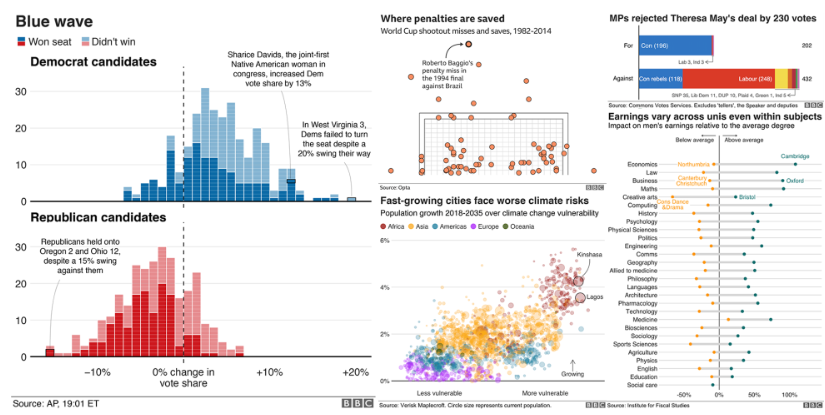
\includegraphics{img/01-bbc.png}
\caption{\label{fig:unnamed-chunk-1}BBC graphs created in R.}
\end{figure}

But why should we learn R and not a different programming language? In contrast to other programming languages (Python, JavaScript, C), R was developed by statisticians. Consequently, R contains an extensive vocabulary to enable us to carry out sophisticated and precise statistical analysis. I have used R and Python to conduct statistical analysis, and anytime I wanted to use a less frequently used statistical test, there was significantly more support and information on how to conduct that analysis in R than in Python. For such reasons, R is typically used among statisticians, social scientists, data miners, and bioinformaticians - and will be used in this course\footnote{There are always tradeoffs in selecting a language. Many programming concepts are easier to grasp in Python than in R. Similarly, there is a lot of resources available for conducting machine-learning analysis in Python.

  But if you are goal is conduct data cleaning, analysis, visualization, and reporting, then R is a excellent choice. The good thing is that once you achieve a certain level of competency in one programming language, you will find it significantly easier to pick up a following one.}.

\hypertarget{create-a-posit-cloud-account.}{%
\section{Create a Posit Cloud Account.}\label{create-a-posit-cloud-account.}}

In the next section, I am going to show you how to download R and RStudio on your desktop. But before we do that, I want you to set up a free account on Posit Cloud (formerly known as RStudio Cloud).

Posit Cloud enables you to use R and RStudio online for free, no need to install anything. There are limitations to this service (you only get so many hours on it with the free account), and I much rather you use your own computers in class. But it will be a handy back-up option in case any technical issues pop up. During class, I might not be able to solve that issue quickly and efficiently, so if it does occur, then you can sign in to Posit Cloud and keep following along with the session.

To create a Posit Cloud account, please follow the following instructions:

\begin{enumerate}
\def\labelenumi{\arabic{enumi}.}
\item
  \href{https://login.posit.cloud/register?redirect=\%2Foauth\%2Fauthorize\%3Fredirect_uri\%3Dhttps\%253A\%252F\%252Fposit.cloud\%252Flogin\%26client_id\%3Dposit-cloud\%26response_type\%3Dcode\%26show_auth\%3D0}{Go to their sign up page website} and enter your details to create an account or Sign up with Google.

  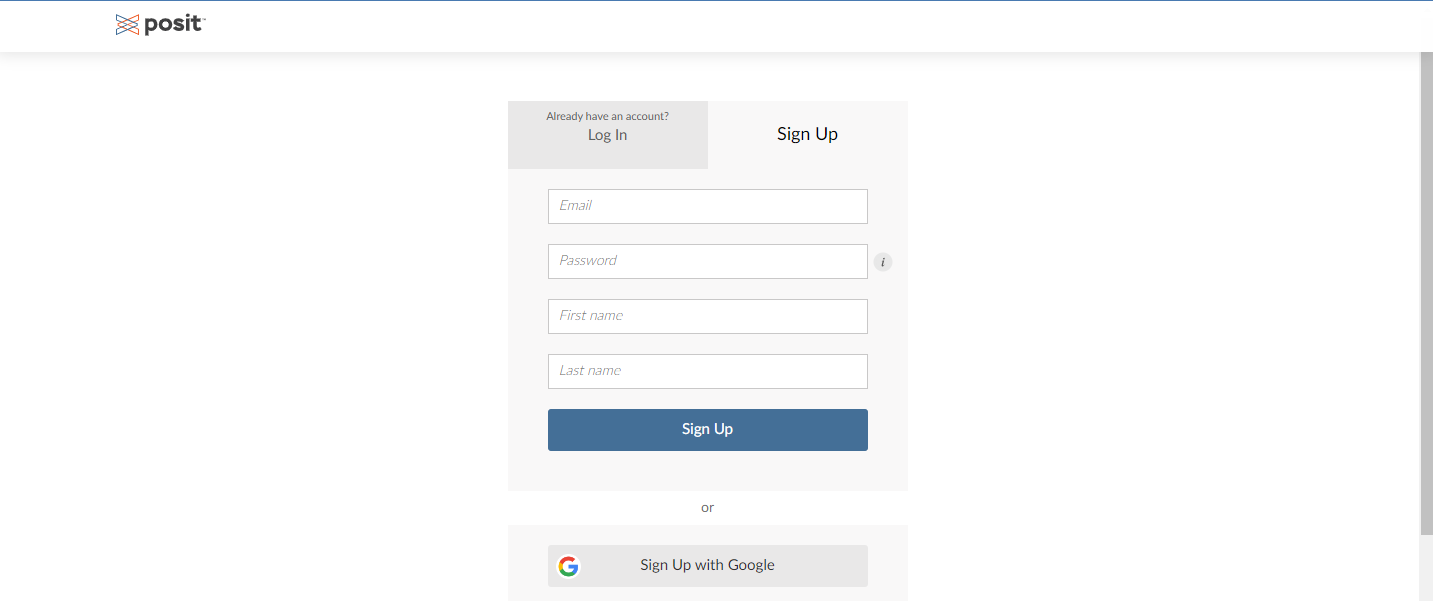
\includegraphics{img/01-posit-sign-up.png}
\item
  Once you have created an account and are in Posit Cloud, click ``New Project'' From the drop-down menu click ``New RStudio Project''. This should take a few seconds to set up (or ``deploy'')
\end{enumerate}

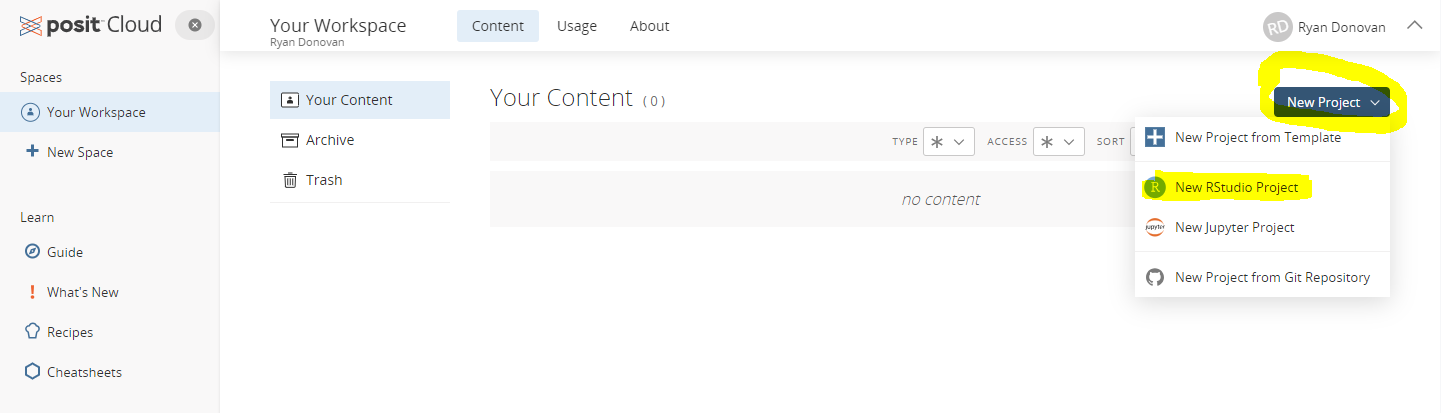
\includegraphics{img/01-posit-newproject.png}

\begin{enumerate}
\def\labelenumi{\arabic{enumi}.}
\tightlist
\item
  Once it is deployed, name your project at the top as \textbf{\emph{rintro}}
\end{enumerate}

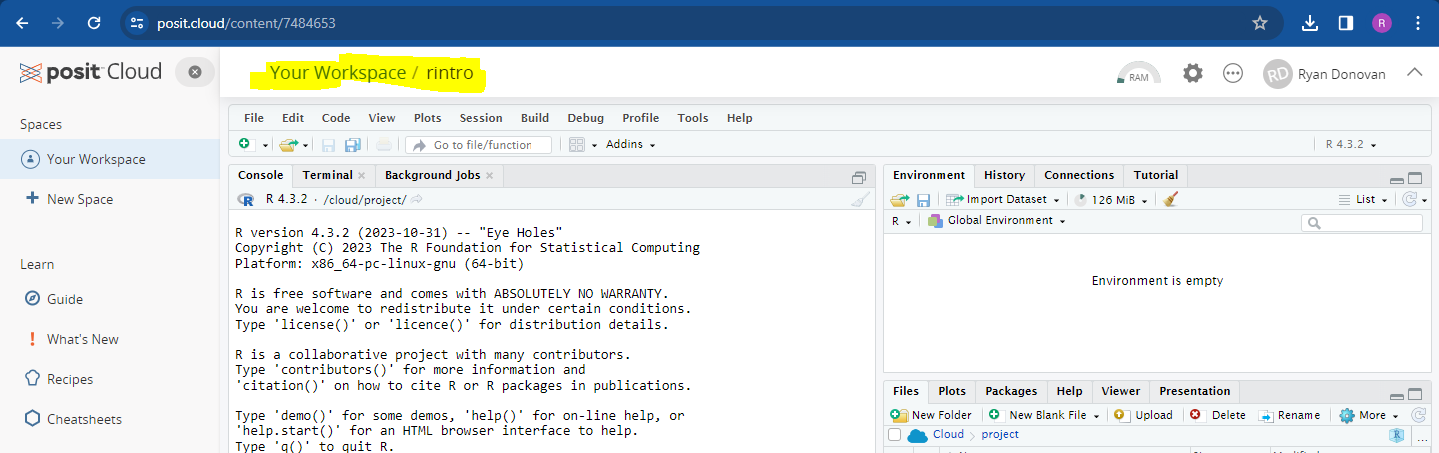
\includegraphics{img/01-posit-rintro.png}

Don't worry about what anything on the screen means for now. We'll come back to that once we download RStudio on your computer. For now, you can sign out of Posit Cloud.

\hypertarget{downloading-r-on-to-your-computer}{%
\section{Downloading R on to your Computer}\label{downloading-r-on-to-your-computer}}

Please follow the following instructions to download R on either Windows or Mac.

\hypertarget{downloading-r-on-windows}{%
\subsection{Downloading R on Windows}\label{downloading-r-on-windows}}

\begin{enumerate}
\def\labelenumi{\arabic{enumi}.}
\tightlist
\item
  Go to the website: \url{https://cran.r-project.org/}
\item
  Under the heading \emph{Download and Install R,} click \emph{Download R for Windows}
\end{enumerate}

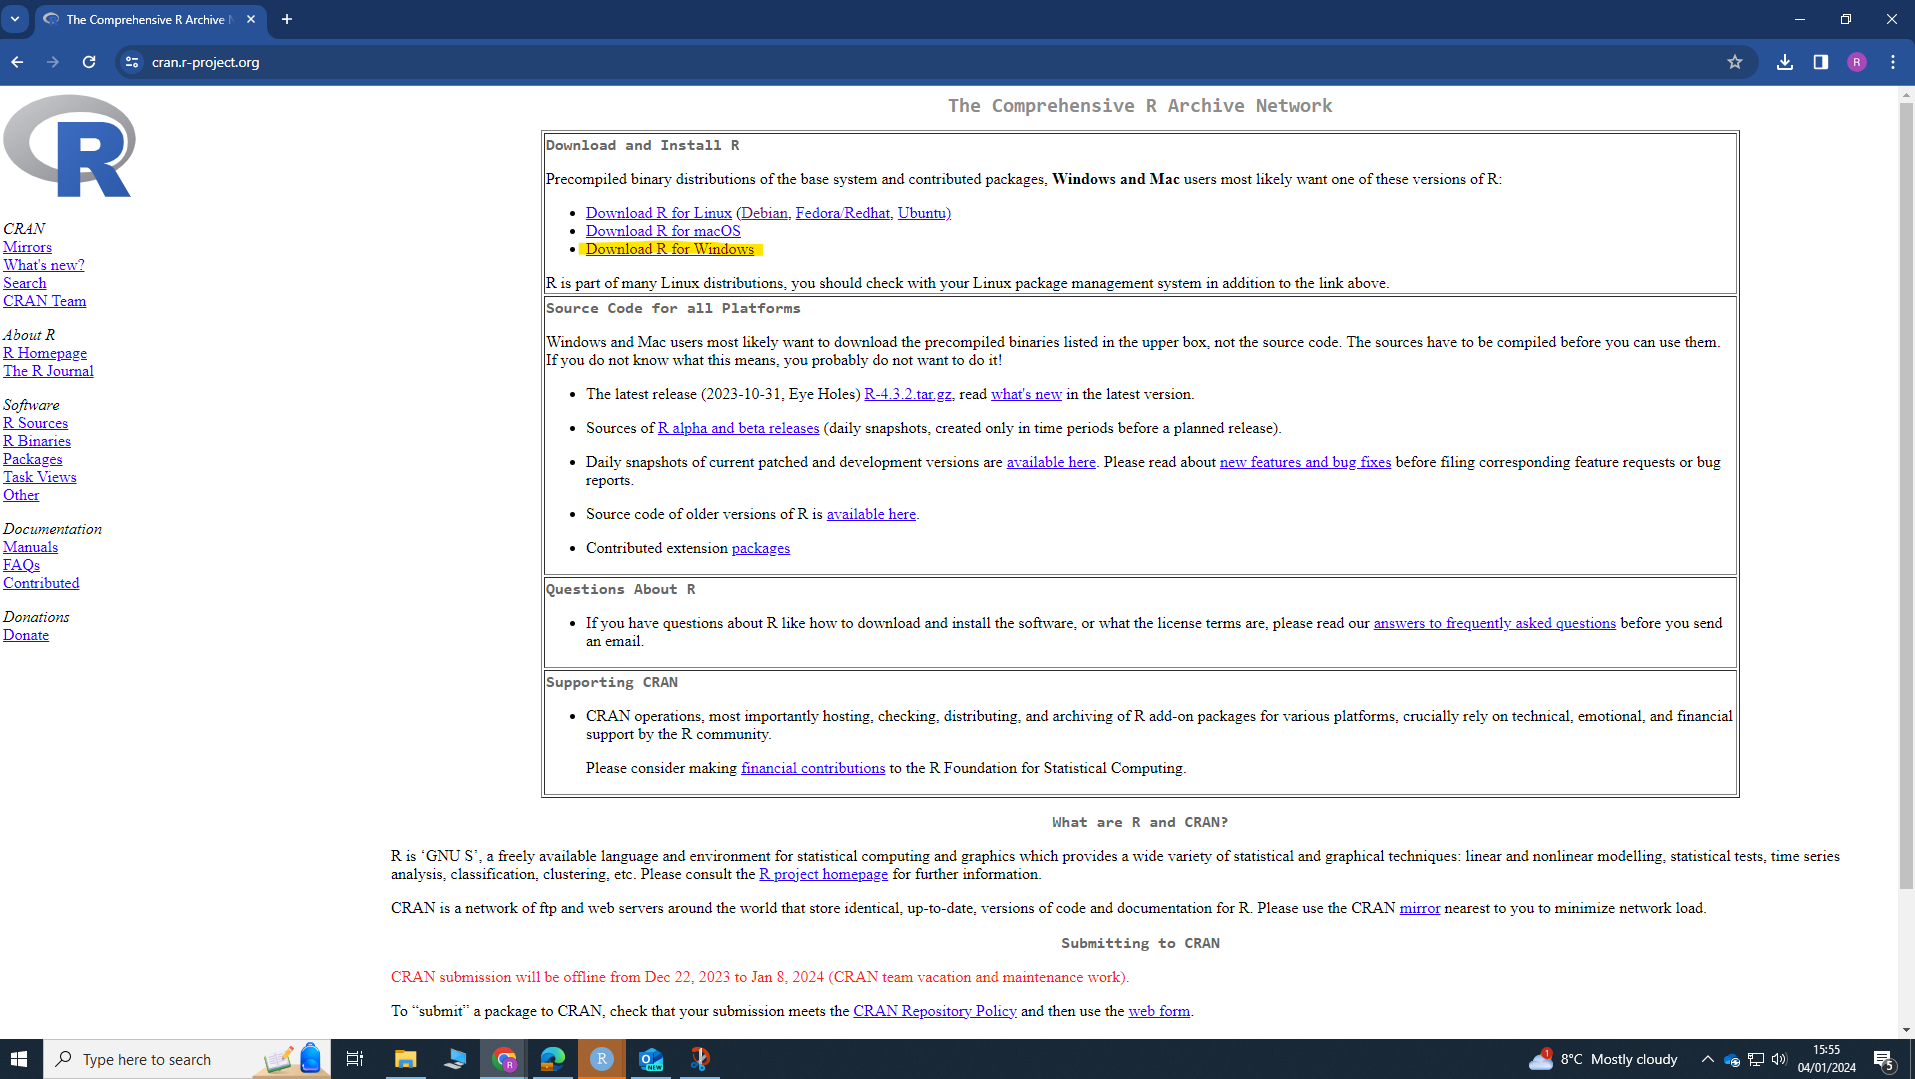
\includegraphics{img/01-cran.png}

\begin{enumerate}
\def\labelenumi{\arabic{enumi}.}
\setcounter{enumi}{2}
\tightlist
\item
  Click the hyperlink \textbf{\emph{base}} or \textbf{\emph{install R for the first Time}}
\end{enumerate}

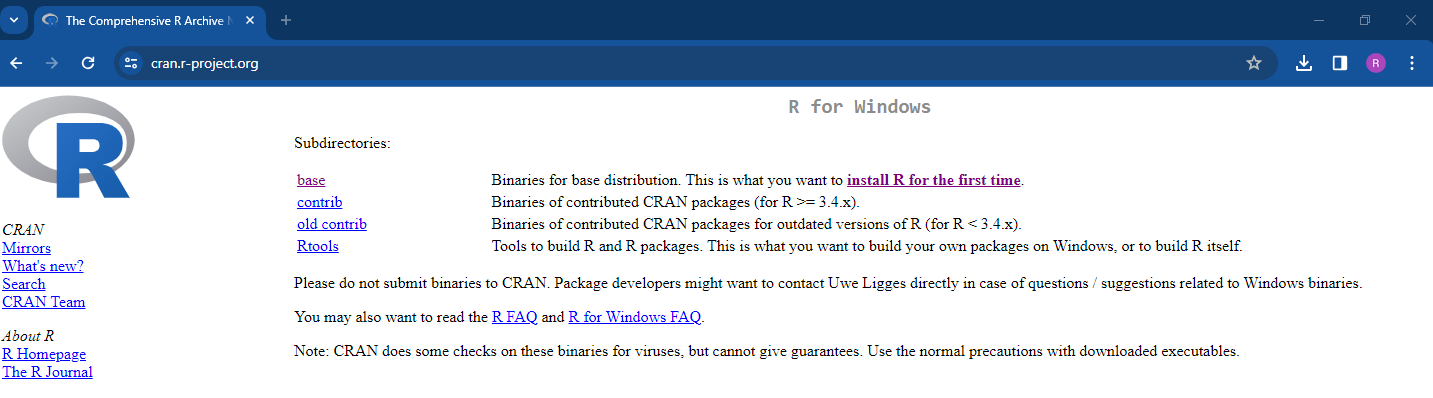
\includegraphics{img/01-base.png}

\begin{enumerate}
\def\labelenumi{\arabic{enumi}.}
\setcounter{enumi}{3}
\tightlist
\item
  Click Download R-4.3.2 for Windows (depending on the date you accessed this, the version of R might have been been updated. That's okay, you can download newer versions). Let the file download.
\end{enumerate}

\begin{figure}
\centering
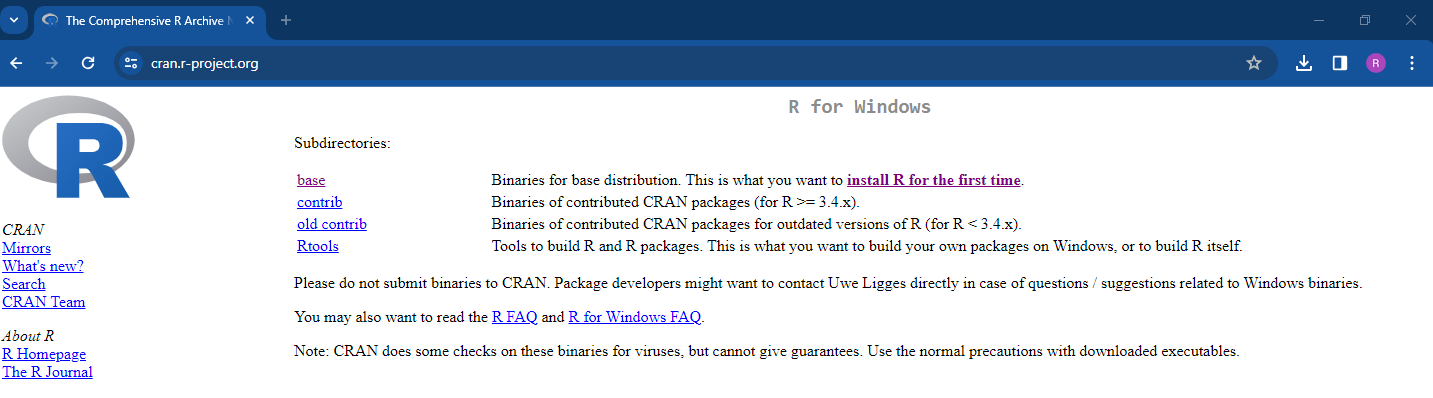
\includegraphics{img/01-base.png}
\caption{\label{fig:unnamed-chunk-7}The R programming language is occasionally updated, so the specific version of R that you see might be different than mine. But that's okay!}
\end{figure}

\begin{enumerate}
\def\labelenumi{\arabic{enumi}.}
\setcounter{enumi}{4}
\tightlist
\item
  Once the file has been downloaded, open it, and click ``Yes'' if you are asked to allow this app to make changes to your device. Then choose English as your setup language. The file name should be something like ``R-4.3.2.-win''. The numbers will differ depending on the specific version that was downloaded.
\item
  Agree to the terms and conditions and select a place to install R. It is perfectly fine to go with the default option.
\end{enumerate}

\hypertarget{downloading-r-on-mac}{%
\subsection{Downloading R on Mac}\label{downloading-r-on-mac}}

The instructions are largely the same for Mac.

\begin{enumerate}
\def\labelenumi{\arabic{enumi}.}
\item
  Go to the website: \url{https://cran.r-project.org/}
\item
  Click Download R for (Mac) OS X.
\end{enumerate}

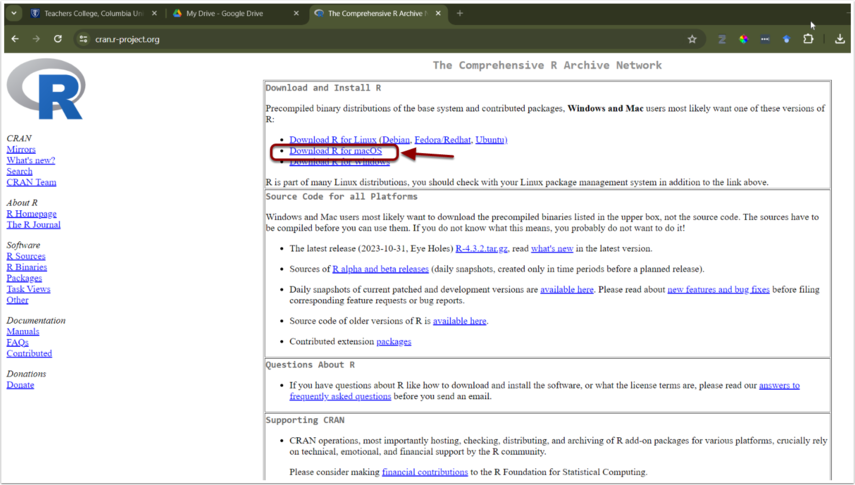
\includegraphics{img/01-rstudiodownload-mac.png}

\begin{enumerate}
\def\labelenumi{\arabic{enumi}.}
\tightlist
\item
  Check the Latest release: section for the appropriate version and follow the directions for download. If you are unsure about this, please ask me.
\end{enumerate}

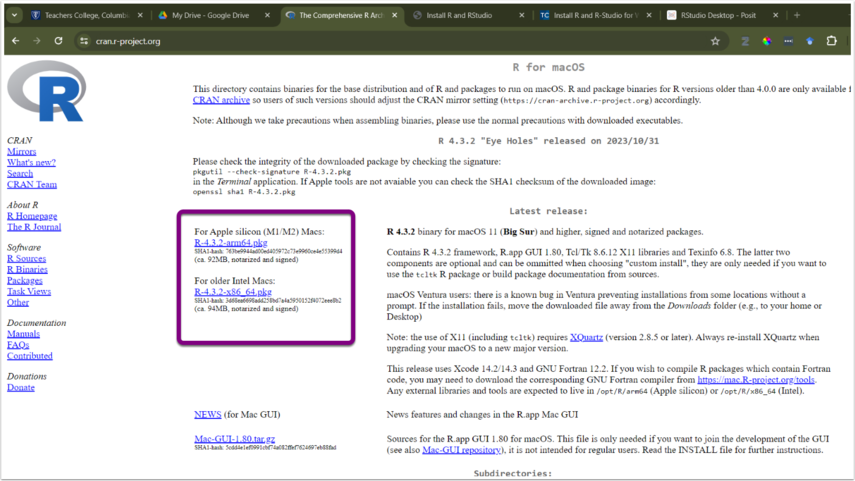
\includegraphics{img/01-rversion-mac.png}

\begin{enumerate}
\def\labelenumi{\arabic{enumi}.}
\tightlist
\item
  Once the file download is complete, click to open the installer. Click Continue and proceed through the installer, I recommend going with all default options.
\end{enumerate}

\begin{figure}
\centering
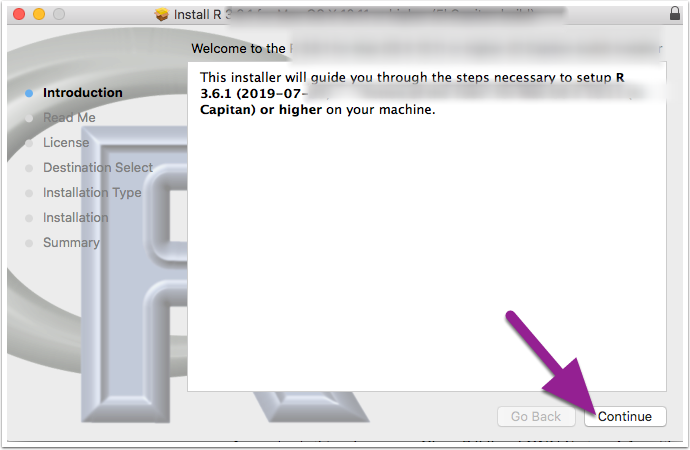
\includegraphics{img/01-mac_installer.png}
\caption{\label{fig:unnamed-chunk-10}Depending on your version of Mac OS, this might look slightly different. But you should still be able to install it.}
\end{figure}

\begin{enumerate}
\def\labelenumi{\arabic{enumi}.}
\tightlist
\item
  Once the R installer has finished, click Close.
\end{enumerate}

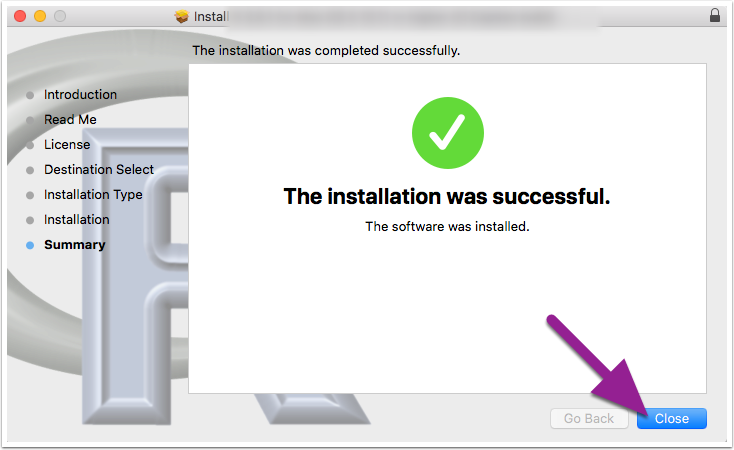
\includegraphics{img/01-install_finish_mac.png}

\hypertarget{install-and-open-r-studio}{%
\section{Install and Open R Studio}\label{install-and-open-r-studio}}

Once R is installed, we will install RStudio.

RStudio is a user-friendly front-end program for R, enhancing your R coding experience without sacrificing any capabilities. RStudio allows us to write and save R code, create plots, manage files, and perform other useful tasks. Think of RStudio as similar to Microsoft Word compared to a basic text editor; while you can write a paper in a text editor, it's much quicker and efficient in Word.

\begin{enumerate}
\def\labelenumi{\arabic{enumi}.}
\tightlist
\item
  \textbf{NB:} Make sure that R is installed \textbf{\emph{before}} trying to install R Studio.
\item
  Go to the RStudio website: \url{https://posit.co/download/rstudio-desktop/}
\item
  The website should automatically detect your operating system. Click the \textbf{\emph{Download RStudio Desktop}} button.
\end{enumerate}

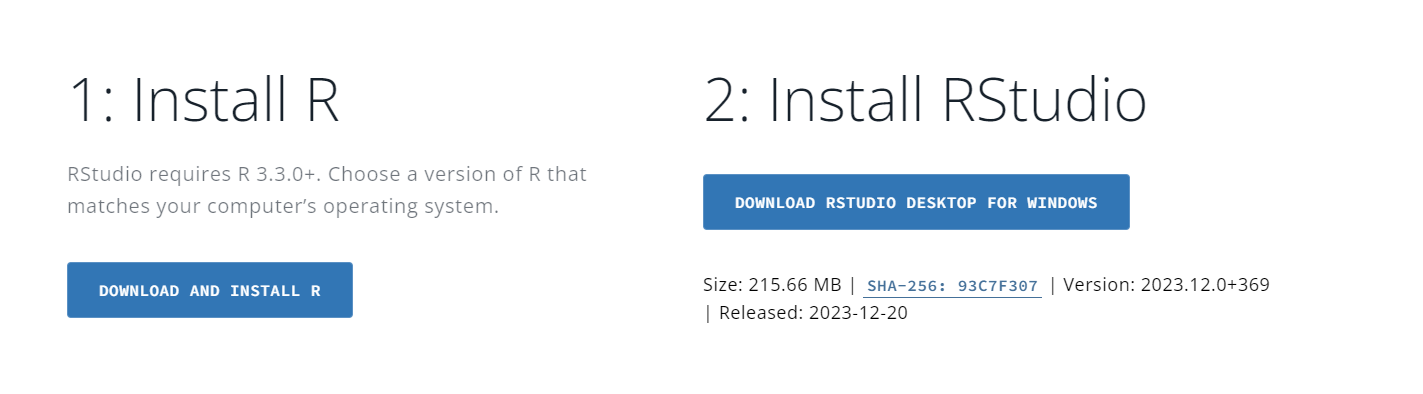
\includegraphics{img/01-rstudiodownload.png}

Once the file is downloaded, open it and allow it to make changes to your device. Then follow the instructions to download the program. I recommend using all the default options during installation.

After downloading both R and RStudio, open RStudio on your computer. You do not have to open R separately, as RStudio will work with R if everything is set up correctly.

When you first open RStudio, you will see three panes or ``windows'' in RStudio: ``Console'' (left), ``Environment'' (top right), and ``Files'' (bottom right).

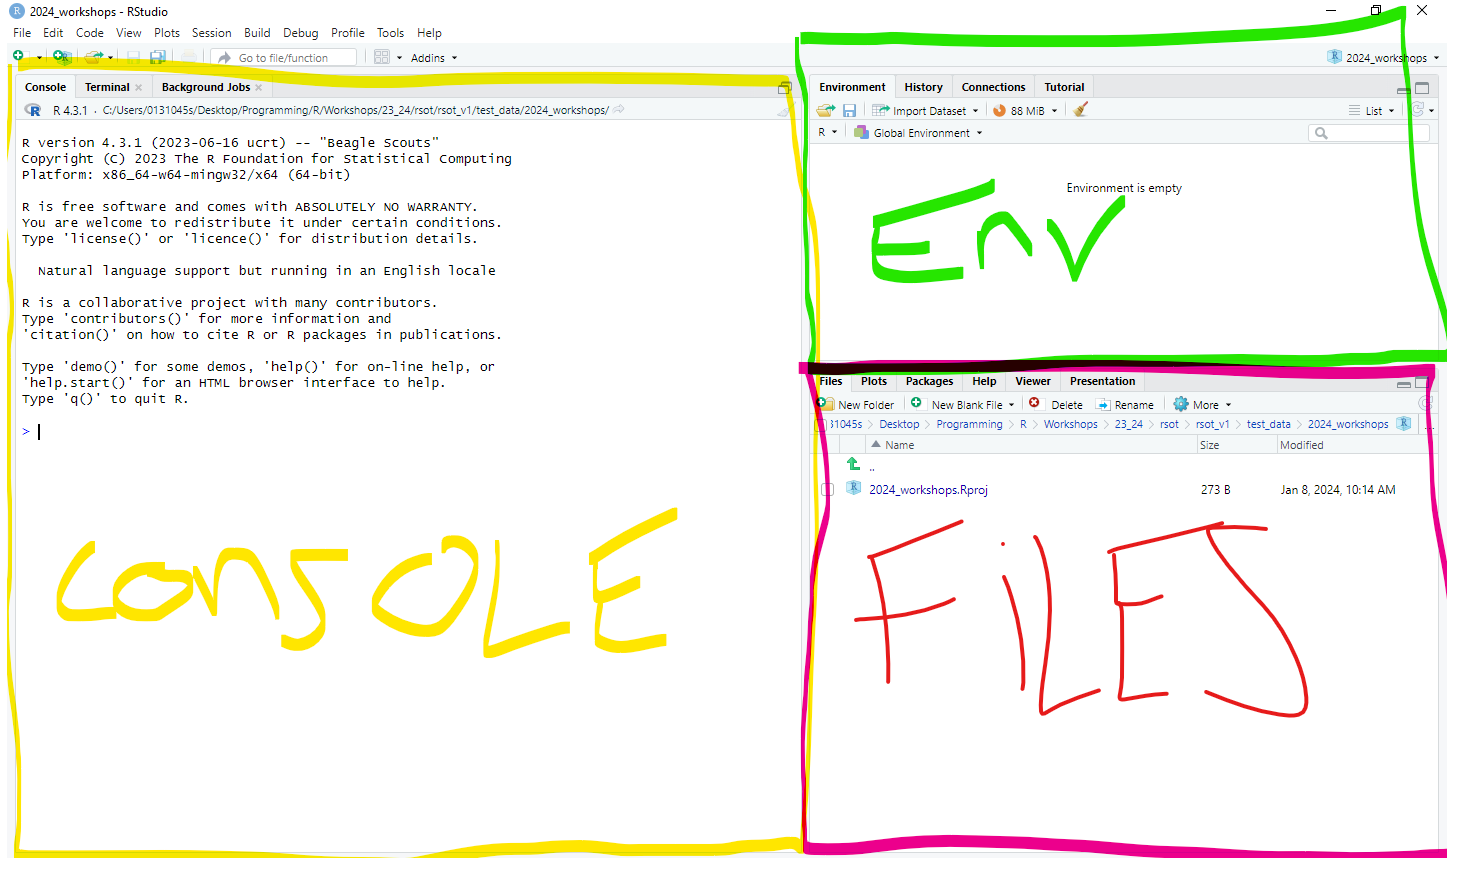
\includegraphics{img/rstudio_first.png}

\hypertarget{creating-an-r-project}{%
\section{Creating an R Project}\label{creating-an-r-project}}

Our first step in RStudio is to create an \emph{R Project}. R Projects are environments that group together input files (e.g., data sets), analyses on those files (e.g., code), and any outputs (e.g., results or plots). Creating an R Project will set up a new directory (folder) on your computer. Whenever you open that project, you are telling R to work within that specific directory.

\textbf{\emph{Activity}}

Let's create an R Project that we will use during these workshops.

\begin{enumerate}
\def\labelenumi{\arabic{enumi}.}
\item
  Click ``File'' in the top left hand corner of RStudio-\textgreater{} then click new ``New Project''
\item
  The ``New Project Wizard'' screen will pop up. Click ``New Directory'' -\textgreater{} ``New Project''
\item
  In the ``Create New Project'' screen, there are four options we are going to change.
\end{enumerate}

\textbf{Option 1}: The ``Directory name'' options sets the name of the project and associated folder.

\begin{itemize}
\item
  You can set this to whatever you want. \textbf{\emph{Just don't set it to ``R'',}} as this can create problems down the line.
\item
  I \textbf{\emph{recommend}} that you set the same directory name as me - \textbf{\emph{rintro}}
\end{itemize}

\textbf{Option 2}: The ``Create project as sub-directory of'' option selects a place to store this project on your computer.

\begin{itemize}
\item
  You can save it anywhere you like (e.g., your Desktop). Just ensure it's in a place you can easily find and where it won't be moved (e.g., if you save folders to your desktop but tend to relocate them later, avoid saving it on your desktop).
\item
  My recommendation is to create a folder called ``R\_Programming'' on your desktop and save your project inside this folder.
\item
  Regardless of where you save your project, copy the location and keep it in a place you can check later (e.g., in a text file).
\end{itemize}

\textbf{Option 3}: The ``Use renv with this project'' option enables you to create a virtual environment for this project that will be separate to other R projects. Don't worry for now about what that means, it will be explained later on.

\begin{itemize}
\tightlist
\item
  Tick this option.
\end{itemize}

\textbf{Option 4:} The ``Open in new session'' just opens a new window on RStudio for this project.

\begin{itemize}
\tightlist
\item
  Tick this option.
\end{itemize}

\textbf{Note on Github Repository}: This will probably not appear on your RStudio project, but that's okay, you don't need it for this course.

You can see my example below. Once you're happy with your input for each option, click ``Create Project'' This will open up the project \textbf{\emph{rintro}}.

\begin{figure}
\centering
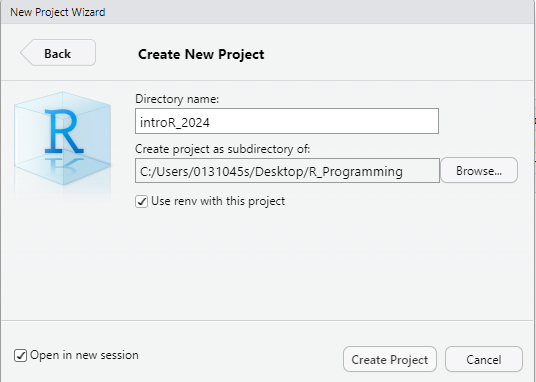
\includegraphics{img/01-newproject.png}
\caption{\label{fig:unnamed-chunk-14}New Project Set Up}
\end{figure}

\hypertarget{navigating-rstudio}{%
\subsection{Navigating RStudio}\label{navigating-rstudio}}

In our new project, \textbf{\emph{rintro}}, we are going to open the ``Source'' pane, which we will often use for writing code, and viewing datasets.

There are a variety of ways to open the Source pane.

\textbf{Button approach}: Click the ``File'' tab in the top-left hand corner (not the File pane) -\textgreater{} Click ``New File'' -\textgreater{} ``R Script''

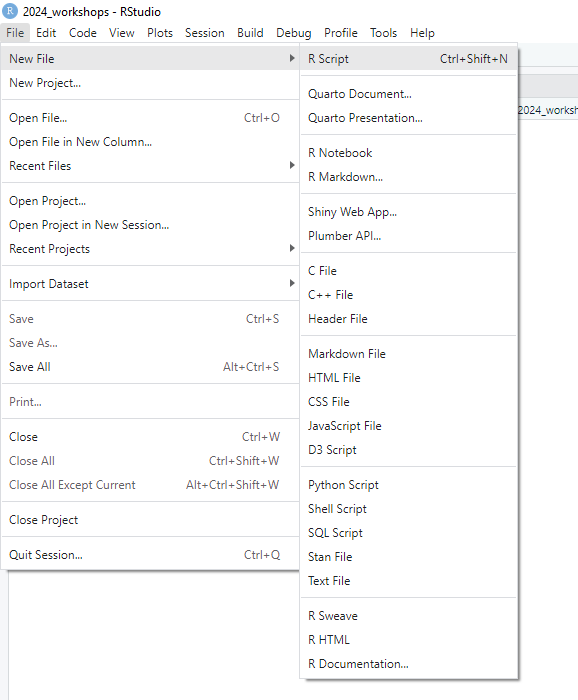
\includegraphics{img/rstudio_create_file.png}

\textbf{\emph{Button Shortcut}}: directly underneath the \emph{File} tab, there is an icon of a white sheet with a green and white addition symbol. You can click that too.

\textbf{Keyboard Shortcut:} You can press ``Ctrl'' + ``Shift'' and ``N'' on Windows. Or ``Cmd'' + ``Shift'' + ``N'' on Mac.

Now you should see your four panes: Source, Console, Environment, and Files.

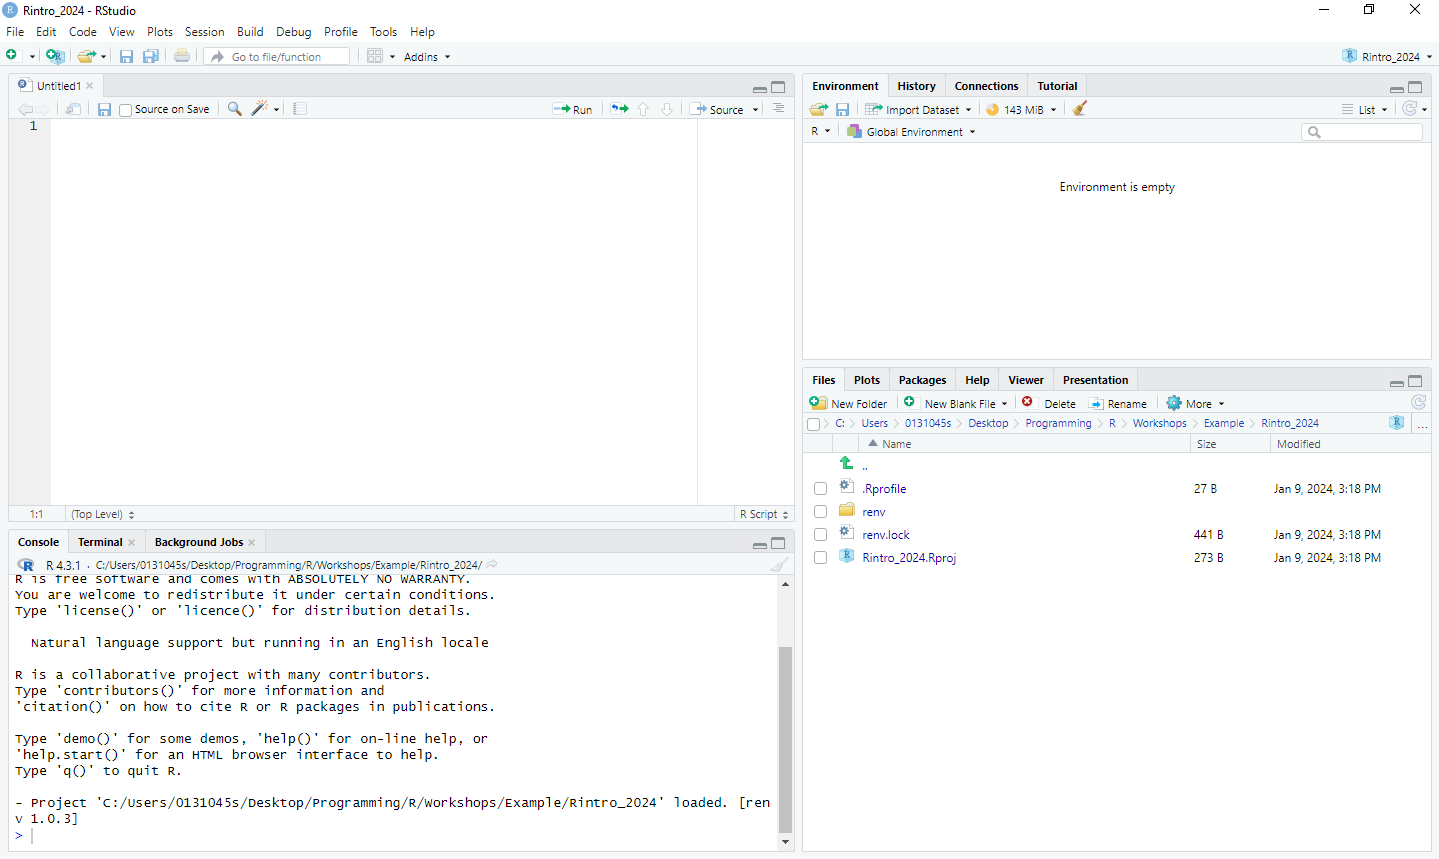
\includegraphics{img/01-four-panes.png}

\hypertarget{the-rstudio-workspace}{%
\subsubsection{The RStudio Workspace}\label{the-rstudio-workspace}}

With each pane opened, let's briefly describe their purposes.

\begin{itemize}
\item
  The \textbf{\emph{Source Pane}} is where you will write R scripts. R scripts enable you to write, save, and run R code in a structured format. For instance, you might have an R script titled ``Descriptive,'' containing the code for computing descriptive statistics on your data set. Similarly, you might have another R script titled ``Regression'' for performing regression analyses in R.
\item
  The \textbf{\emph{Console Pane}} is where you can write R code or enter commands into R. The console is also where you can find various outputs from your R scripts. For example, if you create a script for running a t-test in R, the results will appear in the Console Pane. Any error or warning messages related to your code will also be highlighted in the console. In short, the console is where R actually runs.
\item
  The \textbf{\emph{Environment Pane}} contains information about data sets and variables imported or created in R within a specific R project. The ``History'' tab shows a history of the R code executed during the project. This pane is helpful for getting an overview of a project, especially if you return to it after a long time or are reviewing someone else's code.
\item
  The \textbf{\emph{Files Pane}} includes your R project files (Files tab), the output of any plots you create (Plots tab), the status of downloaded packages (Packages tab), and information about R functions and packages (Help).
\end{itemize}

All four panes will be used extensively during these workshops.

\hypertarget{checking-our-working-directory}{%
\subsection{Checking our Working Directory}\label{checking-our-working-directory}}

Every time you open a project or file in RStudio, it's good practice to check the working directory. The working directory is the environment on your computer where R is currently operating.

Ideally, you want the working directory to match the location of your R project. This ensures that any files you import into RStudio or any files you export (datasets, results, graphs) can be easily found in your R project folder. Checking the working directory can help prevent many common R problems. To check the working directory, type the following into the console pane:

\begin{Shaded}
\begin{Highlighting}[]
\FunctionTok{getwd}\NormalTok{()}
\end{Highlighting}
\end{Shaded}

\begin{verbatim}
## [1] "C:/Users/0131045s/Desktop/Programming/R/Workshops/rintro"
\end{verbatim}

This will display the current working directory where R is operating. Your working directory will likely differ from mine, which is normal. Just confirm that it matches the location you specified when creating your project (\textbf{Option 2}).

\hypertarget{set_wd}{%
\subsection{Setting up a new Working Directory}\label{set_wd}}

We are going to slightly change our working directory. In our R Project, we are going to create a folder for week1 of the workshop. Anything that we create in R will then be saved into this week1 folder.

\begin{itemize}
\tightlist
\item
  Click ``Session'' on your RStudio toolbar -\textgreater{} Set Working Directory -\textgreater{} Choose Directory
\end{itemize}

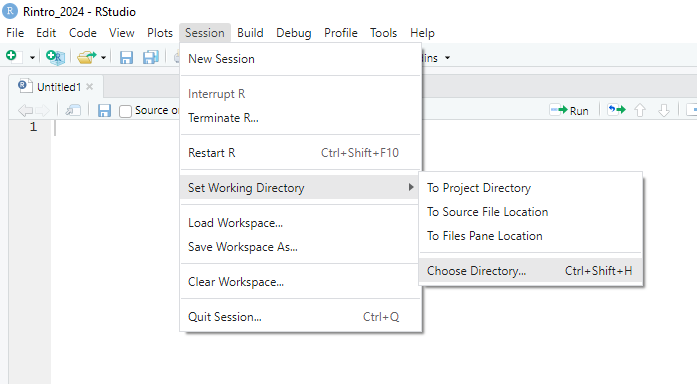
\includegraphics{img/01-wd.png}

\begin{itemize}
\item
  By default you should be in your R Project (e.g., \textbf{\emph{rintro}}).
\item
  Within this R Project, create a new folder and call it ``week1''
\item
  Click ``week1'' and then click Open
\end{itemize}

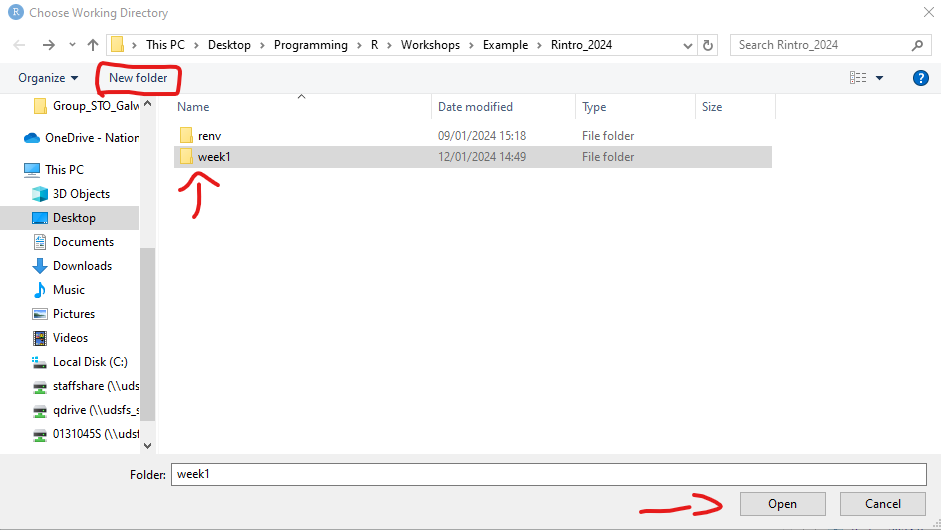
\includegraphics{img/01-new_wd.png}

You should see something like the following in your console

\begin{verbatim}
> setwd("C:/Users/0131045s/Desktop/Programming/R/Workshops/rintro/week1")
\end{verbatim}

Check whether this is actually the location you want to store your files for this course. If it is, we are good to go. If not, then let me know.

\hypertarget{writing-our-first-r-code}{%
\section{Writing our first R Code}\label{writing-our-first-r-code}}

Let's write our first line of R code in the console. The R console uses the prompt symbol \textgreater{} to indicate that it is ready for a new line of code.

Type in each of the following instructions (after the \textgreater{} operator) and press enter. Feel free to change the second line of code to add your own name.

\begin{Shaded}
\begin{Highlighting}[]
\FunctionTok{print}\NormalTok{(}\StringTok{"Hello World"}\NormalTok{)}
\end{Highlighting}
\end{Shaded}

\begin{verbatim}
## [1] "Hello World"
\end{verbatim}

\begin{Shaded}
\begin{Highlighting}[]
\FunctionTok{print}\NormalTok{(}\StringTok{"My name is Ryan and I am learning to code in R"}\NormalTok{)}
\end{Highlighting}
\end{Shaded}

\begin{verbatim}
## [1] "My name is Ryan and I am learning to code in R"
\end{verbatim}

Congratulations, you've written your first piece of code!

Let's describe what is going on here. We used a function called print() to print the words ``Hello World'' and ``My name is Ryan, and I am learning to code in R'' in the console. Functions are equivalent to verbs in the English language - they describe doing things. In this case, R sees the function print - then it looks inside the bracket to see what we want to print, and then it goes ahead and prints it. Pretty straightforward.

Functions are a very important programming concept, and there is a lot more going on under the hood than I have described so far - so we will be returning to functions repeatedly and filling you in with more information. But in essence, functions are verbs that enable us to tell our computer to carry out specific actions on objects.

\hypertarget{console-vs-source-script}{%
\section{Console vs Source Script}\label{console-vs-source-script}}

You might have noticed that I asked you to write code in the console rather than in the source pane. It's worth discussing here what the differences are between the console and the script when it comes to writing code.

The console is like the immediate chat with R. It's where you can type and execute single lines of code instantly. Imagine it as a friendly conversation where you ask R to perform a task, and it responds immediately. The console is great for experimenting and getting instant feedback. It's your interactive playground, perfect for spontaneous interactions with R.

The console is also really useful for performing quick calculations, testing functions or pieces of code, and for running code that should run once and only once.

However, the console is cumbersome to use if we want to write code that is several lines long and/or when we want to structure or save our code. This is where R scripts come in.

R scripts are text files where we can write R code in a structured manner. Scripts enable us to structure our code (e.g., with headings and instructions), write several pieces of code, and save and rerun code easily. If you think of your console as a draft, then your script is for the code that you want to keep.

From now on, whenever we write code, we are going to be using R scripts by default. For the times we will write code in the console, I will let you know beforehand.

\hypertarget{lets-write-some-statistical-code}{%
\section{Let's write some statistical code}\label{lets-write-some-statistical-code}}

Okay, we have talked a lot about R and RStudio. To finish off this session, let's write code that will take a data set, calculate some descriptive statistics, run an inferential test, generate a graph, and save our results. Don't worry if you don't understand all of the code provided below. Just follow along and type it yourself in the R script we opened up earlier (if it's not open, click ``File'' -\textgreater{} ``New File'' -\textgreater{} ``RScript''). Once you have created this script, save it as ``01-paired-t-tests''.

When you download R, you will have automatic access to several functions (e.g., print) and data sets. One of these data sets is called sleep, which we are going to use right now. To learn more about the sleep data set, type \textbf{\texttt{?sleep}} into the console. You will find more information on the data sets in the Files pane, under the Help tab.

First, let's have a look at the sleep data set by writing the following code in the R script. To run scripts in R, select the code you have written and click the Run button with the green arrow in the top right corner of the script.

\begin{Shaded}
\begin{Highlighting}[]
\FunctionTok{print}\NormalTok{(sleep) }
\end{Highlighting}
\end{Shaded}

\begin{verbatim}
##    extra group ID
## 1    0.7     1  1
## 2   -1.6     1  2
## 3   -0.2     1  3
## 4   -1.2     1  4
## 5   -0.1     1  5
## 6    3.4     1  6
## 7    3.7     1  7
## 8    0.8     1  8
## 9    0.0     1  9
## 10   2.0     1 10
## 11   1.9     2  1
## 12   0.8     2  2
## 13   1.1     2  3
## 14   0.1     2  4
## 15  -0.1     2  5
## 16   4.4     2  6
## 17   5.5     2  7
## 18   1.6     2  8
## 19   4.6     2  9
## 20   3.4     2 10
\end{verbatim}

The \textbf{\texttt{print()}} function here prints out the sleep data set in the console. There are also other ways to view a data set, such as using the functions \textbf{\texttt{head()}}, \textbf{\texttt{tail()}}, \textbf{\texttt{View()}}, and \textbf{\texttt{str()}}. Type these in the console (make sure to put \textbf{\texttt{sleep}} inside the brackets) and see what results you get.

The result of \textbf{\texttt{print(sleep)}} shows us there are 20 observations in the dataset (rows), with three different variables (columns): extra (hours of extra sleep each participant had), group (which treatment they were given), and ID (their participant ID).

Now let's calculate some descriptive statistics. One way we can do this is by using the \textbf{\texttt{summary()}} function. This function takes in an object (e.g., like a data set) and summarizes the data. Write the following in your R script and press run.

\begin{Shaded}
\begin{Highlighting}[]
\FunctionTok{summary}\NormalTok{(sleep) }
\end{Highlighting}
\end{Shaded}

\begin{verbatim}
##      extra        group        ID   
##  Min.   :-1.600   1:10   1      :2  
##  1st Qu.:-0.025   2:10   2      :2  
##  Median : 0.950          3      :2  
##  Mean   : 1.540          4      :2  
##  3rd Qu.: 3.400          5      :2  
##  Max.   : 5.500          6      :2  
##                          (Other):8
\end{verbatim}

Running \textbf{\texttt{summary(sleep)}} shows us descriptive statistics for each of our variables. We can see that the mean change in hours of sleep was +1.5, and that there were 10 participants in both the control and experimental condition.

But it's not exactly what we need. Firstly, we don't need summary descriptives on the participant ID. Secondly, it only tells us the mean of the entire sample, whereas we want the mean score for each treatment group. To get this information, we can use the \textbf{\texttt{aggregate()}} function, which enables us to split our data into subsets and then compute summary statistics per group. Remember to press run after you've written your code.

\begin{Shaded}
\begin{Highlighting}[]
\CommentTok{\#The code inside the aggregate bracket tells our computer to: }
\CommentTok{\# data = sleep {-}\textgreater{} Go to the sleep data set}

\CommentTok{\#extra \textasciitilde{} group {-}\textgreater{} Take the variable "extra" and split it into subsets based on the variable "group"}

\CommentTok{\# FUN = mean {-}\textgreater{} Apply the mean() function (FUN) on each subset }

\FunctionTok{aggregate}\NormalTok{(}\AttributeTok{data =}\NormalTok{ sleep, extra }\SpecialCharTok{\textasciitilde{}}\NormalTok{ group, }\AttributeTok{FUN =}\NormalTok{ mean)}
\end{Highlighting}
\end{Shaded}

\begin{verbatim}
##   group extra
## 1     1  0.75
## 2     2  2.33
\end{verbatim}

That's more like it. Now we can see that there does seem to be a difference between treatment1 and treatment2. Participants slept an extra 2.33 hours on average when taking treatment 2, whereas they only slept 0.75 hours (e.g., 45 minutes) more on average when taking treatment 1. So, treatment 2 does seem more effective.

Let's run a paired-samples t-test to see if those differences are significant (I have assumed all parametric assumptions are correct).

\begin{Shaded}
\begin{Highlighting}[]
\FunctionTok{t.test}\NormalTok{(sleep}\SpecialCharTok{$}\NormalTok{extra[sleep}\SpecialCharTok{$}\NormalTok{group }\SpecialCharTok{==} \DecValTok{1}\NormalTok{], }\CommentTok{\#this code extracts the group 1 scores}
\NormalTok{       sleep}\SpecialCharTok{$}\NormalTok{extra[sleep}\SpecialCharTok{$}\NormalTok{group }\SpecialCharTok{==} \DecValTok{2}\NormalTok{], }\CommentTok{\# this code extracts group 2 scores}
       \AttributeTok{paired =} \ConstantTok{TRUE}\NormalTok{) }\CommentTok{\#this code tells R to run a paired t{-}test, not between/independent t{-}test}
\end{Highlighting}
\end{Shaded}

\begin{verbatim}
## 
##  Paired t-test
## 
## data:  sleep$extra[sleep$group == 1] and sleep$extra[sleep$group == 2]
## t = -4.0621, df = 9, p-value = 0.002833
## alternative hypothesis: true mean difference is not equal to 0
## 95 percent confidence interval:
##  -2.4598858 -0.7001142
## sample estimates:
## mean difference 
##           -1.58
\end{verbatim}

Boom! We can see there is a statistically significant difference between the two groups. I know the code within the t-test might look a bit complicated, but we will break it down and explain it as we go on in further weeks.

Finally, let's visualize our data with the plot() function.

\begin{Shaded}
\begin{Highlighting}[]
\FunctionTok{plot}\NormalTok{(sleep}\SpecialCharTok{$}\NormalTok{group, sleep}\SpecialCharTok{$}\NormalTok{extra)}
\end{Highlighting}
\end{Shaded}

\begin{figure}
\centering
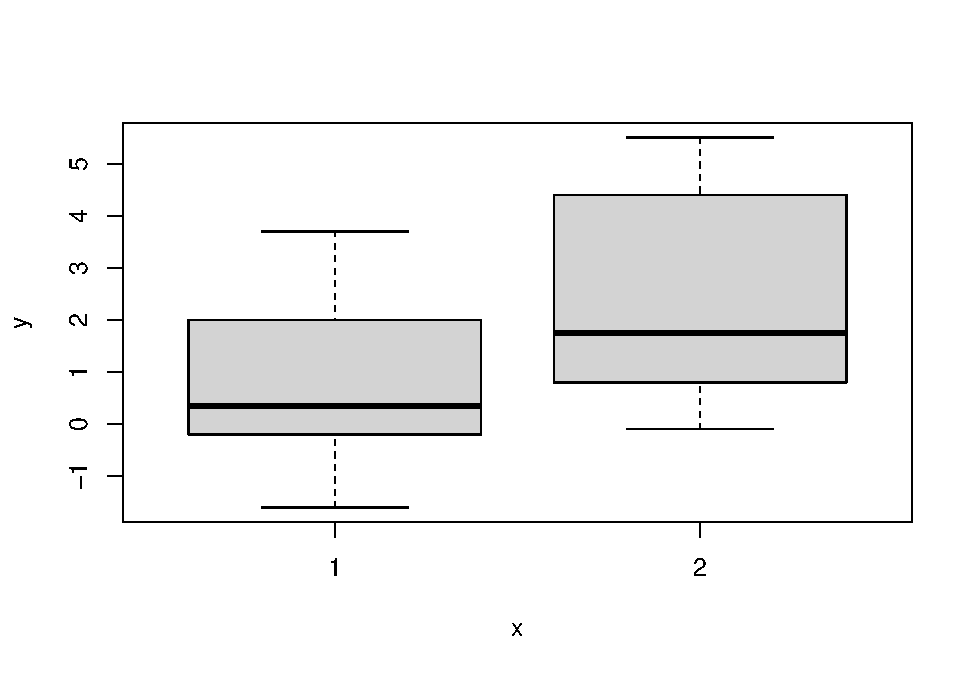
\includegraphics{rintro_demo_files/figure-latex/unnamed-chunk-24-1.pdf}
\caption{\label{fig:unnamed-chunk-24}Generic Boxplot}
\end{figure}

The \texttt{plot()} function is an example of a generic function, which means it adapts to our code. In this case, the plot() function looks at the variables we want to plot and identifies that the box plot is the most appropriate way to plot it.

Now this plot is perfectly adequate for a first viewing, but let's make it a bit more instructive by adding labels to the x and y-axes, and by adding a title to it.

\begin{Shaded}
\begin{Highlighting}[]
\CommentTok{\#xlab = creates a label for the x{-}axis  }

\CommentTok{\#ylab = creates a title for the y{-}axis  }

\CommentTok{\#main = creates a title for the plot  }



\FunctionTok{plot}\NormalTok{(sleep}\SpecialCharTok{$}\NormalTok{group, sleep}\SpecialCharTok{$}\NormalTok{extra, }\AttributeTok{xlab =} \StringTok{"Treatment"}\NormalTok{, }\AttributeTok{ylab =} \StringTok{"Hours of Sleep"}\NormalTok{, }\AttributeTok{main =} \StringTok{"Effect of Treament on Sleep Duration"}\NormalTok{)  }
\end{Highlighting}
\end{Shaded}

\begin{figure}
\centering
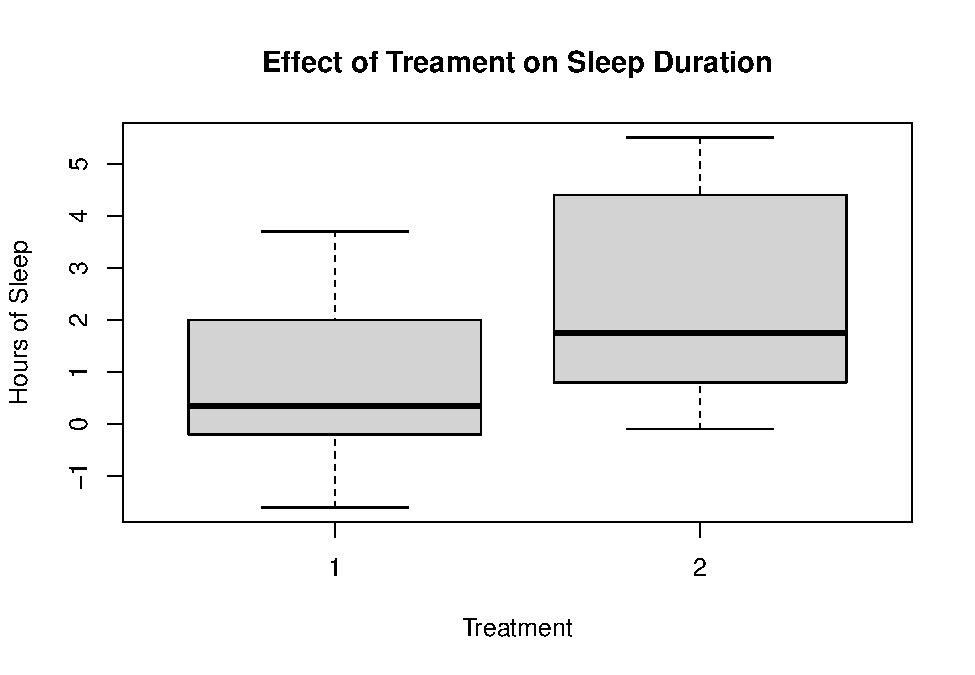
\includegraphics{rintro_demo_files/figure-latex/unnamed-chunk-25-1.pdf}
\caption{\label{fig:unnamed-chunk-25}Generic Boxplot with appropriate labelling}
\end{figure}

Now let's take this plot and save it to a PDF so that we can share our results with others. The standard way of doing this in R is a bit cumbersome. We have to tell R that we are about to create a plot that we want to make into a PDF. Then we have to generate the plot. Then we have to tell R we are done with creating the PDF. We'll learn a MUCH simpler way to do this in future weeks, but this will do for now.

\begin{Shaded}
\begin{Highlighting}[]
\FunctionTok{pdf}\NormalTok{(}\AttributeTok{file =} \StringTok{"myplot.pdf"}\NormalTok{) }\CommentTok{\#Tells R that we will create a pdf file called "my\_plot" in our working directory}

\FunctionTok{plot}\NormalTok{(sleep}\SpecialCharTok{$}\NormalTok{group, sleep}\SpecialCharTok{$}\NormalTok{extra, }\AttributeTok{xlab =} \StringTok{"Treatment"}\NormalTok{, }\AttributeTok{ylab =} \StringTok{"Hours of Sleep"}\NormalTok{, }\AttributeTok{main =} \StringTok{"Effect of Treament on Sleep Duration"}\NormalTok{)  }\CommentTok{\#this will save the plot to our pdf}


\FunctionTok{dev.off}\NormalTok{() }\CommentTok{\#this tells R that we are done with adding stuff to our PDF}
\end{Highlighting}
\end{Shaded}

\begin{verbatim}
## pdf 
##   2
\end{verbatim}

Go to the files pane, and open up the pdf ``myplot.pdf''. It should be in your working directory. Open it up the PDF and have a look at your graph\footnote{This is a fairly generic type of graph offered by base R. During the course we will looking at ways we can create ``sexier'' and more APA friendly type of graphs. But for one line of code, it's not bad!}.

\hypertarget{comments}{%
\subsection{Comments}\label{comments}}

One last concept before we finish. You might have noticed that I wrote several things with a \textbf{\texttt{\#}} before them. These are known as comments. Comments are any piece of text that will be ignored by R (i.e., they will not be executed within the console). They are fundamental to writing clear code.

We create comments using the \textbf{\texttt{\#}} symbol. This symbol tells R to ignore whatever comes directly \textbf{\emph{afterwards}}.

There are various reasons for using comments.

\begin{figure}
\centering
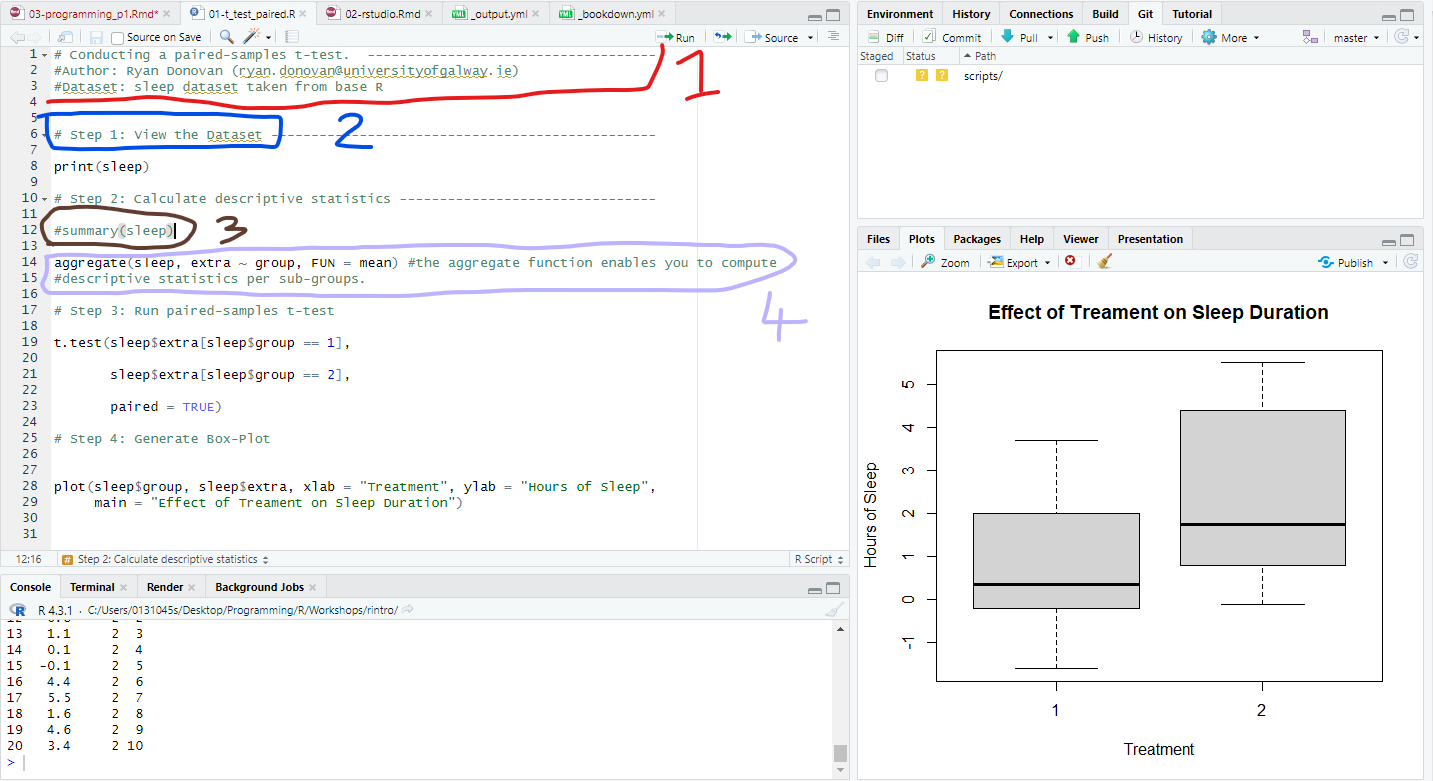
\includegraphics{img/03-comments.png}
\caption{\label{fig:unnamed-chunk-27}Four Examples of Comments Use}
\end{figure}

In the above figure, you'll see four different types of comments.

\begin{enumerate}
\def\labelenumi{\arabic{enumi}.}
\item
  The first type of comment provides a quick introduction to the R script. It can be really useful here to provide clear information on what this script is trying to do (e.g., run a paired samples t-test), what data it is working on (the sleep dataset), and who wrote or developed this script. This makes it significantly easier for anyone who might be reviewing your work or trying to apply your code to their own work to understand what is going on.
\item
  The second type of comment structures the format of the script by providing headings or steps. Again, this just makes it easier to understand what is going on.
\item
  The third type of comment is placed before the summary. This means that the code \textbf{\texttt{summary(sleep)}} will not be executed in R. Why would we do this? If you remember last week, we wanted to compute the mean per each of our two treatment groups, which the summary function does not enable us to do, so it's not part of our main analysis. So why keep it? Well, it still provides us with valuable information (e.g., mean, median, min, max for the entire sample), so rather than delete it, we'll just put a comment in front of it. And if any time we want to check these descriptives, we can just remove the \textbf{\texttt{\#}} and run that line of code.
\item
  The fourth type of comment provides some context or information on what a specific line of code is doing, namely, what the \textbf{\texttt{aggregate()}} function does. Again, this is really useful, particularly if you are using functions that are not well-known.
\end{enumerate}

Comments are extremely useful for orienting yourself to code. My advice would be to comment as much as your code as you. Anyone who has coded will have experienced the following situation - You spend days/weeks writing a piece of code to clean a messy data set and run a specialized type of analysis. Several months go by, and you need to return to your data set (pesky reviewer \#2 wants you to change something). You open up your R script, and you are \textbf{\emph{completely lost}}. You have written no comments, so you have to spend days trying to remember what each piece of code was trying to do.

If you comment a lot, it will save you so much heartache in the future. And it will help you understand various code concepts better if you can explain them while you are using them. So comment, comment, comment!

\hypertarget{summary}{%
\section{Summary}\label{summary}}

There we have it! That completes our first session with R and RStudio. Today was more about getting to grips with the software R and RStudio, but we still got our first pieces of code written. Hopefully, it's given you a tiny glimpse into what R can do.

In the next two sessions, we will learn basic programming concepts and how to import data in R.

\hypertarget{glossary}{%
\section{Glossary}\label{glossary}}

This glossary defines key terms introduced in Chapter 2.

\begin{longtable}[]{@{}
  >{\raggedright\arraybackslash}p{(\columnwidth - 2\tabcolsep) * \real{0.2706}}
  >{\raggedright\arraybackslash}p{(\columnwidth - 2\tabcolsep) * \real{0.7294}}@{}}
\toprule\noalign{}
\begin{minipage}[b]{\linewidth}\raggedright
Term
\end{minipage} & \begin{minipage}[b]{\linewidth}\raggedright
Definition
\end{minipage} \\
\midrule\noalign{}
\endhead
\bottomrule\noalign{}
\endlastfoot
Comment & Text in an R script that is ignored by R. Comments are preceded by the \texttt{\#} symbol and are used to add explanations, headings, or disable code temporarily. \\
Console & The interactive interface in RStudio where you can type and execute R commands and see their immediate output. \\
Environment Pane & The pane in RStudio that displays information about data sets, variables, and the history of R commands used in the current R session. \\
Files Pane & The pane in RStudio that displays the files and folders in your current working directory, as well as other useful tabs like Plots, Packages, and Help. \\
Function & A fundamental programming concept in R, representing a reusable block of code that performs a specific task. Functions are like verbs in English; they describe actions. \\
R & A programming language and environment for statistical analysis and data visualization. \\
R Project & An environment created in RStudio that groups together input files, code, and outputs. It helps organize and manage your work in a specific directory. \\
RStudio & An integrated development environment (IDE) for R, providing a user-friendly interface and tools for coding, data analysis, and visualization. \\
Script & A file containing a sequence of R commands that can be saved, executed, and reused. \\
Source Pane & The pane in RStudio where you can write and edit R scripts. \\
Term & Definition \\
Working Directory & The directory or folder on your computer where R is currently operating. It is important for managing file paths and organizing project files. \\
\end{longtable}

\hypertarget{programming1}{%
\chapter{\texorpdfstring{\textbf{R Programming (Part I)}}{R Programming (Part I)}}\label{programming1}}

Today, we are going to explore fundamental programming concepts in R. By the end of this session, you should be capable of the following:

\begin{itemize}
\tightlist
\item
  Running and troubleshooting commands in the R console.
\item
  Understanding different data types and when to use them.
\item
  Creating and using variables, and understanding best practices in naming variables.
\item
  Grasping key data structures and how to construct them.
\end{itemize}

\hypertarget{activity-1-set-up-your-working-directory}{%
\section{Activity 1: Set up your Working Directory}\label{activity-1-set-up-your-working-directory}}

It's good practice to set your working directory when you first open RStudio. Remember that the working directory is the location where we want to store any resulting data files or scripts that you'll work on in a session. Last week I showed you how to do this using \protect\hyperlink{set_wd}{a button-and-click interface}.

Using those instructions, create a folder called ``Week2'' in the \texttt{rintro} project folder and set it as your working directory. Your output should be something like this:

\begin{Shaded}
\begin{Highlighting}[]
\SpecialCharTok{\textgreater{}} \FunctionTok{setwd}\NormalTok{(}\StringTok{"C:/Users/0131045s/Desktop/Programming/R/Workshops/Example/Rintro\_2024/week2"}\NormalTok{)}
\end{Highlighting}
\end{Shaded}

Use the ´getwd()´ to check that it has been set as your working directory.

\hypertarget{using-the-console}{%
\section{Using the Console}\label{using-the-console}}

In the previous chapter, I made a distinction between the script and the console. I said that the script was an environment where we would write and run polished code, and the R console is an environment for writing and running ``dirty'' quick code to test ideas, or code that we would run once.

That distinction is kinda true, but it's not completely true. In reality, when we write a script we are preparing \textbf{\emph{commands}} for R to \textbf{\emph{execute}} in the console. In this sense, the R script is equivalent to a waiter. We tell the waiter (script) what we want to order, and then the waiter hands that order to the chef (console).

It's important to know how to work the R console, even if we mostly use scripts in these workshops. We don't want the chef to spit on our food.

\hypertarget{typing-commands-in-the-console}{%
\subsection{Typing Commands in the Console}\label{typing-commands-in-the-console}}

We can command the R console to perform calculations. When following along in RStudio, there's no need to type the \texttt{\textgreater{}} operator; it simply indicates that R is ready to execute a new command, which can be omitted for clarity.\footnote{Including the ``\textgreater{}'' is a pain when formatting this book, so I won't include ``\textgreater{}'' in examples of code from this point forward.}

\begin{Shaded}
\begin{Highlighting}[]
\SpecialCharTok{\textgreater{}} \DecValTok{10} \SpecialCharTok{+} \DecValTok{20}

\NormalTok{[}\DecValTok{1}\NormalTok{] }\DecValTok{30}
\end{Highlighting}
\end{Shaded}

\begin{Shaded}
\begin{Highlighting}[]
\SpecialCharTok{\textgreater{}} \DecValTok{20} \SpecialCharTok{/} \DecValTok{10}

\NormalTok{[}\DecValTok{1}\NormalTok{] }\DecValTok{2}
\end{Highlighting}
\end{Shaded}

When performing calculations in R, it's important to know that it follows the usual arithmetic convention of the order of operations (remember \href{https://www.tes.com/en-ie/teaching-resource/bidmas-bodmas-bedmas-bimdas-pemdas-permdas-11154272\#:~:text=\%E2\%80\%A2\%20BIMDAS\%20\%2D\%20Brackets\%2C\%20Indices\%2C,Multiplication\%2C\%20Division\%2C\%20Addition\%2C\%20Subtraction}{BEDMAS - Bracets, Exponents, Division, Multiplication, Addition, and Subtraction?}).

\begin{Shaded}
\begin{Highlighting}[]
\SpecialCharTok{\textgreater{}}\NormalTok{ (}\DecValTok{20} \SpecialCharTok{+} \DecValTok{10} \SpecialCharTok{/} \DecValTok{10}\NormalTok{) }\SpecialCharTok{*} \DecValTok{4} 

\NormalTok{[}\DecValTok{1}\NormalTok{] }\DecValTok{84}

\SpecialCharTok{\textgreater{}}\NormalTok{ ((}\DecValTok{20} \SpecialCharTok{+} \DecValTok{10}\NormalTok{) }\SpecialCharTok{/} \DecValTok{10}\NormalTok{) }\SpecialCharTok{*} \DecValTok{4}

\NormalTok{[}\DecValTok{1}\NormalTok{] }\DecValTok{12}
\end{Highlighting}
\end{Shaded}

You may have noticed that the output of each code line we entered starts with a \textbf{\texttt{{[}1{]}}} before the actual result. What does this mean?

This is how R labels and organizes its responses. Think of it as having a conversation with R, where every question you ask gets an answer. The square brackets with a number, like \textbf{\texttt{{[}1{]}}}, serve as labels on each response, indicating which answer corresponds to which question. This is R \textbf{\emph{indexing}} its answer.

In all the examples above, we asked R questions that have only 1 answer, which is why the output is always \textbf{\texttt{{[}1{]}}}. Look what happens when I ask R to print out multiple answers.

\begin{Shaded}
\begin{Highlighting}[]
\FunctionTok{print}\NormalTok{(sleep}\SpecialCharTok{$}\NormalTok{extra) }\CommentTok{\#this will print out the extra sleep column in the sleep dataset we used last week}
\end{Highlighting}
\end{Shaded}

\begin{verbatim}
##  [1]  0.7 -1.6 -0.2 -1.2 -0.1  3.4  3.7  0.8  0.0  2.0  1.9  0.8  1.1  0.1 -0.1
## [16]  4.4  5.5  1.6  4.6  3.4
\end{verbatim}

Here R tells us that the first answer (i.e., value) corresponds to \texttt{0.1}. The next label is \texttt{{[}16{]}}. which tells us that the 16th answer corresponds to 4.4.

But why does it only show the \texttt{{[}1{]}} and \texttt{{[}16{]}}th index? If you run this code in your console, you might actually see a different number than \texttt{{[}16{]}} depending on wide your console is on your device.

This is because R only prints out the index when a new row of data is needed in the console. If there were indexes for every single answer, it would clutter the console with unnecessary information. So R uses new rows as a method for deciding when to show us another index.

We'll delve deeper into indexing later in this session; it's a highly useful concept in R.

\hypertarget{console-syntax-aka-im-ron-burgundy}{%
\subsection{Console Syntax (Aka ``I'm Ron Burgundy?'')}\label{console-syntax-aka-im-ron-burgundy}}

\hypertarget{r-console-and-typos}{%
\subsubsection{R Console and Typos}\label{r-console-and-typos}}

One of the most important things you need to know when you are programming, is that you need to type \emph{exactly} what you want R to do. If you make a mistake (e.g., a typo), R won't attempt to decipher your intention. For instance, consider the following code:

\begin{Shaded}
\begin{Highlighting}[]
\SpecialCharTok{\textgreater{}} \DecValTok{10} \OtherTok{=} \DecValTok{20}
\end{Highlighting}
\end{Shaded}

\begin{verbatim}
## Error in 10 = 20: invalid (do_set) left-hand side to assignment
\end{verbatim}

R interprets this as you claiming that 10 equals 20, which is not true. Consequently, R panics and refuses to execute your command. Now any person looking at your code would guess that since \texttt{+} and \texttt{=} are on the same key on our keyboards, you probably meant to type \texttt{10\ +\ 20}. But that's because we have a strong theory of mind, whereas programming languages do not.

So be exact with your code or else be \href{https://www.youtube.com/watch?v=X3zfP14pLxc}{Ron Burgundy?}.

On the grand scheme of mistakes though, this type of mistake is relatively harmless because R will tell us immediately that something is wrong and stop us from doing anything.

However, there are silent types of mistakes that are more challenging to resolve. Imagine you typed \texttt{-} instead of \texttt{+}.

\begin{Shaded}
\begin{Highlighting}[]
\SpecialCharTok{\textgreater{}} \DecValTok{10} \SpecialCharTok{{-}} \DecValTok{20}

\NormalTok{[}\DecValTok{1}\NormalTok{] }\SpecialCharTok{{-}}\DecValTok{10}
\end{Highlighting}
\end{Shaded}

In this scenario, R will runs the code and produces the output. This is because the code still makes sense; it is perfectly legitimate to subtract 20 away from 10. R doesn't know you actually meant to add \texttt{10} to \texttt{20}. All it can see is three objects \texttt{10}, \texttt{-}, and \texttt{20} in a logical order, so it executes the command. In this relationship, you're the one in charge.

In short calculations like this, it's clear what you've typed wrong. However, if you have a long block of connected code with a typo like this, the result can significantly differ from what you intended, and it might be hard to spot.

The primary way to check for these errors is to always review the output of your code. If it looks significantly different from what you expected, then this silent error may be the cause.

I am not highlighting these issues to scare you, it's just important to know that big problems (R code not running or inaccurate results) can often be easily fixed by tiny changes.

\hypertarget{r-console-and-incomplete-commands}{%
\subsubsection{R Console and Incomplete Commands}\label{r-console-and-incomplete-commands}}

I've been pretty mean to the console, but there are rare times it will be a good Samaritan. For example, if R thinks you haven't finished a command it will print out \texttt{+} to allow you to finish it.

\begin{Shaded}
\begin{Highlighting}[]
\SpecialCharTok{\textgreater{}}\NormalTok{ (}\DecValTok{20} \SpecialCharTok{+} \DecValTok{10}
 
\SpecialCharTok{+}\NormalTok{ )}

\NormalTok{[}\DecValTok{1}\NormalTok{] }\DecValTok{30}
\end{Highlighting}
\end{Shaded}

So when you see ``+'' in the console, this is R telling you that something is missing. R won't let you enter a new command until you have finished with it.

\begin{Shaded}
\begin{Highlighting}[]
\NormalTok{(}\DecValTok{20} \SpecialCharTok{+} \DecValTok{10}

\SpecialCharTok{+} \CommentTok{\#if I press enter, it will keep appearing until I finish the code}
\SpecialCharTok{+}
\SpecialCharTok{+}
\SpecialCharTok{+}
\SpecialCharTok{+}
\end{Highlighting}
\end{Shaded}

If nothing is missing, then this indicates that your code might not be correctly formatted. To break out of the endless loops of ``+'', press the \textbf{\emph{Esc}} key on your keyboard.

\hypertarget{exercises}{%
\subsection{Exercises}\label{exercises}}

\begin{enumerate}
\def\labelenumi{\arabic{enumi}.}
\tightlist
\item
  Practice performing basic calculations in R console. Calculate the following:

  \begin{enumerate}
  \def\labelenumii{\arabic{enumii}.}
  \tightlist
  \item
    25 multiplied by 4
  \item
    72 divided by 8 3
  \item
    0 multiplied by 4, and then divided by 2
  \end{enumerate}
\item
  Imagine you want to calculate the average/mean of the following 5 numbers 15, 22, 18, 30, and 25. Use the R console to find the average.
\item
  If I type the following code, then I get the \texttt{+} operator, how can I fix it?
\end{enumerate}

\begin{Shaded}
\begin{Highlighting}[]
\SpecialCharTok{\textgreater{}}\NormalTok{ (}\DecValTok{60} \SpecialCharTok{/} \DecValTok{100}
   
\SpecialCharTok{+}   
\end{Highlighting}
\end{Shaded}

\hypertarget{data-types}{%
\section{Data Types}\label{data-types}}

Our overarching goal for this course is to enable you to import your data into R, select the most relevant subset of data for analysis, conduct descriptive and statistical analysis, and create nice data visualizations. But it's important to consider \textbf{\emph{What is data and how is it stored in R?}}

Data comes in various forms: numeric (integers and decimal values) or alphabetical (characters or lines of text). R has developed a system for categorizing this range of data into different data types.

\hypertarget{basic-data-types-in-r}{%
\section{Basic Data types in R}\label{basic-data-types-in-r}}

R has 4 basic data types that are used 99\% of the time:

\hypertarget{character}{%
\subsection{Character}\label{character}}

A character is anything enclosed within quotation marks. It is often referred to as a \emph{string}. Strings can contain any text within single or double quotation marks.

\begin{Shaded}
\begin{Highlighting}[]
\CommentTok{\#we can use the class() function to check the data type of an object in R}

\FunctionTok{class}\NormalTok{(}\StringTok{"a"}\NormalTok{)}
\end{Highlighting}
\end{Shaded}

\begin{verbatim}
## [1] "character"
\end{verbatim}

\begin{Shaded}
\begin{Highlighting}[]
\FunctionTok{class}\NormalTok{(}\StringTok{"cat"}\NormalTok{)}
\end{Highlighting}
\end{Shaded}

\begin{verbatim}
## [1] "character"
\end{verbatim}

Numbers enclosed in quotation marks are also recognised as character types in R.

\begin{Shaded}
\begin{Highlighting}[]
\FunctionTok{class}\NormalTok{(}\StringTok{"3.14"}\NormalTok{) }\CommentTok{\#recognized as a character}
\end{Highlighting}
\end{Shaded}

\begin{verbatim}
## [1] "character"
\end{verbatim}

\begin{Shaded}
\begin{Highlighting}[]
\FunctionTok{class}\NormalTok{(}\StringTok{"2"}\NormalTok{) }\CommentTok{\#recognized as a character}
\end{Highlighting}
\end{Shaded}

\begin{verbatim}
## [1] "character"
\end{verbatim}

\begin{Shaded}
\begin{Highlighting}[]
\FunctionTok{class}\NormalTok{(}\FloatTok{2.13}\NormalTok{) }\CommentTok{\#not recognised as a character}
\end{Highlighting}
\end{Shaded}

\begin{verbatim}
## [1] "numeric"
\end{verbatim}

\hypertarget{numeric-or-double}{%
\subsection{Numeric (or Double)}\label{numeric-or-double}}

In R, the numeric data type represents all real numbers, with or without decimal value, such as:

\begin{Shaded}
\begin{Highlighting}[]
\FunctionTok{class}\NormalTok{(}\DecValTok{33}\NormalTok{)}
\end{Highlighting}
\end{Shaded}

\begin{verbatim}
## [1] "numeric"
\end{verbatim}

\begin{Shaded}
\begin{Highlighting}[]
\FunctionTok{class}\NormalTok{(}\FloatTok{33.33}\NormalTok{)}
\end{Highlighting}
\end{Shaded}

\begin{verbatim}
## [1] "numeric"
\end{verbatim}

\begin{Shaded}
\begin{Highlighting}[]
\FunctionTok{class}\NormalTok{(}\SpecialCharTok{{-}}\DecValTok{1}\NormalTok{)}
\end{Highlighting}
\end{Shaded}

\begin{verbatim}
## [1] "numeric"
\end{verbatim}

\hypertarget{integer}{%
\subsection{Integer}\label{integer}}

An integer is any real whole number without decimal points. We tell R to specify something as an integer by adding a capital ``L'' at the end.

\begin{Shaded}
\begin{Highlighting}[]
\FunctionTok{class}\NormalTok{(33L)}
\end{Highlighting}
\end{Shaded}

\begin{verbatim}
## [1] "integer"
\end{verbatim}

\begin{Shaded}
\begin{Highlighting}[]
\FunctionTok{class}\NormalTok{(}\SpecialCharTok{{-}}\NormalTok{1L)}
\end{Highlighting}
\end{Shaded}

\begin{verbatim}
## [1] "integer"
\end{verbatim}

\begin{Shaded}
\begin{Highlighting}[]
\FunctionTok{class}\NormalTok{(0L)}
\end{Highlighting}
\end{Shaded}

\begin{verbatim}
## [1] "integer"
\end{verbatim}

You might wonder why R has a separate data type for integers when numeric/double data types can also represent integers. The very techincal and boring answer is that integers consume less memory in your computer compared to the numeric or double data types. `\texttt{33\ contains\ less\ information\ than\ 33.00}`. So, when dealing with very large datasets (in the millions) consisting exclusively of integers, using the integer data type can save substantial storage space.

It's unlikely that you will need to use integers over numeric/doubles for your own research, but its good to be aware of just in case.

\hypertarget{logical-otherwise-know-as-boolean}{%
\subsection{Logical (otherwise know as Boolean)}\label{logical-otherwise-know-as-boolean}}

The Logical data type has two possible values: \textbf{\texttt{TRUE}} and \textbf{\texttt{FALSE}}. In programming, we frequently need to handle conditions and make decisions based on whether specific conditions are true or false. For instance, did a student pass the exam? Is a p-value below 0.05?

The Logical data type in R allows us to represent and work with these true or false values.

\begin{Shaded}
\begin{Highlighting}[]
\FunctionTok{class}\NormalTok{(}\ConstantTok{TRUE}\NormalTok{)}
\end{Highlighting}
\end{Shaded}

\begin{verbatim}
## [1] "logical"
\end{verbatim}

\begin{Shaded}
\begin{Highlighting}[]
\FunctionTok{class}\NormalTok{(}\ConstantTok{FALSE}\NormalTok{)}
\end{Highlighting}
\end{Shaded}

\begin{verbatim}
## [1] "logical"
\end{verbatim}

One important note is that it is case-sensitive, so typing any of the following will result in errors:

\begin{Shaded}
\begin{Highlighting}[]
\FunctionTok{class}\NormalTok{(True)   }\CommentTok{\# Error: object \textquotesingle{}True\textquotesingle{} not found}
\FunctionTok{class}\NormalTok{(False)  }\CommentTok{\# Error: object \textquotesingle{}False\textquotesingle{} not found}
\FunctionTok{class}\NormalTok{(true)   }\CommentTok{\# Error: object \textquotesingle{}true\textquotesingle{} not found}
\FunctionTok{class}\NormalTok{(false)  }\CommentTok{\# Error: object \textquotesingle{}false\textquotesingle{} not found}
\end{Highlighting}
\end{Shaded}

The distinction between data types in programming is crucial because some operations are only applicable to specific data types. For example, mathematical operations like addition, subtraction, multiplication, and division are only meaningful for numeric and integer data types.

\begin{Shaded}
\begin{Highlighting}[]
\FloatTok{11.00} \SpecialCharTok{+} \FloatTok{3.23} \CommentTok{\#will work}

\NormalTok{[}\DecValTok{1}\NormalTok{] }\FloatTok{14.23}


\DecValTok{11} \SpecialCharTok{*} \DecValTok{10} \CommentTok{\#will work}

\NormalTok{[}\DecValTok{1}\NormalTok{] }\DecValTok{120}

\StringTok{"11"} \SpecialCharTok{+} \DecValTok{3} \CommentTok{\# gives error}

\NormalTok{Error }\ControlFlowTok{in} \StringTok{"11"} \SpecialCharTok{+} \DecValTok{3} \SpecialCharTok{:}\NormalTok{ non}\SpecialCharTok{{-}}\NormalTok{numeric argument to binary operator}
\end{Highlighting}
\end{Shaded}

This is an important consideration when debugging errors in R. It's not uncommon to encounter datasets where a column that should be numeric is incorrectly saved as a character. If you intend to perform a statistical operation on such a column (e.g., calculating the mean), you would first need to convert it to the numeric data type using the \textbf{\texttt{as.numeric()}} function.

\begin{Shaded}
\begin{Highlighting}[]
\FunctionTok{as.numeric}\NormalTok{(}\StringTok{"22"}\NormalTok{)}
\end{Highlighting}
\end{Shaded}

\begin{verbatim}
## [1] 22
\end{verbatim}

The following functions enable you to convert one data type to another:

\begin{Shaded}
\begin{Highlighting}[]
\FunctionTok{as.character}\NormalTok{()  }\CommentTok{\# Converts to character}
\FunctionTok{as.integer}\NormalTok{()    }\CommentTok{\# Converts to integer}
\FunctionTok{as.logical}\NormalTok{()    }\CommentTok{\# Converts to logical}
\end{Highlighting}
\end{Shaded}

\hypertarget{exercises-1}{%
\subsection{Exercises}\label{exercises-1}}

\begin{enumerate}
\def\labelenumi{\arabic{enumi}.}
\tightlist
\item
  Have a look at each of the following pieces of code and guess what data type it is. Check whether you are correct by using the \texttt{class()} function.

  \begin{enumerate}
  \def\labelenumii{\arabic{enumii}.}
  \tightlist
  \item
    \texttt{"Hello\ World!"}
  \item
    \texttt{43}
  \item
    \texttt{"42.34"}
  \item
    \texttt{FALSE}
  \item
    \texttt{44.4}
  \end{enumerate}
\item
  The following data types have been erroneously entered in R. Use the appropriate converting function to correct for it.

  \begin{enumerate}
  \def\labelenumii{\arabic{enumii}.}
  \tightlist
  \item
    Convert ``42.34'' from character to numeric.
  \item
    Convert ``FALSE'' from logical to character.
  \item
    Convert 2024 from numeric to string.
  \item
    Convert 1 from integer to logical (see what happens!). For bonus points, convert 0 from numerical to logical as well.
  \end{enumerate}
\end{enumerate}

\hypertarget{variables}{%
\section{Variables}\label{variables}}

Until now, the code we've used has been disposable; once you type it, you can only view its output. However, programming languages allow us to store information in objects called \textbf{\emph{variables.}}

Variables are labels for pieces of information. Instead of running the same code to produce information each time, we can assign it to a variable. Let's say I have a character object that contains my name. I can save that character object to a variable.

\begin{Shaded}
\begin{Highlighting}[]
\NormalTok{name }\OtherTok{\textless{}{-}} \StringTok{"Ryan"}
\end{Highlighting}
\end{Shaded}

To create a variable, we specify the variable's name (\textbf{\texttt{name}}), use the assignment operator (\textbf{\texttt{\textless{}-}}) to inform R that we're storing information in \textbf{\texttt{name}}, and finally, provide the data (in this case, the string ``Ryan''). Once we execute this code, every time R encounters the variable \textbf{\texttt{name}}, it will substitute it with ``Ryan.''

\begin{Shaded}
\begin{Highlighting}[]
\FunctionTok{print}\NormalTok{(name)}
\end{Highlighting}
\end{Shaded}

\begin{verbatim}
## [1] "Ryan"
\end{verbatim}

Some of you might have seen my email and thought, \emph{``Wait a minute, isn't your first name Brendan? You fraud!''} Before you grab your pitchforks, yes, you're technically correct. Fortunately, we can reassign our variable labels to new information.

\begin{Shaded}
\begin{Highlighting}[]
\NormalTok{name }\OtherTok{\textless{}{-}} \StringTok{"Brendan"} \CommentTok{\#please don\textquotesingle{}t call me this}

\FunctionTok{print}\NormalTok{(name)}
\end{Highlighting}
\end{Shaded}

\begin{verbatim}
## [1] "Brendan"
\end{verbatim}

We can use variables to store information for each data types.

\begin{Shaded}
\begin{Highlighting}[]
\NormalTok{age }\OtherTok{\textless{}{-}}\NormalTok{ 30L}

\NormalTok{height }\OtherTok{\textless{}{-}} \DecValTok{175} \CommentTok{\#centimetre }

\NormalTok{live\_in\_hot\_country }\OtherTok{\textless{}{-}} \ConstantTok{FALSE}

\FunctionTok{print}\NormalTok{(age)}
\end{Highlighting}
\end{Shaded}

\begin{verbatim}
## [1] 30
\end{verbatim}

\begin{Shaded}
\begin{Highlighting}[]
\FunctionTok{print}\NormalTok{(height)}
\end{Highlighting}
\end{Shaded}

\begin{verbatim}
## [1] 175
\end{verbatim}

\begin{Shaded}
\begin{Highlighting}[]
\FunctionTok{print}\NormalTok{(live\_in\_hot\_country)}
\end{Highlighting}
\end{Shaded}

\begin{verbatim}
## [1] FALSE
\end{verbatim}

\begin{Shaded}
\begin{Highlighting}[]
\FunctionTok{paste}\NormalTok{(}\StringTok{"My name is"}\NormalTok{, name, }\StringTok{"I am"}\NormalTok{, age, }\StringTok{"years old and I am"}\NormalTok{, height, }\StringTok{"cm tall. It is"}\NormalTok{, live\_in\_hot\_country, }\StringTok{"that I was born in a hot country"}\NormalTok{)}
\end{Highlighting}
\end{Shaded}

\begin{verbatim}
## [1] "My name is Brendan I am 30 years old and I am 175 cm tall. It is FALSE that I was born in a hot country"
\end{verbatim}

We can use variables to perform calculations with their information. Suppose I have several variables representing my scores on five items measuring Extraversion (labeled \textbf{\texttt{extra1}} to \textbf{\texttt{extra5}}). I can use these variable names to calculate my total Extraversion score.

\begin{Shaded}
\begin{Highlighting}[]
\NormalTok{extra1 }\OtherTok{\textless{}{-}} \DecValTok{1}
\NormalTok{extra2 }\OtherTok{\textless{}{-}} \DecValTok{2}
\NormalTok{extra3 }\OtherTok{\textless{}{-}} \DecValTok{4}
\NormalTok{extra4 }\OtherTok{\textless{}{-}} \DecValTok{2}
\NormalTok{extra5 }\OtherTok{\textless{}{-}} \DecValTok{3}

\NormalTok{total\_extra }\OtherTok{\textless{}{-}}\NormalTok{ extra1 }\SpecialCharTok{+}\NormalTok{ extra2 }\SpecialCharTok{+}\NormalTok{ extra3 }\SpecialCharTok{+}\NormalTok{ extra4 }\SpecialCharTok{+}\NormalTok{ extra5}

\FunctionTok{print}\NormalTok{(total\_extra)}
\end{Highlighting}
\end{Shaded}

\begin{verbatim}
## [1] 12
\end{verbatim}

\begin{Shaded}
\begin{Highlighting}[]
\NormalTok{mean\_extra }\OtherTok{\textless{}{-}}\NormalTok{  total\_extra}\SpecialCharTok{/}\DecValTok{5}

\FunctionTok{print}\NormalTok{(mean\_extra)}
\end{Highlighting}
\end{Shaded}

\begin{verbatim}
## [1] 2.4
\end{verbatim}

Variables are a powerful tool in programming, allowing us to create code that works across various situations.

\hypertarget{whats-in-a-name-conventions-for-naming-variables}{%
\subsection{What's in a name? (Conventions for Naming Variables)}\label{whats-in-a-name-conventions-for-naming-variables}}

There are strict and recommended rules for naming variables that you should be aware of.

\textbf{Strict Rules (Must follow to create a variable in R)}

\begin{itemize}
\item
  Variable names can only contain uppercase alphabetic characters A-Z, lowercase a-z, numeric characters 0-9, periods \textbf{\texttt{.}}, and underscores \textbf{\texttt{\_}}.
\item
  Variable names must begin with a letter or a period (e.g., \textbf{\texttt{1st\_name}} or \textbf{\texttt{\_1stname}} is incorrect, while \textbf{\texttt{first\_name}} or \textbf{\texttt{.firstname}} is correct).
\item
  Avoid using spaces in variable names (\textbf{\texttt{my\ name}} is not allowed; use either \textbf{\texttt{my\_name}} or \textbf{\texttt{my.name}}).
\item
  Variable names are case-sensitive (\textbf{\texttt{my\_name}} is not the same as \textbf{\texttt{My\_name}}).
\item
  Variable names cannot include special words reserved by R (e.g., if, else, repeat, while, function, for, in, TRUE, FALSE). While you don't need to memorize this list, it's helpful to know if an error involving your variable name arises. With experience, you'll develop an intuition for valid names.
\end{itemize}

\textbf{Recommended Rules (Best practices for clean and readable code):}

\begin{itemize}
\item
  Choose informative variable names that clearly describe the information they represent. Variable names should be self-explanatory, aiding in code comprehension. For example, use names like ``income,'' ``grades,'' or ``height'' instead of ambiguous names like ``money,'' ``performance,'' or ``cm.''
\item
  Opt for short variable names when possible. Concise names such as \textbf{\texttt{dob}} (date of birth) or \textbf{\texttt{iq}} (intelligence quotient) are better than lengthy alternatives like \textbf{\texttt{date\_of\_birth}} or \textbf{\texttt{intelligence\_quotient}}. Shorter names reduce the chances of typos and make the code more manageable.
\item
  However, prioritize clarity over brevity. A longer but descriptive variable name, like \textbf{\texttt{total\_exam\_marks}}, is preferable to a cryptic acronym like \textbf{\texttt{tem}}.
\item
  Avoid starting variable names with a capital letter. While technically allowed, it's a standard convention in R to use lowercase letters for variable and function names. Starting a variable name with a capital letter may confuse other R users.
\item
  Choose a consistent naming style and stick to it. There are three common styles for handling variables with multiple words:

  \begin{enumerate}
  \def\labelenumi{\arabic{enumi}.}
  \item
    \textbf{snake\_case}: Words are separated by underscores (e.g., \textbf{\texttt{my\_age}}, \textbf{\texttt{my\_name}}, \textbf{\texttt{my\_height}}). This is the preferred style for this course as it aligns with other programming languages.
  \item
    \textbf{dot.notation}: Words are separated by periods (e.g., \textbf{\texttt{my.age}}, \textbf{\texttt{my.name}}, \textbf{\texttt{my.height}}).
  \item
    \textbf{camelCase}: Every word, except the first, is capitalized (e.g., \textbf{\texttt{myAge}}, \textbf{\texttt{myName}}, \textbf{\texttt{myHeight}}).
  \end{enumerate}
\end{itemize}

For the purposes of this course, I recommend using \textbf{\texttt{snake\_case}} to maintain consistency with my code. Feel free to choose your preferred style outside of this course, but always maintain consistency.

\hypertarget{exercises-2}{%
\subsection{Exercises}\label{exercises-2}}

\begin{enumerate}
\def\labelenumi{\arabic{enumi}.}
\item
  Create a variable called \texttt{favourite\_colour} and assign your favourite colour to this \texttt{favourite\_colour}. What data type is this variable? Check it with \texttt{class()}.
\item
  Create two numeric variables, \texttt{num1} and \texttt{num2}, and assign them any two different numeric values.
\item
  Calculate the sum of \texttt{num1} and \texttt{num2} and store it in a new variable called \texttt{sum\_result}
\item
  Print the value of \texttt{sum\_result}.
\item
  Create a variable named \texttt{height\_cm} and assign it your height in centimeters (a numeric value).
\item
  Create another variable named \texttt{height\_m} and assign it the height in meters by dividing \texttt{height\_cm} by 100.
\item
  Print the value of \texttt{height\_m.}
\end{enumerate}

\hypertarget{data-structures}{%
\section{Data Structures}\label{data-structures}}

So, we've talked about the different types of data that we encounter in the world and how R classifies them. We've also discussed how we can store this type of data in variables. However, in data analysis, we rarely work with individual variables. Typically, we work with large collections of variables that have a particular order. For example, datasets are organized by rows and columns.

This also holds true in R, which has several different types of \textbf{data structures} that organize and group together variables. Each data structure has specific rules and methods for creating or interacting with them. Today we are going to focus on the two main data structures we'll use in this course: \textbf{\texttt{vectors}} and \textbf{\texttt{data\ frames}}.

\hypertarget{vectors}{%
\subsection{Vectors}\label{vectors}}

The most basic and (probably) important data structure in R is \textbf{\emph{vectors}}. You can think of vectors as a list of data in R that are of the same data type.

For example, I could create a character vector with names of people in the class:

\begin{Shaded}
\begin{Highlighting}[]
\NormalTok{rintro\_names }\OtherTok{\textless{}{-}} \FunctionTok{c}\NormalTok{(}\StringTok{"Gerry"}\NormalTok{, }\StringTok{"Aoife"}\NormalTok{, }\StringTok{"Liam"}\NormalTok{, }\StringTok{"Eva"}\NormalTok{, }\StringTok{"Helena"}\NormalTok{, }\StringTok{"Ciara"}\NormalTok{, }\StringTok{"Niamh"}\NormalTok{, }\StringTok{"Owen"}\NormalTok{)}


\FunctionTok{print}\NormalTok{(rintro\_names)}
\end{Highlighting}
\end{Shaded}

\begin{verbatim}
## [1] "Gerry"  "Aoife"  "Liam"   "Eva"    "Helena" "Ciara"  "Niamh"  "Owen"
\end{verbatim}

\begin{Shaded}
\begin{Highlighting}[]
\FunctionTok{is.vector}\NormalTok{(rintro\_names) }
\end{Highlighting}
\end{Shaded}

\begin{verbatim}
## [1] TRUE
\end{verbatim}

And I can create a numeric vector with their (totally randomly generated!)\footnote{I used the function \texttt{rnorm()} to generate these values. If you want to read more about this very handy function, type \texttt{?rnorm} into the console, or follow this \href{https://www.statology.org/r-runif-vs-rnorm/}{link}.}

\begin{Shaded}
\begin{Highlighting}[]
\NormalTok{rintro\_marks }\OtherTok{\textless{}{-}} \FunctionTok{c}\NormalTok{(}\DecValTok{69}\NormalTok{, }\DecValTok{65}\NormalTok{, }\DecValTok{80}\NormalTok{, }\DecValTok{77}\NormalTok{, }\DecValTok{86}\NormalTok{, }\DecValTok{88}\NormalTok{, }\DecValTok{92}\NormalTok{, }\DecValTok{71}\NormalTok{)}

\FunctionTok{print}\NormalTok{(rintro\_marks)}
\end{Highlighting}
\end{Shaded}

\begin{verbatim}
## [1] 69 65 80 77 86 88 92 71
\end{verbatim}

And I can create a logical vectors that describes whether or not they were satisfied with the course (again randomly generated!):

\begin{Shaded}
\begin{Highlighting}[]
\NormalTok{rintro\_satisfied }\OtherTok{\textless{}{-}} \FunctionTok{c}\NormalTok{(}\ConstantTok{FALSE}\NormalTok{, }\ConstantTok{TRUE}\NormalTok{, }\ConstantTok{TRUE}\NormalTok{, }\ConstantTok{FALSE}\NormalTok{, }\ConstantTok{FALSE}\NormalTok{, }\ConstantTok{TRUE}\NormalTok{, }\ConstantTok{TRUE}\NormalTok{, }\ConstantTok{FALSE}\NormalTok{) }

\FunctionTok{print}\NormalTok{(rintro\_satisfied)}
\end{Highlighting}
\end{Shaded}

\begin{verbatim}
## [1] FALSE  TRUE  TRUE FALSE FALSE  TRUE  TRUE FALSE
\end{verbatim}

Technically, we have been using vectors the entire class. Vectors can have as little as 1 piece of data:

\begin{Shaded}
\begin{Highlighting}[]
\NormalTok{instructor }\OtherTok{\textless{}{-}} \StringTok{"Ryan/Brendan"}

\FunctionTok{is.vector}\NormalTok{(instructor)}
\end{Highlighting}
\end{Shaded}

\begin{verbatim}
## [1] TRUE
\end{verbatim}

However, we can't include multiple data types in the same vector. Going back to our numeric grades vector, look what happens when we try to mix in grades as characters:

\begin{Shaded}
\begin{Highlighting}[]
\NormalTok{rintro\_grades }\OtherTok{\textless{}{-}} \FunctionTok{c}\NormalTok{(}\DecValTok{69}\NormalTok{, }\DecValTok{65}\NormalTok{, }\DecValTok{80}\NormalTok{, }\DecValTok{77}\NormalTok{, }\DecValTok{86}\NormalTok{, }\DecValTok{88}\NormalTok{, }\StringTok{"A1"}\NormalTok{, }\DecValTok{71}\NormalTok{)}


\FunctionTok{print}\NormalTok{(rintro\_grades)}
\end{Highlighting}
\end{Shaded}

\begin{verbatim}
## [1] "69" "65" "80" "77" "86" "88" "A1" "71"
\end{verbatim}

R has converted every element within the \texttt{rintro\_grades} vector into a character. If R sees an object that is a vector but sees that its elements belong to different data types, it will try to convert every element to one data type. This is a strict rule in R - a vector can only be created if every single element (i.e., thing) inside that vector is of the same data type.

If we were to check the class of \texttt{rintro\_marks} and \texttt{rintro\_grades}, it will show us this conversion

\begin{Shaded}
\begin{Highlighting}[]
\FunctionTok{class}\NormalTok{(rintro\_marks) }

\NormalTok{[}\DecValTok{1}\NormalTok{] }\StringTok{"numeric"}


\FunctionTok{class}\NormalTok{(rintro\_grades)}

\NormalTok{[}\DecValTok{1}\NormalTok{] }\StringTok{"character"}
\end{Highlighting}
\end{Shaded}

Remember how I mentioned that you might download a dataset with a column that has numeric data but is actually recognized as characters in R? This is one scenario where that could happen. The person entering the data might have accidentally entered text into a cell within a data column. When R reads this column, it sees the text, and then R converts the entire column into characters.

\hypertarget{working-with-vectors}{%
\subsubsection{Working with Vectors}\label{working-with-vectors}}

We can perform several types of operations on vectors to gain useful information.

\textbf{Numeric and Integer Vectors}

We can run functions on vectors. For example, we can run functions like \textbf{\texttt{mean()}}, \textbf{\texttt{median}}, or \textbf{\texttt{sd()}} to calculate descriptive statistics on numeric or integer-based vectors:

\begin{Shaded}
\begin{Highlighting}[]
\FunctionTok{mean}\NormalTok{(rintro\_marks)}
\end{Highlighting}
\end{Shaded}

\begin{verbatim}
## [1] 78.5
\end{verbatim}

\begin{Shaded}
\begin{Highlighting}[]
\FunctionTok{median}\NormalTok{(rintro\_marks)}
\end{Highlighting}
\end{Shaded}

\begin{verbatim}
## [1] 78.5
\end{verbatim}

\begin{Shaded}
\begin{Highlighting}[]
\FunctionTok{sd}\NormalTok{(rintro\_marks)}
\end{Highlighting}
\end{Shaded}

\begin{verbatim}
## [1] 9.724784
\end{verbatim}

A useful feature is that I can sort my numeric and integer vectors based on their scores:

\begin{Shaded}
\begin{Highlighting}[]
\FunctionTok{sort}\NormalTok{(rintro\_marks) }\CommentTok{\#this will take the original vector and arrange from lowest to highest scores}
\end{Highlighting}
\end{Shaded}

\begin{verbatim}
## [1] 65 69 71 77 80 86 88 92
\end{verbatim}

The \textbf{\texttt{sort()}} function by default arranges from lowest to highest, but we can also tell it to arrange from highest to lowest.

\begin{Shaded}
\begin{Highlighting}[]
\FunctionTok{sort}\NormalTok{(rintro\_marks, }\AttributeTok{decreasing =} \ConstantTok{TRUE}\NormalTok{) }
\end{Highlighting}
\end{Shaded}

\begin{verbatim}
## [1] 92 88 86 80 77 71 69 65
\end{verbatim}

\textbf{Character and Logical Vectors}

We are more limited when it comes to operators with character and logical vectors. But we can use functions like \texttt{summary()} to describe properties of character or logical vectors.

\begin{Shaded}
\begin{Highlighting}[]
\FunctionTok{summary}\NormalTok{(rintro\_names)}
\end{Highlighting}
\end{Shaded}

\begin{verbatim}
##    Length     Class      Mode 
##         8 character character
\end{verbatim}

\begin{Shaded}
\begin{Highlighting}[]
\FunctionTok{summary}\NormalTok{(rintro\_satisfied)}
\end{Highlighting}
\end{Shaded}

\begin{verbatim}
##    Mode   FALSE    TRUE 
## logical       4       4
\end{verbatim}

The \textbf{\texttt{summary()}} function tells me how many elements are in the character vector (there are six names), whereas it gives me a breakdown of results for the logical vector.

\hypertarget{vector-indexing-and-subsetting}{%
\subsubsection{Vector Indexing and Subsetting}\label{vector-indexing-and-subsetting}}

A vector in R is like a list of items. To be more specific, vectors in R are actually \emph{ordered} lists of items. Each item in that list will have a position (known as its index). When you create that list (i.e., vector), the order in which you input the items (elements) determines its position (index). So the first item is at index 1, the second at index 2, and so on. Think of it like numbering items in a shopping list:

\begin{figure}
\centering
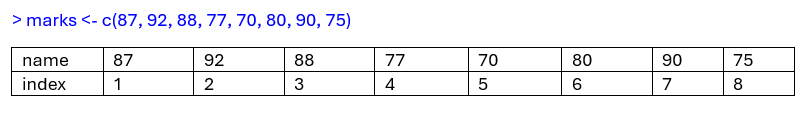
\includegraphics{img/03-index_numeric.png}
\caption{\label{fig:unnamed-chunk-67}Indexing for Numeric Vector}
\end{figure}

\begin{figure}
\centering
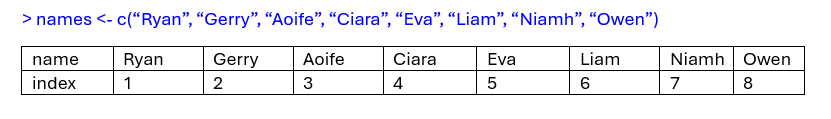
\includegraphics{img/03-index-character.png}
\caption{\label{fig:unnamed-chunk-68}Indexing for Character Vector}
\end{figure}

\begin{figure}
\centering
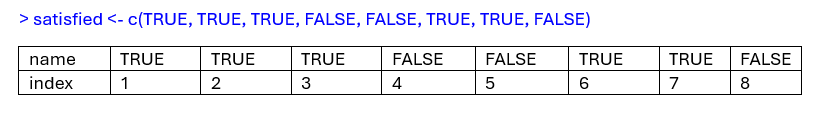
\includegraphics{img/03-index-logical.png}
\caption{\label{fig:unnamed-chunk-69}Indexing for Logical Vector}
\end{figure}

This property in vectors means we are capable of extracting specific items from a vector based on their position. If I wanted to extract the first item in my list, I can do this by using \textbf{\texttt{{[}{]}}} brackets:

\begin{Shaded}
\begin{Highlighting}[]
\NormalTok{rintro\_names[}\DecValTok{1}\NormalTok{]}
\end{Highlighting}
\end{Shaded}

\begin{verbatim}
## [1] "Gerry"
\end{verbatim}

Similarly, I could extract the 3rd element.

\begin{Shaded}
\begin{Highlighting}[]
\NormalTok{rintro\_marks[}\DecValTok{3}\NormalTok{]}
\end{Highlighting}
\end{Shaded}

\begin{verbatim}
## [1] 80
\end{verbatim}

Or I could extract the last element.

\begin{Shaded}
\begin{Highlighting}[]
\NormalTok{rintro\_satisfied[}\DecValTok{8}\NormalTok{]}
\end{Highlighting}
\end{Shaded}

\begin{verbatim}
## [1] FALSE
\end{verbatim}

This process is called subsetting. I am taking an original vector and taking a sub-portion of its original elements.

I can ask R even to subset several elements from my vector based on their position. Let's say I want to subset the 2nd, 4th, and 6th elements. I just need to use \textbf{\texttt{c()}} to tell R that I am subsetting several elements:

\begin{Shaded}
\begin{Highlighting}[]
\NormalTok{rintro\_names[}\FunctionTok{c}\NormalTok{(}\DecValTok{2}\NormalTok{, }\DecValTok{4}\NormalTok{, }\DecValTok{8}\NormalTok{)]}
\end{Highlighting}
\end{Shaded}

\begin{verbatim}
## [1] "Aoife" "Eva"   "Owen"
\end{verbatim}

\begin{Shaded}
\begin{Highlighting}[]
\NormalTok{rintro\_marks[}\FunctionTok{c}\NormalTok{(}\DecValTok{2}\NormalTok{, }\DecValTok{4}\NormalTok{, }\DecValTok{8}\NormalTok{)]}
\end{Highlighting}
\end{Shaded}

\begin{verbatim}
## [1] 65 77 71
\end{verbatim}

\begin{Shaded}
\begin{Highlighting}[]
\NormalTok{rintro\_satisfied[}\FunctionTok{c}\NormalTok{(}\DecValTok{2}\NormalTok{, }\DecValTok{4}\NormalTok{, }\DecValTok{8}\NormalTok{)]}
\end{Highlighting}
\end{Shaded}

\begin{verbatim}
## [1]  TRUE FALSE FALSE
\end{verbatim}

If the elements you are positioned right next to each other on a vector, you can use \textbf{\texttt{:}} as a shortcut:

\begin{Shaded}
\begin{Highlighting}[]
\NormalTok{rintro\_names[}\FunctionTok{c}\NormalTok{(}\DecValTok{1}\SpecialCharTok{:}\DecValTok{4}\NormalTok{)] }\CommentTok{\#this will extract the elements in index 1, 2, 3, 4}
\end{Highlighting}
\end{Shaded}

\begin{verbatim}
## [1] "Gerry" "Aoife" "Liam"  "Eva"
\end{verbatim}

It's important to know, however, that when you perform an operation on a vector or you subset it, it does not actually change the original vector. None of these following code will actually change rintro\_marks.

\begin{Shaded}
\begin{Highlighting}[]
\FunctionTok{sort}\NormalTok{(rintro\_marks, }\AttributeTok{decreasing =} \ConstantTok{TRUE}\NormalTok{)}

\NormalTok{[}\DecValTok{1}\NormalTok{] }\DecValTok{91} \DecValTok{90} \DecValTok{89} \DecValTok{88} \DecValTok{87} \DecValTok{87}

\FunctionTok{print}\NormalTok{(rintro\_marks)}
\NormalTok{[}\DecValTok{1}\NormalTok{] }\DecValTok{69} \DecValTok{65} \DecValTok{80} \DecValTok{77} \DecValTok{86} \DecValTok{88} \DecValTok{92} \DecValTok{71}

\NormalTok{rintro\_marks[}\FunctionTok{c}\NormalTok{(}\DecValTok{1}\NormalTok{, }\DecValTok{2}\NormalTok{, }\DecValTok{3}\NormalTok{)]}

\NormalTok{[}\DecValTok{1}\NormalTok{] }\DecValTok{87} \DecValTok{91} \DecValTok{87}

\FunctionTok{print}\NormalTok{(rintro\_marks)}
\NormalTok{[}\DecValTok{1}\NormalTok{] }\DecValTok{69} \DecValTok{65} \DecValTok{80} \DecValTok{77} \DecValTok{86} \DecValTok{88} \DecValTok{92} \DecValTok{71}
\end{Highlighting}
\end{Shaded}

You can see that neither the \textbf{\texttt{sort()}} function nor subsetting actually changed the original vector. They just outputted a result to the R console. If I wanted to actually save their results, then I would need to assign them to a variable label.

Here's how I would extract and save the top three exam marks:

\begin{Shaded}
\begin{Highlighting}[]
\NormalTok{marks\_sorted }\OtherTok{\textless{}{-}} \FunctionTok{sort}\NormalTok{(rintro\_marks, }\AttributeTok{decreasing =} \ConstantTok{TRUE}\NormalTok{)}

\NormalTok{marks\_top }\OtherTok{\textless{}{-}}\NormalTok{ marks\_sorted[}\FunctionTok{c}\NormalTok{(}\DecValTok{1}\SpecialCharTok{:}\DecValTok{3}\NormalTok{)]}

\FunctionTok{print}\NormalTok{(marks\_top)}
\end{Highlighting}
\end{Shaded}

\begin{verbatim}
## [1] 92 88 86
\end{verbatim}

\hypertarget{vectors---making-it-a-little-less-abstract.}{%
\subsubsection{Vectors - making it a little less abstract.}\label{vectors---making-it-a-little-less-abstract.}}

You might find the discussion of vectors, elements, and operations very abstract. I certainly did when I was learning R. While the list analogy is helpful, it only works for so long - there's another data structure called \textbf{\texttt{lists}} (we'll talk more about it next week). That confused me.

But what helped me understand vectors was the realization that a vector is simply a ``line of data.'' Let's say I was running a study and collected data on participants' age. When I open the Excel file, there will be a column called ``age'' with all the ages of my participants. That column is a vector of data with the variable label ``age.''

Creating that vector is the equivalent of creating a column in Excel:

\begin{Shaded}
\begin{Highlighting}[]
\NormalTok{age }\OtherTok{\textless{}{-}} \FunctionTok{c}\NormalTok{(}\DecValTok{18}\NormalTok{, }\DecValTok{23}\NormalTok{, }\DecValTok{43}\NormalTok{, }\DecValTok{23}\NormalTok{, }\DecValTok{44}\NormalTok{,}\DecValTok{32}\NormalTok{, }\DecValTok{56}\NormalTok{, }\DecValTok{67}\NormalTok{, }\DecValTok{32}\NormalTok{, }\DecValTok{23}\NormalTok{)}
\end{Highlighting}
\end{Shaded}

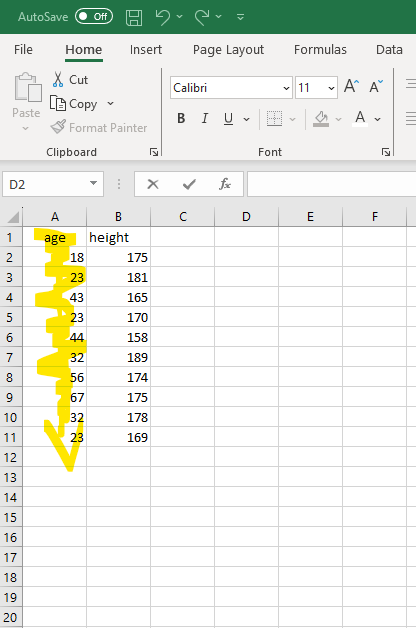
\includegraphics{img/03-column-vector.png}

Similarly, rows are also lines of data going horizontally. If I add data to columns in Excel to a dataset, I am creating a new row (line) of data. In R, this is the equivalent of doing this:

\begin{Shaded}
\begin{Highlighting}[]
\NormalTok{p11 }\OtherTok{\textless{}{-}} \FunctionTok{c}\NormalTok{(}\DecValTok{30}\NormalTok{, }\DecValTok{175}\NormalTok{)}
\end{Highlighting}
\end{Shaded}

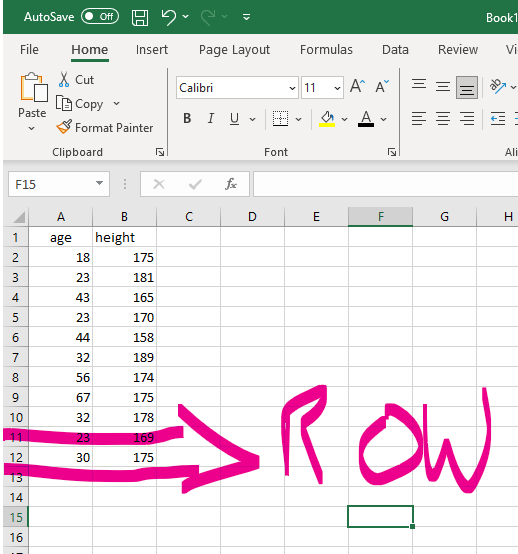
\includegraphics{img/03-row-vector.png}

So whenever you think of a vector, just remember that it refers to a line of data that would either be a column or a row.

So what happens when we combine different vectors (columns and rows) together? We create a \textbf{\texttt{data\ frame}}.

\hypertarget{data-frames}{%
\subsection{Data frames}\label{data-frames}}

A data frame is a rectangular data structure that is composed of rows and columns. A data frame in R is like a virtual table or a spreadsheet in Excel:

\begin{figure}
\centering
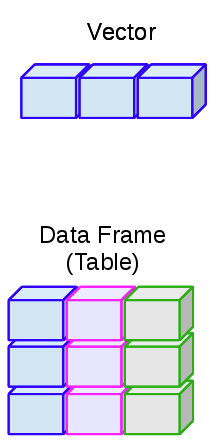
\includegraphics{img/03-dataframes_vectors.png}
\caption{\label{fig:unnamed-chunk-83}The relationship between data frames and vectors. The different colours in the data frame indicate they are composed of independent vectors}
\end{figure}

Data frames are an excellent way to store and manage data in R because they can store different types of data (e.g., character, numeric, integer) all within the same structure. Let's create such a data frame using the \textbf{\texttt{data.frame()}} function:

\begin{Shaded}
\begin{Highlighting}[]
\NormalTok{my\_df }\OtherTok{\textless{}{-}} \FunctionTok{data.frame}\NormalTok{(}
  \AttributeTok{Name =} \FunctionTok{c}\NormalTok{(}\StringTok{"Alice"}\NormalTok{, }\StringTok{"Bob"}\NormalTok{, }\StringTok{"Charlie"}\NormalTok{), }\CommentTok{\#a character vector}
  \AttributeTok{Age =} \FunctionTok{c}\NormalTok{(25L, 30L, 22L), }\CommentTok{\#an integer vector}
  \AttributeTok{Score =} \FunctionTok{c}\NormalTok{(}\FloatTok{95.65}\NormalTok{, }\FloatTok{88.12}\NormalTok{, }\FloatTok{75.33}\NormalTok{) }\CommentTok{\#a numeric vector}
\NormalTok{)}

\NormalTok{my\_df}
\end{Highlighting}
\end{Shaded}

\begin{verbatim}
##      Name Age Score
## 1   Alice  25 95.65
## 2     Bob  30 88.12
## 3 Charlie  22 75.33
\end{verbatim}

\hypertarget{selecting-data-from-a-data-frame}{%
\subsubsection{Selecting Data from a Data Frame}\label{selecting-data-from-a-data-frame}}

Once you have created or imported a data frame, you'll often need to access it and perform various tasks and analyses. Let's explore how to access data within a data frame effectively.

\hypertarget{selecting-columns}{%
\paragraph{Selecting Columns}\label{selecting-columns}}

Columns in a data frame represent different variables or attributes of your data. Often in data analysis, we want to select a specific column and then perform analyses on it. So how can we individually select columns? Well, in a data frame, every column has a name, similar to how each column in an Excel spreadsheet has a header. These column names enable you to access and manipulate specific columns or variables within your data frame.

We select columns based on their names via two tools:

The \textbf{\$} Notation: You can use a dollar sign (\$) followed by the column name to select \textbf{an individual column} in a data frame. For example, let's select the \textbf{\texttt{Name}} column in the \textbf{\texttt{my\_df}} data frame:

\begin{Shaded}
\begin{Highlighting}[]
\NormalTok{my\_df}\SpecialCharTok{$}\NormalTok{Name}
\end{Highlighting}
\end{Shaded}

\begin{verbatim}
## [1] "Alice"   "Bob"     "Charlie"
\end{verbatim}

\textbf{Square Brackets} \textbf{\texttt{{[}{]}}}: This is a similar approach to accessing elements from a vector. Inside the brackets, you can specify both the row and columns that you want to extract. The syntax for selecting rows and columns is: \textbf{\texttt{the\ dataframe{[}the\ rows\ we\ want,\ the\ columns\ we\ want{]}}}.

So if we wanted to access the ``Age'' column of \textbf{\texttt{my\_df}}, we could run the following code:

\begin{Shaded}
\begin{Highlighting}[]
\NormalTok{my\_df[, }\StringTok{"Age"}\NormalTok{]}
\end{Highlighting}
\end{Shaded}

\begin{verbatim}
## [1] 25 30 22
\end{verbatim}

You'll notice that we left the ``rows'' part empty in the square brackets. This tells R ``keep all the rows for this column.''

We can also use this approach to access multiple columns using the \textbf{\texttt{c()}} function:

\begin{Shaded}
\begin{Highlighting}[]
\NormalTok{my\_df[, }\FunctionTok{c}\NormalTok{(}\StringTok{"Age"}\NormalTok{, }\StringTok{"Score"}\NormalTok{)]}
\end{Highlighting}
\end{Shaded}

\begin{verbatim}
##   Age Score
## 1  25 95.65
## 2  30 88.12
## 3  22 75.33
\end{verbatim}

\hypertarget{selecting-rows}{%
\paragraph{Selecting Rows}\label{selecting-rows}}

Rows in a data frame represent individual observations or records. You can access rows using indexing, specifying the row number you want to retrieve, following the syntax: \textbf{\texttt{the\ dataframe{[}the\ rows\ we\ want,\ the\ columns\ we\ want{]}}}.

To get the first row of your data frame (\textbf{\texttt{my\_df}}), you can type the following:

\begin{Shaded}
\begin{Highlighting}[]
\NormalTok{my\_df[}\DecValTok{1}\NormalTok{, ]}
\end{Highlighting}
\end{Shaded}

\begin{verbatim}
##    Name Age Score
## 1 Alice  25 95.65
\end{verbatim}

This time I left the columns part blank; this tells R ``please keep all the columns for each row.''

To access the third row:

\begin{Shaded}
\begin{Highlighting}[]
\NormalTok{my\_df[}\DecValTok{3}\NormalTok{, ]}
\end{Highlighting}
\end{Shaded}

\begin{verbatim}
##      Name Age Score
## 3 Charlie  22 75.33
\end{verbatim}

If you want multiple rows, you can use the \textbf{\texttt{c()}} function to select multiple rows. Let's select the 1st and 3rd rows:

\begin{Shaded}
\begin{Highlighting}[]
\NormalTok{my\_df[}\FunctionTok{c}\NormalTok{(}\DecValTok{1}\NormalTok{, }\DecValTok{3}\NormalTok{), ]}
\end{Highlighting}
\end{Shaded}

\begin{verbatim}
##      Name Age Score
## 1   Alice  25 95.65
## 3 Charlie  22 75.33
\end{verbatim}

If you wanted to select a range of rows, you can use the : operator:

\begin{Shaded}
\begin{Highlighting}[]
\NormalTok{my\_df[}\DecValTok{2}\SpecialCharTok{:}\DecValTok{4}\NormalTok{, ]}
\end{Highlighting}
\end{Shaded}

\begin{verbatim}
##       Name Age Score
## 2      Bob  30 88.12
## 3  Charlie  22 75.33
## NA    <NA>  NA    NA
\end{verbatim}

These methods allow you to extract specific rows or subsets of rows from your data frame.

\hypertarget{selecting-rows-and-columns}{%
\paragraph{Selecting Rows and Columns}\label{selecting-rows-and-columns}}

We can also select both rows and columns using \textbf{\texttt{{[}{]}}} and our syntax: \textbf{\texttt{the\ dataframe{[}the\ rows\ we\ want,\ the\ columns\ we\ want{]}}}.

For example, we could select the first and third rows for the \textbf{\texttt{Age}} and \textbf{\texttt{Score}} columns:

\begin{Shaded}
\begin{Highlighting}[]
\NormalTok{my\_df[}\FunctionTok{c}\NormalTok{(}\DecValTok{1}\NormalTok{,}\DecValTok{3}\NormalTok{), }\FunctionTok{c}\NormalTok{(}\StringTok{"Age"}\NormalTok{, }\StringTok{"Score"}\NormalTok{)]}
\end{Highlighting}
\end{Shaded}

\begin{verbatim}
##   Age Score
## 1  25 95.65
## 3  22 75.33
\end{verbatim}

Similar to when we indexed vectors, this won't change the underlying data frame. To do that, we would need to assign the selection to a variable:

\begin{Shaded}
\begin{Highlighting}[]
\NormalTok{my\_df2 }\OtherTok{\textless{}{-}}\NormalTok{ my\_df[}\FunctionTok{c}\NormalTok{(}\DecValTok{1}\NormalTok{,}\DecValTok{3}\NormalTok{), }\FunctionTok{c}\NormalTok{(}\StringTok{"Age"}\NormalTok{, }\StringTok{"Score"}\NormalTok{)]}

\NormalTok{my\_df2}
\end{Highlighting}
\end{Shaded}

\begin{verbatim}
##   Age Score
## 1  25 95.65
## 3  22 75.33
\end{verbatim}

\hypertarget{adding-data-to-your-data-frame}{%
\subsubsection{Adding Data to your Data Frame}\label{adding-data-to-your-data-frame}}

\hypertarget{adding-columns}{%
\paragraph{Adding Columns}\label{adding-columns}}

You may often need to add new information to your data frame. For example, we might be interested in investigating the effect of \textbf{\texttt{Gender}} on the \textbf{\texttt{Score}} variable. The syntax for creating a new data frame is very straightforward:

\begin{Shaded}
\begin{Highlighting}[]
\NormalTok{existing\_df}\SpecialCharTok{$}\NormalTok{NewColumn }\OtherTok{\textless{}{-}} \FunctionTok{c}\NormalTok{(Value1, Value2, Value3)}
\end{Highlighting}
\end{Shaded}

Using this syntax, let's add a \textbf{\texttt{Gender}} column to our \textbf{\texttt{my\_df}} dataframe:.

\begin{Shaded}
\begin{Highlighting}[]
\NormalTok{my\_df}\SpecialCharTok{$}\NormalTok{Gender }\OtherTok{\textless{}{-}} \FunctionTok{c}\NormalTok{(}\StringTok{"Female"}\NormalTok{, }\StringTok{"Non{-}binary"}\NormalTok{, }\StringTok{"Male"}\NormalTok{)}

\CommentTok{\#let\textquotesingle{}s see if we have successfully added a new column in}

\NormalTok{my\_df}
\end{Highlighting}
\end{Shaded}

\begin{verbatim}
##      Name Age Score     Gender
## 1   Alice  25 95.65     Female
## 2     Bob  30 88.12 Non-binary
## 3 Charlie  22 75.33       Male
\end{verbatim}

Let's say I noticed I mixed up the genders, and that Bob is Male and Charlie is Non-Binary. Just like we can rewrite a variable, we can also rewrite a column using this approach:

\begin{Shaded}
\begin{Highlighting}[]
\NormalTok{my\_df}\SpecialCharTok{$}\NormalTok{Gender }\OtherTok{\textless{}{-}} \FunctionTok{c}\NormalTok{(}\StringTok{"Female"}\NormalTok{, }\StringTok{"Male"}\NormalTok{, }\StringTok{"Non{-}binary"}\NormalTok{)}

\CommentTok{\#let\textquotesingle{}s see if we have successfully rewritten the Gender Column}

\NormalTok{my\_df}
\end{Highlighting}
\end{Shaded}

\begin{verbatim}
##      Name Age Score     Gender
## 1   Alice  25 95.65     Female
## 2     Bob  30 88.12       Male
## 3 Charlie  22 75.33 Non-binary
\end{verbatim}

\hypertarget{adding-rows}{%
\paragraph{Adding Rows}\label{adding-rows}}

What about if we recruited more participants and wanted to add them to our data frame (it is pretty small at the moment!)? This is slightly more complicated, especially when we are dealing with data frames where each column (vector) is of a different data type.

What we need to do is actually create a new data frame that has the same columns as our original data frame. This new data frame will contain the new row(s) we want to add.

\begin{Shaded}
\begin{Highlighting}[]
\NormalTok{new\_row }\OtherTok{\textless{}{-}} \FunctionTok{data.frame}\NormalTok{(}\AttributeTok{Name =} \StringTok{"John"}\NormalTok{, }\AttributeTok{Age =} \DecValTok{30}\NormalTok{, }\AttributeTok{Score =} \FloatTok{77.34}\NormalTok{, }\AttributeTok{Gender =} \StringTok{"Male"}\NormalTok{)}
\end{Highlighting}
\end{Shaded}

Then we can use the \textbf{\texttt{rbind()}} function to add the new row to your original data frame. \textbf{\texttt{rbind}} takes in two data frames and combines them together. The syntax is as follows:

\begin{Shaded}
\begin{Highlighting}[]
\NormalTok{my\_df }\OtherTok{\textless{}{-}} \FunctionTok{rbind}\NormalTok{(my\_df, new\_row)}

\NormalTok{my\_df}
\end{Highlighting}
\end{Shaded}

\begin{verbatim}
##      Name Age Score     Gender
## 1   Alice  25 95.65     Female
## 2     Bob  30 88.12       Male
## 3 Charlie  22 75.33 Non-binary
## 4    John  30 77.34       Male
\end{verbatim}

\hypertarget{exercises-3}{%
\subsection{Exercises}\label{exercises-3}}

\begin{enumerate}
\def\labelenumi{\arabic{enumi}.}
\item
  Create one vector of each data type:

  \begin{enumerate}
  \def\labelenumii{\arabic{enumii}.}
  \item
    Create a character vector called \texttt{friends} with the name of 3 of your friends.
  \item
    Create an integer vector called \texttt{years} that describes the amount of years you have been friends (if it's less than 1 year, put 1).
  \item
    Create a numeric vector called \texttt{extra} with their extraversion scores (out of 5).
  \item
    Create a logical vector called \texttt{galway} that describes whether they live (\texttt{TRUE}) or don't live (\texttt{FALSE}) in Galway.
  \item
    Once you have created each vector, check whether it is the correct data type using the \texttt{class()} function.
  \end{enumerate}
\item
  Index the 2th, 4th, and 6th element for each of the following vectors.

\begin{Shaded}
\begin{Highlighting}[]
\NormalTok{vect1 }\OtherTok{\textless{}{-}} \FunctionTok{c}\NormalTok{(}\StringTok{"Not this"}\NormalTok{, }\StringTok{"This"}\NormalTok{, }\StringTok{"Not This"}\NormalTok{, }\StringTok{"This"}\NormalTok{, }\StringTok{"Not This"}\NormalTok{, }\StringTok{"This"}\NormalTok{)}

\NormalTok{vect2 }\OtherTok{\textless{}{-}} \FunctionTok{c}\NormalTok{(}\DecValTok{0}\NormalTok{, }\DecValTok{1}\NormalTok{, }\DecValTok{0}\NormalTok{, }\DecValTok{1}\NormalTok{, }\DecValTok{0}\NormalTok{, }\DecValTok{1}\NormalTok{)}

\NormalTok{vect3 }\OtherTok{\textless{}{-}} \FunctionTok{c}\NormalTok{(}\StringTok{"FALSE"}\NormalTok{, }\StringTok{"TRUE"}\NormalTok{, }\StringTok{"FALSE"}\NormalTok{, }\StringTok{"TRUE"}\NormalTok{, }\StringTok{"FALSE"}\NormalTok{)}
\end{Highlighting}
\end{Shaded}
\item
  How could we extract and save the bottom 3 results from the \texttt{rintro\_marks}vector? Bonus Points: Calculate the mean of both the top 3 marks and bottom 3 marks.
\item
  Write code that adds a column to the \texttt{my\_df} data frame called \texttt{Nationality}. The values for the column should be \texttt{"Irish"}, \texttt{"American"}, \texttt{"English"}, \texttt{"Irish"}.
\item
  Check whether that Nationality column has been successfully added by using the `\$` notation. The output should look like this.
\end{enumerate}

\begin{verbatim}
## [1] "English"  "American" "Irish"    "Irish"
\end{verbatim}

\begin{enumerate}
\def\labelenumi{\arabic{enumi}.}
\setcounter{enumi}{4}
\tightlist
\item
  What code could you write that would take the `my\_df` data frame and give you this output?
\end{enumerate}

\begin{verbatim}
##      Name Age Nationality
## 1   Alice  25     English
## 3 Charlie  22       Irish
\end{verbatim}

\begin{enumerate}
\def\labelenumi{\arabic{enumi}.}
\setcounter{enumi}{5}
\tightlist
\item
  Write code that adds a row to the \texttt{my\_df} data frame with your information for each of the columns (e.g., my data would be: \texttt{"Ryan"}, \texttt{30L}, \texttt{100}, \texttt{"Male"}). The \texttt{score} variable is a fake exam, so give yourself whatever score you want!
\end{enumerate}

\hypertarget{summary-1}{%
\section{Summary}\label{summary-1}}

That concludes this session. Well done, we did a lot of work today. We learned more about the relationship between the console and the script and how we need to be precise when writing commands. We introduced the different types of data that R stores and how those data types can be stored in single lines of data in vectors or combined together in a table in a \textbf{\texttt{data\ frame}}.

Don't feel like you need to have mastered or even remember all the material that we covered today. Even though these concepts are labeled as ``basic,'' that does not mean they are intuitive. It will take time for them to sink in, and that's normal. We'll drill these concepts a bit further next week. We'll also learn how to import \textbf{\texttt{data\ frames}}, which will set us up nicely for working with the type of data sets we see in Psychological research.

\hypertarget{glossary-1}{%
\section{Glossary}\label{glossary-1}}

This glossary defines key terms introduced in Chapter 3.

\begin{longtable}[]{@{}
  >{\raggedright\arraybackslash}p{(\columnwidth - 2\tabcolsep) * \real{0.2706}}
  >{\raggedright\arraybackslash}p{(\columnwidth - 2\tabcolsep) * \real{0.7294}}@{}}
\toprule\noalign{}
\begin{minipage}[b]{\linewidth}\raggedright
Term
\end{minipage} & \begin{minipage}[b]{\linewidth}\raggedright
Definition
\end{minipage} \\
\midrule\noalign{}
\endhead
\bottomrule\noalign{}
\endlastfoot
Assignment & The process of assigning a value to a variable using the assignment operator (\texttt{\textless{}-} or \texttt{=}). \\
Character & A data type representing text or strings of characters. \\
Data Frame & A two-dimensional data structure in R that resembles a table with rows and columns. It can store mixed data types. \\
Data Type & The classification of data values into categories, such as numeric, logical, integer, or character. \\
Element & An individual item or value within a data structure, such as a character in a vector. \\
Index & A numerical position or identifier used to access elements within a vector or other data structures. \\
Indexing & The process of selecting specific elements from a data structure using their index values. \\
Integer & A data type representing whole numbers without decimals. \\
Logical & A data type representing binary values (TRUE or FALSE), often used for conditions and logical operations. \\
Numeric & A data type representing numeric values, including real numbers and decimals. \\
Object & A fundamental data structure in R that can store data or values. Objects can include vectors, data frames, and more. \\
Subsetting & The technique of selecting a subset of elements from a data structure, such as a vector or data frame, based on specific criteria. \\
Variable & A named storage location in R that holds data or values. It can represent different types of information. \\
Vector & A one-dimensional data structure in R that can hold multiple elements of the same data type. \\
\end{longtable}

\hypertarget{variable-name-table}{%
\section{Variable Name Table}\label{variable-name-table}}

\begin{longtable}[]{@{}
  >{\raggedright\arraybackslash}p{(\columnwidth - 6\tabcolsep) * \real{0.3333}}
  >{\raggedright\arraybackslash}p{(\columnwidth - 6\tabcolsep) * \real{0.1414}}
  >{\raggedright\arraybackslash}p{(\columnwidth - 6\tabcolsep) * \real{0.2626}}
  >{\raggedright\arraybackslash}p{(\columnwidth - 6\tabcolsep) * \real{0.2626}}@{}}
\toprule\noalign{}
\begin{minipage}[b]{\linewidth}\raggedright
Rule
\end{minipage} & \begin{minipage}[b]{\linewidth}\raggedright
Type
\end{minipage} & \begin{minipage}[b]{\linewidth}\raggedright
Incorrect Example
\end{minipage} & \begin{minipage}[b]{\linewidth}\raggedright
Correct Example
\end{minipage} \\
\midrule\noalign{}
\endhead
\bottomrule\noalign{}
\endlastfoot
Variable names can only contain uppercase alphabetic characters A-Z, lowercase a-z, numeric characters 0-9, periods ., and underscores \_. & Strict & 1st\_name & first\_name \\
Variable names must begin with a letter or a period. & Strict & \_1stname & .firstname \\
Avoid using spaces in variable names. & Strict & my name & my\_name \\
Variable names are case-sensitive. & Strict & my\_name == my\_Name & my\_Name == my\_Name \\
Variable names cannot include special words reserved by R. & Strict & print & to\_print \\
Choose informative variable names that clearly describe the information they represent. & Recommended & money & income \\
Opt for short variable names when possible. & Recommended & date\_of\_birth & dob \\
Prioritize clarity over brevity. & Recommended & tem & total\_exam\_marks \\
Avoid starting variable names with a capital letter. & Recommended & FirstName & firstName \\
Choose a consistent naming style and stick to it. & Recommended & myName, last\_Name & my\_name, last\_name or myName and lastName \\
\end{longtable}

\hypertarget{programming2}{%
\chapter{\texorpdfstring{\textbf{R Programming (Part II)}}{R Programming (Part II)}}\label{programming2}}

Today, we are going to build upon the foundational concepts introduced last week and delve deeper into the world of R programming.

By the end of this session, you should be capable of the following:

\begin{itemize}
\item
  Understanding the logic of functions, including how and why they are created.
\item
  Creating the ``factor'' data type and the list data structure.
\item
  Being capable of enhancing your RStudio experience by installing and loading packages.
\item
  Importing a dataset into R using both code and button-click interfaces from CSV and SPSS files.
\item
  Exporting data to CSV and SPSS files.
\end{itemize}

\hypertarget{functions}{%
\section{Functions}\label{functions}}

In the previous two sessions, we have used several functions including: \textbf{\texttt{print()}}, \textbf{\texttt{head()}}, \textbf{\texttt{View()}}, \textbf{\texttt{mean()}}, \textbf{\texttt{sd()}}, \textbf{\texttt{summary()}}, \textbf{\texttt{aggregate()}}, \textbf{\texttt{plot()}}, \textbf{\texttt{pdf()}}, \textbf{\texttt{t.test()}}, \textbf{\texttt{class()}}, and \textbf{\texttt{c()}}. Each of these functions has served a particular purpose. All of them have taken in an input object (e.g., a variable, data type, and/or data structure), performed some operation on it, and produced some output.

But we haven't really talked about what functions actually are. I have told you they are similar to verbs in that they are ``words'' that do things. This makes them sound like some magical words.

You might assume that being good at programming is about learning as many functions as you can, and learning in detail what they can do, so that whenever you face a challenging situation in R, you know what tool to use.

There is some truth to this. You will inevitably learn more functions as you get better and more comfortable with R. This will make you more adept at using them. But what actually predicts becoming good at programming is your ability to understand the logic of functions and how they are created. If you grasp that, you'll be able to learn them quicker, use them more effectively, and even create your own functions.

This final point is critical. You can create your own functions. Let's create our own function to demonstrate what functions actually are.

\hypertarget{the-syntax-for-creating-a-function}{%
\subsection{The Syntax for Creating a Function}\label{the-syntax-for-creating-a-function}}

Functions are somewhat similar to variables. We create variable names as labels for information. That way when we want to access that information or perform operations on it we can use the variable name rather than recreating the information in R again.

Similarly, functions are like labels for code. We come up with a name for a function (e.g., \textbf{\texttt{mean()}}) and we assign code instructions to that function. So when we call a function, we can give it information (e.g., variables), and it will take information and run that code on it. This way we don't have to write out code instructions over and over again - we can just call the function. This increases the scalability of our code.

The syntax for creating a function looks like this:

\begin{Shaded}
\begin{Highlighting}[]
\NormalTok{my\_function }\OtherTok{\textless{}{-}} \ControlFlowTok{function}\NormalTok{(argument) \{}
\NormalTok{  instruction\_1}
\NormalTok{  instructions\_2}
\NormalTok{  ....}
\NormalTok{  instruction\_n}
  \FunctionTok{return}\NormalTok{(output)}
\NormalTok{\}}
\end{Highlighting}
\end{Shaded}

What's going on here?

\begin{enumerate}
\def\labelenumi{\arabic{enumi}.}
\item
  First, we created a name, \textbf{\texttt{my\_function}}, and used the assignment operator \textbf{\texttt{\textless{}-}} to tell R we are going to be storing some piece of information to that name.
\item
  Then, we wrote \textbf{\texttt{function()}} to tell R that we are going to be creating a function and storing it to our name \textbf{\texttt{my\_function}}. Inside \textbf{\texttt{function()}}, we specified an \textbf{\texttt{argument}}, which is just a fancy word for \textbf{\texttt{input}}.
\item
  Inside the curly brackets \textbf{\texttt{\{\}}}, we write the code for \textbf{\texttt{my\_function}}. This code comprises instructions (i.e., operations) that R will execute on our argument (i.e., input). We could have 1 instruction here, or we could have several hundred lines of instructions. That depends on the complexity of the function we are creating.
\item
  We want the function to provide us with some output information. To ensure that it does that, we tell R to \textbf{\texttt{return()}} the information (\textbf{\texttt{output}}) that we want.
\end{enumerate}

\hypertarget{creating-a-simple-function-1-argument}{%
\subsection{Creating a Simple Function (1-Argument)}\label{creating-a-simple-function-1-argument}}

It may come as a shock to you to learn that I am not much of a chef. One of the reasons I'm not a chef is my irritation with reading recipes that include instructions like ``1 cup,'' ``10 ounces,'' or ``17 eagle feet,'' or require preheating the oven to ``1000 degrees Fahrenheit.'' What I could really use is a function that would help me convert those values automatically. Let's take the cup example. Let's create a function that will take in the number of cups we need and convert that to grams.

To do this, let's create a function called \textbf{\texttt{cups\_to\_grams}} (note: the naming conventions for functions are similar to the naming conventions for variables. The main rule is that your function name should describe the action it is carrying out.)

\begin{Shaded}
\begin{Highlighting}[]
\NormalTok{cups\_to\_grams }\OtherTok{\textless{}{-}} \ControlFlowTok{function}\NormalTok{(cups) \{}
  
\NormalTok{\}}
\end{Highlighting}
\end{Shaded}

Inside the \textbf{\texttt{function()}}, I have given it the argument \textbf{\texttt{cups}}. In this scenario, \textbf{\texttt{cups}} acts as a placeholder variable. Inside the function, we are going to write instructions on what to do with that variable. But we have not yet defined what that variable is yet. We do that when we use the function. So don't worry about that for now.

Now inside our function (i.e., inside the \textbf{\texttt{\{\}}}), we need to write instructions to enable R to convert cups to grams. When I googled this, several different answers popped up. But I am just going to follow the first website I found which said: ``According to the metric system, there are 250 grams in 1 cup.''

Let's write that instruction inside our function. We are going to save the result of that calculation to a variable called \textbf{\texttt{grams}}.

\begin{Shaded}
\begin{Highlighting}[]
\NormalTok{cups\_to\_grams }\OtherTok{\textless{}{-}} \ControlFlowTok{function}\NormalTok{(cups) \{}
\NormalTok{  grams }\OtherTok{\textless{}{-}}\NormalTok{ cups }\SpecialCharTok{*} \DecValTok{250}
\NormalTok{\}}
\end{Highlighting}
\end{Shaded}

Now we are nearly done. But if we want R to provide us with the result of this function, we need to ask it to \textbf{\texttt{return()}} it to us. We can do that easily by:

\begin{Shaded}
\begin{Highlighting}[]
\NormalTok{cups\_to\_grams }\OtherTok{\textless{}{-}} \ControlFlowTok{function}\NormalTok{(cups) \{}
\NormalTok{  grams }\OtherTok{\textless{}{-}}\NormalTok{ cups }\SpecialCharTok{*} \DecValTok{250}
  \FunctionTok{return}\NormalTok{(grams)}
\NormalTok{\}}
\end{Highlighting}
\end{Shaded}

There we have it, we have created our first function! Now let's see if it works. In programming lingo, we say that we \textbf{\texttt{call}} a function when we use it. To call \textbf{\texttt{cups\_to\_grams}} it is the same process as the other functions we have used, we type out the name and then we insert our input inside the parentheses.

\begin{Shaded}
\begin{Highlighting}[]
\FunctionTok{cups\_to\_grams}\NormalTok{(}\AttributeTok{cups =} \DecValTok{1}\NormalTok{)}
\end{Highlighting}
\end{Shaded}

\begin{verbatim}
## [1] 250
\end{verbatim}

It works! We can see here what I mean that \textbf{\texttt{cups}} is a placeholder variable. We want our function to be generalizable, so we don't tell it ahead of time what \textbf{\texttt{cups}} equals. All it knows is that it will receive some information that will equate to cups, and then it will multiply that information by 250.

This enables us to call our function several times with several different values.

\begin{Shaded}
\begin{Highlighting}[]
\FunctionTok{cups\_to\_grams}\NormalTok{(}\AttributeTok{cups =} \DecValTok{4}\NormalTok{)}
\end{Highlighting}
\end{Shaded}

\begin{verbatim}
## [1] 1000
\end{verbatim}

\begin{Shaded}
\begin{Highlighting}[]
\FunctionTok{cups\_to\_grams}\NormalTok{(}\AttributeTok{cups =} \DecValTok{2}\NormalTok{)}
\end{Highlighting}
\end{Shaded}

\begin{verbatim}
## [1] 500
\end{verbatim}

\begin{Shaded}
\begin{Highlighting}[]
\FunctionTok{cups\_to\_grams}\NormalTok{(}\AttributeTok{cups =} \FloatTok{1.5}\NormalTok{)}
\end{Highlighting}
\end{Shaded}

\begin{verbatim}
## [1] 375
\end{verbatim}

\begin{Shaded}
\begin{Highlighting}[]
\FunctionTok{cups\_to\_grams}\NormalTok{(}\AttributeTok{cups =}\NormalTok{ 5L)}
\end{Highlighting}
\end{Shaded}

\begin{verbatim}
## [1] 1250
\end{verbatim}

We can also define what \texttt{cups} is outside of the function.

\begin{Shaded}
\begin{Highlighting}[]
\NormalTok{cups }\OtherTok{=} \DecValTok{2}
\FunctionTok{cups\_to\_grams}\NormalTok{(cups)}
\end{Highlighting}
\end{Shaded}

\begin{verbatim}
## [1] 500
\end{verbatim}

This is an example of a 1-argument function, as it only takes in 1 input. But we can also create functions that have multiple arguments.

\hypertarget{creating-a-multi-argument-function}{%
\subsection{Creating a Multi-Argument Function}\label{creating-a-multi-argument-function}}

You might have noticed previously that sometimes we put additional information inside functions, like \textbf{\texttt{paired\ =\ TRUE}} in \textbf{\texttt{t.test()}}, or \textbf{\texttt{descending\ =\ FALSE}} in \textbf{\texttt{sort()}}. This additional information represents other arguments that we can insert inside a function.

The process for creating a multi-argument function is the same as for a single-argument function. Let's create a function called \textbf{\texttt{calculate\_z\_score}} that calculates the z-score of a value.

\begin{Shaded}
\begin{Highlighting}[]
\NormalTok{calculate\_z\_score }\OtherTok{\textless{}{-}} \ControlFlowTok{function}\NormalTok{(x, mean\_val, sd\_val) \{}
  \CommentTok{\# Calculate the z{-}score}
\NormalTok{  z\_score }\OtherTok{\textless{}{-}}\NormalTok{ (x }\SpecialCharTok{{-}}\NormalTok{ mean\_val) }\SpecialCharTok{/}\NormalTok{ sd\_val}
  
  \CommentTok{\# Return the z{-}score}
  \FunctionTok{return}\NormalTok{(z\_score)}
\NormalTok{\}}
\end{Highlighting}
\end{Shaded}

In this function:

\begin{itemize}
\item
  \textbf{\texttt{x}} is the value for which we want to calculate the z-score.
\item
  \textbf{\texttt{mean\_val}} is the mean score of the variable within our dataset.
\item
  \textbf{\texttt{sd\_val}} is the standard deviation of the variable within our dataset.
\end{itemize}

Inside the function, we calculate the z-score using the formula \textbf{\texttt{(x\ -\ mean\_val)\ /\ sd\_val}}. The calculated z-score is returned as the output of the function.

Just like before, none of the placeholder arguments (\textbf{\texttt{x}}, \textbf{\texttt{mean\_val}}, and \textbf{\texttt{sd\_val}}) are defined beforehand. We will define them in our script or when we call our function.

To test this function, let's use an example of an IQ score since we know the population mean (100) and standard deviation (15). Let's see what the z-score is for someone with an IQ of 130.

\begin{Shaded}
\begin{Highlighting}[]
\FunctionTok{calculate\_z\_score}\NormalTok{(}\AttributeTok{x =} \DecValTok{130}\NormalTok{, }\AttributeTok{mean\_val =} \DecValTok{100}\NormalTok{, }\AttributeTok{sd\_val =} \DecValTok{15}\NormalTok{)}
\end{Highlighting}
\end{Shaded}

\begin{verbatim}
## [1] 2
\end{verbatim}

Just as we would expect, a person with an IQ of 130 is 2 standard deviations away from the mean. This shows that our function is working as expected.

What if we had a vector of IQ scores? Could we use our function to calculate the z-score of each element in our vector? Absolutely!

\begin{Shaded}
\begin{Highlighting}[]
\FunctionTok{calculate\_z\_score}\NormalTok{(}\AttributeTok{x =} \FunctionTok{c}\NormalTok{(}\DecValTok{100}\NormalTok{, }\DecValTok{130}\NormalTok{, }\DecValTok{85}\NormalTok{), }\AttributeTok{mean\_val =} \DecValTok{100}\NormalTok{, }\AttributeTok{sd\_val =} \DecValTok{15}\NormalTok{)}
\end{Highlighting}
\end{Shaded}

\begin{verbatim}
## [1]  0  2 -1
\end{verbatim}

Sticking with this example, let's say we had a data frame with participant IDs, their age, and their IQ scores. We could feed the vector \textbf{\texttt{iq\_scores}} into our \textbf{\texttt{calculate\_z\_score}} function, calculate their z-scores, and create a column based on those scores.

\begin{Shaded}
\begin{Highlighting}[]
\CommentTok{\#first let\textquotesingle{}s make that data frame}

\NormalTok{iq\_df }\OtherTok{\textless{}{-}} \FunctionTok{data.frame}\NormalTok{(}
  \AttributeTok{ID =} \FunctionTok{c}\NormalTok{(}\DecValTok{1}\NormalTok{, }\DecValTok{2}\NormalTok{, }\DecValTok{3}\NormalTok{, }\DecValTok{4}\NormalTok{, }\DecValTok{5}\NormalTok{, }\DecValTok{6}\NormalTok{, }\DecValTok{7}\NormalTok{, }\DecValTok{8}\NormalTok{),}
  \AttributeTok{age =} \FunctionTok{c}\NormalTok{(}\DecValTok{22}\NormalTok{, }\DecValTok{30}\NormalTok{, }\DecValTok{41}\NormalTok{, }\DecValTok{45}\NormalTok{, }\DecValTok{18}\NormalTok{, }\DecValTok{21}\NormalTok{, }\DecValTok{23}\NormalTok{, }\DecValTok{45}\NormalTok{),}
  \AttributeTok{iq =} \FunctionTok{c}\NormalTok{(}\DecValTok{100}\NormalTok{, }\DecValTok{123}\NormalTok{, }\DecValTok{111}\NormalTok{, }\DecValTok{130}\NormalTok{, }\DecValTok{90}\NormalTok{, }\DecValTok{102}\NormalTok{, }\DecValTok{88}\NormalTok{, }\DecValTok{109}\NormalTok{)}
\NormalTok{)}

\CommentTok{\#now let\textquotesingle{}s feed that IQ vector into our function and save it to a variable}

\NormalTok{iq\_z\_scores }\OtherTok{\textless{}{-}}  \FunctionTok{calculate\_z\_score}\NormalTok{(}\AttributeTok{x =}\NormalTok{ iq\_df}\SpecialCharTok{$}\NormalTok{iq, }\AttributeTok{mean\_val =} \DecValTok{100}\NormalTok{, }\AttributeTok{sd\_val =} \DecValTok{15}\NormalTok{) }\CommentTok{\#this will create a vector called iq\_z\_scores that is the output of our calculate\_z\_score}


\CommentTok{\#if we want to add that column, we use the syntax }

\CommentTok{\#dataframe$newColumnName \textless{}{-} \#new\_vector}

\NormalTok{iq\_df}\SpecialCharTok{$}\NormalTok{iq\_z\_scores }\OtherTok{\textless{}{-}}\NormalTok{ iq\_z\_scores}


\CommentTok{\#now let\textquotesingle{}s check our data frame}

\FunctionTok{head}\NormalTok{(iq\_df)}
\end{Highlighting}
\end{Shaded}

\begin{verbatim}
##   ID age  iq iq_z_scores
## 1  1  22 100   0.0000000
## 2  2  30 123   1.5333333
## 3  3  41 111   0.7333333
## 4  4  45 130   2.0000000
## 5  5  18  90  -0.6666667
## 6  6  21 102   0.1333333
\end{verbatim}

While \textbf{\texttt{calculate\_z\_score}} is pretty handy, it's not perfect. It requires us to calculate the mean and standard deviation functions separately and then feed that into our function. That's okay if we are dealing with variables that have a known mean and standard deviation. Outside of those examples, we would need to do some extra work. But one of the virtues about functions is that it enables us to be lazy - we want to write functions that will automate boring tasks for us. So how could we improve this function? Well luckily, we can include functions inside functions.

\hypertarget{functions-inside-functions}{%
\subsection{Functions inside Functions}\label{functions-inside-functions}}

Let's say that we add a column in our \textbf{\texttt{iq\_df}} dataframe that contains participants' mean scores on Beck's Depression Inventory. We'll call this column \textbf{\texttt{total\_depression\_beck}}.

\begin{Shaded}
\begin{Highlighting}[]
\NormalTok{iq\_df}\SpecialCharTok{$}\NormalTok{total\_depression\_beck }\OtherTok{\textless{}{-}} \FunctionTok{c}\NormalTok{(}\DecValTok{32}\NormalTok{, }\DecValTok{36}\NormalTok{, }\DecValTok{34}\NormalTok{, }\DecValTok{46}\NormalTok{, }
                                \DecValTok{30}\NormalTok{, }\DecValTok{53}\NormalTok{, }\DecValTok{40}\NormalTok{, }\DecValTok{15}\NormalTok{) }\CommentTok{\#adds the mean\_depression beck vector to our dataframe}

\FunctionTok{head}\NormalTok{(iq\_df) }\CommentTok{\#check to see if it was added correctly.}
\end{Highlighting}
\end{Shaded}

\begin{verbatim}
##   ID age  iq iq_z_scores total_depression_beck
## 1  1  22 100   0.0000000                    32
## 2  2  30 123   1.5333333                    36
## 3  3  41 111   0.7333333                    34
## 4  4  45 130   2.0000000                    46
## 5  5  18  90  -0.6666667                    30
## 6  6  21 102   0.1333333                    53
\end{verbatim}

Since we do not know the mean and standard deviation of the Beck Inventory, we will need to calculate them using the \textbf{\texttt{mean()}} and \textbf{\texttt{sd()}} functions. Luckily, we can use those functions within \textbf{\texttt{calculate\_z\_score}} to enable this for us. Let's add this to our function and call it.

\begin{Shaded}
\begin{Highlighting}[]
\NormalTok{calculate\_z\_score }\OtherTok{\textless{}{-}} \ControlFlowTok{function}\NormalTok{(x) \{}
  \CommentTok{\# Calculate the z{-}score}
\NormalTok{  z\_score }\OtherTok{\textless{}{-}}\NormalTok{ (x }\SpecialCharTok{{-}}\NormalTok{ mean\_val) }\SpecialCharTok{/}\NormalTok{ sd\_val}
\NormalTok{  mean\_val }\OtherTok{\textless{}{-}} \FunctionTok{mean}\NormalTok{(x)}
\NormalTok{  sd\_val }\OtherTok{\textless{}{-}} \FunctionTok{sd}\NormalTok{(x)}
  
  \CommentTok{\# Return the z{-}score}
  \FunctionTok{return}\NormalTok{(z\_score)}
\NormalTok{\}}

\FunctionTok{calculate\_z\_score}\NormalTok{(}\AttributeTok{x =} \FunctionTok{c}\NormalTok{(}\DecValTok{100}\NormalTok{, }\DecValTok{90}\NormalTok{, }\DecValTok{110}\NormalTok{))}
\end{Highlighting}
\end{Shaded}

\begin{verbatim}
## Error in calculate_z_score(x = c(100, 90, 110)): object 'mean_val' not found
\end{verbatim}

Uh-oh! Why is it telling us that the object \textbf{\texttt{mean\_val}} was not found? The reason for this is that the order of your code within a function matters. The order of your code is the order in which R will compute that instruction. Currently, I have asked R to compute \textbf{\texttt{z\_score}} before defining what \textbf{\texttt{mean\_val}} or \textbf{\texttt{sd\_val}} are.

So when R sees \textbf{\texttt{mean\_val}}, it looks everywhere for what that value could mean, doesn't find anything, and then panics and stops working. Again, humans have a theory of mind, so we would assume that we could provide this information. But R needs to do everything literally step-by-step.

To rectify this, we just need to fix the order of our instructions inside R.

\begin{Shaded}
\begin{Highlighting}[]
\NormalTok{calculate\_z\_score }\OtherTok{\textless{}{-}} \ControlFlowTok{function}\NormalTok{(x, mean\_val, sd\_val) \{}
  \CommentTok{\#compute mean\_val, and sd\_val first}
\NormalTok{  mean\_val }\OtherTok{\textless{}{-}} \FunctionTok{mean}\NormalTok{(x)}
\NormalTok{  sd\_val }\OtherTok{\textless{}{-}} \FunctionTok{sd}\NormalTok{(x)}
  
\NormalTok{  z\_score }\OtherTok{\textless{}{-}}\NormalTok{ (x }\SpecialCharTok{{-}}\NormalTok{ mean\_val) }\SpecialCharTok{/}\NormalTok{ sd\_val}
  
  \CommentTok{\# Return the z{-}score}
  \FunctionTok{return}\NormalTok{(z\_score)}
\NormalTok{\}}

\FunctionTok{calculate\_z\_score}\NormalTok{(}\AttributeTok{x =}\NormalTok{ iq\_df}\SpecialCharTok{$}\NormalTok{total\_depression\_beck)}
\end{Highlighting}
\end{Shaded}

\begin{verbatim}
## [1] -0.33044366  0.02202958 -0.15420704  0.90321267 -0.50668028  1.52004083
## [7]  0.37450281 -1.82845491
\end{verbatim}

Wahey, it worked! Try to add the z-scores for the \textbf{\texttt{total\_depression\_beck}} to the dataframe yourself (look at the end of the previous subsection for advice on how if you are stuck).

\hypertarget{returning-multiple-objects-from-a-function}{%
\subsection{Returning Multiple Objects from a Function}\label{returning-multiple-objects-from-a-function}}

What if we wanted to return not only the \texttt{z\_score} variable from calculate\_z\_score, but also \texttt{mean\_val} and \texttt{sd\_val} as well?

Luckily, we can also tell our functions to return multiple different objects at the same time. We can do this by using lists.

We will discuss lists in more detail later in this chapter. For now, all you need to know is that lists are versatile data structures in R that can hold elements of different types. We can create a list within a function, populate it with the values we want to return, and then return the list itself.

We can create a variable within our function that is a list containing all the information we want to return. But since this changes the nature of the function, we are going to change its name to: `calculate\_mean\_sd\_z`

\begin{Shaded}
\begin{Highlighting}[]
\NormalTok{calculate\_mean\_sd\_z }\OtherTok{\textless{}{-}} \ControlFlowTok{function}\NormalTok{(x, mean\_val, sd\_val) \{}
  \CommentTok{\#compute mean\_val, and sd\_val first}
\NormalTok{  mean\_val }\OtherTok{\textless{}{-}} \FunctionTok{mean}\NormalTok{(x)}
\NormalTok{  sd\_val }\OtherTok{\textless{}{-}} \FunctionTok{sd}\NormalTok{(x)}
  
\NormalTok{  z\_score }\OtherTok{\textless{}{-}}\NormalTok{ (x }\SpecialCharTok{{-}}\NormalTok{ mean\_val) }\SpecialCharTok{/}\NormalTok{ sd\_val}
  
\NormalTok{  results }\OtherTok{\textless{}{-}} \FunctionTok{list}\NormalTok{(z\_score, mean\_val, sd\_val)}
  
  \CommentTok{\# Return the z{-}score}
  \FunctionTok{return}\NormalTok{(results)}
\NormalTok{\}}

\FunctionTok{calculate\_mean\_sd\_z}\NormalTok{(iq\_df}\SpecialCharTok{$}\NormalTok{total\_depression\_beck)}
\end{Highlighting}
\end{Shaded}

\begin{verbatim}
## [[1]]
## [1] -0.33044366  0.02202958 -0.15420704  0.90321267 -0.50668028  1.52004083
## [7]  0.37450281 -1.82845491
## 
## [[2]]
## [1] 35.75
## 
## [[3]]
## [1] 11.34838
\end{verbatim}

This produces the results that we want, but the output leaves a lot to be desired. If someone else was calling our function, but was not aware of the instructions inside it, they might not know what each value from the output corresponds to. We can correct this by using the following syntax inside the list to label each value: \texttt{name\_of\_value\ =\ value}

\begin{Shaded}
\begin{Highlighting}[]
\NormalTok{calculate\_mean\_sd\_z }\OtherTok{\textless{}{-}} \ControlFlowTok{function}\NormalTok{(x, mean\_val, sd\_val) \{}
  \CommentTok{\#compute mean\_val, and sd\_val first}
\NormalTok{  mean\_val }\OtherTok{\textless{}{-}} \FunctionTok{mean}\NormalTok{(x)}
\NormalTok{  sd\_val }\OtherTok{\textless{}{-}} \FunctionTok{sd}\NormalTok{(x)}
  
\NormalTok{  z\_score }\OtherTok{\textless{}{-}}\NormalTok{ (x }\SpecialCharTok{{-}}\NormalTok{ mean\_val) }\SpecialCharTok{/}\NormalTok{ sd\_val}
  
\NormalTok{  results }\OtherTok{\textless{}{-}} \FunctionTok{list}\NormalTok{(}\AttributeTok{z =}\NormalTok{ z\_score, }\AttributeTok{mean =}\NormalTok{ mean\_val, }\AttributeTok{sd =}\NormalTok{ sd\_val)}
  
  \CommentTok{\# Return the z{-}score}
  \FunctionTok{return}\NormalTok{(results)}
\NormalTok{\}}

\FunctionTok{calculate\_mean\_sd\_z}\NormalTok{(iq\_df}\SpecialCharTok{$}\NormalTok{total\_depression\_beck)}
\end{Highlighting}
\end{Shaded}

\begin{verbatim}
## $z
## [1] -0.33044366  0.02202958 -0.15420704  0.90321267 -0.50668028  1.52004083
## [7]  0.37450281 -1.82845491
## 
## $mean
## [1] 35.75
## 
## $sd
## [1] 11.34838
\end{verbatim}

Now if we wanted to extract certain features from the function, we can use the `\$` operator.

\begin{Shaded}
\begin{Highlighting}[]
\NormalTok{scores }\OtherTok{\textless{}{-}}  \FunctionTok{calculate\_mean\_sd\_z}\NormalTok{(iq\_df}\SpecialCharTok{$}\NormalTok{total\_depression\_beck)}

\NormalTok{scores}\SpecialCharTok{$}\NormalTok{mean}
\end{Highlighting}
\end{Shaded}

\begin{verbatim}
## [1] 35.75
\end{verbatim}

\begin{Shaded}
\begin{Highlighting}[]
\NormalTok{scores}\SpecialCharTok{$}\NormalTok{sd}
\end{Highlighting}
\end{Shaded}

\begin{verbatim}
## [1] 11.34838
\end{verbatim}

\begin{Shaded}
\begin{Highlighting}[]
\NormalTok{scores}\SpecialCharTok{$}\NormalTok{z}
\end{Highlighting}
\end{Shaded}

\begin{verbatim}
## [1] -0.33044366  0.02202958 -0.15420704  0.90321267 -0.50668028  1.52004083
## [7]  0.37450281 -1.82845491
\end{verbatim}

\hypertarget{some-important-features-about-functions}{%
\subsection{Some Important Features about Functions}\label{some-important-features-about-functions}}

There are some important features about functions that you should know. Namely, the difference between Global and Local Variables and the ability to set and override Default Arguments.

\hypertarget{global-vs-local-variables}{%
\subsubsection{Global vs Local Variables}\label{global-vs-local-variables}}

It is important to note that R treats variables you define in a function differently than variables you define outside of a function. Any variable you define within a function will only exist within the scope of that function. Variables defined in a function are called local variables whereas variables defined outside of a function are called global variables.

\begin{Shaded}
\begin{Highlighting}[]
\NormalTok{num1 }\OtherTok{\textless{}{-}} \DecValTok{20} \CommentTok{\#this is a global variable}

\NormalTok{local\_global }\OtherTok{\textless{}{-}} \ControlFlowTok{function}\NormalTok{() \{}
\NormalTok{  num1 }\OtherTok{\textless{}{-}} \DecValTok{10}\CommentTok{\#this is a local variable}
  \FunctionTok{print}\NormalTok{(num1)  }\CommentTok{\# This will print 10}
\NormalTok{\}}

\FunctionTok{local\_global}\NormalTok{()}
\end{Highlighting}
\end{Shaded}

\begin{verbatim}
## [1] 10
\end{verbatim}

\begin{Shaded}
\begin{Highlighting}[]
\FunctionTok{print}\NormalTok{(num1)  }\CommentTok{\# Error: object \textquotesingle{}local\_var\textquotesingle{} not found}
\end{Highlighting}
\end{Shaded}

\begin{verbatim}
## [1] 20
\end{verbatim}

We start this code chunk by assigning the value 20 to the variable \texttt{num1}. This is a global variable, it will exist across our R environment unless we change it to a different value.

Within the \texttt{local\_global()} function, we create another variable called \texttt{num1} and assign it the value of 10. But this is an example of a local variable, as it only exists inside of our function. When we run our function, it will print out 10, but the function will not change the global value of the variable.

\hypertarget{default-arguments}{%
\subsubsection{Default Arguments}\label{default-arguments}}

In R, functions can have default arguments, which are pre-defined values assigned to arguments in the function definition. Default arguments allow functions to be called with fewer arguments than specified in the function definition, as the default values are used when the arguments are not explicitly provided.

\hypertarget{syntax-for-default-arguments}{%
\subsubsection{Syntax for Default Arguments}\label{syntax-for-default-arguments}}

The syntax for defining default arguments in R functions is straightforward. When defining the function, you can assign default values to specific arguments using the \textbf{\texttt{argument\ =\ default\_value}} format.

Imagine I wanted to write a function that greeted someone. I could write the following function, \textbf{\texttt{greet}}:

\begin{Shaded}
\begin{Highlighting}[]
\CommentTok{\# Function with default argument}
\NormalTok{greet }\OtherTok{\textless{}{-}} \ControlFlowTok{function}\NormalTok{(}\AttributeTok{name =} \StringTok{"World"}\NormalTok{) \{}
  \FunctionTok{print}\NormalTok{(}\FunctionTok{paste}\NormalTok{(}\StringTok{"Hello,"}\NormalTok{, name))}
\NormalTok{\}}
\end{Highlighting}
\end{Shaded}

Within this function, I set the default value for the argument name as ``World''. So if I were to call the function but not specify the argument, the following would happen:

\begin{Shaded}
\begin{Highlighting}[]
\CommentTok{\# Calling the function without providing arguments}
\FunctionTok{greet}\NormalTok{() }
\end{Highlighting}
\end{Shaded}

\begin{verbatim}
## [1] "Hello, World"
\end{verbatim}

However, we can also override the default value of a function.

\begin{Shaded}
\begin{Highlighting}[]
\FunctionTok{greet}\NormalTok{(}\AttributeTok{name =} \StringTok{"Ryan"}\NormalTok{) }\CommentTok{\#please feel free to type in your own name}
\end{Highlighting}
\end{Shaded}

\begin{verbatim}
## [1] "Hello, Ryan"
\end{verbatim}

Having default values in a function enables them to be called with fewer arguments, making code more readable. But since default values can be overridden, it also provides them with a degree of combustibility.

\hypertarget{exercises-4}{%
\subsection{Exercises}\label{exercises-4}}

\begin{enumerate}
\def\labelenumi{\arabic{enumi}.}
\item
  Create a function named \textbf{\texttt{fahrenheit\_to\_celsius}} that converts a temperature from Fahrenheit to Celsius.

  Instructions:

  \begin{enumerate}
  \def\labelenumii{\arabic{enumii}.}
  \item
    Define the function \textbf{\texttt{fahrenheit\_to\_celsius}} with an argument named \textbf{\texttt{fahrenheit}}.
  \item
    Inside the function, create a variable named \textbf{\texttt{celsius}} to store the converted temperature.
  \item
    Calculate the Celsius temperature using the formula: \textbf{\texttt{(fahrenheit\ -\ 32)\ /\ 1.8}}.
  \item
    Return the \textbf{\texttt{celsius}} variable.
  \end{enumerate}
\item
  Create a function called \textbf{\texttt{calculate\_discount}} that calculates the discounted price of an item.

  \begin{enumerate}
  \def\labelenumii{\arabic{enumii}.}
  \item
    Define the function \textbf{\texttt{calculate\_discount}} with two arguments: \textbf{\texttt{price}} and \textbf{\texttt{discount\_percent}}.
  \item
    Inside the function, create a variable named \textbf{\texttt{discount\_price}} to store the discounted price.
  \item
    Calculate the discounted price using the formula: \textbf{\texttt{price\ *\ (1\ -\ discount\_percent)}}.
  \item
    Return the \textbf{\texttt{discount\_price}}.
  \end{enumerate}
\item
  Add the z-scores for the Beck scale back into the iq\_df data frame.

  Instructions:

  \begin{enumerate}
  \def\labelenumii{\arabic{enumii}.}
  \item
    Use the \textbf{\texttt{calculate\_z\_score}} function you created earlier to calculate the z-scores for the Beck scale.
  \item
    Add the calculated z-scores to the \textbf{\texttt{iq\_df}} data frame as a new column.
  \end{enumerate}
\item
  Look up help on the head() function - what is the default value for the number (n) of rows it prints argument?

  Instructions:

  \begin{enumerate}
  \def\labelenumii{\arabic{enumii}.}
  \item
    Use the \textbf{\texttt{?head}} command to access the documentation for the \textbf{\texttt{head()}} function.
  \item
    Identify the default value for the \textbf{\texttt{n}} argument in the documentation.
  \item
    Call the head() function on the sleep dataframe, but override the default argument with a different number
  \end{enumerate}
\end{enumerate}

\hypertarget{the-factor-data-type}{%
\section{The Factor Data Type}\label{the-factor-data-type}}

In Chapter 3, we introduced the four fundamental data types in R: character, integer, numeric, and logical. We learned that these data types can constitute vectors, which can then be aggregated in data frames. These data types cover a significant proportion of the information we encounter in psychological research. In terms of NOIR data types in Psychology, nominal data can be represented through the character type, ordinal data can be represented through character or integer/numeric data types, and scale data (interval and ratio) can be represented through the integer/numeric data type. Additionally, the logical data type can handle either/or cases.

However, there's an additional consideration. When dealing with datasets common in psychological research, particularly experimental or differential research, we often encounter columns consisting of categorical data representing our independent variable(s). The responses in these columns signify differences in categories for each participant (e.g., whether they were assigned to the control or experimental group, whether they belong to different categories across some domain). In software like SPSS, we typically label this categorical data using normal language (e.g., ``control'' or ``experimental'') or numerically (1 = ``control'', 2 = ``experimental''). While we could categorize it as character data or numerically/integer data in R, this approach doesn't capture the fact that the data in this column represents something distinct - namely, that it is a \textbf{\emph{factor}} used to understand differences across other variables.

Fortunately, R offers a data type called \textbf{\emph{factors}} to address this need.

\hypertarget{creating-a-factor}{%
\subsection{Creating a Factor}\label{creating-a-factor}}

Let's say we run an experimental study investigating the effect of caffeine on sleep duration. Participants are randomly assigned to three experimental conditions: \textbf{\texttt{No\ Caffeine}}, \textbf{\texttt{Low\ Caffeine\ (200\ mg)}}, and \textbf{\texttt{High\ Caffeine\ (400\ mg)}}. Our data frame might resemble the following, where \textbf{\texttt{1}} = \textbf{\texttt{No\ Caffeine}}, \textbf{\texttt{2\ =\ Low\ Caffeine}}, and \textbf{\texttt{3\ =\ High\ Caffeine}}:

\begin{Shaded}
\begin{Highlighting}[]
\NormalTok{caffeine\_df }\OtherTok{\textless{}{-}} \FunctionTok{data.frame}\NormalTok{(}
  \AttributeTok{id =} \FunctionTok{c}\NormalTok{(}\DecValTok{1}\SpecialCharTok{:}\DecValTok{12}\NormalTok{),}
  \AttributeTok{sleep\_duration =} \FunctionTok{c}\NormalTok{(}\FloatTok{7.89}\NormalTok{, }\FloatTok{8.37}\NormalTok{, }\FloatTok{7.46}\NormalTok{, }\FloatTok{5.86}\NormalTok{, }\FloatTok{5.25}\NormalTok{, }\FloatTok{7.23}\NormalTok{, }\FloatTok{6.05}\NormalTok{, }\FloatTok{5.78}\NormalTok{, }\FloatTok{6.77}\NormalTok{, }\FloatTok{2.13}\NormalTok{, }\FloatTok{5.78}\NormalTok{,  }\FloatTok{6.54}\NormalTok{),}
  \AttributeTok{group =} \FunctionTok{c}\NormalTok{(}\DecValTok{1}\NormalTok{, }\DecValTok{2}\NormalTok{, }\DecValTok{3}\NormalTok{, }\DecValTok{1}\NormalTok{, }\DecValTok{2}\NormalTok{, }\DecValTok{3}\NormalTok{, }\DecValTok{1}\NormalTok{, }\DecValTok{2}\NormalTok{, }\DecValTok{3}\NormalTok{, }\DecValTok{1}\NormalTok{, }\DecValTok{2}\NormalTok{, }\DecValTok{3}\NormalTok{)}
\NormalTok{)}

\FunctionTok{head}\NormalTok{(caffeine\_df)}
\end{Highlighting}
\end{Shaded}

\begin{verbatim}
##   id sleep_duration group
## 1  1           7.89     1
## 2  2           8.37     2
## 3  3           7.46     3
## 4  4           5.86     1
## 5  5           5.25     2
## 6  6           7.23     3
\end{verbatim}

Although the \textbf{\texttt{group}} column is currently stored as numeric data, it actually represents categorical information. It wouldn't make sense to compute the mean, median, or standard deviation for this column. However, since it's numeric data, R allows us to do so.

\begin{Shaded}
\begin{Highlighting}[]
\FunctionTok{mean}\NormalTok{(caffeine\_df}\SpecialCharTok{$}\NormalTok{group)}
\end{Highlighting}
\end{Shaded}

\begin{verbatim}
## [1] 2
\end{verbatim}

While this might not cause immediate problems, it could lead to issues later when conducting inferential statistical tests like ANOVAs or regressions, where R expects a factor data type.

To address this, we can use the \textbf{\texttt{factor}} function to convert the group column:

\begin{Shaded}
\begin{Highlighting}[]
\FunctionTok{factor}\NormalTok{(caffeine\_df}\SpecialCharTok{$}\NormalTok{group)}
\end{Highlighting}
\end{Shaded}

\begin{verbatim}
##  [1] 1 2 3 1 2 3 1 2 3 1 2 3
## Levels: 1 2 3
\end{verbatim}

Now, R recognizes that each distinct value in the column represents a different level of our independent variable. If we attempt to calculate the mean now, it will result in an erro:

\begin{Shaded}
\begin{Highlighting}[]
\FunctionTok{mean}\NormalTok{(caffeine\_df}\SpecialCharTok{$}\NormalTok{group)}
\end{Highlighting}
\end{Shaded}

\begin{verbatim}
## [1] 2
\end{verbatim}

Whoops! What's wrong here? Well, when we called the \textbf{\texttt{factor()}} function, we never reassigned that information back to the `group' vector in our \textbf{\texttt{caffeine\_df}} data frame. So while R ran our command, it did not save it. To fix this, we just follow the syntax for creating a new column we learned last week \textbf{\texttt{data.frame\$newcolumn\ \textless{}-\ vector}}.

\begin{Shaded}
\begin{Highlighting}[]
\NormalTok{caffeine\_df}\SpecialCharTok{$}\NormalTok{group }\OtherTok{\textless{}{-}} \FunctionTok{factor}\NormalTok{(caffeine\_df}\SpecialCharTok{$}\NormalTok{group)}
\end{Highlighting}
\end{Shaded}

Now, attempting to compute the mean will result in an error, as expected:

\begin{Shaded}
\begin{Highlighting}[]
\FunctionTok{mean}\NormalTok{(caffeine\_df}\SpecialCharTok{$}\NormalTok{group)}
\end{Highlighting}
\end{Shaded}

\begin{verbatim}
## Warning in mean.default(caffeine_df$group): argument is not numeric or logical:
## returning NA
\end{verbatim}

\begin{verbatim}
## [1] NA
\end{verbatim}

But I am not completely satisfied yet. Although right now we can remember that 1 = No Caffeine, 2 = Low Caffeine, and 3 = High Caffeine, we might forget that information in six months' time if we return to our dataset.

Luckily, we can label the levels of our factor through the \textbf{\texttt{levels()}} function.

\begin{Shaded}
\begin{Highlighting}[]
\FunctionTok{levels}\NormalTok{(caffeine\_df}\SpecialCharTok{$}\NormalTok{group) }\OtherTok{\textless{}{-}} \FunctionTok{c}\NormalTok{(}\StringTok{"No Caffeine"}\NormalTok{, }\StringTok{"Low Caffeine"}\NormalTok{, }\StringTok{"High Caffeine"}\NormalTok{)}

\FunctionTok{print}\NormalTok{(caffeine\_df}\SpecialCharTok{$}\NormalTok{group)}
\end{Highlighting}
\end{Shaded}

\begin{verbatim}
##  [1] No Caffeine   Low Caffeine  High Caffeine No Caffeine   Low Caffeine 
##  [6] High Caffeine No Caffeine   Low Caffeine  High Caffeine No Caffeine  
## [11] Low Caffeine  High Caffeine
## Levels: No Caffeine Low Caffeine High Caffeine
\end{verbatim}

That's better!

\hypertarget{using-factors-to-sort-character-data}{%
\subsection{Using Factors to Sort Character Data}\label{using-factors-to-sort-character-data}}

Factors also enable us to sort character data in an ordered manner that isn't alphabetical. For example, consider a vector called \textbf{\texttt{degree}} that denotes participants' highest level of education completed:

\begin{Shaded}
\begin{Highlighting}[]
\NormalTok{degree }\OtherTok{\textless{}{-}} \FunctionTok{c}\NormalTok{(}\StringTok{"PhD"}\NormalTok{, }\StringTok{"Secondary School"}\NormalTok{, }\StringTok{"Masters"}\NormalTok{, }\StringTok{"Bachelors"}\NormalTok{, }\StringTok{"Bachelors"}\NormalTok{, }\StringTok{"Masters"}\NormalTok{, }\StringTok{"Bachelors"}\NormalTok{, }\StringTok{"Secondary School"}\NormalTok{, }\StringTok{"Secondary School"}\NormalTok{, }\StringTok{"Secondary School"}\NormalTok{)}
\end{Highlighting}
\end{Shaded}

Using the \textbf{\texttt{table()}} function, we can count the number of participants per category:

\begin{Shaded}
\begin{Highlighting}[]
\NormalTok{count }\OtherTok{\textless{}{-}} \FunctionTok{table}\NormalTok{(degree)}
\NormalTok{count}
\end{Highlighting}
\end{Shaded}

\begin{verbatim}
## degree
##        Bachelors          Masters              PhD Secondary School 
##                3                2                1                4
\end{verbatim}

And we can use the \texttt{barplot()} function to visualize those counts.

\begin{Shaded}
\begin{Highlighting}[]
\FunctionTok{barplot}\NormalTok{(count)}
\end{Highlighting}
\end{Shaded}

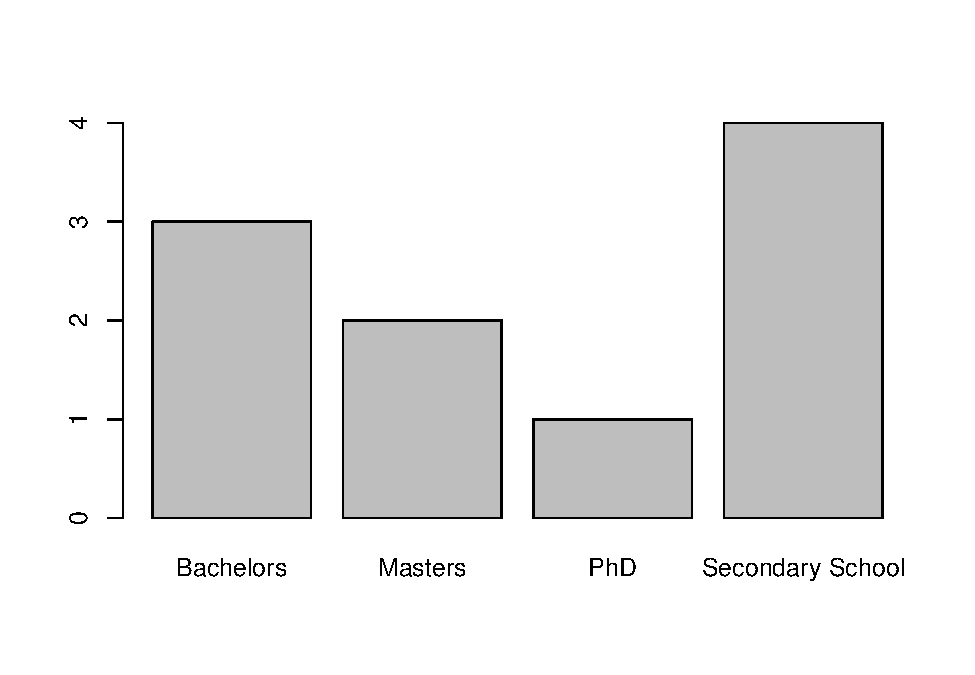
\includegraphics{rintro_demo_files/figure-latex/unnamed-chunk-134-1.pdf}

Now that gives us the information we need, but it's not ordered in an intuitive manner. Ideally, we would want the order of the bar plots to match the hierarchical order of the data, so that it would be: ``Secondary School'', ``Bachelors'', ``Masters'', and then ``PhD''. However, unless you specify the order of your levels, R will specify their order alphabetically.

There is an argument called \texttt{levels} in the \texttt{factor} function that we can use to rectify this. In the levels argument, we specify the order of the levels.

\begin{Shaded}
\begin{Highlighting}[]
\NormalTok{degree\_ordered }\OtherTok{\textless{}{-}} \FunctionTok{factor}\NormalTok{(degree, }\AttributeTok{levels =} \FunctionTok{c}\NormalTok{(}\StringTok{"Secondary School"}\NormalTok{, }\StringTok{"Bachelors"}\NormalTok{, }\StringTok{"Masters"}\NormalTok{, }\StringTok{"PhD"}\NormalTok{))}
\NormalTok{degree\_ordered}
\end{Highlighting}
\end{Shaded}

\begin{verbatim}
##  [1] PhD              Secondary School Masters          Bachelors       
##  [5] Bachelors        Masters          Bachelors        Secondary School
##  [9] Secondary School Secondary School
## Levels: Secondary School Bachelors Masters PhD
\end{verbatim}

That's more like it. Now we can call the \texttt{table()} and \texttt{barplot()} functions again to visualise the number of participants per group.

\begin{Shaded}
\begin{Highlighting}[]
\NormalTok{count\_ordered }\OtherTok{\textless{}{-}} \FunctionTok{table}\NormalTok{(degree\_ordered)}

\FunctionTok{barplot}\NormalTok{(count\_ordered)}
\end{Highlighting}
\end{Shaded}

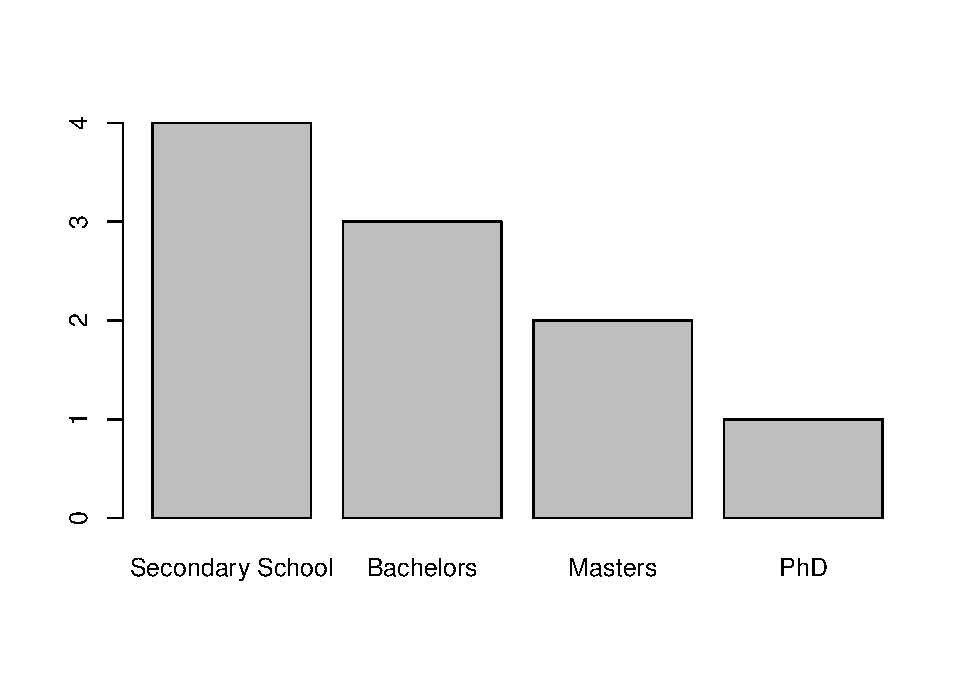
\includegraphics{rintro_demo_files/figure-latex/unnamed-chunk-136-1.pdf}

As you can see, our data looks much cleaner and more intuitive.

There is a lot more we can do with factors, but this covers the main points. Now let's talk about the last data type/structure we are going to be using in this course, which is the \texttt{list} data structure.

\hypertarget{exercises-5}{%
\subsection{Exercises}\label{exercises-5}}

\textbf{Exercise 1 - Convert Numeric Data to Factor:}

\begin{itemize}
\item
  Create a vector called \textbf{\texttt{personality}} containing personality types: ``Introverted'', ``Extroverted'', ``Introverted'', ``Introverted'', ``Extroverted'', ``Extroverted''.
\item
  Convert the \textbf{\texttt{personality}} vector to a factor and store it in a new variable called \textbf{\texttt{personality\_factor}}.
\item
  Display the levels of the \textbf{\texttt{personality\_factor}} variable.
\end{itemize}

\textbf{Exercise 2 - Count and Visualize Factor Levels:}

\begin{itemize}
\item
  Using the created \textbf{\texttt{personality}} vector from Exercise 1, create a table to count the number of occurrences of each Personality trait.
\item
  Visualize the counts using a bar plot to show the distribution of genders.
\end{itemize}

\textbf{Exercise 3 - Modify Factor Levels:}

\begin{Shaded}
\begin{Highlighting}[]
\CommentTok{\# Treatment conditions vector}
\NormalTok{treatment }\OtherTok{\textless{}{-}} \FunctionTok{c}\NormalTok{(}\StringTok{"Control"}\NormalTok{, }\StringTok{"Placebo"}\NormalTok{, }\StringTok{"Therapy"}\NormalTok{, }\StringTok{"Medication"}\NormalTok{, }\StringTok{"Therapy"}\NormalTok{, }\StringTok{"Placebo"}\NormalTok{, }\StringTok{"Control"}\NormalTok{, }\StringTok{"Medication"}\NormalTok{)}
\end{Highlighting}
\end{Shaded}

\begin{itemize}
\item
  Reorder the levels of the \textbf{\texttt{treatment}} vector so that ``Therapy'' becomes the first level, followed by ``Control'', ``Placebo'', and ``Medication''.
\item
  Print the modified levels of the \textbf{\texttt{treatment}} variable to verify the order.
\end{itemize}

\textbf{Exercise 4 - Factor Conversion with Levels:}

\begin{itemize}
\item
  Create a vector called \textbf{\texttt{coping\_strategy}} with the following values: ``Problem-focused'', ``Emotion-focused'', ``Avoidant'', ``Problem-focused'', ``Emotion-focused'', ``Avoidant'', ``Problem-focused''.
\item
  Convert the \textbf{\texttt{coping\_strategy}} vector to a factor with levels specified as ``Problem-focused'', ``Emotion-focused'', ``Avoidant'', and store it in a new variable called \textbf{\texttt{coping\_strategy\_factor}}.
\item
  Display the levels of the \textbf{\texttt{coping\_strategy\_factor}} variable.
\end{itemize}

\hypertarget{the-list-data-structure}{%
\section{The List Data Structure}\label{the-list-data-structure}}

The two data structures we have discussed so far, vectors and data frames, are excellent ways to store data. However, each data structure has its limitations. Both vectors and data frames only allow us to store one object of data at a time.

What do I mean by one object of data? Well, when we create a vector, we are only storing information for one single vector in R. While we can store multiple vectors in one place in R by combining them into a data frame, this is only possible if each vector has the same number of data points. Based on what I have taught you so far, there is no way to store two independent and separate vectors in the same place in R.

Similarly, when I create a data frame, I am only storing information for one data frame. But sometimes we would want to keep multiple data frames saved in a similar location, similar to an Excel file that has multiple worksheets saved onto it.

Finally, what if I wanted to store a vector and a data frame together? For example, imagine I had a data frame that was a cleaned data set, and I wanted to store a vector with results from the analysis. Based on what I have taught you so far, there is no way to store both a vector and a separate data frame in a single space in R.

That's where the list data structure comes into play.

\hypertarget{understanding-lists}{%
\subsection{Understanding Lists}\label{understanding-lists}}

A list in R is a versatile data structure that can hold elements of different types, such as vectors, matrices, data frames, or even other lists. Think of it as a container that can store various objects together, similar to a bag where you can put in items of different shapes and sizes.

\hypertarget{creating-lists}{%
\subsection{Creating Lists}\label{creating-lists}}

Suppose we're conducting a study where we collect various information about each participant, such as their demographic details, test scores, and responses to questionnaires. We can store this information for each participant in a list. Here's how we can create a list for three participants:

\begin{Shaded}
\begin{Highlighting}[]
\NormalTok{participant1 }\OtherTok{\textless{}{-}} \FunctionTok{list}\NormalTok{(}
  \AttributeTok{ID =} \DecValTok{1}\NormalTok{,}
  \AttributeTok{age =} \DecValTok{25}\NormalTok{,}
  \AttributeTok{gender =} \StringTok{"Male"}\NormalTok{,}
  \AttributeTok{test\_scores =} \FunctionTok{c}\NormalTok{(}\DecValTok{80}\NormalTok{, }\DecValTok{75}\NormalTok{, }\DecValTok{90}\NormalTok{),}
  \AttributeTok{questionnaire\_responses =} \FunctionTok{c}\NormalTok{(}\StringTok{"Agree"}\NormalTok{, }\StringTok{"Disagree"}\NormalTok{, }\StringTok{"Neutral"}\NormalTok{, }\StringTok{"Agree"}\NormalTok{)}
\NormalTok{)}

\NormalTok{participant2 }\OtherTok{\textless{}{-}} \FunctionTok{list}\NormalTok{(}
  \AttributeTok{ID =} \DecValTok{2}\NormalTok{,}
  \AttributeTok{age =} \DecValTok{30}\NormalTok{,}
  \AttributeTok{gender =} \StringTok{"Female"}\NormalTok{,}
  \AttributeTok{test\_scores =} \FunctionTok{c}\NormalTok{(}\DecValTok{85}\NormalTok{, }\DecValTok{70}\NormalTok{, }\DecValTok{88}\NormalTok{),}
  \AttributeTok{questionnaire\_responses =} \FunctionTok{c}\NormalTok{(}\StringTok{"Neutral"}\NormalTok{, }\StringTok{"Agree"}\NormalTok{, }\StringTok{"Disagree"}\NormalTok{, }\StringTok{"Strongly Disagree"}\NormalTok{)}
\NormalTok{)}

\NormalTok{participant3 }\OtherTok{\textless{}{-}} \FunctionTok{list}\NormalTok{(}
  \AttributeTok{ID =} \DecValTok{3}\NormalTok{,}
  \AttributeTok{age =} \DecValTok{28}\NormalTok{,}
  \AttributeTok{gender =} \StringTok{"Non{-}binary"}\NormalTok{,}
  \AttributeTok{test\_scores =} \FunctionTok{c}\NormalTok{(}\DecValTok{78}\NormalTok{, }\DecValTok{82}\NormalTok{, }\DecValTok{85}\NormalTok{),}
  \AttributeTok{questionnaire\_responses =} \FunctionTok{c}\NormalTok{(}\StringTok{"Disagree"}\NormalTok{, }\StringTok{"Neutral"}\NormalTok{, }\StringTok{"Agree"}\NormalTok{, }\StringTok{"Neutral"}\NormalTok{)}
\NormalTok{)}
\end{Highlighting}
\end{Shaded}

The list for each participant is made up of separate vectors with varying lengths (e.g., there is only 1 element in ID, age, and gender, whereas there are 3 elements in test\_scores and 4 in questionnaire\_responses).

Let's print out the \textbf{\texttt{participant1}} list and break down the output:

\begin{Shaded}
\begin{Highlighting}[]
\FunctionTok{print}\NormalTok{(participant1)}
\end{Highlighting}
\end{Shaded}

\begin{verbatim}
## $ID
## [1] 1
## 
## $age
## [1] 25
## 
## $gender
## [1] "Male"
## 
## $test_scores
## [1] 80 75 90
## 
## $questionnaire_responses
## [1] "Agree"    "Disagree" "Neutral"  "Agree"
\end{verbatim}

When we print out the list, what R does in the console is print out the name of each object and then print out each element in that object. One thing that you might notice is the return of the \texttt{\$} which we use to access elements from vectors or columns from data frames. Luckily, we can also use the \texttt{\$} symbol to access objects and their elements from a list. So I wanted to extract \texttt{test\_scores} from a list, I could type the following code:

\begin{Shaded}
\begin{Highlighting}[]
\NormalTok{participant1}\SpecialCharTok{$}\NormalTok{test\_scores}
\end{Highlighting}
\end{Shaded}

\begin{verbatim}
## [1] 80 75 90
\end{verbatim}

I could also do this numerically using the {[}{]} notation we used when accessing vectors.

\begin{Shaded}
\begin{Highlighting}[]
\NormalTok{participant1[}\DecValTok{4}\NormalTok{]}
\end{Highlighting}
\end{Shaded}

\begin{verbatim}
## $test_scores
## [1] 80 75 90
\end{verbatim}

Because \texttt{test\_scores} is the fourth object within the list (the first three are ID, age, and gender), \texttt{test\_scores{[}4{]}} is needed to extract it.

Regardless of which way you extract data, doesn't the output should look familiar? It is essential the same output when we print out a vector. That's not accidental, because we have in fact extracted a vector!

So what could we do if wanted to access the 1st and 3rd element from this vector? We just follow the same convention that we used last week \texttt{vectorname{[}elementswewant{]}}

\begin{Shaded}
\begin{Highlighting}[]
\NormalTok{participant1}\SpecialCharTok{$}\NormalTok{test\_scores[}\FunctionTok{c}\NormalTok{(}\DecValTok{1}\NormalTok{, }\DecValTok{3}\NormalTok{)]}
\end{Highlighting}
\end{Shaded}

\begin{verbatim}
## [1] 80 90
\end{verbatim}

This illustrates a key point about lists. Once you first access an object (e.g., vector or dataframe) within that list, then you can use the specific indexing criteria for accessing elements within that object. For example, let's look at a list with a vector and a data frame.

\begin{Shaded}
\begin{Highlighting}[]
\NormalTok{df\_v }\OtherTok{\textless{}{-}} \FunctionTok{list}\NormalTok{(}
  \AttributeTok{iq\_df =}\NormalTok{ iq\_df, }
  \AttributeTok{p\_values =} \FunctionTok{c}\NormalTok{(.}\DecValTok{001}\NormalTok{, .}\DecValTok{10}\NormalTok{, .}\DecValTok{05}\NormalTok{)}
\NormalTok{)}

\FunctionTok{print}\NormalTok{(df\_v)}
\end{Highlighting}
\end{Shaded}

\begin{verbatim}
## $iq_df
##   ID age  iq iq_z_scores total_depression_beck
## 1  1  22 100   0.0000000                    32
## 2  2  30 123   1.5333333                    36
## 3  3  41 111   0.7333333                    34
## 4  4  45 130   2.0000000                    46
## 5  5  18  90  -0.6666667                    30
## 6  6  21 102   0.1333333                    53
## 7  7  23  88  -0.8000000                    40
## 8  8  45 109   0.6000000                    15
## 
## $p_values
## [1] 0.001 0.100 0.050
\end{verbatim}

We can see that the first object in our list is the iq\_df data frame, and the second contains (totally made up) p-values. So if wanted to access the \texttt{iq} and \texttt{total\_depression\_beck} columns from this data frame, and the first five rows, we can use the same subsetting techniques we learned last week: \texttt{dataframe{[}rows\_we\_want,\ columns\_we\_want{]}}

\begin{Shaded}
\begin{Highlighting}[]
\NormalTok{df\_v}\SpecialCharTok{$}\NormalTok{iq\_df[}\DecValTok{1}\SpecialCharTok{:}\DecValTok{5}\NormalTok{, }\FunctionTok{c}\NormalTok{(}\StringTok{"iq"}\NormalTok{, }\StringTok{"total\_depression\_beck"}\NormalTok{)]}
\end{Highlighting}
\end{Shaded}

\begin{verbatim}
##    iq total_depression_beck
## 1 100                    32
## 2 123                    36
## 3 111                    34
## 4 130                    46
## 5  90                    30
\end{verbatim}

\hypertarget{lists-within-lists-indexing}{%
\subsection{Lists within Lists (Indexing)}\label{lists-within-lists-indexing}}

What happens if we combine lists together? Well, we can do that by putting lists inside lists. However, if we do that, the output might seem a bit overwhelming at first.

\begin{Shaded}
\begin{Highlighting}[]
\NormalTok{participant\_data }\OtherTok{\textless{}{-}} \FunctionTok{list}\NormalTok{(participant1, participant2, participant3)}
 
\FunctionTok{print}\NormalTok{(participant\_data)}
\end{Highlighting}
\end{Shaded}

\begin{verbatim}
## [[1]]
## [[1]]$ID
## [1] 1
## 
## [[1]]$age
## [1] 25
## 
## [[1]]$gender
## [1] "Male"
## 
## [[1]]$test_scores
## [1] 80 75 90
## 
## [[1]]$questionnaire_responses
## [1] "Agree"    "Disagree" "Neutral"  "Agree"   
## 
## 
## [[2]]
## [[2]]$ID
## [1] 2
## 
## [[2]]$age
## [1] 30
## 
## [[2]]$gender
## [1] "Female"
## 
## [[2]]$test_scores
## [1] 85 70 88
## 
## [[2]]$questionnaire_responses
## [1] "Neutral"           "Agree"             "Disagree"         
## [4] "Strongly Disagree"
## 
## 
## [[3]]
## [[3]]$ID
## [1] 3
## 
## [[3]]$age
## [1] 28
## 
## [[3]]$gender
## [1] "Non-binary"
## 
## [[3]]$test_scores
## [1] 78 82 85
## 
## [[3]]$questionnaire_responses
## [1] "Disagree" "Neutral"  "Agree"    "Neutral"
\end{verbatim}

Right now your eyes might be glazing over and that SPSS icon on your desktop has never looked so good. But just relax, while what you might be seeing here is \textbf{ugly}, I promise you it's not complicated.

Let's break down the first part of this output

\begin{Shaded}
\begin{Highlighting}[]
\NormalTok{[[}\DecValTok{1}\NormalTok{]]}
\end{Highlighting}
\end{Shaded}

This notation \textbf{\texttt{{[}{[}1{]}{]}}} extracts and indicates the first list within our combined list \textbf{\texttt{participant\_data}} (in this case participant1). Similarly, \textbf{\texttt{{[}{[}2{]}{]}}} would indicate the second list (participant2), and so on. It's similar to how we index elements in vectors.

\begin{Shaded}
\begin{Highlighting}[]
\NormalTok{[[}\DecValTok{1}\NormalTok{]]}\SpecialCharTok{$}\NormalTok{ID }\CommentTok{\#this translates to from participant data, pick participant 1 and then extract ID}

\NormalTok{[[}\DecValTok{1}\NormalTok{]]}\SpecialCharTok{$}\NormalTok{age }\CommentTok{\#this translates to from participant data, pick participant 1 and then extract age}

\NormalTok{[[}\DecValTok{1}\NormalTok{]]}\SpecialCharTok{$}\NormalTok{test\_scores }\CommentTok{\#this translates to from participant data, pick participant 1 and then extract test scores}

\NormalTok{[[}\DecValTok{1}\NormalTok{]]}\SpecialCharTok{$}\NormalTok{questionnaire\_responses }\CommentTok{\#this translates to from participant data, pick participant 1 and then questionnaire\_responses}
\end{Highlighting}
\end{Shaded}

Basically translates to ``participant 1's data for ID, age, test\_scores and questionnaire\_responses''.

There is a way we can make this code output neater. When we are creating a list, we can specify the index term for that list. The syntax for doing is: new index term = current\_list

\begin{Shaded}
\begin{Highlighting}[]
\NormalTok{participant\_data }\OtherTok{\textless{}{-}} \FunctionTok{list}\NormalTok{(}\AttributeTok{p1 =}\NormalTok{ participant1, }\CommentTok{\#new index term = current list}
                         \AttributeTok{p2 =}\NormalTok{ participant2, }\CommentTok{\#new index term = current list}
                         \AttributeTok{p3 =}\NormalTok{ participant3 }\CommentTok{\#new index term = current list}
\NormalTok{                         )}

\FunctionTok{print}\NormalTok{(participant\_data)}
\end{Highlighting}
\end{Shaded}

\begin{verbatim}
## $p1
## $p1$ID
## [1] 1
## 
## $p1$age
## [1] 25
## 
## $p1$gender
## [1] "Male"
## 
## $p1$test_scores
## [1] 80 75 90
## 
## $p1$questionnaire_responses
## [1] "Agree"    "Disagree" "Neutral"  "Agree"   
## 
## 
## $p2
## $p2$ID
## [1] 2
## 
## $p2$age
## [1] 30
## 
## $p2$gender
## [1] "Female"
## 
## $p2$test_scores
## [1] 85 70 88
## 
## $p2$questionnaire_responses
## [1] "Neutral"           "Agree"             "Disagree"         
## [4] "Strongly Disagree"
## 
## 
## $p3
## $p3$ID
## [1] 3
## 
## $p3$age
## [1] 28
## 
## $p3$gender
## [1] "Non-binary"
## 
## $p3$test_scores
## [1] 78 82 85
## 
## $p3$questionnaire_responses
## [1] "Disagree" "Neutral"  "Agree"    "Neutral"
\end{verbatim}

\hypertarget{summary-2}{%
\subsection{Summary}\label{summary-2}}

In summary, the list data structure in R is incredibly useful for organizing and managing diverse types of data in psychological research. Whether it's participant information, experimental conditions, or any other heterogeneous data, lists provide a flexible and efficient way to store and access this information.

\hypertarget{r-packages}{%
\section{R Packages}\label{r-packages}}

Throughout this course, we've been exploring the capabilities of base R, which offers a rich set of functions and data structures for data analysis and statistical computing. However, the power of R extends far beyond its base functionality, thanks to its vibrant ecosystem of user-contributed packages.

\hypertarget{understanding-r-packages}{%
\subsection{Understanding R Packages}\label{understanding-r-packages}}

R packages are collections of R functions, data, and documentation that extend the capabilities of R. These packages are developed and shared by the R community to address various needs in data analysis, visualization, machine learning, and more. By leveraging packages, R users can access a vast array of specialized tools and algorithms without reinventing the wheel.

\hypertarget{installing-and-loading-r-package}{%
\subsection{Installing and Loading R Package}\label{installing-and-loading-r-package}}

One of the most important things to know about R packages is that you first need to install them on your computer. Once installed, you will not need to install them again.

However, if you want to use a package, then you will need to load it while you are in RStudio. Every time you open RStudio after closing it, you will need to load that package again if you want to use it.

In this way, R packages are like applications on your phone. Once you download Spotify on your phone, then you won't need to install it again. But every time you want to use Spotify, you will need to open the application.

\hypertarget{installation}{%
\subsubsection{Installation}\label{installation}}

We are going to install three packages called Haven, praise, and fortunes. The praise package provides users with, well, praise. And the fortunes package will spit out statistic and programming quotes at you. Neither of them is particularly useful, other than demonstrating the process of loading packages.

The Haven package enables you to load SPSS data into R.

\hypertarget{installation-using-rstudio-interface}{%
\subsubsection{Installation using RStudio Interface}\label{installation-using-rstudio-interface}}

In the Files pane on the bottom right-hand corner of R, you will see a tab called ``Packages''. Click that tab. You will already see a list of packages that are currently installed. You will see three columns:

\begin{itemize}
\item
  Name (the name of the R package)
\item
  Description (describes what the package does)
\item
  Version (the version of the package currently installed on your computer)
\end{itemize}

To install a package, click the ``Install'' button above the ``Name'' column. Once you click that, you should see a small pop-up window. In the textbox, type in the word Haven. Make sure the box ``Install dependencies'' is clicked. After that, you can click Install. You should get something like the following output in the console, which looks scary with all the red text, but means it has worked correctly.

\begin{Shaded}
\begin{Highlighting}[]
\SpecialCharTok{\textgreater{}} \FunctionTok{install.packages}\NormalTok{(}\StringTok{"Haven"}\NormalTok{)}
\NormalTok{trying URL }\StringTok{\textquotesingle{}https://cran.rstudio.com/bin/macosx/big{-}sur{-}x86\_64/contrib/4.3/rio\_1.0.1.tgz\textquotesingle{}}
\NormalTok{Content type }\StringTok{\textquotesingle{}application/x{-}gzip\textquotesingle{}}\NormalTok{ length }\DecValTok{591359} \FunctionTok{bytes}\NormalTok{ (}\DecValTok{577}\NormalTok{ KB)}
\SpecialCharTok{==}\ErrorTok{================================================}
\NormalTok{downloaded }\DecValTok{577}\NormalTok{ KB}


\NormalTok{The downloaded binary packages are }\ControlFlowTok{in}
    \SpecialCharTok{/}\NormalTok{var}\SpecialCharTok{/}\NormalTok{folders}\SpecialCharTok{/}\NormalTok{h8}\SpecialCharTok{/}\NormalTok{8sb24v\_x2lg51cg2z7q8fk3w0000gp}\SpecialCharTok{/}\NormalTok{T}\SpecialCharTok{/}\ErrorTok{/}\NormalTok{RtmpvaY1Ue}\SpecialCharTok{/}\NormalTok{downloaded\_packages}
\end{Highlighting}
\end{Shaded}

\hypertarget{installation-using-commands}{%
\subsubsection{Installation using Commands}\label{installation-using-commands}}

If we want to install packages using the console, you can use the \textbf{\texttt{install.packages()}} function followed by the name of the package you wish to install. The syntax would looks like this

\begin{Shaded}
\begin{Highlighting}[]
\FunctionTok{install.packages}\NormalTok{(}\StringTok{"package name"}\NormalTok{)}
\end{Highlighting}
\end{Shaded}

The important thing here is that whatever goes inside the parentheses is inside quotation marks. Let's use this syntax to install the \texttt{praise} and \texttt{fortunes} packages.

\begin{Shaded}
\begin{Highlighting}[]
\FunctionTok{install.packages}\NormalTok{(}\FunctionTok{c}\NormalTok{(}\StringTok{"praise"}\NormalTok{, }\StringTok{"fortunes"}\NormalTok{))}


\NormalTok{trying URL }\StringTok{\textquotesingle{}https://cran.rstudio.com/bin/macosx/big{-}sur{-}x86\_64/contrib/4.3/praise\_1.0.0.tgz\textquotesingle{}}
\NormalTok{Content type }\StringTok{\textquotesingle{}application/x{-}gzip\textquotesingle{}}\NormalTok{ length }\DecValTok{16537} \FunctionTok{bytes}\NormalTok{ (}\DecValTok{16}\NormalTok{ KB)}
\SpecialCharTok{==}\ErrorTok{================================================}
\NormalTok{downloaded }\DecValTok{16}\NormalTok{ KB}

\NormalTok{trying URL }\StringTok{\textquotesingle{}https://cran.rstudio.com/bin/macosx/big{-}sur{-}x86\_64/contrib/4.3/fortunes\_1.5{-}4.tgz\textquotesingle{}}
\NormalTok{Content type }\StringTok{\textquotesingle{}application/x{-}gzip\textquotesingle{}}\NormalTok{ length }\DecValTok{208808} \FunctionTok{bytes}\NormalTok{ (}\DecValTok{203}\NormalTok{ KB)}
\SpecialCharTok{==}\ErrorTok{================================================}
\NormalTok{downloaded }\DecValTok{203}\NormalTok{ KB}


\NormalTok{The downloaded binary packages are }\ControlFlowTok{in}
    \SpecialCharTok{/}\NormalTok{var}\SpecialCharTok{/}\NormalTok{folders}\SpecialCharTok{/}\NormalTok{h8}\SpecialCharTok{/}\NormalTok{8sb24v\_x2lg51cg2z7q8fk3w0000gp}\SpecialCharTok{/}\NormalTok{T}\SpecialCharTok{/}\ErrorTok{/}\NormalTok{RtmpvaY1Ue}\SpecialCharTok{/}\NormalTok{downloaded\_packages}
\end{Highlighting}
\end{Shaded}

Again the output is rather scary but the sentences ``package `praise' successfully unpacked and MD5 sums checked'' and ``package `fortunes' successfully unpacked and MD5 sums checked'' mean that they are successfully installed onto your computer.

\hypertarget{loading-packages}{%
\subsection{Loading Packages}\label{loading-packages}}

Okay, now to actually use those packages, we will need to load them. Again, I will show you two ways to load packages.

\hypertarget{loading-using-rstudio-interface}{%
\subsubsection{Loading using RStudio Interface}\label{loading-using-rstudio-interface}}

Go back to the Packages tab in the File pane. On the left-hand side of the package name, you will see a tick box. If the box is ticked, that means the package is currently loaded. If it is unticked, it is not loaded.

Scroll down to find the package ``praise'' and load it by ticking the box.

\begin{figure}
\centering
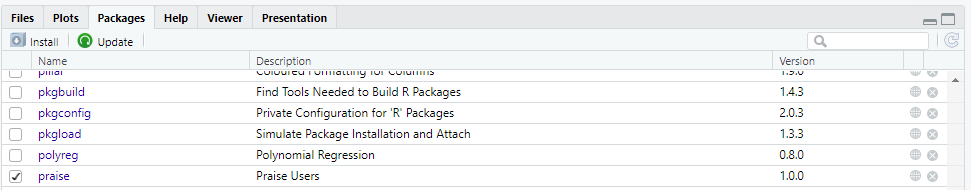
\includegraphics{img/04-praise-loaded.png}
\caption{\label{fig:unnamed-chunk-152}Loading Packages through RStudio Interface}
\end{figure}

You should see something like the following in your R console (don't worry if you get a warning message like mine, or if you don't receive a warning message)

\begin{Shaded}
\begin{Highlighting}[]
\SpecialCharTok{\textgreater{}} \FunctionTok{library}\NormalTok{(praise)}
\NormalTok{Warning message}\SpecialCharTok{:}
\NormalTok{package ‘praise’ was built under R version }\DecValTok{4}\NormalTok{.}\FloatTok{3.2} 
\end{Highlighting}
\end{Shaded}

\hypertarget{loading-using-the-r-console-command}{%
\subsubsection{Loading using the R Console Command}\label{loading-using-the-r-console-command}}

We can use the same syntax from that R console output to load in packages there. To load in the \texttt{fortunes} and \texttt{Haven} packages, you can type in the following into the console or script one at a time:

\begin{Shaded}
\begin{Highlighting}[]
\FunctionTok{library}\NormalTok{(fortunes)}
\FunctionTok{library}\NormalTok{(haven)}
\end{Highlighting}
\end{Shaded}

\begin{verbatim}
## Warning: package 'haven' was built under R version 4.3.2
\end{verbatim}

There is one significant difference between installing and loading packages through code. When you are installing packages, you can install multiple packages in one command. However, you can only load one package at a time

\begin{Shaded}
\begin{Highlighting}[]
\CommentTok{\#will work}
\FunctionTok{install.packages}\NormalTok{(}\FunctionTok{c}\NormalTok{(}\StringTok{"package1"}\NormalTok{, }\StringTok{"package2"}\NormalTok{, }\StringTok{"package3"}\NormalTok{)) }


\CommentTok{\#will not work}
\FunctionTok{library}\NormalTok{(}\FunctionTok{c}\NormalTok{(}\StringTok{"package1"}\NormalTok{, }\StringTok{"package2"}\NormalTok{, }\StringTok{"package3"}\NormalTok{)) }

\CommentTok{\#the following will work}
\FunctionTok{library}\NormalTok{(package1)}
\FunctionTok{library}\NormalTok{(package2)}
\FunctionTok{library}\NormalTok{(package3)}
\end{Highlighting}
\end{Shaded}

\hypertarget{testing-our-new-functions}{%
\subsection{Testing our New Functions}\label{testing-our-new-functions}}

To make sure the following functions are working, run the following code to check:

\begin{verbatim}
## Warning: package 'praise' was built under R version 4.3.2
\end{verbatim}

\begin{verbatim}
## [1] "You are priceless!"
\end{verbatim}

\begin{verbatim}
## 
## Soham: How to compute the p-value of a statistic generally?
## Berton Gunter: runif(1)
##    -- Soham and Berton Gunter
##       R-help (May 2010)
\end{verbatim}

\begin{Shaded}
\begin{Highlighting}[]
\FunctionTok{praise}\NormalTok{() }\CommentTok{\#everytime you run this line of code it gives you a different line of praise}
\CommentTok{\#so don\textquotesingle{}t be worried if your result is different than mine}

\FunctionTok{fortune}\NormalTok{() }\CommentTok{\#this will print out something so incredibly nerdy }
\end{Highlighting}
\end{Shaded}

\hypertarget{error-loading-packages}{%
\subsection{Error Loading Packages}\label{error-loading-packages}}

If you ever encounter the following error when trying to load a package:

\begin{Shaded}
\begin{Highlighting}[]
\FunctionTok{library}\NormalTok{(madeuppackage)}
\end{Highlighting}
\end{Shaded}

\begin{verbatim}
## Error in library(madeuppackage): there is no package called 'madeuppackage'
\end{verbatim}

This means that you have either made a typo in writing the name of the package or you have not installed the package. You need to install packages before R will be able to load them.

\hypertarget{package-conventions-if-using-code}{%
\subsection{Package Conventions if Using Code}\label{package-conventions-if-using-code}}

There are important rules to follow when writing code to install and load packages in R.

Firstly, any packages you install and load onto R should be placed at the top of the R script you are working on. This way, anyone following your analysis can easily spot the packages they will need.

Secondly, you should type the command \textbf{\texttt{install.packages("package\_name")}} in the console rather than the script. If someone downloads your script and accidentally runs it, it will automatically install the packages on their computer. We want to avoid this as it might interfere with other aspects of their operating system (this is rare, but it's better to be cautious).

Thirdly, if you do include the command \textbf{\texttt{install.packages()}} in the script, make sure it is commented out. This way, if it is accidentally run, R won't execute that command.

\begin{figure}
\centering
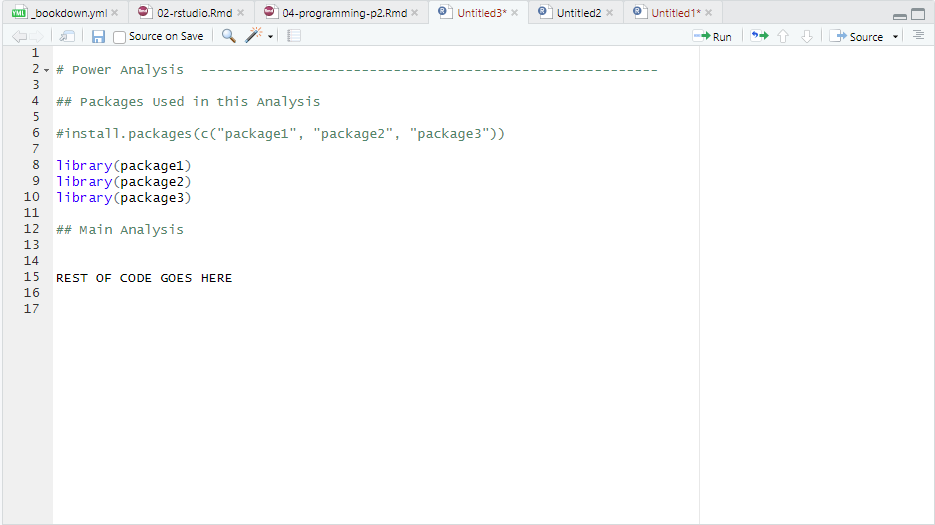
\includegraphics{img/04-packages-convention.png}
\caption{\label{fig:unnamed-chunk-159}Conventions for Installing and Loading Packages in R Script}
\end{figure}

\hypertarget{summary-3}{%
\subsection{Summary}\label{summary-3}}

There you have it. You have successfully installed and loaded your first packages in R. Are they particularly useful packages? No! In the rest of this course, we will be loading packages more regularly, and these packages will make our lives significantly easier than if they were not around. In fact, we will use the \texttt{haven} package in the next section that will enable us to import SPSS data.

\hypertarget{importing}{%
\section{Importing and Exporting Data}\label{importing}}

While creating data frames and lists in R is valuable, the majority of the data you'll work with in R will likely come from external sources. Therefore, it's essential to know how to import data into R. Similarly, once you've processed and analyzed your data in R, you'll often need to export it for further use or sharing.

In this section, we'll explore how to import and export data using the graphical user interface (GUI) provided by RStudio. The GUI offers a user-friendly and intuitive way to manage data files without requiring you to write any code. Let's delve into the process of importing and exporting data using the RStudio GUI.

First, you'll need to download two files: \texttt{psycho.csv} and \texttt{burnout.sav}. Both files are available in the rintro Teams channel. If you don't have access to the Teams channel, please contact me at ryan.donovan@universityofgalway.ie.

\hypertarget{importing-csv-files.}{%
\subsection{Importing CSV files.}\label{importing-csv-files.}}

Comma-Separated Values (CSV) files are a prevalent format for storing tabular data. Similar to Excel files, data in CSV files is organized into rows and columns, with each row representing a single record and each column representing a different attribute or variable.

CSV files are plain text files, making them easy to create, edit, and view using a simple text editor. This simplicity and universality make CSV files a popular choice for data exchange across various applications and platforms.

In a CSV file, each value in the table is separated by a comma (,), hence the name ``comma-separated values.'' However, depending on locale settings, other delimiters such as semicolons (;) or tabs (\textbackslash t) may be used instead.

One of the key advantages of CSV files is their compatibility with a wide range of software and programming languages, including R. They can be effortlessly imported into statistical software for analysis, making them a versatile and widely adopted format for data storage and sharing.

To import the ``psycho.csv'' file, please follow these steps:

\begin{enumerate}
\def\labelenumi{\arabic{enumi}.}
\item
  Open RStudio.
\item
  Navigate to the Environment pane (top right hand corner) and make sure the Environment tab is clicked.
\item
  Click on the ``Import Dataset'' button.
\item
  Select ``From Text (base)''.
\item
  Browse your folder and select the ``psycho.csv'' to import.
\item
  Click ``Open''.
\item
  A pop-up window should now open. There is a lot of different information here, so let's unpack it.

  \begin{itemize}
  \item
    The ``Name'' text box enables you to specify the variable name assigned to the data frame. Leave it as ``psycho.''
  \item
    Most of the time, you can leave the options with the default settings.
  \item
    The ``Input File'' box shows a preview of the CSV file being imported.
  \item
    The ``Data Frame'' box displays a preview of how the data frame will look once the CSV is imported into R.
  \end{itemize}
\end{enumerate}

\begin{Shaded}
\begin{Highlighting}[]
\FunctionTok{library}\NormalTok{(knitr)}

\FunctionTok{include\_graphics}\NormalTok{(}\StringTok{"img/04{-}import{-}csv.png"}\NormalTok{)}
\end{Highlighting}
\end{Shaded}

\begin{figure}
\centering
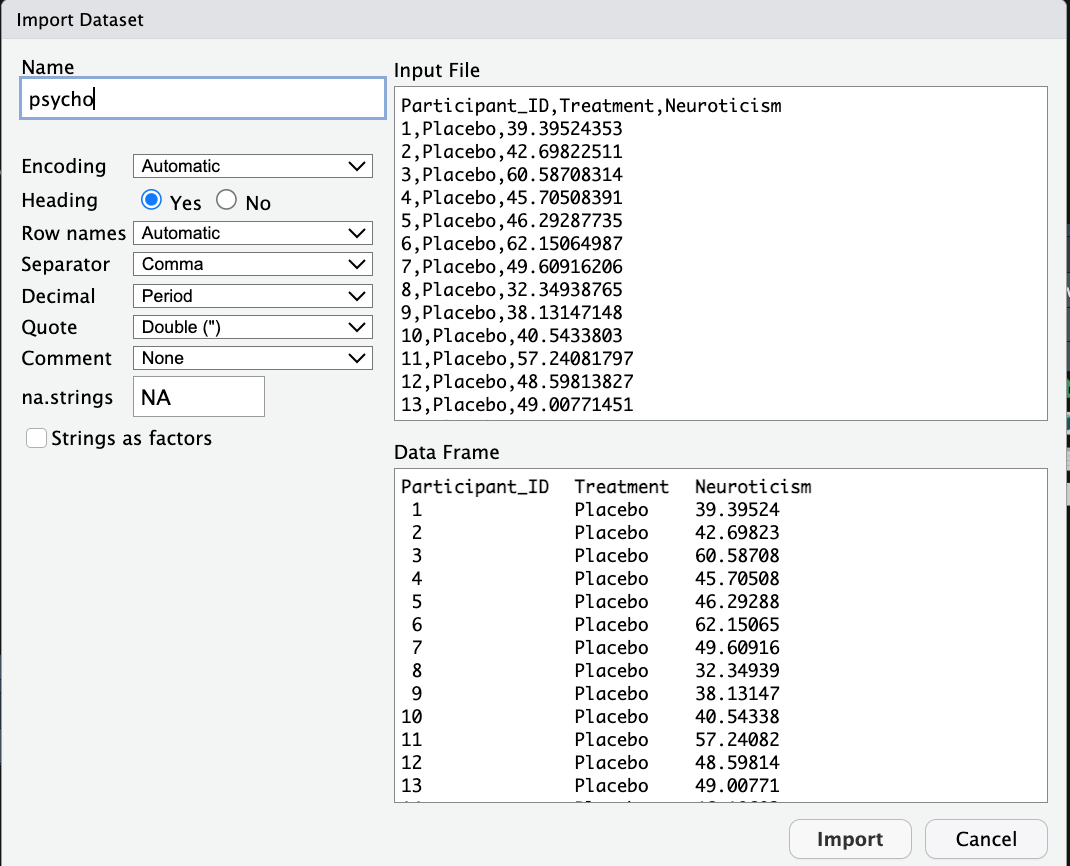
\includegraphics{img/04-import-csv.png}
\caption{\label{fig:unnamed-chunk-160}Pop-up window for importing CSV files}
\end{figure}

\begin{enumerate}
\def\labelenumi{\arabic{enumi}.}
\setcounter{enumi}{7}
\tightlist
\item
  Click Import. A tab in the source pane called ``psycho'' should now open showing the data frame. Additionally, you should also see the data frame in the Environment pane. You should see under value that it has ``60 obs. of 3 variables'' which means there are 60 rows of data and 3 columns of data.
\item
  Once you have imported your data in R, it is always good practice to briefly check that it has been imported successfully and you have imported the correct data set. Two ways you can do this is by calling the \texttt{head()} and \texttt{summary()} functions on the data frame.
\end{enumerate}

\begin{Shaded}
\begin{Highlighting}[]
\FunctionTok{head}\NormalTok{(psycho) }\CommentTok{\#this will print out the first six rows}
\end{Highlighting}
\end{Shaded}

\begin{verbatim}
##   Participant_ID Treatment Neuroticism
## 1              1   Placebo    39.39524
## 2              2   Placebo    42.69823
## 3              3   Placebo    60.58708
## 4              4   Placebo    45.70508
## 5              5   Placebo    46.29288
## 6              6   Placebo    62.15065
\end{verbatim}

\begin{Shaded}
\begin{Highlighting}[]
\FunctionTok{summary}\NormalTok{(psycho) }\CommentTok{\#print out summary stats for each column}
\end{Highlighting}
\end{Shaded}

\begin{verbatim}
##  Participant_ID   Treatment          Neuroticism   
##  Min.   : 1.00   Length:60          Min.   :25.33  
##  1st Qu.:15.75   Class :character   1st Qu.:41.75  
##  Median :30.50   Mode  :character   Median :49.44  
##  Mean   :30.50                      Mean   :48.99  
##  3rd Qu.:45.25                      3rd Qu.:54.61  
##  Max.   :60.00                      Max.   :76.69
\end{verbatim}

If your results match mine, it means you have correctly imported the data.

\hypertarget{importing-spss-.sav-files.}{%
\subsection{Importing SPSS (.sav files).}\label{importing-spss-.sav-files.}}

SPSS (Statistical Package for the Social Sciences) is another popular software used for statistical analysis, particularly in the social sciences. SPSS data files are typically saved with a \textbf{\texttt{.sav}} extension. These files can contain data, variable names, variable labels, and other metadata.

To import an SPSS file (\textbf{\texttt{burnout.sav}}), follow these steps:

\begin{enumerate}
\def\labelenumi{\arabic{enumi}.}
\item
  Open RStudio.
\item
  Navigate to the Environment pane (top right-hand corner) and make sure the Environment tab is clicked.
\item
  Click on the ``Import Dataset'' button.
\item
  Select ``From SPSS''.
\item
  A pop-up window will open.
\end{enumerate}

\begin{Shaded}
\begin{Highlighting}[]
\FunctionTok{include\_graphics}\NormalTok{(}\StringTok{"img/04{-}import{-}sav.png"}\NormalTok{)}
\end{Highlighting}
\end{Shaded}

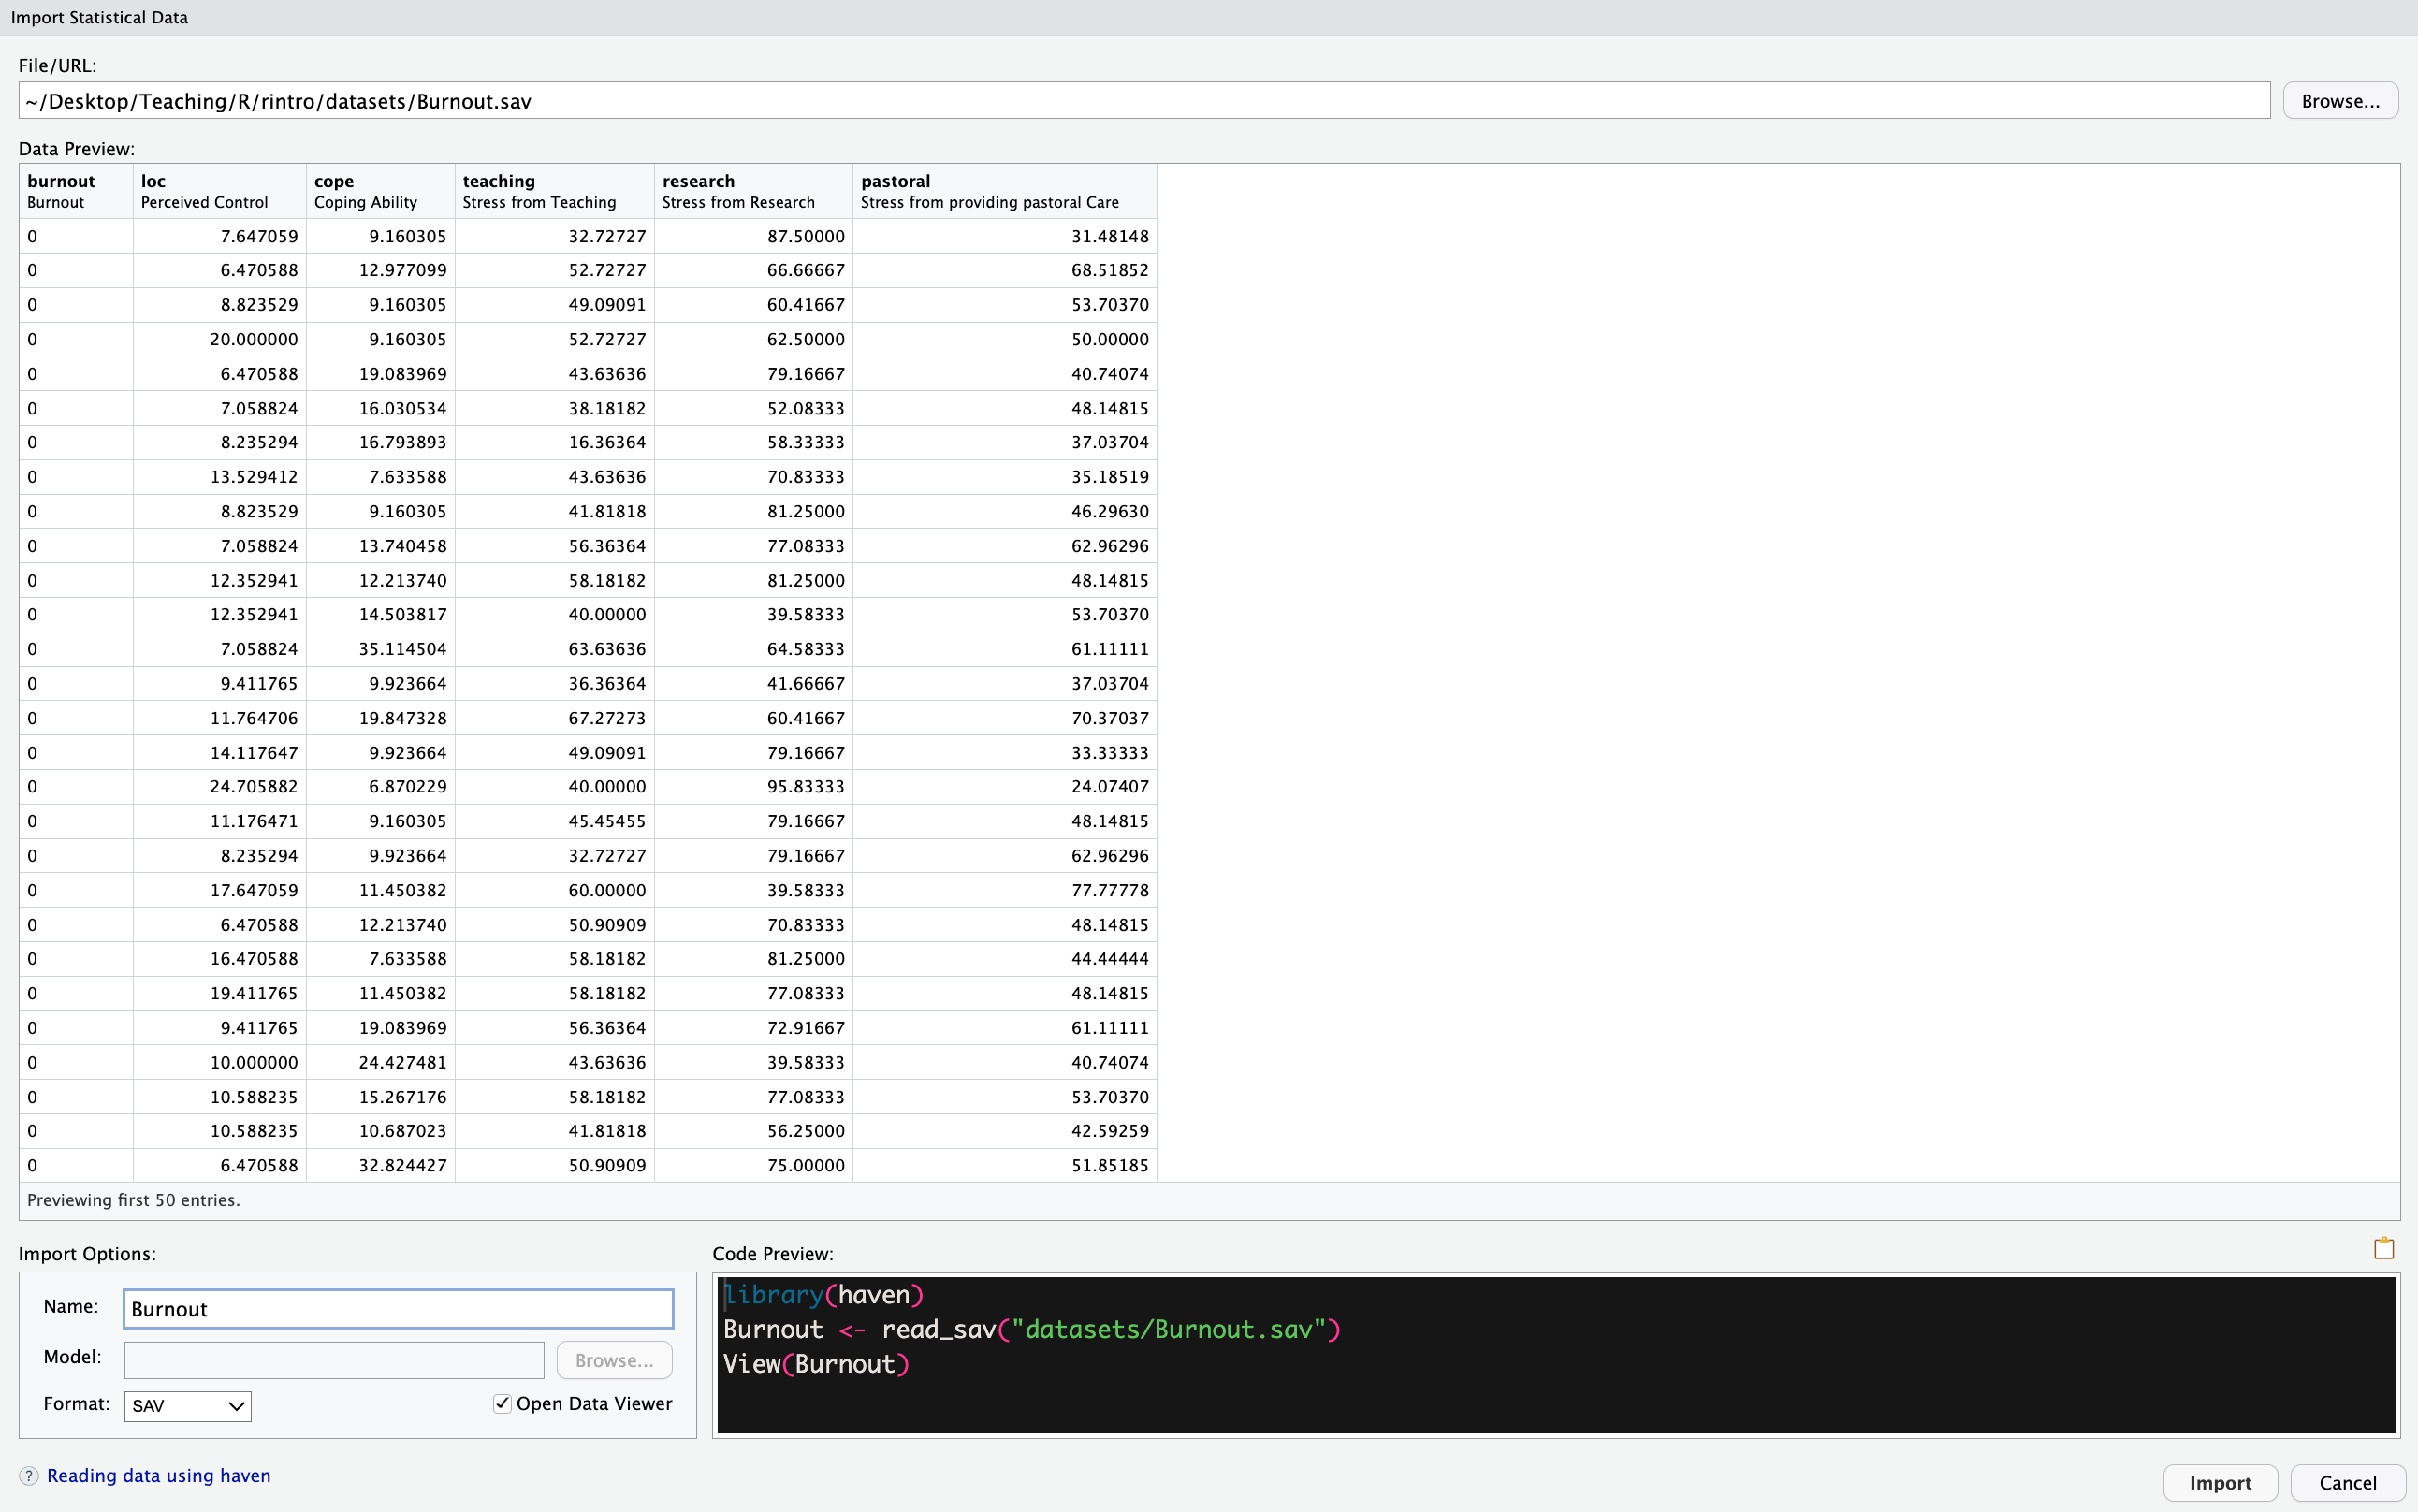
\includegraphics{img/04-import-sav.png}

\begin{enumerate}
\def\labelenumi{\arabic{enumi}.}
\setcounter{enumi}{5}
\item
  Browse your folder and select the \textbf{\texttt{burnout.sav}} file to import.
\item
  Under Import Options, you can set the name of the data frame variable in R for the SPSS data set. Leave it as \texttt{burnout.sav}.
\item
  The Code Preview shows you the written code commands that you could type out to import the data frame instead of using the RStudio interface.
\item
  To import the dataframe, click ``Import''.
\end{enumerate}

After importing, a tab in the source pane called ``burnout'' should open, displaying the data frame. Additionally, you should see the data frame in the Environment pane. Under the ``value'' column, it should indicate ``467 obs. of 6 variables,'' indicating there are 467 rows and 6 columns of data.

Once imported, use the \textbf{\texttt{head()}} and \textbf{\texttt{summary()}} functions to check that the data has been imported correctly:

\begin{Shaded}
\begin{Highlighting}[]
\FunctionTok{head}\NormalTok{(Burnout)}
\end{Highlighting}
\end{Shaded}

\begin{verbatim}
## # A tibble: 6 x 6
##   burnout             loc  cope teaching research pastoral
##   <dbl+lbl>         <dbl> <dbl>    <dbl>    <dbl>    <dbl>
## 1 0 [Not Burnt Out]  7.65  9.16     32.7     87.5     31.5
## 2 0 [Not Burnt Out]  6.47 13.0      52.7     66.7     68.5
## 3 0 [Not Burnt Out]  8.82  9.16     49.1     60.4     53.7
## 4 0 [Not Burnt Out] 20     9.16     52.7     62.5     50  
## 5 0 [Not Burnt Out]  6.47 19.1      43.6     79.2     40.7
## 6 0 [Not Burnt Out]  7.06 16.0      38.2     52.1     48.1
\end{verbatim}

\begin{Shaded}
\begin{Highlighting}[]
\FunctionTok{summary}\NormalTok{(Burnout)}
\end{Highlighting}
\end{Shaded}

\begin{verbatim}
##     burnout            loc               cope            teaching     
##  Min.   :0.0000   Min.   :  6.471   Min.   :  3.817   Min.   : 16.36  
##  1st Qu.:0.0000   1st Qu.:  9.412   1st Qu.: 12.214   1st Qu.: 47.27  
##  Median :0.0000   Median : 14.118   Median : 19.084   Median : 54.55  
##  Mean   :0.2548   Mean   : 17.900   Mean   : 23.919   Mean   : 55.43  
##  3rd Qu.:1.0000   3rd Qu.: 22.353   3rd Qu.: 31.298   3rd Qu.: 61.82  
##  Max.   :1.0000   Max.   :100.000   Max.   :100.000   Max.   :100.00  
##     research         pastoral     
##  Min.   : 20.83   Min.   : 18.52  
##  1st Qu.: 52.08   1st Qu.: 46.30  
##  Median : 62.50   Median : 53.70  
##  Mean   : 61.91   Mean   : 55.25  
##  3rd Qu.: 72.92   3rd Qu.: 62.96  
##  Max.   :100.00   Max.   :100.00
\end{verbatim}

If your results match mine, then you have successfully imported the SPSS data into R.

\hypertarget{exporting-datasets-in-r}{%
\subsection{Exporting Datasets in R}\label{exporting-datasets-in-r}}

After analyzing and processing your data in R, you may need to export the results to share them with others or use them in other applications. R provides several functions for exporting data to various file formats, including CSV, Excel, and R data files. In this section, we'll explore how to export datasets using these functions.

\hypertarget{exporting-to-csv-files}{%
\subsubsection{Exporting to CSV Files}\label{exporting-to-csv-files}}

To export a dataset to a CSV file, you can use the write.csv() function:

\begin{Shaded}
\begin{Highlighting}[]
\CommentTok{\# Export dataset to a CSV file using the following syntax}
\FunctionTok{write.csv}\NormalTok{(my\_dataset, }\AttributeTok{file =} \StringTok{"output.csv"}\NormalTok{)}
\end{Highlighting}
\end{Shaded}

The argument \texttt{file} will create the name of the file and enable you to change the location of the file. The way this is currently written, it will save your file to your working directory. If you need a reminder on how to set and check your working directory \protect\hyperlink{set_wd}{click here}. Make sure it is set to the location you want your file to go.

Let's write the \texttt{iq\_df} as a CSV file.

\begin{Shaded}
\begin{Highlighting}[]
\FunctionTok{write.csv}\NormalTok{(iq\_df, }\AttributeTok{file =} \StringTok{"iq\_df.csv"}\NormalTok{)}
\end{Highlighting}
\end{Shaded}

In your working directory (check the Files pane), you should see the file \texttt{iq\_df.csv}. If you go to your file manager system on your computer, find the file, and open it, the file should open in either a text or Excel file.

\hypertarget{exporting-to-spss-files}{%
\subsubsection{Exporting to SPSS Files}\label{exporting-to-spss-files}}

To export a dataset to an SPSS file, you can use the \textbf{\texttt{write.foreign()}} function from the \textbf{\texttt{foreign}} package. First, make sure you have installed and loaded the \textbf{\texttt{foreign}} package:

\begin{Shaded}
\begin{Highlighting}[]
\CommentTok{\#install.packages("foreign")}
\FunctionTok{library}\NormalTok{(foreign)}
\end{Highlighting}
\end{Shaded}

Then, use the following syntax to export data frames to SPSS:

\begin{Shaded}
\begin{Highlighting}[]
\FunctionTok{write.foreign}\NormalTok{(my\_dataset, }\CommentTok{\#the dataset you are exporting}
              \AttributeTok{datafile =} \StringTok{"output.sav"}\NormalTok{, }\CommentTok{\#the location you will export your data}
              \AttributeTok{codefile =} \StringTok{"output.sps"}\NormalTok{, }\CommentTok{\#this creates the syntax for converting your file to SPSS}
              \AttributeTok{package =} \StringTok{"SPSS"}\NormalTok{) }\CommentTok{\#this specifies the package the exported file will work for}
\end{Highlighting}
\end{Shaded}

You might be wondering why there is both a datafile and a codefile argument. Let's break each down:

\begin{itemize}
\item
  datafile: This argument specifies the file path where the data will be saved in the desired format (e.g., SPSS data file). The datafile argument is used to store the actual data values from the R dataset.
\item
  codefile: This is where the instructions on how to use your data are saved. When you specify a file path for the codefile argument, R will create a file containing commands or instructions that another program (like SPSS) can use to understand and import your data correctly. It's like writing down step-by-step directions for SPSS to follow.
\end{itemize}

So, in simple terms, the datafile is where your data is saved, while the codefile contains the instructions for using that data in another program. They work together to make sure your data can be easily used in different software programs.

Now let's export the \texttt{psycho} data frame (we imported from CSV) to SPSS!

\begin{Shaded}
\begin{Highlighting}[]
\FunctionTok{write.foreign}\NormalTok{(psycho, }\CommentTok{\#the dataset you are exporting}
              \AttributeTok{datafile =} \StringTok{"psycho.sav"}\NormalTok{, }\CommentTok{\#the location you will export your data}
              \AttributeTok{codefile =} \StringTok{"psycho.sps"}\NormalTok{, }\CommentTok{\#this creates the syntax for converting your file to SPSS}
              \AttributeTok{package =} \StringTok{"SPSS"}\NormalTok{) }\CommentTok{\#this specifies the package the exported file will work for}
\end{Highlighting}
\end{Shaded}

Again this will save the file in your working directory. If you go to your file explorer system and open up the file, it should open SPSS for you.

\hypertarget{summary-4}{%
\section{Summary}\label{summary-4}}

Congratulations, you've made it through Programming Part I and II! We've covered a lot of useful (but let's be honest, not exactly riveting) concepts in programming with R. Throughout these sections, we've learned how R categorizes data, stores it in data structures, converts data types, and creates variables and functions. Additionally, we've explored how to install and load packages to enhance R's capabilities, and how to import and export data.

With this foundation, we're now well-equipped to move on to the next phase: data processing. In the upcoming week, we'll dive into methods for cleaning our data, setting the stage for more advanced analyses.

\hypertarget{glossary-2}{%
\section{Glossary}\label{glossary-2}}

\begin{longtable}[]{@{}
  >{\raggedright\arraybackslash}p{(\columnwidth - 2\tabcolsep) * \real{0.1164}}
  >{\raggedright\arraybackslash}p{(\columnwidth - 2\tabcolsep) * \real{0.8836}}@{}}
\toprule\noalign{}
\begin{minipage}[b]{\linewidth}\raggedright
\textbf{Term}
\end{minipage} & \begin{minipage}[b]{\linewidth}\raggedright
\textbf{Definition}
\end{minipage} \\
\midrule\noalign{}
\endhead
\bottomrule\noalign{}
\endlastfoot
CSV & Comma-Separated Values: a common file format for storing tabular data, where each value is separated by a comma. \\
SPSS & Statistical Package for the Social Sciences: software commonly used for statistical analysis, often associated with .sav files. \\
Dataframe & A two-dimensional data structure in R that resembles a table with rows and columns. It can store mixed data types. \\
Importing & The process of bringing data from external sources into R for analysis or manipulation. \\
Exporting & The process of saving data from R to external files or formats for use in other applications. \\
write.csv() & A function in R used to export a dataset to a CSV file. \\
write.foreign() & A function in R used to export a dataset to other formats, such as SPSS files. \\
\end{longtable}

\hypertarget{datacleaning1}{%
\chapter{\texorpdfstring{\textbf{Data Wrangling and Cleaning (Part I)}}{Data Wrangling and Cleaning (Part I)}}\label{datacleaning1}}

In this session, we are going to learn how to use key packages and functions that enable you to conduct data cleaning in R.

By the end of this session, you should be capable of the following:

\begin{itemize}
\item
  Understand the concept of \textbf{\texttt{tidy\ data}} and \textbf{\texttt{tidy\ principles}}
\item
  Using the functions \textbf{\texttt{select()}}, \textbf{\texttt{mutate()}}, \textbf{\texttt{rename()}}, and \textbf{\texttt{relocate}} to perform key operations on columns.
\item
  Using the functions \textbf{\texttt{filter()}}, \textbf{\texttt{arrange()}}, and \textbf{\texttt{distinct()}} to perform key operations on rows
\item
  Understand how to group information and perform calculations on those groupings.
\item
  Understand how to pipe together functions to enable efficient data cleaning analysis.
\end{itemize}

\hypertarget{what-is-data-wrangling-and-cleaning}{%
\section{\texorpdfstring{\textbf{What is Data Wrangling and Cleaning?}}{What is Data Wrangling and Cleaning?}}\label{what-is-data-wrangling-and-cleaning}}

If you read the literature on data science and data analytics, you will see terms like \textbf{\texttt{data\ cleaning}}, \textbf{\texttt{data\ munging}}, \textbf{\texttt{data\ wrangling}}, \textbf{\texttt{data\ transformation}}, \textbf{\texttt{data\ preprocessing}}, and \textbf{\texttt{data\ transponding}}. Often, when I see these words, I feel like Monica Bing in that one episode of Friends and scream \href{https://youtu.be/uYM1uQ7QrTc?si=ZPZp2h3CiruqHh-m\&t=93}{``THAT'S NOT EVEN A WORD!''}.

I am going to break down three of these terms:

\begin{enumerate}
\def\labelenumi{\arabic{enumi}.}
\item
  \textbf{Data cleaning} refers to the process of identifying and correcting errors in your data set. This could involve fixing errors such as duplicates or typos, correcting formatting errors, and handling missing values.
\item
  \textbf{Data wrangling} refers to preparing raw data for statistical analysis. It includes data cleaning but also may involve changing the structure of your data, merging different data sets together, creating new variables, and getting your data in a structure that enables you to conduct whatever statistical analysis you intend to carry out.
\item
  \textbf{Data munging} is mostly synonymous with data wrangling. You ``munge'' data when you take it from a raw form and transform it into a format that enables data analysis.
\item
  \textbf{Data preprocessing} is an umbrella term for each of these processes. It encompasses anything you do to your data before you analyze it.
\end{enumerate}

To give you a concrete example: If you download data from Qualtrics or Gorilla Research, it is not ready for statistical analysis right away. It will have rows and columns that you won't need and will interfere with your data analysis (e.g., when you download SPSS data from Qualtrics, it will contain both data collected from when you previewed the study and when it went live).

The process of changing that data into a format that you can use (e.g., by removing preview rows, removing columns, changing column names) is data wrangling. However, if you run your descriptive and inferential statistical analysis and you notice that you have missing data in columns, or some rows are duplicated, or there are typos (e.g., Mal instead of Male) and you fix those errors, then that is data cleaning.

Data wrangling takes raw materials and builds a specific structure (e.g., like taking wood and cement and building a house you can live in). Data cleaning ensures that structure looks its absolute best.

\hypertarget{naming-conventions-in-this-book}{%
\subsection{\texorpdfstring{\textbf{Naming Conventions in this Book}}{Naming Conventions in this Book}}\label{naming-conventions-in-this-book}}

I will often say \textbf{\texttt{data\ cleaning}} as a catch-all term for any process involved in getting data ready for statistical analysis. While it's good to know the different meanings of these words when you are searching for specific information, it doesn't affect your day-to-day analysis if you use them \textbf{\texttt{incorrectly}}. This might make a heretic in the data science community, but I can live with that.

So we will use \textbf{\texttt{data\ cleaning}} from this point out.

\hypertarget{why-is-data-cleaning-important}{%
\subsection{\texorpdfstring{\textbf{Why is Data Cleaning Important?}}{Why is Data Cleaning Important?}}\label{why-is-data-cleaning-important}}

It's estimated that 80\% of your time working with data is actually focused on data cleaning. That's partially because once your data is ready for statistical analysis, it only takes a few lines of code/button clicks to run the analysis. Since most of your time working with data will be on cleaning it, it's really worthwhile to do it effectively and efficiently. By doing so, you will decrease the amount of time cleaning data (which let's be honest, is dull) and spend more time on the interesting part - interpreting your results.

\hypertarget{how-can-r-help-you-with-data-cleaning}{%
\subsection{\texorpdfstring{\textbf{How can R help you with Data Cleaning?}}{How can R help you with Data Cleaning?}}\label{how-can-r-help-you-with-data-cleaning}}

Before I learned R, I used to clean my data manually in Excel. This was not ideal for two reasons, namely:

\begin{enumerate}
\def\labelenumi{\arabic{enumi}.}
\item
  Mistakes were easy to make but difficult to spot. It's easy to accidentally overwrite a value in a cell, delete rows, or make some small mistake when doing it by hand - and not even notice it.
\item
  I would need to repeat the process over and over again whenever I reran the study, collected more data, or noticed a mistake in my data but could not identify when or how I made the mistake.
\end{enumerate}

This made the process excruciating time-consuming and stressful.

R can significantly increase the speed at which you can conduct data cleaning. You can write code instructions to import the raw data (e.g., from Gorilla or Qualtrics), clean it step-by-step, and save the cleaned data in a consistent manner. This significantly reduces the number of errors you can make. Additionally, if you collect any more participants, you don't even need to look at the Excel files. Just download them into your working directory, run the same R script, and you will have your cleaned data. Finally, in times you notice that you did make a mistake (e.g., you excluded an important variable column) you just make that change in your R script and rerun the analysis.

\hypertarget{tidyverse-and-base-r}{%
\subsection{Tidyverse (and Base R)}\label{tidyverse-and-base-r}}

The \textbf{\texttt{tidyverse}} package is a comprehensive collection of R packages designed to facilitate consistent and intuitive data cleaning. At its core are three fundamental principles known as \textbf{\texttt{tidy\ data}} principles:

\begin{enumerate}
\def\labelenumi{\arabic{enumi}.}
\item
  Every variable should occupy a separate column.
\item
  Every observation (e.g., participant) should occupy a separate row.
\item
  Each value in the dataset should have its own cell.
\end{enumerate}

\begin{figure}
\centering
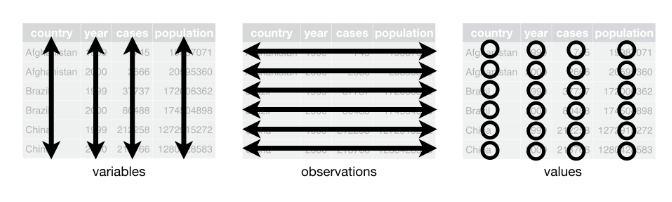
\includegraphics{img/05-tidy-principles.PNG}
\caption{\label{fig:unnamed-chunk-170}Tidy Data principles}
\end{figure}

Tidyverse is probably the most well-known package in the R community, but there is controversy behind it. High-profile people in the R community debate about whether \textbf{\texttt{tidyverse}} is actually appropriate for beginners to learn and whether it really is more effective and efficient than base R. Similarly, some of the R community dislike the idea that the \textbf{\texttt{tidyverse}} is the only ``real'' way to conduct data cleaning.

We will be using both base R and tidyverse in this course. The main thing that you should know is that tidyverse and Base R are like two different dialects in R. If in the future you search for help on R code, the code might be written from one perspective or the other. If the code looks more like what you saw in Chapters 2-4, then it is in base R. If you search for help and looks more like the code in the rest of the course, it's probably tidyverse.

Understanding both approaches will empower you to choose the one that aligns with your preferences and needs, ensuring you can find the right solution more effectively. Whether you are more comfortable with base R or tidyverse, knowing both approaches will enable you to navigate and utilize the wealth of resources available in the R community.

\hypertarget{lets-get-set-up}{%
\section{Let's Get Set Up}\label{lets-get-set-up}}

Okay, that's enough conceptual information for now - let's learn how to actually clean some data. First, we are going to need to get our RStudio or PositCloud environment ready. We'll do this by setting up our working directory, downloading and importing our data files, and then installing and loading the \texttt{tidyverse} packages.

\hypertarget{activity-1.1-set-up-your-wd}{%
\subsection{Activity 1.1: Set up your WD}\label{activity-1.1-set-up-your-wd}}

Remember that the working directory is the location where we want to store any resulting data files or scripts that you'll work on in a session. In Chapter 2 I showed you how to do this using \protect\hyperlink{set_wd}{a button-and-click interface}.

Using those instructions, create a folder called ``Week4'' in the \texttt{rintro} project folder (or whatever folder you created) and set it as your working directory. Use the ´getwd()´ to check that it has been set as your working directory. Your output should be something like this:

\begin{Shaded}
\begin{Highlighting}[]
\SpecialCharTok{\textgreater{}} \FunctionTok{setwd}\NormalTok{(}\StringTok{"C:/Users/0131045s/Desktop/Programming/R/Workshops/Example/Rintro\_2024/week4"}\NormalTok{)}
\end{Highlighting}
\end{Shaded}

\hypertarget{activity-1.2-import-your-csv-files-and-r-script}{%
\subsection{Activity 1.2: Import your CSV files and R script}\label{activity-1.2-import-your-csv-files-and-r-script}}

You need to import several files for this activity:

\begin{enumerate}
\def\labelenumi{\arabic{enumi}.}
\item
  \textbf{raw\_remote\_associations.csv}
\item
  \textbf{data\_cleaning\_script.R}
\end{enumerate}

To download these files, navigate to the Teams channel for this course and access the ``Week 4 - Data Cleaning (Part I)'' channel. Once downloaded, use your file management system (File Explorer on Windows or Finder on Mac) to copy and paste these files into the ``Week4'' folder you created in Activity 1.1.

If you're using RStudio, you should see these files in your working directory within the Files pane. Open the R script (\textbf{data\_cleaning\_script.R}).

To import the raw\_remote\_associations.csv dataset into R, do the following:

\begin{enumerate}
\def\labelenumi{\arabic{enumi}.}
\tightlist
\item
  Click Environment in the Environment Pane -\textgreater{} Import Dataset -\textgreater{} From Text(base) -\textgreater{} Select \textbf{raw\_remote\_associations.csv -\textgreater{}} change its name to \textbf{df\_raw}
\item
  \protect\hyperlink{importing}{See last week's section on importing data for more information}
\end{enumerate}

Alternatively, you can run the following command within the \textbf{data\_cleaning\_script.R}

\begin{Shaded}
\begin{Highlighting}[]
\NormalTok{df\_raw }\OtherTok{\textless{}{-}} \FunctionTok{read.csv}\NormalTok{(}\StringTok{"datasets/raw\_remote\_associations.csv"}\NormalTok{) }
\end{Highlighting}
\end{Shaded}

\hypertarget{activity-1.3-install-and-load-the-tidyverse-package}{%
\subsection{Activity 1.3: Install and load the tidyverse package}\label{activity-1.3-install-and-load-the-tidyverse-package}}

A good practice in R is to load packages at the start of your script. In the downloaded R script, you'll find the following lines commented out. Copy and paste the code \textbf{\texttt{install.packages("tidyverse")}} into your console and press enter to download the tidyverse package.

\begin{Shaded}
\begin{Highlighting}[]
\CommentTok{\#install.packages("tidyverse")}
\CommentTok{\#library(tidyverse)}
\end{Highlighting}
\end{Shaded}

\begin{figure}
\centering
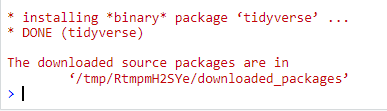
\includegraphics{img/05-tidyverse-install.PNG}
\caption{\label{fig:unnamed-chunk-175}Tidyverse Installation}
\end{figure}

Once installed, uncomment and run the \textbf{\texttt{library(tidyverse)}} in your script to load the package. If installed correctly, you should see the tidyverse package and its dependencies listed in the console. Since tidyverse contains multiple packages, it will load them all at once. So if you see the following then you are good to go.

\begin{Shaded}
\begin{Highlighting}[]
\FunctionTok{library}\NormalTok{(tidyverse)}
\end{Highlighting}
\end{Shaded}

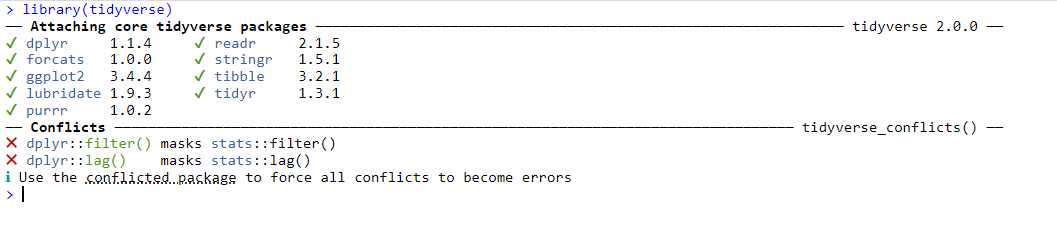
\includegraphics{img/05-tidyverse-message.PNG}

You might also get the following warnings when you load in R. If you do, that just means you are using an older version of R. At the beginning of the class, we downloaded version 4.2 onto our own computers, but in the meantime version 4.3 has been released. We can stick with our current version for now.

\begin{Shaded}
\begin{Highlighting}[]
\NormalTok{Warning}\SpecialCharTok{:}\NormalTok{ package ‘tidyverse’ was built under R version }\DecValTok{4}\NormalTok{.}\FloatTok{3.2}
\NormalTok{Warning}\SpecialCharTok{:}\NormalTok{ package ‘ggplot2’ was built under R version }\DecValTok{4}\NormalTok{.}\FloatTok{3.2}
\NormalTok{Warning}\SpecialCharTok{:}\NormalTok{ package ‘tibble’ was built under R version }\DecValTok{4}\NormalTok{.}\FloatTok{3.2}
\NormalTok{Warning}\SpecialCharTok{:}\NormalTok{ package ‘tidyr’ was built under R version }\DecValTok{4}\NormalTok{.}\FloatTok{3.2}
\NormalTok{Warning}\SpecialCharTok{:}\NormalTok{ package ‘readr’ was built under R version }\DecValTok{4}\NormalTok{.}\FloatTok{3.2}
\NormalTok{Warning}\SpecialCharTok{:}\NormalTok{ package ‘purrr’ was built under R version }\DecValTok{4}\NormalTok{.}\FloatTok{3.2}
\NormalTok{Warning}\SpecialCharTok{:}\NormalTok{ package ‘dplyr’ was built under R version }\DecValTok{4}\NormalTok{.}\FloatTok{3.2}
\NormalTok{Warning}\SpecialCharTok{:}\NormalTok{ package ‘stringr’ was built under R version }\DecValTok{4}\NormalTok{.}\FloatTok{3.2}
\NormalTok{Warning}\SpecialCharTok{:}\NormalTok{ package ‘forcats’ was built under R version }\DecValTok{4}\NormalTok{.}\FloatTok{3.2}
\NormalTok{Warning}\SpecialCharTok{:}\NormalTok{ package ‘lubridate’ was built under R version }\DecValTok{4}\NormalTok{.}\FloatTok{3.2}
\end{Highlighting}
\end{Shaded}

\hypertarget{cleaning-the-remote-associates-data-set.}{%
\section{Cleaning the Remote Associates Data set.}\label{cleaning-the-remote-associates-data-set.}}

\hypertarget{context-and-viewing-it-in-rstudio}{%
\subsection{Context and Viewing it in RStudio}\label{context-and-viewing-it-in-rstudio}}

The dataset we imported and are cleaning today comes from a study investigating the effect of mood induction on convergent thinking. Participants were required to read three emotional vignettes (one positive, one negative, and one neutral) before completing a remote associations test. In this test, 41 participants had to identify the link between given words (e.g., Square / Cardboard / Open, with the answer being ``Box''). The order of the vignettes was counterbalanced across participants. Additionally, participants completed five items on Openness from the Big Five Aspects, as it is known to positively correlate with convergent thinking.

The first step after importing a dataset is to check it to ensure that we have imported the correct data. We can do this using the \textbf{\texttt{head()}} function:

\begin{Shaded}
\begin{Highlighting}[]
\CommentTok{\#View(df\_raw) to open a new tab in Source and look at the entire dataset}
\FunctionTok{head}\NormalTok{(df\_raw) }\CommentTok{\#this will load the first six rows into the console}
\end{Highlighting}
\end{Shaded}

\begin{verbatim}
##   X Participant.Private.ID Local.Timestamp Experiment.Status
## 1 1               10168827     1.70601e+12           preview
## 2 2               10192092     1.70601e+12           preview
## 3 3               10205485     1.70601e+12           preview
## 4 4               10208522     1.70601e+12           preview
## 5 5               10218310     1.70601e+12           preview
## 6 6               10225898     1.70601e+12           preview
##   remote.assocotations.1 remote.assocotations.2 order Remote.association.3
## 1                      6                     13   ABC                   22
## 2                      9                     18   ABC                   27
## 3                      6                      6   BCA                    6
## 4                      3                     10   ABC                   18
## 5                      9                     18   CAB                   27
## 6                      3                      7   ABC                   11
##   Response Participant.OS response1 open1 open2 open3 open4 open5 age gender
## 1      END     Windows 10        50     3     3     3     3     3  34   male
## 2    BEGIN     Windows 10        63     3     4     3     3     3  34 female
## 3     bank     Windows 10        73     2     4     4     3     3  18   male
## 4      day     Windows 10        58     3     3     2     2     3  29 female
## 5    black     Windows 10        68     3     3     2     3     2  46   male
## 6   common     Windows 10        54     2     3     3     2     3  40 female
\end{verbatim}

Ouch! Now that is a data set only a parent could love. Here is what each column is telling us about each participant

\begin{longtable}[]{@{}
  >{\raggedright\arraybackslash}p{(\columnwidth - 2\tabcolsep) * \real{0.2500}}
  >{\raggedright\arraybackslash}p{(\columnwidth - 2\tabcolsep) * \real{0.7500}}@{}}
\toprule\noalign{}
\begin{minipage}[b]{\linewidth}\raggedright
Column
\end{minipage} & \begin{minipage}[b]{\linewidth}\raggedright
Description
\end{minipage} \\
\midrule\noalign{}
\endhead
\bottomrule\noalign{}
\endlastfoot
X & An empty column that counts the row number. \\
Participant.Private.ID & Experiment ID. \\
Local.Timestamp & Timestamp indicating when participants took part in the study. \\
Experiment.Status & Indicates whether the study was published (live) or not (preview) for each participant. \\
Remote-Associations1-3 & Scores on each remote associations task. \\
order & Order of watching the vignettes (A = ``positive'', B = ``negative'', C = ``neutral''). \\
Response & Participants' answers on the remote associations task. \\
Participant.OS & Operating system used by participants. \\
response1 & Aggregated mood score. \\
open1-open5 & Scores on Openness items. \\
age and gender & Participants' age and gender. \\
\end{longtable}

However, several issues are evident in this dataset:

\begin{enumerate}
\def\labelenumi{\arabic{enumi}.}
\item
  \textbf{Pointless columns:} Columns such as ``Local.Timestamp'' and ``Participant.OS'' are unnecessary for our analysis.
\item
  \textbf{Awkward, inconsistent, or misspelled column names:} Columns like ``Participant.Private.ID'' and ``remote.assocotations.2'' have awkward or misspelled names.
\item
  \textbf{Column order:} The order of columns is not ideal, with important columns scattered throughout the dataset.
\item
  \textbf{Improper scoring:} The maximum score on each remote association task in this study was 9. However, we have several scores that exceed this maximum value.
\item
  \textbf{Mismatch in participant count:} The dataset reports a different number of participants who completed the experiment (52) than what was expected (41).
\item
  \textbf{Presence of preview data:} The dataset contains responses from both the preview and live phases of the study, which need to be addressed by removing preview data.
\end{enumerate}

\hypertarget{key-functions-that-will-help-you-clean-most-datasets}{%
\subsection{Key Functions That Will Help You Clean Most Datasets}\label{key-functions-that-will-help-you-clean-most-datasets}}

The following functions are extremely useful for cleaning data frame in R. They all come from the \texttt{tidyverse} package. The following table defines each package and what it does. We will use each function in this chapter to clean the \texttt{remote\_associations} data frame, so you will get to practice each one.

\begin{longtable}[]{@{}
  >{\centering\arraybackslash}p{(\columnwidth - 2\tabcolsep) * \real{0.6620}}
  >{\raggedright\arraybackslash}p{(\columnwidth - 2\tabcolsep) * \real{0.3380}}@{}}
\toprule\noalign{}
\begin{minipage}[b]{\linewidth}\centering
Function
\end{minipage} & \begin{minipage}[b]{\linewidth}\raggedright
Description
\end{minipage} \\
\midrule\noalign{}
\endhead
\bottomrule\noalign{}
\endlastfoot
\href{https://dplyr.tidyverse.org/reference/select.html}{\texttt{select()}} & Include or exclude certain variables (columns) \\
\href{https://dplyr.tidyverse.org/reference/filter.html}{\texttt{filter()}} & Include or exclude certain observations (rows) \\
\href{https://dplyr.tidyverse.org/reference/mutate.html}{\texttt{mutate()}} & Create new variables (columns) \\
\href{https://dplyr.tidyverse.org/reference/arrange.html}{\texttt{arrange()}} & Change the order of observations (rows) \\
\href{https://dplyr.tidyverse.org/reference/group_by.html}{\texttt{group\_by()}} & Organize the observations (rows) into groups \\
\href{https://dplyr.tidyverse.org/reference/summarise.html}{\texttt{summarise()}} & Create summary variables for groups of observations \\
\href{https://dplyr.tidyverse.org/articles/base.html?q=distinct\#distinct-select-distinctunique-rows}{disinct()} & Select unique observations (rows) \\
\href{https://dplyr.tidyverse.org/articles/base.html?q=rename\#rename-rename-variables-by-name}{rename()} & Rename variables (columns) \\
\end{longtable}

\hypertarget{choosing-our-columns-of-interest-with-select}{%
\section{\texorpdfstring{Choosing our Columns of Interest with \texttt{Select()}}{Choosing our Columns of Interest with Select()}}\label{choosing-our-columns-of-interest-with-select}}

When you are first cleaning a data set, the first thing you should do is identify the columns that you might need in your analysis or hold important information. In our cases, these columns would be \texttt{Participant.Private.ID}, \texttt{Experiment.Status}, the response, remote associations, openness, and demographic columns. We can select those columns by using the \texttt{select()} function.

The formula for this function is: \texttt{select(dataframe,\ c(col1name,\ col2name,\ col3name))}

\begin{Shaded}
\begin{Highlighting}[]
\NormalTok{df\_select }\OtherTok{\textless{}{-}} \FunctionTok{select}\NormalTok{(df\_raw, }\FunctionTok{c}\NormalTok{(Participant.Private.ID, Experiment.Status, order,}
\NormalTok{                              remote.assocotations}\FloatTok{.1}\NormalTok{, remote.assocotations}\FloatTok{.2}\NormalTok{,   Remote.association}\FloatTok{.3}\NormalTok{, Response, response1, open1}\SpecialCharTok{:}\NormalTok{ gender))}

\FunctionTok{head}\NormalTok{(df\_select)}
\end{Highlighting}
\end{Shaded}

\begin{verbatim}
##   Participant.Private.ID Experiment.Status order remote.assocotations.1
## 1               10168827           preview   ABC                      6
## 2               10192092           preview   ABC                      9
## 3               10205485           preview   BCA                      6
## 4               10208522           preview   ABC                      3
## 5               10218310           preview   CAB                      9
## 6               10225898           preview   ABC                      3
##   remote.assocotations.2 Remote.association.3 Response response1 open1 open2
## 1                     13                   22      END        50     3     3
## 2                     18                   27    BEGIN        63     3     4
## 3                      6                    6     bank        73     2     4
## 4                     10                   18      day        58     3     3
## 5                     18                   27    black        68     3     3
## 6                      7                   11   common        54     2     3
##   open3 open4 open5 age gender
## 1     3     3     3  34   male
## 2     3     3     3  34 female
## 3     4     3     3  18   male
## 4     2     2     3  29 female
## 5     2     3     2  46   male
## 6     3     2     3  40 female
\end{verbatim}

Instantly, that is immediately better. Now there is a couple of things you might have noticed in my code.

The first is that the order in which I put columns in \texttt{select()} is the order in which the columns appear in the \texttt{df\_select}. This is a very useful feature of \texttt{select()} as it means we can reorder our dataframe and select the columns at the same time. Just to demonstrate this further.

\begin{Shaded}
\begin{Highlighting}[]
\NormalTok{df\_select }\OtherTok{\textless{}{-}} \FunctionTok{select}\NormalTok{(df\_select, Participant.Private.ID, Experiment.Status, age, gender, order, remote.assocotations}\FloatTok{.1}\SpecialCharTok{:}\NormalTok{open5)}

\FunctionTok{head}\NormalTok{(df\_select)}
\end{Highlighting}
\end{Shaded}

\begin{verbatim}
##   Participant.Private.ID Experiment.Status age gender order
## 1               10168827           preview  34   male   ABC
## 2               10192092           preview  34 female   ABC
## 3               10205485           preview  18   male   BCA
## 4               10208522           preview  29 female   ABC
## 5               10218310           preview  46   male   CAB
## 6               10225898           preview  40 female   ABC
##   remote.assocotations.1 remote.assocotations.2 Remote.association.3 Response
## 1                      6                     13                   22      END
## 2                      9                     18                   27    BEGIN
## 3                      6                      6                    6     bank
## 4                      3                     10                   18      day
## 5                      9                     18                   27    black
## 6                      3                      7                   11   common
##   response1 open1 open2 open3 open4 open5
## 1        50     3     3     3     3     3
## 2        63     3     4     3     3     3
## 3        73     2     4     4     3     3
## 4        58     3     3     2     2     3
## 5        68     3     3     2     3     2
## 6        54     2     3     3     2     3
\end{verbatim}

The second thing you might notice is that inside the \texttt{c} function I go from naming each column one at a time to using the \texttt{:} operator. If you remember from Chapters 3 \& 4, when you are selecting elements from a data structure, the \texttt{:} operator enables you to select anything between those elements. So the code \texttt{remote.assoctations.1:open5} selects every column starting from \texttt{remote.assoctations1} and ending with \texttt{open5}. This saves us from having to type out every column.

What if we wanted to remove one or two columns? Is there an easier way to remove them then by specifying the columns we want? Yes! We can use \texttt{select()} to remove columns. All we need to do is put the \texttt{-} operator before the column we want to remove.

If you look at the \texttt{Response} column, it doesn't really provide us with any genuinely useful information - we already have their performance on the task. So let's get rid of it.

\begin{Shaded}
\begin{Highlighting}[]
\NormalTok{df\_select }\OtherTok{\textless{}{-}} \FunctionTok{select}\NormalTok{(df\_select, }\SpecialCharTok{{-}}\NormalTok{Response) }\CommentTok{\#this will remove the \#response column}
\FunctionTok{head}\NormalTok{(df\_select)}
\end{Highlighting}
\end{Shaded}

\begin{verbatim}
##   Participant.Private.ID Experiment.Status age gender order
## 1               10168827           preview  34   male   ABC
## 2               10192092           preview  34 female   ABC
## 3               10205485           preview  18   male   BCA
## 4               10208522           preview  29 female   ABC
## 5               10218310           preview  46   male   CAB
## 6               10225898           preview  40 female   ABC
##   remote.assocotations.1 remote.assocotations.2 Remote.association.3 response1
## 1                      6                     13                   22        50
## 2                      9                     18                   27        63
## 3                      6                      6                    6        73
## 4                      3                     10                   18        58
## 5                      9                     18                   27        68
## 6                      3                      7                   11        54
##   open1 open2 open3 open4 open5
## 1     3     3     3     3     3
## 2     3     4     3     3     3
## 3     2     4     4     3     3
## 4     3     3     2     2     3
## 5     3     3     2     3     2
## 6     2     3     3     2     3
\end{verbatim}

\hypertarget{renaming-our-columns-of-interest-with-rename}{%
\section{\texorpdfstring{Renaming our Columns of Interest with \texttt{rename()}}{Renaming our Columns of Interest with rename()}}\label{renaming-our-columns-of-interest-with-rename}}

Our data set is definitely looking cleaner after having shedding those columns, but good grief are those names still ugly. Luckily, we can change their name using the \texttt{rename()} function. The syntax for this function is slightly counter intuitive in its order, as it goes like this: \texttt{rename(df,\ newcolumnane\ =\ oldcolumnname)}

\begin{Shaded}
\begin{Highlighting}[]
\NormalTok{df\_rename }\OtherTok{\textless{}{-}} \FunctionTok{rename}\NormalTok{(df\_select, }
                    \AttributeTok{ID =}\NormalTok{ Participant.Private.ID, }\CommentTok{\#newcolname = oldcolname}
                    \AttributeTok{status =}\NormalTok{ Experiment.Status,}
                    \AttributeTok{remote\_pos =}\NormalTok{ remote.assocotations}\FloatTok{.1}\NormalTok{,}
                    \AttributeTok{remote\_neg =}\NormalTok{ remote.assocotations}\FloatTok{.2}\NormalTok{,}
                    \AttributeTok{remote\_neut =}\NormalTok{ Remote.association}\FloatTok{.3}\NormalTok{,}
                    \AttributeTok{total\_mood =}\NormalTok{ response1,}
                    \AttributeTok{condition =}\NormalTok{ order)}

\FunctionTok{head}\NormalTok{(df\_rename)}
\end{Highlighting}
\end{Shaded}

\begin{verbatim}
##         ID  status age gender condition remote_pos remote_neg remote_neut
## 1 10168827 preview  34   male       ABC          6         13          22
## 2 10192092 preview  34 female       ABC          9         18          27
## 3 10205485 preview  18   male       BCA          6          6           6
## 4 10208522 preview  29 female       ABC          3         10          18
## 5 10218310 preview  46   male       CAB          9         18          27
## 6 10225898 preview  40 female       ABC          3          7          11
##   total_mood open1 open2 open3 open4 open5
## 1         50     3     3     3     3     3
## 2         63     3     4     3     3     3
## 3         73     2     4     4     3     3
## 4         58     3     3     2     2     3
## 5         68     3     3     2     3     2
## 6         54     2     3     3     2     3
\end{verbatim}

\hypertarget{creating-new-columns-using-the-mutate-function}{%
\section{\texorpdfstring{Creating new Columns using the \texttt{mutate()} function}{Creating new Columns using the mutate() function}}\label{creating-new-columns-using-the-mutate-function}}

Okay, so we have gotten rid of superfluous columns and cleaned up the names of the ones we have left. But there is still a column ``missing''. At the moment, we have participants' scores on individual items for Openness to Experience. But unless we are running a reliability or factor analysis, we actually want participants' total level of openness.

The \textbf{\texttt{mutate()}} function will help us create that column. This function takes existing column(s) and performs operations on them to create new columns in our data set.

Let's use \textbf{\texttt{mutate()}} to create a column called \textbf{\texttt{total\_openness}}. The syntax for this function is: \textbf{\texttt{mutate(df,\ new\_column\_name\ =\ instructions\ on\ what\ to\ do\ with\ current\ columns)}}

\begin{Shaded}
\begin{Highlighting}[]
\NormalTok{df\_mutate }\OtherTok{\textless{}{-}} \FunctionTok{mutate}\NormalTok{(df\_rename, }
                    \AttributeTok{total\_openness =}\NormalTok{ open1 }\SpecialCharTok{+}\NormalTok{ open2 }\SpecialCharTok{+}\NormalTok{ open3 }\SpecialCharTok{+}\NormalTok{ open4 }\SpecialCharTok{+}\NormalTok{ open5)}
                    \CommentTok{\#new\_col\_name = operation on current columns}

\NormalTok{df\_mutate}\SpecialCharTok{$}\NormalTok{total\_openness}
\end{Highlighting}
\end{Shaded}

\begin{verbatim}
##  [1] 15 16 16 13 13 13 16 14 14 14 14 15 14 15 14 14 16 14 15 15 18 14 17 14 16
## [26] 15 16 15 16 15 16 16 15 15 16 17 15 17 15 15 15 17 16 14 13 15 17 14 14 14
## [51] 17
\end{verbatim}

If we wanted to calculate the mean of these items, then the process is slightly more complicated. First, we would need to tell R that we want the mean per observation rather than per column (e.g., we need the mean score of open1 to open5 per participant, rather than across the entire dataset) by using the \textbf{\texttt{rowMeans()}} function. Then we would need to \textbf{\texttt{select()}} the columns that we want the row means from.

Let's do this and save the operation to a new column called \textbf{\texttt{mean\_openness}}

\begin{Shaded}
\begin{Highlighting}[]
\NormalTok{df\_mutate }\OtherTok{\textless{}{-}} \FunctionTok{mutate}\NormalTok{(df\_mutate, }
                    \CommentTok{\#we use \textasciigrave{}select()\textasciigrave{} to pick the columns we want}
                    \AttributeTok{mean\_openness =} \FunctionTok{rowMeans}\NormalTok{(}\FunctionTok{select}\NormalTok{(df\_mutate, }
                                                    \FunctionTok{c}\NormalTok{(open1, open2, open3,}
\NormalTok{                                                      open4, open5))))}
                    

\FunctionTok{head}\NormalTok{(df\_mutate)}
\end{Highlighting}
\end{Shaded}

\begin{verbatim}
##         ID  status age gender condition remote_pos remote_neg remote_neut
## 1 10168827 preview  34   male       ABC          6         13          22
## 2 10192092 preview  34 female       ABC          9         18          27
## 3 10205485 preview  18   male       BCA          6          6           6
## 4 10208522 preview  29 female       ABC          3         10          18
## 5 10218310 preview  46   male       CAB          9         18          27
## 6 10225898 preview  40 female       ABC          3          7          11
##   total_mood open1 open2 open3 open4 open5 total_openness mean_openness
## 1         50     3     3     3     3     3             15           3.0
## 2         63     3     4     3     3     3             16           3.2
## 3         73     2     4     4     3     3             16           3.2
## 4         58     3     3     2     2     3             13           2.6
## 5         68     3     3     2     3     2             13           2.6
## 6         54     2     3     3     2     3             13           2.6
\end{verbatim}

If we do not need the individual items, then there is an argument in \textbf{\texttt{mutate()}} called \textbf{\texttt{.keep}}. This specifies what should be done with the columns that were operated on to create the new column. If this argument is set to \textbf{\texttt{unused}}, then R will only keep columns that were not used to create the new column. In other words, it will remove any columns used to calculate the new column.

\begin{Shaded}
\begin{Highlighting}[]
\NormalTok{df\_mutate }\OtherTok{\textless{}{-}} \FunctionTok{mutate}\NormalTok{(df\_rename, }
                    \AttributeTok{total\_openness =}\NormalTok{ open1 }\SpecialCharTok{+}\NormalTok{ open2 }\SpecialCharTok{+}\NormalTok{ open3 }\SpecialCharTok{+}\NormalTok{ open4 }\SpecialCharTok{+}\NormalTok{ open5,}
                    \AttributeTok{.keep =} \StringTok{"unused"}\NormalTok{)}

\FunctionTok{head}\NormalTok{(df\_mutate)}
\end{Highlighting}
\end{Shaded}

\begin{verbatim}
##         ID  status age gender condition remote_pos remote_neg remote_neut
## 1 10168827 preview  34   male       ABC          6         13          22
## 2 10192092 preview  34 female       ABC          9         18          27
## 3 10205485 preview  18   male       BCA          6          6           6
## 4 10208522 preview  29 female       ABC          3         10          18
## 5 10218310 preview  46   male       CAB          9         18          27
## 6 10225898 preview  40 female       ABC          3          7          11
##   total_mood total_openness
## 1         50             15
## 2         63             16
## 3         73             16
## 4         58             13
## 5         68             13
## 6         54             13
\end{verbatim}

\hypertarget{rewriting-existing-columns-using-mutate}{%
\subsection{\texorpdfstring{Rewriting existing columns using \texttt{mutate()}}{Rewriting existing columns using mutate()}}\label{rewriting-existing-columns-using-mutate}}

If we have a column that contains mistakes, we can use \textbf{\texttt{mutate()}} to rewrite that column's values. The syntax for this is the same as when you are creating new columns with \textbf{\texttt{mutate}}: \textbf{\texttt{mutate(df,\ existing\_column\_name\ =\ instructions\ on\ what\ to\ do\ with\ current\ columns)}}

If you look at our columns \textbf{\texttt{remote\_pos}}, \textbf{\texttt{remote\_neg}}, and \textbf{\texttt{remote\_neut}}, there is a mistake. Each column should represent the participants' scores (out of a maximum score of 9) on the remote associations task after engaging with either positive, negative, or neutral stimuli. However, while \textbf{\texttt{remote\_pos}} scoring looks correct, the scores for \textbf{\texttt{remote\_neg}} are going up to 18, and the scores for \textbf{\texttt{remote\_neut}} are going up to 27. So what is going on?

What happened here is that Gorilla Research added participants' scores on each task to each other. So the \textbf{\texttt{remote\_neg}} column is really the participants' correct answers on \textbf{\texttt{remote\_pos}} plus their correct answers on \textbf{\texttt{remote\_neg}}. Similarly, the \textbf{\texttt{remote\_neut}} contains their scores on the \textbf{\texttt{remote\_neg}} column plus their scores on the \textbf{\texttt{remote\_neut}} task.

To fix this, the formula we need to use is the following:

\begin{enumerate}
\def\labelenumi{\arabic{enumi}.}
\item
  remote\_neg = remote\_neg - remote\_pos
\item
  remote\_neut = remote\_neut - remote\_neg
\end{enumerate}

We can fix this error using the \textbf{\texttt{mutate()}} function

\begin{Shaded}
\begin{Highlighting}[]
\NormalTok{df\_mutate\_ra }\OtherTok{\textless{}{-}} \FunctionTok{mutate}\NormalTok{(df\_mutate, }
                    \AttributeTok{remote\_neg =}\NormalTok{ remote\_neg }\SpecialCharTok{{-}}\NormalTok{ remote\_pos,}
                    \AttributeTok{remote\_neut =}\NormalTok{ remote\_neut }\SpecialCharTok{{-}}\NormalTok{ remote\_neg)}

\FunctionTok{head}\NormalTok{(df\_mutate\_ra)}
\end{Highlighting}
\end{Shaded}

\begin{verbatim}
##         ID  status age gender condition remote_pos remote_neg remote_neut
## 1 10168827 preview  34   male       ABC          6          7          15
## 2 10192092 preview  34 female       ABC          9          9          18
## 3 10205485 preview  18   male       BCA          6          0           6
## 4 10208522 preview  29 female       ABC          3          7          11
## 5 10218310 preview  46   male       CAB          9          9          18
## 6 10225898 preview  40 female       ABC          3          4           7
##   total_mood total_openness
## 1         50             15
## 2         63             16
## 3         73             16
## 4         58             13
## 5         68             13
## 6         54             13
\end{verbatim}

Hold on, what happened here? The \textbf{\texttt{remote\_neut}} scores are still 9+? Well, we first changed the column \textbf{\texttt{remote\_neg}} to get our correct scores on this task. However, the new values of \textbf{\texttt{remote\_neg}} are then inserted on the next line of the formula. To fix for this error, we need to put \textbf{\texttt{remote\_neut}} first

\begin{Shaded}
\begin{Highlighting}[]
\NormalTok{df\_mutate\_ra\_fixed }\OtherTok{\textless{}{-}} \FunctionTok{mutate}\NormalTok{(df\_mutate,}
                    \AttributeTok{remote\_neut =}\NormalTok{  remote\_neut }\SpecialCharTok{{-}}\NormalTok{ remote\_neg,}
                    \AttributeTok{remote\_neg =}\NormalTok{ remote\_neg }\SpecialCharTok{{-}}\NormalTok{ remote\_pos)}

\NormalTok{df\_mutate\_ra\_fixed}\SpecialCharTok{$}\NormalTok{remote\_neut}
\end{Highlighting}
\end{Shaded}

\begin{verbatim}
##  [1]  9  9  0  8  9  4  9  5  9  2  1  9  6  7  9 28  4  8  9  7  0  4  9  9  9
## [26]  8  5  9  6  6  0  9  0  4  5  0  7  1  1  5  6  9  9  0  8  3  0  9  8  9
## [51]  1
\end{verbatim}

Better!

\hypertarget{checking-in-on-our-data-set}{%
\section{Checking in on our data set}\label{checking-in-on-our-data-set}}

We've done a good bit of cleaning so far. We have removed unnecessary columns, we have fixed their names and their order, we have created new columns, and we have fixed errors in existing columns. Our data set is looking nearly ready for analysis.

However, there is still data that needs to be removed. We should only have 41 participants in our sample, but if you look at your dataframe, we actually have 51 participants.

\begin{Shaded}
\begin{Highlighting}[]
\FunctionTok{nrow}\NormalTok{(df\_mutate\_ra\_fixed)}
\end{Highlighting}
\end{Shaded}

\begin{verbatim}
## [1] 51
\end{verbatim}

So where are these extra 10 participants coming from? If you look in the \textbf{\texttt{status}} column in our data set, you'll notice that there exists both \textbf{\texttt{preview}} and \textbf{\texttt{live}} data. We can use the \textbf{\texttt{table()}} function to count the number of participants who contributed \textbf{\texttt{preview}} versus \textbf{\texttt{live}} data.

\begin{Shaded}
\begin{Highlighting}[]
\FunctionTok{table}\NormalTok{(df\_mutate\_ra\_fixed}\SpecialCharTok{$}\NormalTok{status)}
\end{Highlighting}
\end{Shaded}

\begin{verbatim}
## 
##    live preview 
##      42       9
\end{verbatim}

Okay, so 9 of our extra 10 participants are coming from preview data. That means we have one extra participant than we should have from when we published the study. The first thing we should do is check what is going on here.

After that, we'll need to remove the 9 preview participants from the dataframe.

The following operations will enable us to clean our datasets based on participant scores on a row-by-row basis rather than on a column basis.

\hypertarget{removing-duplicates-using-distinct}{%
\section{\texorpdfstring{Removing Duplicates using \texttt{distinct()}}{Removing Duplicates using distinct()}}\label{removing-duplicates-using-distinct}}

What could explain the extra participant? Well, there may have been an error when we downloaded the data and rows got duplicated. Luckily, there is a relatively easy way to do this through the \textbf{\texttt{duplicated()}} function. We call the function and give it the dataframe we want to check. The function then checks each row to see if it is a duplicate of another row.

\begin{Shaded}
\begin{Highlighting}[]
\FunctionTok{duplicated}\NormalTok{(df\_mutate\_ra\_fixed)}
\end{Highlighting}
\end{Shaded}

\begin{verbatim}
##  [1] FALSE FALSE FALSE FALSE FALSE FALSE FALSE FALSE FALSE FALSE FALSE FALSE
## [13] FALSE FALSE FALSE FALSE FALSE FALSE FALSE FALSE FALSE FALSE FALSE FALSE
## [25] FALSE FALSE FALSE FALSE FALSE FALSE FALSE FALSE FALSE FALSE FALSE FALSE
## [37] FALSE FALSE FALSE FALSE FALSE FALSE FALSE FALSE FALSE FALSE FALSE FALSE
## [49] FALSE FALSE  TRUE
\end{verbatim}

The function prints out logical data types \textbf{\texttt{TRUE}} or \textbf{\texttt{FALSE}}. Each answer corresponds to a row in the \textbf{\texttt{df\_mutate\_ra\_fixed}} data frame. We can see that the last row is the only one with a value of \textbf{\texttt{TRUE}}, which means it is a duplicate of another row. If we want to extract and see the duplicated rows, we can follow the syntax we discussed in Chapter 3 about extracting values from a dataframe: \textbf{\texttt{dataframe{[}rows\_we\_want,\ columns\_we\_want{]}}}

\begin{Shaded}
\begin{Highlighting}[]
\NormalTok{df\_mutate\_ra\_fixed[}\FunctionTok{duplicated}\NormalTok{(df\_mutate\_ra\_fixed), ]}
\end{Highlighting}
\end{Shaded}

\begin{verbatim}
##          ID status age gender condition remote_pos remote_neg remote_neut
## 51 10230547   live  28 female       CAB          1          1           1
##    total_mood total_openness
## 51         64             17
\end{verbatim}

We can see that the participant with the \textbf{\texttt{ID\ =\ 10230547}} has a duplicated value. To remove these values we can use the \textbf{\texttt{distinct()}} function. This function takes in a data frame or a column and only keeps the rows that are unique.

\begin{Shaded}
\begin{Highlighting}[]
\NormalTok{df\_distinct }\OtherTok{\textless{}{-}} \FunctionTok{distinct}\NormalTok{(df\_mutate\_ra\_fixed)}
\end{Highlighting}
\end{Shaded}

We can use the \textbf{\texttt{table()}} function to check whether we have removed the extra participant.

\begin{Shaded}
\begin{Highlighting}[]
\FunctionTok{table}\NormalTok{(df\_distinct}\SpecialCharTok{$}\NormalTok{status)}
\end{Highlighting}
\end{Shaded}

\begin{verbatim}
## 
##    live preview 
##      41       9
\end{verbatim}

It looks like we have. We can also double-check this by calling the Similarly, if we used the \textbf{\texttt{duplicated()}} function again to see if any values return as \textbf{\texttt{TRUE}}

\begin{Shaded}
\begin{Highlighting}[]
\FunctionTok{duplicated}\NormalTok{(df\_distinct)}
\end{Highlighting}
\end{Shaded}

\begin{verbatim}
##  [1] FALSE FALSE FALSE FALSE FALSE FALSE FALSE FALSE FALSE FALSE FALSE FALSE
## [13] FALSE FALSE FALSE FALSE FALSE FALSE FALSE FALSE FALSE FALSE FALSE FALSE
## [25] FALSE FALSE FALSE FALSE FALSE FALSE FALSE FALSE FALSE FALSE FALSE FALSE
## [37] FALSE FALSE FALSE FALSE FALSE FALSE FALSE FALSE FALSE FALSE FALSE FALSE
## [49] FALSE FALSE
\end{verbatim}

There we go, we have successfully removed the duplicate from our data frame. Now let's handle the data that was collected when the study was being \texttt{previewed}.

\hypertarget{removing-rows-using-the-filter-function}{%
\section{\texorpdfstring{Removing Rows using the \texttt{filter()} Function}{Removing Rows using the filter() Function}}\label{removing-rows-using-the-filter-function}}

We can use the \textbf{\texttt{filter()}} function to selectively retain or discard rows in a dataset based on specified conditions. Its syntax is structured as follows: \textbf{\texttt{filter(dataframe,\ condition)}}, where the condition specifies which rows to retain.

In the case of our status column, suppose we want to retain only the rows where the status is ``live'' and remove those where it is ``preview''. We achieve this with the following code:

\begin{Shaded}
\begin{Highlighting}[]
\NormalTok{df\_filter }\OtherTok{\textless{}{-}} \FunctionTok{filter}\NormalTok{(df\_distinct, status }\SpecialCharTok{==} \StringTok{"live"}\NormalTok{)}
\end{Highlighting}
\end{Shaded}

The condition \textbf{\texttt{status\ ==\ "live"}} instructs R to retain rows where the status column equals \textbf{\texttt{"live"}}. Rows that do not meet this condition are filtered out (e.g., where \textbf{\texttt{status\ ==\ "preview"}}). We can use the \textbf{\texttt{table()}} function to check that we only have rows where \textbf{\texttt{status\ ==\ "live"}}

\begin{Shaded}
\begin{Highlighting}[]
\FunctionTok{table}\NormalTok{(df\_filter}\SpecialCharTok{$}\NormalTok{status)}
\end{Highlighting}
\end{Shaded}

\begin{verbatim}
## 
## live 
##   41
\end{verbatim}

We can also use negative conditions in \textbf{\texttt{filter()}}. By that, I mean we can tell R to keep rows that \textbf{\emph{do not}} meet a certain condition. For example, I will get the same resulting data set if I tell R to keep rows that are not equal to \textbf{\texttt{preview}} in the \textbf{\texttt{status}} column.

\begin{Shaded}
\begin{Highlighting}[]
\NormalTok{df\_filter\_neg }\OtherTok{\textless{}{-}} \FunctionTok{filter}\NormalTok{(df\_distinct, status }\SpecialCharTok{!=} \StringTok{"preview"}\NormalTok{)}

\FunctionTok{table}\NormalTok{(df\_filter\_neg}\SpecialCharTok{$}\NormalTok{status)}
\end{Highlighting}
\end{Shaded}

\begin{verbatim}
## 
## live 
##   41
\end{verbatim}

Here, \textbf{\texttt{!=}} denotes ``not equal to'', allowing us to exclude rows where the status is \textbf{\texttt{"preview"}}. This can be really useful if you have multiple answers within a column and it's easier to tell R what not to keep rather than specify everything it needs to keep.

Since we have removed the \textbf{\texttt{preview}} scores from our \textbf{\texttt{status}} column, do we actually need it anymore? Probably not as it won't be used in our final analysis. So let's remove it using the \textbf{\texttt{select()}} function and \textbf{\texttt{-}} operator.

\begin{Shaded}
\begin{Highlighting}[]
\NormalTok{df\_filter }\OtherTok{\textless{}{-}} \FunctionTok{select}\NormalTok{(df\_filter, }\SpecialCharTok{{-}}\NormalTok{status)}
\end{Highlighting}
\end{Shaded}

\hypertarget{removing-rows-using-multiple-conditions-with-filter}{%
\subsection{\texorpdfstring{Removing Rows Using Multiple Conditions with \texttt{filter()}}{Removing Rows Using Multiple Conditions with filter()}}\label{removing-rows-using-multiple-conditions-with-filter}}

We can also use \textbf{\texttt{filter()}} to check whether rows meet several conditions at the same time. For example, let's look at our columns \textbf{\texttt{remote\_pos}}, \textbf{\texttt{remote\_neg}}, and \textbf{\texttt{remote\_neut}} which corresponds to different times they completed the remote associations task. Participants could score a maximum of 9 and a minimum of 0 on each task.

We might expect that it is reasonable that any participant could score a 0 on a single remote association task. Similarly, we might conclude that it is reasonable that a participant scored a 0 on two remote associations tasks. But we might be suspicious if they scored 0 on all three remote associations tasks. This could be evidence that the participant wasn't paying attention and was just motoring through the study as quickly as possible.

We can use the \textbf{\texttt{arrange()}} function to check whether participants scored \textbf{\texttt{0}} on these columns. To use the \textbf{\texttt{arrange()}} function you specify the data frame, and then you specify the column or columns that you want to arrange by. The syntax is: \textbf{\texttt{arrange(df,\ col1,\ col2,\ col3)}}

The function arranges in ascending fashion by default (this can be overridden). If you specify multiple columns, it will arrange in the order of the columns you enter. The following code will arrange our dataframe first by the values of \textbf{\texttt{remote\_pos}}, then by \textbf{\texttt{remote\_neg}}, and then by \textbf{\texttt{remote\_neut}}.

\begin{Shaded}
\begin{Highlighting}[]
\NormalTok{df\_filter }\OtherTok{\textless{}{-}} \FunctionTok{arrange}\NormalTok{(df\_filter, remote\_pos, remote\_neg, remote\_neut)}

\FunctionTok{head}\NormalTok{(df\_filter)}
\end{Highlighting}
\end{Shaded}

\begin{verbatim}
##         ID age gender condition remote_pos remote_neg remote_neut total_mood
## 1 10229575  47 female       BCA          0          0           0         70
## 2 10230546  43 female       ABC          0          0           0         88
## 3 10230541  46   male       BCA          0          0           0         63
## 4 10229436  26   male       CAB          0          2           4         61
## 5 10230533  36 female       CAB          0          4           4         62
## 6 10230659  45 female       ABC          0          5           0         74
##   total_openness
## 1             15
## 2             17
## 3             14
## 4             16
## 5             15
## 6             17
\end{verbatim}

We can see that there are three participants scored a \textbf{\texttt{0}} on all three tasks. How could we remove these participants? Well, we can use \textbf{\texttt{filter()}} to individually check whether participants' scores on the relevant column were greater than 0 using the sign \textbf{\texttt{\textgreater{}}}. We could then save the results to different data frames.

\begin{Shaded}
\begin{Highlighting}[]
\NormalTok{df\_filter\_pos }\OtherTok{\textless{}{-}} \FunctionTok{filter}\NormalTok{(df\_filter, remote\_pos }\SpecialCharTok{\textgreater{}} \DecValTok{0}\NormalTok{) }\CommentTok{\#it will only keep rows in remote\_pos that are greater than 0}

\NormalTok{df\_filter\_neg }\OtherTok{\textless{}{-}} \FunctionTok{filter}\NormalTok{(df\_filter\_pos, remote\_neg }\SpecialCharTok{\textgreater{}} \DecValTok{0}\NormalTok{) }\CommentTok{\#this code will only keeps row in remote\_neg that are greater than 0}

\NormalTok{df\_filter\_neut }\OtherTok{\textless{}{-}} \FunctionTok{filter}\NormalTok{(df\_filter\_neg, remote\_neut }\SpecialCharTok{\textgreater{}} \DecValTok{0}\NormalTok{) }\CommentTok{\#this code will only keep rows in the remote\_neg that are greater than 0 }
\end{Highlighting}
\end{Shaded}

This gets the job done, but it is a tedious approach as we need to type out the same command three times. It makes it significantly more likely we will make a mistake somewhere too.

Luckily, we can do this all in the one line using the \textbar{} operator. The \textbar{} operator translates to the logical condition \textbf{\texttt{OR}}.

\begin{Shaded}
\begin{Highlighting}[]
\NormalTok{df\_filter\_multi }\OtherTok{\textless{}{-}} \FunctionTok{filter}\NormalTok{(df\_filter, remote\_pos }\SpecialCharTok{\textgreater{}} \DecValTok{0} \SpecialCharTok{|}\NormalTok{ remote\_neg }\SpecialCharTok{\textgreater{}} \DecValTok{0} \SpecialCharTok{|}\NormalTok{ remote\_neg }\SpecialCharTok{\textgreater{}} \DecValTok{0}\NormalTok{)}
\end{Highlighting}
\end{Shaded}

This code translates to ``Create a new variable called \textbf{\texttt{df\_filter\_multi}} by taking the \textbf{\texttt{df\_filter}} dataframe and keep only the rows where participants score higher than 0 on either remote\_pos, remote\_neg, and remote\_neut. If a participant scores 0 on ALL of these columns, please remove them.''

This removes any participants from our dataset that did not get a single correct answer on any of the three remote associations tasks. The \textbf{\texttt{nrow()}} function shows us that our manipulation was successful.

\begin{Shaded}
\begin{Highlighting}[]
\FunctionTok{nrow}\NormalTok{(df\_filter\_multi)}
\end{Highlighting}
\end{Shaded}

\begin{verbatim}
## [1] 38
\end{verbatim}

What if we wanted to be more strict? What if we wanted to remove any participant that scored a \textbf{\texttt{0}} on \textbf{\emph{any}} of \textbf{\texttt{remote\_pos}}, \textbf{\texttt{remote\_neg}}, \textbf{\texttt{remote\_neut}}? In this case, we can use the \textbf{\texttt{\&}} operator, which translates to the logical condition \textbf{\texttt{AND}}.

\begin{Shaded}
\begin{Highlighting}[]
\NormalTok{df\_filter\_multi\_strict }\OtherTok{\textless{}{-}} \FunctionTok{filter}\NormalTok{(df\_filter, remote\_pos }\SpecialCharTok{\textgreater{}} \DecValTok{0} \SpecialCharTok{\&}\NormalTok{ remote\_neg }\SpecialCharTok{\textgreater{}} \DecValTok{0} \SpecialCharTok{\&}\NormalTok{ remote\_neg }\SpecialCharTok{\textgreater{}} \DecValTok{0}\NormalTok{)}
\end{Highlighting}
\end{Shaded}

This code translates to: ``Create a new variable called \textbf{\texttt{df\_filter\_multi\_strict}} by taking the \textbf{\texttt{df\_filter}} dataframe and keeping only the rows that have a score that is greater than or equal (\textgreater=) to 0 on remote\_pos, remote\_neg, and remote\_neut. If a participant has a score of 0 on ANY of these columns, please remove them.''

If we check the number of rows again, we can see that our data frame has shrunk.

\begin{Shaded}
\begin{Highlighting}[]
\FunctionTok{nrow}\NormalTok{(df\_filter\_multi\_strict)}
\end{Highlighting}
\end{Shaded}

\begin{verbatim}
## [1] 33
\end{verbatim}

What if we wanted to be stricter again and say that we want to remove participants if they scored less than a 2 on any of the remote association columns? Well, we use the less than or equal to operator \textbf{\texttt{\textgreater{}=}}

\begin{Shaded}
\begin{Highlighting}[]
\NormalTok{df\_filter\_multi\_stricter }\OtherTok{\textless{}{-}} \FunctionTok{filter}\NormalTok{(df\_filter, remote\_pos }\SpecialCharTok{\textgreater{}=} \DecValTok{2} \SpecialCharTok{\&}\NormalTok{ remote\_neg }\SpecialCharTok{\textgreater{}=} \DecValTok{2} \SpecialCharTok{\&}\NormalTok{ remote\_neg }\SpecialCharTok{\textgreater{}=} \DecValTok{2}\NormalTok{)}
\end{Highlighting}
\end{Shaded}

This code will only keep participants who scored a 2 or higher in all three columns. If we check \textbf{\texttt{nrow()}}, we will see that our data frame has shrunk even further

\begin{Shaded}
\begin{Highlighting}[]
\FunctionTok{nrow}\NormalTok{(df\_filter\_multi\_stricter)}
\end{Highlighting}
\end{Shaded}

\begin{verbatim}
## [1] 26
\end{verbatim}

I am not a big fan of either the \texttt{df\_filter\_multi\_strict} or \texttt{df\_filter\_multi\_stricter} columns. So let's carry the \texttt{df\_filter\_multi} data frame to the next section.

\hypertarget{identifying-the-factors-in-our-data-frame}{%
\section{Identifying the Factors in our Data Frame}\label{identifying-the-factors-in-our-data-frame}}

In the last chapter, we talked about the \textbf{\texttt{factor}} data type, which enables us to identify different levels of a variable. This would be the equivalent of identifying which variables are \textbf{\texttt{nominal}} or \textbf{\texttt{ordinal}} in SPSS. It is important to specify which of your columns are factors when you are cleaning your data, as certain inferential tests require the factor data type as an input. If we look at our current columns, none of them are the \textbf{\texttt{factors}}.

\begin{Shaded}
\begin{Highlighting}[]
\FunctionTok{glimpse}\NormalTok{(df\_filter\_multi)}
\end{Highlighting}
\end{Shaded}

\begin{verbatim}
## Rows: 38
## Columns: 9
## $ ID             <int> 10229436, 10230533, 10230659, 10428518, 10229522, 10229~
## $ age            <int> 26, 36, 45, 37, 30, 36, 28, 47, 46, 35, 18, 20, 33, 28,~
## $ gender         <chr> "male", "female", "female", "male", "female", "female",~
## $ condition      <chr> "CAB", "CAB", "ABC", "BCA", "CAB", "ABC", "CAB", "ABC",~
## $ remote_pos     <int> 0, 0, 0, 0, 1, 1, 1, 1, 1, 1, 1, 2, 2, 2, 3, 3, 3, 4, 4~
## $ remote_neg     <int> 2, 4, 5, 9, 1, 1, 1, 1, 1, 2, 5, 0, 6, 8, 3, 5, 7, 4, 4~
## $ remote_neut    <int> 4, 4, 0, 9, 0, 1, 1, 1, 2, 28, 6, 0, 6, 8, 3, 5, 7, 4, ~
## $ total_mood     <int> 61, 62, 74, 68, 59, 63, 64, 75, 48, 52, 65, 70, 64, 48,~
## $ total_openness <int> 16, 15, 17, 14, 16, 14, 17, 15, 14, 14, 15, 18, 14, 14,~
\end{verbatim}

Let's say for this study, we were interested in investigating the effect of \textbf{\texttt{gender}} and \textbf{\texttt{condition}} on participants' performance. We would need to convert these two columns to factors. How could we do this? Well, if you remember, we can use \textbf{\texttt{as.factor()}} to convert a vector into a factor, and we can use \textbf{\texttt{mutate()}} to rewrite existing columns. Let's combine these two approaches now to turn \textbf{\texttt{gender}} and \textbf{\texttt{condition}} into factors.

\begin{Shaded}
\begin{Highlighting}[]
\NormalTok{df\_factor }\OtherTok{\textless{}{-}} \FunctionTok{mutate}\NormalTok{(df\_filter\_multi,}
                    \AttributeTok{gender =} \FunctionTok{as.factor}\NormalTok{(gender),}
                    \AttributeTok{condition =} \FunctionTok{as.factor}\NormalTok{(condition))}
\end{Highlighting}
\end{Shaded}

Now if we call \textbf{\texttt{glimpse()}}, we will see that these columns are now factors.

\begin{Shaded}
\begin{Highlighting}[]
\FunctionTok{glimpse}\NormalTok{(df\_factor)}
\end{Highlighting}
\end{Shaded}

\begin{verbatim}
## Rows: 38
## Columns: 9
## $ ID             <int> 10229436, 10230533, 10230659, 10428518, 10229522, 10229~
## $ age            <int> 26, 36, 45, 37, 30, 36, 28, 47, 46, 35, 18, 20, 33, 28,~
## $ gender         <fct> male, female, female, male, female, female, female, mal~
## $ condition      <fct> CAB, CAB, ABC, BCA, CAB, ABC, CAB, ABC, CAB, CAB, ABC, ~
## $ remote_pos     <int> 0, 0, 0, 0, 1, 1, 1, 1, 1, 1, 1, 2, 2, 2, 3, 3, 3, 4, 4~
## $ remote_neg     <int> 2, 4, 5, 9, 1, 1, 1, 1, 1, 2, 5, 0, 6, 8, 3, 5, 7, 4, 4~
## $ remote_neut    <int> 4, 4, 0, 9, 0, 1, 1, 1, 2, 28, 6, 0, 6, 8, 3, 5, 7, 4, ~
## $ total_mood     <int> 61, 62, 74, 68, 59, 63, 64, 75, 48, 52, 65, 70, 64, 48,~
## $ total_openness <int> 16, 15, 17, 14, 16, 14, 17, 15, 14, 14, 15, 18, 14, 14,~
\end{verbatim}

\hypertarget{summarising-our-data-by-groups-using-group_by-and-summarise}{%
\section{\texorpdfstring{Summarising our Data by Groups using \texttt{group\_by()} and \texttt{summarise()}}{Summarising our Data by Groups using group\_by() and summarise()}}\label{summarising-our-data-by-groups-using-group_by-and-summarise}}

Now our data frame is looking substantially nicer than when we first started.

\begin{Shaded}
\begin{Highlighting}[]
\FunctionTok{head}\NormalTok{(df\_filter\_multi)}
\end{Highlighting}
\end{Shaded}

\begin{verbatim}
##         ID age gender condition remote_pos remote_neg remote_neut total_mood
## 1 10229436  26   male       CAB          0          2           4         61
## 2 10230533  36 female       CAB          0          4           4         62
## 3 10230659  45 female       ABC          0          5           0         74
## 4 10428518  37   male       BCA          0          9           9         68
## 5 10229522  30 female       CAB          1          1           0         59
## 6 10229414  36 female       ABC          1          1           1         63
##   total_openness
## 1             16
## 2             15
## 3             17
## 4             14
## 5             16
## 6             14
\end{verbatim}

At this point, I am happy to say that the data is cleaned. We do not have any superfluous columns or rows. Our variable names are clear. We have created important new columns and fixed incorrect values in original columns. At this point, I would rename the dataframe to something like \textbf{\texttt{df\_clean}} to make it clear to future me (or to others), which data frame is ready for analysis.

\begin{Shaded}
\begin{Highlighting}[]
\NormalTok{df\_clean }\OtherTok{\textless{}{-}}\NormalTok{ df\_factor}
\end{Highlighting}
\end{Shaded}

Now we can actually start summarizing our data. There are two key functions that enable us to do this: \textbf{\texttt{summarise()}} and \textbf{\texttt{group\_by()}} functions.

The \textbf{\texttt{summarise()}} function enables you to calculate specific descriptive statistics for columns in your data frame. The syntax for summarise is: \textbf{\texttt{summarise(df,\ output\_statistic\ =\ statistic\ function(column))}}. On the left-hand side of \textbf{\texttt{=}}, you name the column that you will be creating and on the right-hand side, you specify the descriptive statistic function that you want to call.

Let's use \textbf{\texttt{summarise()}} to display the number of participants and the mean and SD scores for our numeric variables.

\begin{Shaded}
\begin{Highlighting}[]
\NormalTok{sum\_df }\OtherTok{\textless{}{-}} \FunctionTok{summarise}\NormalTok{(df\_clean, }
          
          \AttributeTok{n =} \FunctionTok{n}\NormalTok{(), }\CommentTok{\#the n() function counts the number of rows in your sample}
          
          \AttributeTok{mean\_remote\_pos =} \FunctionTok{mean}\NormalTok{(remote\_pos),}
          \AttributeTok{sd\_remote\_pos =} \FunctionTok{sd}\NormalTok{(remote\_pos),}
          
          \AttributeTok{mean\_remote\_neg =} \FunctionTok{mean}\NormalTok{(remote\_neg),}
          \AttributeTok{sd\_remote\_neg =} \FunctionTok{sd}\NormalTok{(remote\_neg),}
          
          \AttributeTok{mean\_remote\_neut =} \FunctionTok{mean}\NormalTok{(remote\_neut),}
          \AttributeTok{sd\_remote\_neut =} \FunctionTok{sd}\NormalTok{(remote\_neut),}
          
          \AttributeTok{mean\_openness =} \FunctionTok{mean}\NormalTok{(total\_openness),}
          \AttributeTok{sd\_openness =} \FunctionTok{sd}\NormalTok{(total\_openness),}
          
          \AttributeTok{mean\_mood =} \FunctionTok{mean}\NormalTok{(total\_mood),}
          \AttributeTok{sd\_mood =} \FunctionTok{sd}\NormalTok{(total\_mood))}

\NormalTok{sum\_df}
\end{Highlighting}
\end{Shaded}

\begin{verbatim}
##    n mean_remote_pos sd_remote_pos mean_remote_neg sd_remote_neg
## 1 38        4.210526      3.129268        5.710526      2.967462
##   mean_remote_neut sd_remote_neut mean_openness sd_openness mean_mood  sd_mood
## 1         6.526316       4.717631      15.15789    1.127694  61.55263 8.916118
\end{verbatim}

The output of the \textbf{\texttt{summarise()}} function is a data frame. It's somewhat useful to use when you are calculating descriptive statistics for your entire sample, but we'll learn quicker and easier ways to compute these statistics later on in the course. Where \textbf{\texttt{summarise()}} really shines is when you use it in conjunction with \textbf{\texttt{group\_by()}}.

The \textbf{\texttt{group\_by()}} function enables you to group together observations in your data frame based on different categories within a column(s). If you combine \textbf{\texttt{group\_by}} with \textbf{\texttt{summarise}}, then you can calculate specific statistics per each group within your data frame.

Let's first do this with gender.

\begin{Shaded}
\begin{Highlighting}[]
\NormalTok{group\_gender }\OtherTok{\textless{}{-}} \FunctionTok{group\_by}\NormalTok{(df\_clean, gender)}

\NormalTok{sum\_gen\_df }\OtherTok{\textless{}{-}} \FunctionTok{summarise}\NormalTok{(group\_gender, }
                        \AttributeTok{n =} \FunctionTok{n}\NormalTok{(), }
                        
                        \AttributeTok{mean\_remote\_pos =} \FunctionTok{mean}\NormalTok{(remote\_pos),}
                        \AttributeTok{sd\_remote\_pos =} \FunctionTok{sd}\NormalTok{(remote\_pos),}
          
                        \AttributeTok{mean\_remote\_neg =} \FunctionTok{mean}\NormalTok{(remote\_neg),}
                        \AttributeTok{sd\_remote\_neg =} \FunctionTok{sd}\NormalTok{(remote\_neg),}
          
                        \AttributeTok{mean\_remote\_neut =} \FunctionTok{mean}\NormalTok{(remote\_neut),}
                        \AttributeTok{sd\_remote\_neut =} \FunctionTok{sd}\NormalTok{(remote\_neut))}

\NormalTok{sum\_gen\_df}
\end{Highlighting}
\end{Shaded}

\begin{verbatim}
## # A tibble: 2 x 8
##   gender     n mean_remote_pos sd_remote_pos mean_remote_neg sd_remote_neg
##   <fct>  <int>           <dbl>         <dbl>           <dbl>         <dbl>
## 1 female    20            4             2.94            5.55          2.84
## 2 male      18            4.44          3.40            5.89          3.18
## # i 2 more variables: mean_remote_neut <dbl>, sd_remote_neut <dbl>
\end{verbatim}

We could also do it based on the \textbf{\texttt{condition}}.

\begin{Shaded}
\begin{Highlighting}[]
\NormalTok{group\_condition }\OtherTok{\textless{}{-}} \FunctionTok{group\_by}\NormalTok{(df\_clean, condition)}

\NormalTok{sum\_condition\_df }\OtherTok{\textless{}{-}} \FunctionTok{summarise}\NormalTok{(group\_condition, }
                        \AttributeTok{n =} \FunctionTok{n}\NormalTok{(), }
                        
                        \AttributeTok{mean\_remote\_pos =} \FunctionTok{mean}\NormalTok{(remote\_pos),}
                        \AttributeTok{sd\_remote\_pos =} \FunctionTok{sd}\NormalTok{(remote\_pos),}
          
                        \AttributeTok{mean\_remote\_neg =} \FunctionTok{mean}\NormalTok{(remote\_neg),}
                        \AttributeTok{sd\_remote\_neg =} \FunctionTok{sd}\NormalTok{(remote\_neg),}
          
                        \AttributeTok{mean\_remote\_neut =} \FunctionTok{mean}\NormalTok{(remote\_neut),}
                        \AttributeTok{sd\_remote\_neut =} \FunctionTok{sd}\NormalTok{(remote\_neut))}

\NormalTok{sum\_condition\_df}
\end{Highlighting}
\end{Shaded}

\begin{verbatim}
## # A tibble: 3 x 8
##   condition     n mean_remote_pos sd_remote_pos mean_remote_neg sd_remote_neg
##   <fct>     <int>           <dbl>         <dbl>           <dbl>         <dbl>
## 1 ABC          13            3.92          3.25            5.38          3.15
## 2 BCA          11            4.55          2.66            7.09          1.92
## 3 CAB          14            4.21          3.53            4.93          3.27
## # i 2 more variables: mean_remote_neut <dbl>, sd_remote_neut <dbl>
\end{verbatim}

In each example, the \textbf{\texttt{group\_by()}} function tells R to pay attention to the participant's score on the specified columns when calculating descriptive statistics. We can also tell R to \textbf{\texttt{group\_by}} two variables at the same time.

\begin{Shaded}
\begin{Highlighting}[]
\NormalTok{group\_multi }\OtherTok{\textless{}{-}} \FunctionTok{group\_by}\NormalTok{(df\_clean, condition, gender)}

\NormalTok{multi\_df }\OtherTok{\textless{}{-}} \FunctionTok{summarise}\NormalTok{(group\_multi,}
                      \AttributeTok{n =} \FunctionTok{n}\NormalTok{(), }
                        
                        \AttributeTok{mean\_remote\_pos =} \FunctionTok{mean}\NormalTok{(remote\_pos),}
                        \AttributeTok{sd\_remote\_pos =} \FunctionTok{sd}\NormalTok{(remote\_pos),}
          
                        \AttributeTok{mean\_remote\_neg =} \FunctionTok{mean}\NormalTok{(remote\_neg),}
                        \AttributeTok{sd\_remote\_neg =} \FunctionTok{sd}\NormalTok{(remote\_neg),}
          
                        \AttributeTok{mean\_remote\_neut =} \FunctionTok{mean}\NormalTok{(remote\_neut),}
                        \AttributeTok{sd\_remote\_neut =} \FunctionTok{sd}\NormalTok{(remote\_neut))}
\end{Highlighting}
\end{Shaded}

\begin{verbatim}
## `summarise()` has grouped output by 'condition'. You can override using the
## `.groups` argument.
\end{verbatim}

\begin{Shaded}
\begin{Highlighting}[]
\NormalTok{multi\_df}
\end{Highlighting}
\end{Shaded}

\begin{verbatim}
## # A tibble: 6 x 9
## # Groups:   condition [3]
##   condition gender     n mean_remote_pos sd_remote_pos mean_remote_neg
##   <fct>     <fct>  <int>           <dbl>         <dbl>           <dbl>
## 1 ABC       female     6            4             3.74            5.67
## 2 ABC       male       7            3.86          3.08            5.14
## 3 BCA       female     6            5.17          2.14            7.33
## 4 BCA       male       5            3.8           3.27            6.8 
## 5 CAB       female     8            3.12          2.85            4.12
## 6 CAB       male       6            5.67          4.08            6   
## # i 3 more variables: sd_remote_neg <dbl>, mean_remote_neut <dbl>,
## #   sd_remote_neut <dbl>
\end{verbatim}

Running this block of code will produce the warning: \textbf{\texttt{summarise()\ has\ grouped\ output\ by\ \textquotesingle{}condition\textquotesingle{}.\ You\ can\ override\ using\ the\ .groups\ argument.}} This basically means that R will summarize by \textbf{\texttt{condition}} first. That's why in the output you see the groups clumped together (e.g., ABC - female, ABC - male; BCA - female\ldots).

There we have it! We have successfully cleaned our first data frame in R. Well done.

\hypertarget{chaining-it-all-together-with-the-pipe-operator}{%
\section{Chaining it All Together with the Pipe Operator}\label{chaining-it-all-together-with-the-pipe-operator}}

The way we cleaned our data so far is perfectly legitimate. The only annoying thing is that it does clutter up your environment tab, as we needed to create several intermediate data frames on the way to getting to \texttt{df\_clean}. This process of creating intermediate data frames is (ironically) a bit of a messy workflow. If you come back to this data frame in a few months time, you might forget the difference between \texttt{df\_factor}, \texttt{df\_mutate\_ra\_fixed}, \texttt{df\_filter}. You might wonder if there is a cleaner way to clean data.

Yes! We can streamline our cleaning process by using tidyverse's pipe operator (\%\textgreater\%), which enables us to chain together multiple functions into a single, cohesive block of code. The pipe operator functions as a ``AND THEN'' connector, allowing us to sequentially apply different data manipulation functions to our data frame. By using the pipe operator, we can avoid the need to create multiple intermediate data frames and instead perform all cleaning steps in one concise code block.

Let's say I wanted to create a data frame (\texttt{df\_demo}) with only demographic information and with variable \texttt{gender} changed to \texttt{sex}. In the way I have shown you so far, I would need to do this:

I want to rename the \texttt{gender} column to \texttt{sex}, instead of doing this:

\begin{Shaded}
\begin{Highlighting}[]
\NormalTok{df\_demo\_raw }\OtherTok{\textless{}{-}} \FunctionTok{select}\NormalTok{(df\_clean, ID, age, gender)}
\FunctionTok{head}\NormalTok{(df\_demo\_raw)}
\end{Highlighting}
\end{Shaded}

\begin{verbatim}
##         ID age gender
## 1 10229436  26   male
## 2 10230533  36 female
## 3 10230659  45 female
## 4 10428518  37   male
## 5 10229522  30 female
## 6 10229414  36 female
\end{verbatim}

\begin{Shaded}
\begin{Highlighting}[]
\NormalTok{df\_demo }\OtherTok{\textless{}{-}} \FunctionTok{rename}\NormalTok{(df\_demo\_raw, }\AttributeTok{sex =}\NormalTok{ gender)}
\FunctionTok{head}\NormalTok{(df\_demo)}
\end{Highlighting}
\end{Shaded}

\begin{verbatim}
##         ID age    sex
## 1 10229436  26   male
## 2 10230533  36 female
## 3 10230659  45 female
## 4 10428518  37   male
## 5 10229522  30 female
## 6 10229414  36 female
\end{verbatim}

I can use the pipe operator to connect these functions into one code chunk, like this

\begin{Shaded}
\begin{Highlighting}[]
\NormalTok{df\_demo\_pipe }\OtherTok{\textless{}{-}}\NormalTok{ df\_clean }\SpecialCharTok{\%\textgreater{}\%} \CommentTok{\#create a variable called df\_demo\_pipe. To create it, take the df\_clean data frame AND THEN (\%\textgreater{}\%)}
  \FunctionTok{select}\NormalTok{(ID, age, gender) }\SpecialCharTok{\%\textgreater{}\%}  \CommentTok{\#select its columns ID, age, gender AND THEN}
  \FunctionTok{rename}\NormalTok{(}\AttributeTok{sex =}\NormalTok{ gender) }\CommentTok{\#rename gender to sex}

\FunctionTok{head}\NormalTok{(df\_demo\_pipe)}
\end{Highlighting}
\end{Shaded}

\begin{verbatim}
##         ID age    sex
## 1 10229436  26   male
## 2 10230533  36 female
## 3 10230659  45 female
## 4 10428518  37   male
## 5 10229522  30 female
## 6 10229414  36 female
\end{verbatim}

Using the pipe operator, we can chain together the functions select() and rename() in one code block. This makes our code more concise and readable compared to the traditional approach of creating separate intermediate data frames.

\hypertarget{using-a-pipe-operator-on-the-remote-associations-data-frame}{%
\subsection{Using a Pipe Operator on the Remote Associations Data Frame}\label{using-a-pipe-operator-on-the-remote-associations-data-frame}}

If we wanted to clean our \texttt{remote\_associations} data frame using \texttt{\%\textgreater{}\%}, we can run the following code:

\begin{Shaded}
\begin{Highlighting}[]
\NormalTok{df\_clean\_pipe }\OtherTok{\textless{}{-}}\NormalTok{ df\_raw }\SpecialCharTok{\%\textgreater{}\%}  \CommentTok{\#we take our raw dataframe AND THEN ( \%\textgreater{}\% )}
  \FunctionTok{select}\NormalTok{(Participant.Private.ID, Experiment.Status, age, gender, order, response1, remote.assocotations}\FloatTok{.1}\SpecialCharTok{:}\NormalTok{Remote.association}\FloatTok{.3}\NormalTok{, open1}\SpecialCharTok{:}\NormalTok{open5) }\SpecialCharTok{\%\textgreater{}\%}  \CommentTok{\#we select the columns we want AND THEN }
  
  \FunctionTok{rename}\NormalTok{(}\AttributeTok{ID =}\NormalTok{ Participant.Private.ID, }\CommentTok{\#newcolname = oldcolname}
         \AttributeTok{status =}\NormalTok{ Experiment.Status,}
         \AttributeTok{remote\_pos =}\NormalTok{ remote.assocotations}\FloatTok{.1}\NormalTok{,}
         \AttributeTok{remote\_neg =}\NormalTok{ remote.assocotations}\FloatTok{.2}\NormalTok{,}
         \AttributeTok{remote\_neut =}\NormalTok{ Remote.association}\FloatTok{.3}\NormalTok{,}
         \AttributeTok{total\_mood =}\NormalTok{ response1,}
         \AttributeTok{condition =}\NormalTok{ order) }\SpecialCharTok{\%\textgreater{}\%} \CommentTok{\#We RENAME our columns AND THEN}
  
  \FunctionTok{mutate}\NormalTok{(}\AttributeTok{total\_openness =}\NormalTok{ open1 }\SpecialCharTok{+}\NormalTok{ open2 }\SpecialCharTok{+}\NormalTok{ open3 }\SpecialCharTok{+}\NormalTok{ open4 }\SpecialCharTok{+}\NormalTok{ open5,}
                    \AttributeTok{.keep =} \StringTok{"unused"}\NormalTok{) }\SpecialCharTok{\%\textgreater{}\%} \CommentTok{\#we create the total\_openess column and fix the remote columns AND THEN}
  
  \FunctionTok{mutate}\NormalTok{(}\AttributeTok{remote\_neut =}\NormalTok{ remote\_neut }\SpecialCharTok{{-}}\NormalTok{ remote\_neg,}
         \AttributeTok{remote\_neg =}\NormalTok{ remote\_neg }\SpecialCharTok{{-}}\NormalTok{ remote\_pos,) }\SpecialCharTok{\%\textgreater{}\%} 
  
  \FunctionTok{distinct}\NormalTok{() }\SpecialCharTok{\%\textgreater{}\%}  \CommentTok{\#remove duplicates}
  
  \FunctionTok{filter}\NormalTok{(status }\SpecialCharTok{==} \StringTok{"live"} \SpecialCharTok{\&}\NormalTok{ (remote\_pos }\SpecialCharTok{\textgreater{}} \DecValTok{0} \SpecialCharTok{|}\NormalTok{ remote\_neg }\SpecialCharTok{\textgreater{}} \DecValTok{0} \SpecialCharTok{|}\NormalTok{ remote\_neg }\SpecialCharTok{\textgreater{}} \DecValTok{0}\NormalTok{)) }\SpecialCharTok{\%\textgreater{}\%} 
  
  
  \FunctionTok{mutate}\NormalTok{(}\AttributeTok{gender =} \FunctionTok{as.factor}\NormalTok{(gender),}
         \AttributeTok{condition =} \FunctionTok{as.factor}\NormalTok{(condition)) }
  
  
  
\NormalTok{df\_clean\_pipe }\SpecialCharTok{\%\textgreater{}\%} 
  \FunctionTok{group\_by}\NormalTok{(condition, gender) }\SpecialCharTok{\%\textgreater{}\%} 
  \FunctionTok{summarise}\NormalTok{(}
            \AttributeTok{n =} \FunctionTok{n}\NormalTok{(), }
                        
            \AttributeTok{mean\_remote\_pos =} \FunctionTok{mean}\NormalTok{(remote\_pos),}
            \AttributeTok{sd\_remote\_pos =} \FunctionTok{sd}\NormalTok{(remote\_pos),}
          
            \AttributeTok{mean\_remote\_neg =} \FunctionTok{mean}\NormalTok{(remote\_neg),}
            \AttributeTok{sd\_remote\_neg =} \FunctionTok{sd}\NormalTok{(remote\_neg),}
          
            \AttributeTok{mean\_remote\_neut =} \FunctionTok{mean}\NormalTok{(remote\_neut),}
            \AttributeTok{sd\_remote\_neut =} \FunctionTok{sd}\NormalTok{(remote\_neut))}
\end{Highlighting}
\end{Shaded}

\begin{verbatim}
## `summarise()` has grouped output by 'condition'. You can override using the
## `.groups` argument.
\end{verbatim}

\begin{verbatim}
## # A tibble: 6 x 9
## # Groups:   condition [3]
##   condition gender     n mean_remote_pos sd_remote_pos mean_remote_neg
##   <fct>     <fct>  <int>           <dbl>         <dbl>           <dbl>
## 1 ABC       female     6            4             3.74            5.67
## 2 ABC       male       7            3.86          3.08            5.14
## 3 BCA       female     6            5.17          2.14            7.33
## 4 BCA       male       5            3.8           3.27            6.8 
## 5 CAB       female     8            3.12          2.85            4.12
## 6 CAB       male       6            5.67          4.08            6   
## # i 3 more variables: sd_remote_neg <dbl>, mean_remote_neut <dbl>,
## #   sd_remote_neut <dbl>
\end{verbatim}

The pipe operator enables us to produce the same output as before, but with significantly cleaner code. By chaining together commands, we reduce the need for intermediate data frames and make our data cleaning process more efficient.

The Pipe is an extremely useful operator. But I actually encourage you to first clean your data frames the first way by creating intermediate data frames and calling each function separately. Even though it is more cumbersome, there are two advantages to this approach when you are a beginner. Firstly, it forces you to test each line of code that you run when you are cleaning a data frame, thereby encouraging you to think about what cleaning steps you are taking. Secondly, if you make a mistake in using a function, you will get immediate feedback from R on what the error is. When you use the pipe, R will run the entire code chunk at once and the error message might not tell you exactly where your code broke down. Fixing this can be very frustrating for any programmer, but it can be incredibly disheartening when you are just starting out.

My advice, clean your data frames first using the approach we used here. Once it is clean, try and recreate it using pipes. After a while you should start to feel comfortable using pipes from the start - that's the time to make the transition.

\hypertarget{activity-clean-the-flanker-dataset}{%
\section{Activity: Clean the Flanker Dataset}\label{activity-clean-the-flanker-dataset}}

\hypertarget{cleaning-flanker-test-dataset}{%
\subsection{\texorpdfstring{\textbf{Cleaning Flanker Test Dataset}}{Cleaning Flanker Test Dataset}}\label{cleaning-flanker-test-dataset}}

This exercise involves cleaning the Flanker Test Dataset, which was collected as part of a study investigating the effect of alcohol consumption on inhibiting incongruent responses (e.g., flanker effect). The dataset includes responses from 50 participants who took part in the study when it was made live. Participants answered questions related to their age, gender, and neuroticism. Additionally, participants were split into two conditions: control (no alcohol) and experiment (high alcohol).

Download the files \texttt{cleaning-exercise.R} and \texttt{flanker.csv} to run this exercise.

\hypertarget{load-the-tidyverse-package}{%
\subsection{\texorpdfstring{\textbf{Load the ``Tidyverse'' Package}}{Load the ``Tidyverse'' Package}}\label{load-the-tidyverse-package}}

\begin{Shaded}
\begin{Highlighting}[]
\FunctionTok{library}\NormalTok{(tidyverse)}
\end{Highlighting}
\end{Shaded}

\hypertarget{reset-your-environment}{%
\subsection{\texorpdfstring{\textbf{Reset Your Environment}}{Reset Your Environment}}\label{reset-your-environment}}

Before starting, it's recommended to clear your environment to prevent any accidental use of variables from previous tasks. You can do this by clicking the brush icon in the environment tab.

\hypertarget{import-the-data}{%
\subsection{\texorpdfstring{\textbf{Import the Data}}{Import the Data}}\label{import-the-data}}

\begin{Shaded}
\begin{Highlighting}[]
\NormalTok{df\_raw }\OtherTok{\textless{}{-}} \FunctionTok{read.csv}\NormalTok{(}\StringTok{"flanker.csv"}\NormalTok{) }\CommentTok{\#make sure you have this in your working directory  }
\CommentTok{\# Check the structure and first few rows of the dataframe }

\FunctionTok{View}\NormalTok{(df\_raw) }

\FunctionTok{head}\NormalTok{(df\_raw)  }

\NormalTok{(df\_raw)}
\end{Highlighting}
\end{Shaded}

Now that we've loaded the necessary package and imported our data, we can proceed with cleaning the data set.

\hypertarget{cleaning-instructions}{%
\subsection{Cleaning Instructions}\label{cleaning-instructions}}

\textbf{Instructions}

\begin{enumerate}
\def\labelenumi{\arabic{enumi}.}
\item
  \textbf{Select Relevant Columns:}

  \begin{itemize}
  \item
    Create a variable called \textbf{\texttt{df\_select}}.
  \item
    Use the \textbf{\texttt{select()}} function to choose the columns relating to participant ID, experiment status (live or preview), age, gender, study condition (control versus experiment), the flanker tasks, and neuroticism items.
  \end{itemize}
\item
  \textbf{Rename Columns:}

  \begin{itemize}
  \item
    Create a variable called \textbf{\texttt{df\_rename}}.
  \item
    Rename the messy columns to the following names:

    \begin{itemize}
    \item
      ID
    \item
      status
    \item
      age
    \item
      gender
    \item
      condition
    \item
      flanker\_congruent
    \item
      neuro1
    \item
      neuro2
    \item
      neuro3
    \item
      neuro4
    \item
      neuro5
    \end{itemize}
  \end{itemize}
\item
  \textbf{Create Total Neuroticism Score:}

  \begin{itemize}
  \item
    Create a variable called \textbf{\texttt{df\_mutate}}.
  \item
    Use the \textbf{\texttt{mutate()}} function to create a variable called \textbf{\texttt{neuro\_total}} that is the sum of each neuroticism item. Remove the neuro items using \textbf{\texttt{.keep\ =\ "unused"}}.
  \end{itemize}
\item
  \textbf{Calculate Flanker Effect:}

  \begin{itemize}
  \item
    Create a variable called \textbf{\texttt{df\_mutate\_flanker}}.
  \item
    Use the \textbf{\texttt{mutate()}} function to create a variable called \textbf{\texttt{flanker\_effect}}. The formula for the flanker effect is: \textbf{\texttt{flanker\_effect\ =\ flanker\_congruent\ -\ flanker\_incongruent}}.
  \end{itemize}
\item
  \textbf{Filter Participants:}

  \begin{itemize}
  \item
    Create a variable called \textbf{\texttt{df\_filter}}.
  \item
    Use the \textbf{\texttt{filter()}} function to select only the participants that took the live experiment AND (\&) are older than 18.
  \end{itemize}
\item
  \textbf{Remove Duplicates:}

  \begin{itemize}
  \item
    Create a variable called \textbf{\texttt{df\_distinct}}.
  \item
    Use the \textbf{\texttt{distinct()}} function to remove any duplicate participants.
  \end{itemize}
\item
  \textbf{Convert Factors:}

  \begin{itemize}
  \item
    Create a variable called \textbf{\texttt{df\_factor}}.
  \item
    Use the \textbf{\texttt{mutate()}} function to convert the columns relating to experimental condition and gender to factors using \textbf{\texttt{as.factor()}}.
  \end{itemize}
\item
  \textbf{Finalize Cleaning:}

  \begin{itemize}
  \tightlist
  \item
    Create a variable called \textbf{\texttt{df\_clean}} with the following code: \textbf{\texttt{df\_clean\ \textless{}-\ df\_factor}}.
  \end{itemize}
\item
  \textbf{Chaining with Pipe Operator:}

  \begin{itemize}
  \tightlist
  \item
    Create a variable called \textbf{\texttt{df\_clean\_pipe}} and chain your code together using the pipe operator (\textbf{\texttt{\%\textgreater{}\%}}).
  \end{itemize}
\end{enumerate}

\hypertarget{summary-5}{%
\section{Summary}\label{summary-5}}

Well done. You have cleaned your first data sets in R. The functions that we used today will cover 70-80\% of the functions that you would need to handle most data cleaning problems. In the next chapter, we will look at situations where we need to transform the shape of our data, handle missing values, join together datasets, and identify problematic patterns in our data.

\hypertarget{datacleaning2}{%
\chapter{Data Wrangling and Cleaning (Part II)}\label{datacleaning2}}

In this session, we are going to learn how to clean more challenging data than what we encountered in \protect\hyperlink{datacleaning1}{Chapter 5}. In contrast to the last chapter, this section is more of a reference guide than an end-to-end cleaning example. That's because the tools you learn here might not always pop-up, or at least are unlikely to all pop-up in the one data frame. Nonetheless, when you combine the functions you learn here to clean data with the functions from last week, you will be able to handle an impressive amount (probably around 80\%) of any data cleaning challenges you will encounter in your research.

By the end of this session, you should be capable of the following:

\begin{itemize}
\item
  Understand the concepts of \textbf{wide} and \textbf{long} data and be capable of \texttt{pivoting} (i.e., transforming) from one format to another.
\item
  Know how to merge together separate data frames into one file that you can clean.
\item
  Identifying and handling missing data (\texttt{NA} values).
\item
  Handle character data by knowing how to detect, substitute, or extract pattern in text.
\end{itemize}

\hypertarget{data-formats-long-and-wide-data}{%
\section{Data Formats (Long and Wide Data)}\label{data-formats-long-and-wide-data}}

The majority of data encountered in Psychological research exists in tables, also known as \textbf{\texttt{Data\ Frames}}. These tables can be structured in two primary formats: \textbf{\texttt{wide}} or \textbf{\texttt{long}}. Depending on the research software used, the raw data downloaded from a study might be in either \textbf{\texttt{wide}} or \textbf{\texttt{long}} table format.

Understanding the differences between these formats is important because each format facilitates certain tasks more easily. Similarly, knowing how to effectively and efficiently \textbf{\texttt{pivot}} (i.e., transform or convert) between these formats is essential for performing specific tasks on the data. Fortunately, R and the tidyverse package are well-equipped to handle both types of data and to convert between them painlessly.

In this section, we will first describe what constitutes \textbf{\texttt{wide}} and \textbf{\texttt{long}} data formats and the advantages of each format over its counterpart. We will then discuss how to pivot between these formats using R.

\hypertarget{defining-long-and-wide-data}{%
\subsection{Defining Long and Wide Data}\label{defining-long-and-wide-data}}

\textbf{Wide Data}

In wide data, each row represents a unique participant, and each column represents a separate variable. Table 6.1 shows an example of data in wide format. Each row contains all the information on a specific participant across each variable collected. For example, I can see in one row of information that participant 2 is 25 years old, 165 centimeters tall, weighs 60kg, and has a BMI score of 22.

Table 6.1: Data in Wide Format

\begin{longtable}[]{@{}lllll@{}}
\toprule\noalign{}
ID & Age & Height & Weight & BMI \\
\midrule\noalign{}
\endhead
\bottomrule\noalign{}
\endlastfoot
1 & 30 & 175 & 76 & 24.8 \\
2 & 25 & 165 & 60 & 22 \\
3 & 35 & 185 & 80 & 23.4 \\
\end{longtable}

If you are like most psychologists, you are used to seeing data in wide formats in either Excel or SPSS. The advantage of this format is that it's easy for humans to scan and read the data, particularly if the amount of variables you have collected is relatively small (if you collected a lot of variables, then you might have to scroll left or right in Excel/SPSS to see all the information on a participant). Additionally, because each participant is in a single row, repetition in the dataset is minimised, making it easier to read.

In terms of statistical analysis, wide data is useful for calculating descriptive statistics (e.g., mean, standard deviations) on variables. Certain statistical tests like ANOVA, Linear Regression, and Correlation are easier to compute in R when the data is in wide format.

\textbf{Long Data}

In long data, each row contains a participant's single response to a single variable. Table 6.2 illustrates data in long format. Instead of having a column for each variable, there is one column that identifies the measured variable, and another column contains the participant's response to that variable. If multiple variables are collected, each participant has several rows, with each row representing a single response to a single variable.

Table 6.2: Data in Long Format

\begin{longtable}[]{@{}lll@{}}
\toprule\noalign{}
ID & Variable & Value \\
\midrule\noalign{}
\endhead
\bottomrule\noalign{}
\endlastfoot
1 & Age & 30 \\
1 & Height & 175 \\
1 & Weight & 76 \\
1 & BMI & 24.8 \\
2 & Age & 25 \\
2 & Height & 165 \\
2 & Weight & 60 \\
2 & BMI & 22 \\
3 & Age & 35 \\
3 & Height & 185 \\
3 & Weight & 80 \\
3 & BMI & 23.4 \\
\end{longtable}

Each row in Table 6.2 represents a participant's response to a single variable. If I look at row 1, I can see that participant 1 was asked their age (\texttt{Variable}) and their answer was 30 (\texttt{Value}). I have to scan other rows where ID is 1 to find out more information about this participant.

It is more difficult to scan long data to quickly capture the information that we need. However, it is often easier for computers and programming languages to work with long data. This is one of the reasons why the concept of \texttt{Tidy\ Data} discussed in the previous chapter prefers data in the long format - every row contains the minimum amount of information needed rather than ``cluttering'' rows with lots of information.

This preference for long data isn't only stylistic, long-data format is more suitable for certain forms of analyses. Long data is often more suitable if you are analyzing data in R that involves repeated measures or longitudinal designs, basically any test where we are interested in within-subject variability over time. Similarly, a lot of the packages/functions developed to enable high quality data visualizations were built with the assumption that your data is in long-format.

\hypertarget{converting-the-format-of-our-data}{%
\section{Converting the Format of Our Data}\label{converting-the-format-of-our-data}}

While it's important to know the differences between wide and long data formats, do not feel you have to memories every detail. If you are running a statistical test it'll be pretty easy to find out what type of format your data needs to be in. If the data is not in the correct format, then the tidyverse package makes it straightforward to convert one format to another, thanks to two functions called: \textbf{\texttt{pivot\_longer()}} and \textbf{\texttt{pivot\_wider()}}.

\hypertarget{pivoting-from-wide-to-long}{%
\subsection{Pivoting from Wide to Long}\label{pivoting-from-wide-to-long}}

The \textbf{\texttt{pivot\_longer()}} function converts a wide data frame into long format. Typing \textbf{\texttt{?pivot\_longer}} into the console provides detailed information about this function in RStudio through the Help tab in the Files Pane\footnote{You can use this syntax with every function in R. We haven't used so far in the course because I personally think the ``helpful information'' that R gives you is absolute GARBAGE if you are beginner. It tends to be highly technical, minimal, and will often confuse more people than it will help inform.}.

\begin{Shaded}
\begin{Highlighting}[]
\NormalTok{?pivot\_longer}
\end{Highlighting}
\end{Shaded}

There is a lot of information that will appear in the help section. I want to draw your attention to the \textbf{Usage} section, which contains the arguments (inputs) that we can specify in the \texttt{pivot\_longer()} function.

There is a lot of potential inputs we can throw in, but I want to highlight the key arguments that you will use most of the time when you use this function

\begin{longtable}[]{@{}
  >{\raggedright\arraybackslash}p{(\columnwidth - 2\tabcolsep) * \real{0.5000}}
  >{\raggedright\arraybackslash}p{(\columnwidth - 2\tabcolsep) * \real{0.5000}}@{}}
\toprule\noalign{}
\begin{minipage}[b]{\linewidth}\raggedright
Argument
\end{minipage} & \begin{minipage}[b]{\linewidth}\raggedright
Meaning
\end{minipage} \\
\midrule\noalign{}
\endhead
\bottomrule\noalign{}
\endlastfoot
\texttt{data} & Here you specify the wide data frame that you want to convert to long format \\
\texttt{cols} & The column(s) that will be moved or altered when you pivot the data frame. \\
\texttt{names\_to} & The names of each variable identified in cols will be stored in a new column in our long data frame. The names\_to argument specifies the name(s) of that new column(s). \\
\texttt{values\_to} & The values associated with each variable identified in cols will be stored in a new column in our long data frame. The values\_to argument specifies the name of that new column. \\
& \\
\end{longtable}

Let's simulate an example data frame to use \texttt{pivot\_longer}. Copy and paste the code below to your R script and run it to create the data frame

\begin{Shaded}
\begin{Highlighting}[]
\CommentTok{\#set.seed(123) ensures that the data my R generates will be the same as the data your R generates. This is because the function rnorm() used below randomly generates numbers. }

\FunctionTok{set.seed}\NormalTok{(}\DecValTok{123}\NormalTok{)}


\NormalTok{wide\_df }\OtherTok{\textless{}{-}} \FunctionTok{data.frame}\NormalTok{(}
  \AttributeTok{ID =} \DecValTok{1}\SpecialCharTok{:}\DecValTok{10}\NormalTok{,}
  \AttributeTok{Wellbeing =} \FunctionTok{round}\NormalTok{(}\FunctionTok{rnorm}\NormalTok{(}\AttributeTok{n =} \DecValTok{10}\NormalTok{, }\AttributeTok{mean =} \DecValTok{4}\NormalTok{, }\AttributeTok{sd =} \FloatTok{0.8}\NormalTok{), }\DecValTok{2}\NormalTok{),}
  \AttributeTok{Extraversion =} \FunctionTok{round}\NormalTok{(}\FunctionTok{rnorm}\NormalTok{(}\AttributeTok{n =} \DecValTok{10}\NormalTok{, }\AttributeTok{mean =} \DecValTok{3}\NormalTok{, }\AttributeTok{sd =} \FloatTok{0.8}\NormalTok{), }\DecValTok{2}\NormalTok{),}
  \AttributeTok{Neuroticism =} \FunctionTok{round}\NormalTok{(}\FunctionTok{rnorm}\NormalTok{(}\AttributeTok{n =} \DecValTok{10}\NormalTok{, }\AttributeTok{mean =} \DecValTok{3}\NormalTok{, }\AttributeTok{sd =} \FloatTok{0.8}\NormalTok{), }\DecValTok{2}\NormalTok{),}
  \AttributeTok{Conscientiousness =} \FunctionTok{round}\NormalTok{(}\FunctionTok{rnorm}\NormalTok{(}\AttributeTok{n =} \DecValTok{10}\NormalTok{, }\AttributeTok{mean =} \DecValTok{3}\NormalTok{, }\AttributeTok{sd =} \FloatTok{0.8}\NormalTok{), }\DecValTok{2}\NormalTok{),}
  \AttributeTok{Openness =} \FunctionTok{round}\NormalTok{(}\FunctionTok{rnorm}\NormalTok{(}\AttributeTok{n =} \DecValTok{10}\NormalTok{, }\AttributeTok{mean =} \DecValTok{3}\NormalTok{, }\AttributeTok{sd =} \FloatTok{0.8}\NormalTok{), }\DecValTok{2}\NormalTok{)}
\NormalTok{)}

\CommentTok{\#rnorm() randomly generates a set of numbers (n) that have a certain mean and standard deviation. I put this function inside round() to set the number of decimal places. }

\FunctionTok{head}\NormalTok{(wide\_df)}
\end{Highlighting}
\end{Shaded}

\begin{verbatim}
##   ID Wellbeing Extraversion Neuroticism Conscientiousness Openness
## 1  1      3.55         3.98        2.15              3.34     2.44
## 2  2      3.82         3.29        2.83              2.76     2.83
## 3  3      5.25         3.32        2.18              3.72     1.99
## 4  4      4.06         3.09        2.42              3.70     4.74
## 5  5      4.10         2.56        2.50              3.66     3.97
## 6  6      5.37         4.43        1.65              3.55     2.10
\end{verbatim}

So we've created a wide data frame with 10 participants (5 male, 5 female) with scores on each of the Big Five personality traits. We know the data frame is wide because every variable is a separate column and each row tells us a participant's response to each variable.

Let's see how we can convert this data frame from wide to long using \texttt{pivot\_longer()}. We'll call the long data frame \texttt{long\_df}:

\begin{Shaded}
\begin{Highlighting}[]
\NormalTok{long\_df }\OtherTok{\textless{}{-}} \FunctionTok{pivot\_longer}\NormalTok{(}
\NormalTok{  wide\_df,}
  \AttributeTok{cols =}\NormalTok{ Wellbeing}\SpecialCharTok{:}\NormalTok{Openness, }\CommentTok{\#we will pivot everything except ID}
  \AttributeTok{names\_to =} \StringTok{"Variable"}\NormalTok{,}
  \AttributeTok{values\_to =} \StringTok{"Response"}
\NormalTok{)}

\FunctionTok{head}\NormalTok{(long\_df)}
\end{Highlighting}
\end{Shaded}

\begin{verbatim}
## # A tibble: 6 x 3
##      ID Variable          Response
##   <int> <chr>                <dbl>
## 1     1 Wellbeing             3.55
## 2     1 Extraversion          3.98
## 3     1 Neuroticism           2.15
## 4     1 Conscientiousness     3.34
## 5     1 Openness              2.44
## 6     2 Wellbeing             3.82
\end{verbatim}

Now we have the same data frame but in a different format.

The figure below gives an example of the pivot process. We typically do not pivot the ID column, because that enables us to identify which participant's score each variable. Let's look at what happens if we do include \texttt{ID} in the \texttt{cols\ argument}

\begin{Shaded}
\begin{Highlighting}[]
\FunctionTok{pivot\_longer}\NormalTok{(}
\NormalTok{  wide\_df,}
  \AttributeTok{cols =}\NormalTok{ ID}\SpecialCharTok{:}\NormalTok{Openness, }\CommentTok{\#pivot everything}
  \AttributeTok{values\_to =} \StringTok{"Response"}
\NormalTok{)}
\end{Highlighting}
\end{Shaded}

\begin{verbatim}
## # A tibble: 60 x 2
##    name              Response
##    <chr>                <dbl>
##  1 ID                    1   
##  2 Wellbeing             3.55
##  3 Extraversion          3.98
##  4 Neuroticism           2.15
##  5 Conscientiousness     3.34
##  6 Openness              2.44
##  7 ID                    2   
##  8 Wellbeing             3.82
##  9 Extraversion          3.29
## 10 Neuroticism           2.83
## # i 50 more rows
\end{verbatim}

Now we have lost our record for identifying which participant contributed to which data point. This identifies a key about using \texttt{pivot\_longer()} in that not EVERYTHING needs to pivoted, it depends on our analytical needs. Let's go through a slightly more complicated data frame to illustrate what I mean by this.

\begin{figure}
\centering
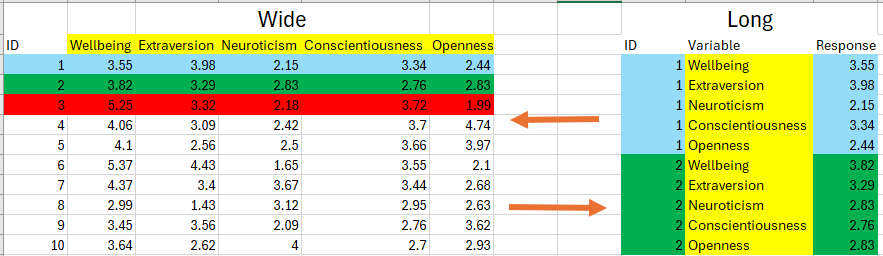
\includegraphics{img/06-pivot-visualisation.png}
\caption{\label{fig:unnamed-chunk-226}Visual representation of what is pivoted}
\end{figure}

\hypertarget{pivoting-our-remote-associations-data-frame}{%
\subsection{Pivoting our Remote Associations Data Frame}\label{pivoting-our-remote-associations-data-frame}}

Last week, we cleaned the \texttt{raw\_remote\_associations.csv} data frame to a variable called \texttt{df\_clean.} If we used \texttt{head()}, we'll see that it is in wide format

\begin{Shaded}
\begin{Highlighting}[]
\CommentTok{\#if you do not have df\_clean in your environment, download the dataset \textasciigrave{}raw\_remote\_clean.csv\textasciigrave{} from the Teams channel, and put in the week 5 folder. }

\CommentTok{\#Run the following code to load it in }
\CommentTok{\#df\_clean \textless{}{-} read.csv("raw\_remote\_clean.csv") }

\FunctionTok{head}\NormalTok{(df\_clean)}
\end{Highlighting}
\end{Shaded}

\begin{verbatim}
##         ID condition age gender remote_pos remote_neg remote_neut total_mood
## 1 10229436       CAB  26   male          0          2           4         61
## 2 10230533       CAB  36 female          0          4           4         62
## 3 10230659       ABC  45 female          0          5           0         74
## 4 10428518       BCA  37   male          0          9           9         68
## 5 10229522       CAB  30 female          1          1           0         59
## 6 10229414       ABC  36 female          1          1           1         63
##   total_openness mean_openness
## 1             16           3.2
## 2             15           3.0
## 3             17           3.4
## 4             14           2.8
## 5             16           3.2
## 6             14           2.8
\end{verbatim}

Let's convert \texttt{df\_clean} to the long data format and let's call it \texttt{df\_clean\_long}. But we are not going to follow the same protocol as the last example, where we pivoted everything except \texttt{ID}. For this data frame, we are going put every variable inside the \texttt{cols} argument except for \texttt{ID}, \texttt{condition}, and \texttt{gender}.

\begin{Shaded}
\begin{Highlighting}[]
\NormalTok{df\_clean\_long }\OtherTok{\textless{}{-}} \FunctionTok{pivot\_longer}\NormalTok{(df\_clean,}
  \AttributeTok{cols =} \FunctionTok{c}\NormalTok{(age, remote\_pos}\SpecialCharTok{:}\NormalTok{mean\_openness), }\CommentTok{\#we select age, and then we select everything from remote\_pos to mean\_openness in df\_clean}
  \AttributeTok{names\_to =} \StringTok{"Variable"}\NormalTok{, }\CommentTok{\#this creates a column called \textasciigrave{}variables\textasciigrave{} that will tell us the the variable the participant provided data for}
  \AttributeTok{values\_to =} \StringTok{"Response"}\CommentTok{\#this creates a column called \textasciigrave{}answer\textasciigrave{} that will tell us participants actual answer to each variable}
\NormalTok{)}


\FunctionTok{print}\NormalTok{(df\_clean\_long)}
\end{Highlighting}
\end{Shaded}

\begin{verbatim}
## # A tibble: 266 x 5
##          ID condition gender Variable       Response
##       <int> <chr>     <chr>  <chr>             <dbl>
##  1 10229436 CAB       male   age                26  
##  2 10229436 CAB       male   remote_pos          0  
##  3 10229436 CAB       male   remote_neg          2  
##  4 10229436 CAB       male   remote_neut         4  
##  5 10229436 CAB       male   total_mood         61  
##  6 10229436 CAB       male   total_openness     16  
##  7 10229436 CAB       male   mean_openness       3.2
##  8 10230533 CAB       female age                36  
##  9 10230533 CAB       female remote_pos          0  
## 10 10230533 CAB       female remote_neg          4  
## # i 256 more rows
\end{verbatim}

There we have it! Now our data is long-format. Each row contains a participant's individuals score on a particular variable. But this time, the participant's information on \texttt{condition} and \texttt{gender} also gets replicated for row created for that participant.

But why did we not include the variables \texttt{condition} and \texttt{gender} in our conversion? There is both a technical reason and an data analysis reason for why we did not do this. Let's address the boring technical reason first.

Technically, we actually can't create the \texttt{Answer} column by combining participants responses on variables like \texttt{condition} and \texttt{gender} with their answers on the other variables. This is because the data type for both \texttt{condition} and \texttt{gender} are \texttt{factors}, whereas the data type for every other variable is \texttt{numeric}. If you remember from our vector discussion (and remember everything that every column is just a lucky vector who found a home) we mentioned that vectors are lines of data where everything in the line is of the same data type. You can have character vectors, factor vectors, numerical vectors, logical vectors, integer vectors, but you cannot have a single vector with multiple data types.

So if we try \texttt{pivot\_longer} on our \texttt{df\_clean} data frame, including the \texttt{gender} and \texttt{condition} columns, we get the following error:

\begin{Shaded}
\begin{Highlighting}[]
\FunctionTok{pivot\_longer}\NormalTok{(df\_clean,}
  \AttributeTok{cols =} \FunctionTok{c}\NormalTok{(condition}\SpecialCharTok{:}\NormalTok{mean\_openness), }\CommentTok{\#we try to select everything except ID}
  \AttributeTok{names\_to =} \StringTok{"Variable"}\NormalTok{, }\CommentTok{\#this creates a column called \textasciigrave{}variables\textasciigrave{} that will tell us the the variable the participant provided data for}
  \AttributeTok{values\_to =} \StringTok{"Response"}\CommentTok{\#this creates a column called \textasciigrave{}answer\textasciigrave{} that will tell us participants actual answer to each variable}
\NormalTok{)}
\end{Highlighting}
\end{Shaded}

\begin{verbatim}
## Error in `pivot_longer()`:
## ! Can't combine `condition` <character> and `age` <integer>.
\end{verbatim}

If you're stubborn and you insist on pivoting everything, then you would need to convert all of our columns to the same data type. There is an argument in the \texttt{pivot\_longer()} function that enables us to do this and it is called \texttt{values\_transform}. The easiest solution would be to transform everything that will go in our \texttt{Answer} vector/column into a \texttt{character}.

\begin{Shaded}
\begin{Highlighting}[]
\FunctionTok{pivot\_longer}\NormalTok{(df\_clean,}
  \AttributeTok{cols =}\NormalTok{ condition}\SpecialCharTok{:}\NormalTok{mean\_openness, }
  \AttributeTok{names\_to =} \StringTok{"Variable"}\NormalTok{, }
  \AttributeTok{values\_to =} \StringTok{"Response"}\NormalTok{,}
  \AttributeTok{values\_transform =} \FunctionTok{list}\NormalTok{(}\AttributeTok{Response =}\NormalTok{ as.character)}
\NormalTok{  )}
\end{Highlighting}
\end{Shaded}

\begin{verbatim}
## # A tibble: 342 x 3
##          ID Variable       Response
##       <int> <chr>          <chr>   
##  1 10229436 condition      CAB     
##  2 10229436 age            26      
##  3 10229436 gender         male    
##  4 10229436 remote_pos     0       
##  5 10229436 remote_neg     2       
##  6 10229436 remote_neut    4       
##  7 10229436 total_mood     61      
##  8 10229436 total_openness 16      
##  9 10229436 mean_openness  3.2     
## 10 10230533 condition      CAB     
## # i 332 more rows
\end{verbatim}

That is an example of a long data frame, which looks neater on the eye than our earlier attempt. BUT - I really do not recommend this approach. Since everything inside \texttt{answer} is not a character, we actually can't conduct any quantitative analysis. So it defeats the purpose!

This leads me on to the analytical reason why we don't want to pivot our \texttt{condition} and \texttt{gender} columns. Since \texttt{condition} and \texttt{gender} are factors, we will want to investigate the extent to which participants scores on \texttt{Wellbeing} and our Big Five traits are influenced by differences in each factor. In other words, we want to investigate the effect of our independent variables on our dependent variables. If you look at \texttt{df\_clean\_long}, the data frame keeps a record of a participant's score on each dependent variable in relation to our two independent variables. This sets us up nicely for conducting statistical analysis.

\begin{verbatim}
## # A tibble: 10 x 5
##          ID condition gender Variable       Response
##       <int> <chr>     <chr>  <chr>             <dbl>
##  1 10229436 CAB       male   age                26  
##  2 10229436 CAB       male   remote_pos          0  
##  3 10229436 CAB       male   remote_neg          2  
##  4 10229436 CAB       male   remote_neut         4  
##  5 10229436 CAB       male   total_mood         61  
##  6 10229436 CAB       male   total_openness     16  
##  7 10229436 CAB       male   mean_openness       3.2
##  8 10230533 CAB       female age                36  
##  9 10230533 CAB       female remote_pos          0  
## 10 10230533 CAB       female remote_neg          4
\end{verbatim}

\hypertarget{pivoting-from-long-to-wide}{%
\subsection{Pivoting from Long to Wide}\label{pivoting-from-long-to-wide}}

Okay, so we know how to convert data frames from wide to long, but how can we convert from long to wide? Well we can use the \texttt{pivot\_wider()} function. The figure below shows the results of typing \texttt{?pivot\_wider} into the console. The table below it shows the key arguments of this function.

\begin{figure}
\centering
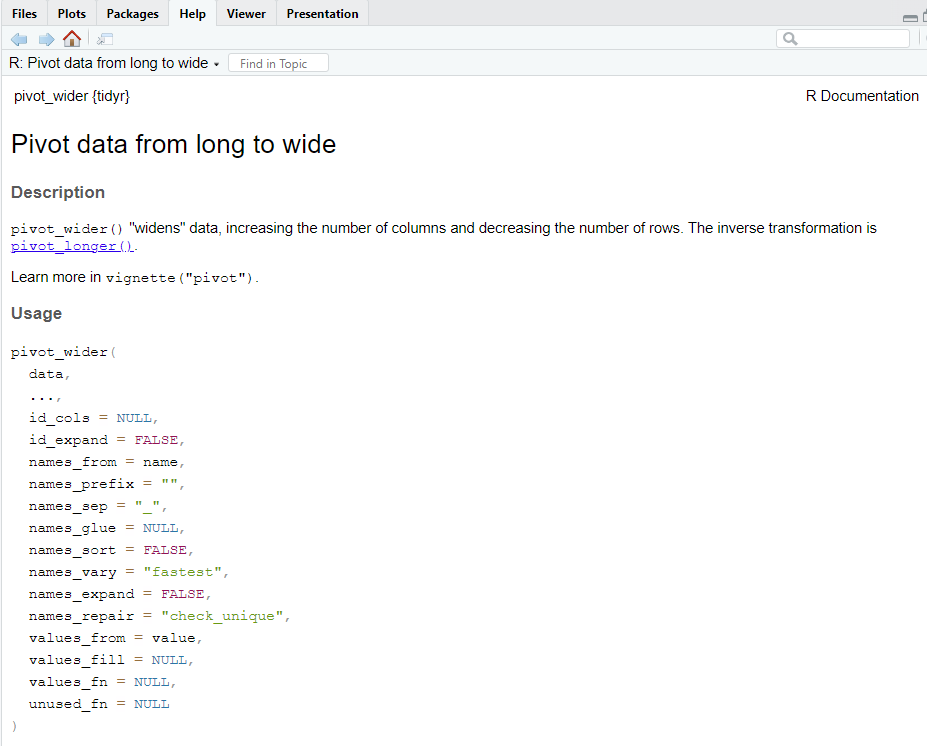
\includegraphics{img/06-pivotwider.png}
\caption{\label{fig:unnamed-chunk-232}The arguments that we can pass to the pivot\_wider() function}
\end{figure}

\begin{longtable}[]{@{}
  >{\raggedright\arraybackslash}p{(\columnwidth - 2\tabcolsep) * \real{0.2639}}
  >{\raggedright\arraybackslash}p{(\columnwidth - 2\tabcolsep) * \real{0.7361}}@{}}
\toprule\noalign{}
\begin{minipage}[b]{\linewidth}\raggedright
Argument
\end{minipage} & \begin{minipage}[b]{\linewidth}\raggedright
Meaning
\end{minipage} \\
\midrule\noalign{}
\endhead
\bottomrule\noalign{}
\endlastfoot
\texttt{data} & The long data frame that you want to convert to wide format \\
\texttt{id\_cols} & The columns that help identify each participant. This is often the values that are repeated in each row within a long data frame (e.g., like ID or any independent variables) \\
\texttt{names\_from} & When we pivot from long to wide, we will be creating new columns for each variable that we collected data on. We need to tell R where to find the names for those variables. \\
\texttt{values\_from} & We need to tell R where to find the values for the new columns that we are creating. \\
\end{longtable}

Let's convert our \texttt{long\_df} back into wide format.

\begin{Shaded}
\begin{Highlighting}[]
\FunctionTok{pivot\_wider}\NormalTok{(long\_df, }
            \AttributeTok{id\_cols =}\NormalTok{ ID, }
            \AttributeTok{names\_from =}\NormalTok{ Variable,}
            \AttributeTok{values\_from =}\NormalTok{ Response)}
\end{Highlighting}
\end{Shaded}

\begin{verbatim}
## # A tibble: 10 x 6
##       ID Wellbeing Extraversion Neuroticism Conscientiousness Openness
##    <int>     <dbl>        <dbl>       <dbl>             <dbl>    <dbl>
##  1     1      3.55         3.98        2.15              3.34     2.44
##  2     2      3.82         3.29        2.83              2.76     2.83
##  3     3      5.25         3.32        2.18              3.72     1.99
##  4     4      4.06         3.09        2.42              3.7      4.74
##  5     5      4.1          2.56        2.5               3.66     3.97
##  6     6      5.37         4.43        1.65              3.55     2.1 
##  7     7      4.37         3.4         3.67              3.44     2.68
##  8     8      2.99         1.43        3.12              2.95     2.63
##  9     9      3.45         3.56        2.09              2.76     3.62
## 10    10      3.64         2.62        4                 2.7      2.93
\end{verbatim}

Look familiar? If you compare it to our original \texttt{wide\_df}, you'll notice they look exactly the same.

Now let's do the same thing with the long version of \texttt{remote\_associations} data frame.

\begin{Shaded}
\begin{Highlighting}[]
\NormalTok{df\_clean\_wide }\OtherTok{\textless{}{-}} \FunctionTok{pivot\_wider}\NormalTok{(df\_clean\_long,}
                             \AttributeTok{id\_cols =}\NormalTok{ ID}\SpecialCharTok{:}\NormalTok{gender,}
                             \AttributeTok{names\_from =}\NormalTok{ Variable,}
                             \AttributeTok{values\_from =}\NormalTok{ Response)}

\FunctionTok{head}\NormalTok{(df\_clean\_wide)}
\end{Highlighting}
\end{Shaded}

\begin{verbatim}
## # A tibble: 6 x 10
##         ID condition gender   age remote_pos remote_neg remote_neut total_mood
##      <int> <chr>     <chr>  <dbl>      <dbl>      <dbl>       <dbl>      <dbl>
## 1 10229436 CAB       male      26          0          2           4         61
## 2 10230533 CAB       female    36          0          4           4         62
## 3 10230659 ABC       female    45          0          5           0         74
## 4 10428518 BCA       male      37          0          9           9         68
## 5 10229522 CAB       female    30          1          1           0         59
## 6 10229414 ABC       female    36          1          1           1         63
## # i 2 more variables: total_openness <dbl>, mean_openness <dbl>
\end{verbatim}

If you compare that to the head of \texttt{df\_clean}, you'll see that its back to the format we cleaned it to last week.

\hypertarget{summary-6}{%
\subsubsection{Summary}\label{summary-6}}

That covers basic pivoting from long to wide and wide to long using \texttt{pivot\_long()} and \texttt{pivot\_wide()}. However, both functions enable you to handle much more complicated data frames and clean them up as you go. We won't cover that in this version of the textbook, but \href{https://dcl-wrangle.stanford.edu/pivot-advanced.html}{I highly recommend reading the \texttt{Advanced\ Pivoting} section from the \texttt{Data\ Wrangling} Standford ebook if your pivoting needs are more complicated than the examples here}.

\hypertarget{handling-missing-values}{%
\section{Handling Missing Values}\label{handling-missing-values}}

In psychological research, dealing with missing data is a common challenge that requires careful consideration to ensure the integrity and validity of analyses. In this section, we'll explore how to handle missing values (NA) in R using the tidyverse package. We'll cover techniques for identifying missing values, strategies for handling them, and best practices for addressing missing data in psychological research studies.

\hypertarget{introduction-to-missing-values}{%
\subsection{\texorpdfstring{\textbf{Introduction to Missing Values}}{Introduction to Missing Values}}\label{introduction-to-missing-values}}

Missing values, often represented as NA in R, occur when data is not available or cannot be recorded for certain observations. This can occur due to various reasons such as non-response in surveys, data entry errors, or incomplete data collection processes. It's essential to understand and address missing values appropriately to avoid biased or misleading results in data analysis.

\hypertarget{identifying-missing-values}{%
\subsection{\texorpdfstring{\textbf{Identifying Missing Values}}{Identifying Missing Values}}\label{identifying-missing-values}}

Detecting missing values in datasets is the first step towards handling them effectively. In R, we can use functions like \textbf{\texttt{is.na()}} or \textbf{\texttt{complete.cases()}} to identify missing values. Let's illustrate this with an example using a hypothetical psychological research dataset:

\begin{Shaded}
\begin{Highlighting}[]
\CommentTok{\# Example dataset with missing values}
\NormalTok{data }\OtherTok{\textless{}{-}} \FunctionTok{tibble}\NormalTok{(}
  \AttributeTok{id =} \DecValTok{1}\SpecialCharTok{:}\DecValTok{10}\NormalTok{,}
  \AttributeTok{age =} \FunctionTok{c}\NormalTok{(}\DecValTok{25}\NormalTok{, }\ConstantTok{NA}\NormalTok{, }\DecValTok{30}\NormalTok{, }\DecValTok{28}\NormalTok{, }\DecValTok{35}\NormalTok{, }\ConstantTok{NA}\NormalTok{, }\DecValTok{40}\NormalTok{, }\DecValTok{22}\NormalTok{, }\ConstantTok{NA}\NormalTok{, }\DecValTok{29}\NormalTok{),}
  \AttributeTok{gender =} \FunctionTok{c}\NormalTok{(}\StringTok{"Male"}\NormalTok{, }\StringTok{"Female"}\NormalTok{, }\StringTok{"Male"}\NormalTok{, }\ConstantTok{NA}\NormalTok{, }\StringTok{"Female"}\NormalTok{, }\StringTok{"Male"}\NormalTok{, }\ConstantTok{NA}\NormalTok{, }\StringTok{"Male"}\NormalTok{, }\StringTok{"Female"}\NormalTok{, }\ConstantTok{NA}\NormalTok{)}
\NormalTok{)}

\CommentTok{\# Check for missing values}
\NormalTok{missing\_values }\OtherTok{\textless{}{-}}\NormalTok{ data }\SpecialCharTok{\%\textgreater{}\%}
  \FunctionTok{summarise\_all}\NormalTok{(}\SpecialCharTok{\textasciitilde{}}\FunctionTok{sum}\NormalTok{(}\FunctionTok{is.na}\NormalTok{(.)))}

\FunctionTok{print}\NormalTok{(missing\_values)}
\end{Highlighting}
\end{Shaded}

\begin{verbatim}
## # A tibble: 1 x 3
##      id   age gender
##   <int> <int>  <int>
## 1     0     3      3
\end{verbatim}

In this example, we've created a dataset \textbf{\texttt{data}} with variables \textbf{\texttt{age}} and \textbf{\texttt{gender}}, some of which contain missing values. We then used \textbf{\texttt{summarise\_all()}} along with \textbf{\texttt{is.na()}} to count the number of missing values in each column.

\hypertarget{dealing-with-missing-values}{%
\subsection{\texorpdfstring{\textbf{Dealing with Missing Values}}{Dealing with Missing Values}}\label{dealing-with-missing-values}}

Once missing values are identified, we can employ various strategies to handle them effectively. Common approaches include removing rows or columns with missing values, imputing missing values with estimates, or using more advanced imputation methods.

\hypertarget{removing-missing-values}{%
\subsubsection{Removing Missing Values}\label{removing-missing-values}}

To remove rows or columns with missing values, we can use functions like \textbf{\texttt{drop\_na()}} or \textbf{\texttt{filter()}} in the tidyverse. Here's how we can remove rows with missing values in the \textbf{\texttt{age}} column:

\begin{Shaded}
\begin{Highlighting}[]
\CommentTok{\# Remove rows with missing values in the age column}
\NormalTok{clean\_data }\OtherTok{\textless{}{-}}\NormalTok{ data }\SpecialCharTok{\%\textgreater{}\%}
  \FunctionTok{drop\_na}\NormalTok{(age)}

\FunctionTok{print}\NormalTok{(clean\_data)}
\end{Highlighting}
\end{Shaded}

\begin{verbatim}
## # A tibble: 7 x 3
##      id   age gender
##   <int> <dbl> <chr> 
## 1     1    25 Male  
## 2     3    30 Male  
## 3     4    28 <NA>  
## 4     5    35 Female
## 5     7    40 <NA>  
## 6     8    22 Male  
## 7    10    29 <NA>
\end{verbatim}

\begin{Shaded}
\begin{Highlighting}[]
\CommentTok{\#filter}
\end{Highlighting}
\end{Shaded}

\hypertarget{imputing-missing-values}{%
\subsubsection{Imputing Missing Values}\label{imputing-missing-values}}

Imputing missing values involves replacing them with estimates such as mean, median, or mode. Let's impute missing values in the \textbf{\texttt{age}} column with the mean age:

\begin{Shaded}
\begin{Highlighting}[]
\CommentTok{\# Impute missing values in the age column with mean age}
\NormalTok{imputed\_data }\OtherTok{\textless{}{-}}\NormalTok{ data }\SpecialCharTok{\%\textgreater{}\%}
  \FunctionTok{mutate}\NormalTok{(}\AttributeTok{age =} \FunctionTok{if\_else}\NormalTok{(}\FunctionTok{is.na}\NormalTok{(age), }\FunctionTok{mean}\NormalTok{(age, }\AttributeTok{na.rm =} \ConstantTok{TRUE}\NormalTok{), age))}

\FunctionTok{print}\NormalTok{(imputed\_data)}
\end{Highlighting}
\end{Shaded}

\begin{verbatim}
## # A tibble: 10 x 3
##       id   age gender
##    <int> <dbl> <chr> 
##  1     1  25   Male  
##  2     2  29.9 Female
##  3     3  30   Male  
##  4     4  28   <NA>  
##  5     5  35   Female
##  6     6  29.9 Male  
##  7     7  40   <NA>  
##  8     8  22   Male  
##  9     9  29.9 Female
## 10    10  29   <NA>
\end{verbatim}

\hypertarget{best-practices-and-considerations}{%
\subsection{\texorpdfstring{\textbf{Best Practices and Considerations}}{Best Practices and Considerations}}\label{best-practices-and-considerations}}

When handling missing values, it's important to adhere to best practices and consider the following:

\begin{itemize}
\item
  Document the handling of missing values in data preprocessing steps.
\item
  Conduct sensitivity analyses to assess the robustness of results to different missing data handling approaches.
\item
  Consider potential biases introduced by missing data and address them in the interpretation of results.
\end{itemize}

\hypertarget{summary-7}{%
\subsection{\texorpdfstring{\textbf{Summary}}{Summary}}\label{summary-7}}

Handling missing values is a critical aspect of data preprocessing in psychological research. By using the tidyverse package in R, researchers can effectively identify and handle missing values, ensuring the integrity and validity of their data analysis. In this section, we've covered techniques for identifying missing values, strategies for handling them, and best practices for addressing missing data. Through practical examples and considerations, researchers can confidently manage missing values in their research studies.

\hypertarget{merging-data-i.e.-joining-different-datasets-together}{%
\section{Merging Data (i.e., Joining Different Datasets Together)}\label{merging-data-i.e.-joining-different-datasets-together}}

In psychological research, we'll often encounter situations where data from multiple sources or studies need to be combined for analysis. We might have collected demographic information separately from participants answers on experimental tasks. We may have collected data using a variety of platforms (e.g., survey data using Qualtrics and response data using PsychoPy). Additionally, the research software tools we use might modulate the data. For example, if we run a study in Gorilla Research, then each separate task and questionnaire gets downloaded as separate files.

Whatever the reason, you will often need to merge or join data together from different sources in order to conduct the analysis you need. Luckily, R is quite capable at facilitating data merging. In this subsection, we will look at ways you can merge different data frames together.

\hypertarget{introduction-to-merging-data}{%
\subsection{Introduction to Merging Data}\label{introduction-to-merging-data}}

Merging data involves combining data frames based on their common variables. Let's image we have two data frames called \texttt{df\_demographics} and \texttt{df\_rt}. These data frames contain information on both participants demographic information and their reaction time on a specific task and which condition they were randomly assigned to. Let's load both of these data frames into R (make sure you have downloaded them and put them into your working directory before running the following code).

\begin{Shaded}
\begin{Highlighting}[]
\NormalTok{df\_demographics }\OtherTok{\textless{}{-}} \FunctionTok{read.csv}\NormalTok{(}\StringTok{"demographics.csv"}\NormalTok{)}
\NormalTok{df\_rt }\OtherTok{\textless{}{-}} \FunctionTok{read.csv}\NormalTok{(}\StringTok{"reaction\_time.csv"}\NormalTok{)}

\FunctionTok{head}\NormalTok{(df\_demographics)}
\FunctionTok{head}\NormalTok{(df\_rt)}
\end{Highlighting}
\end{Shaded}

\begin{verbatim}
##           ID     gender age
## 1 EoYncPX1QK     Female  24
## 2 Zn1yzAeYA4 Non-Binary  21
## 3 B4iCIhzgPi       Male  24
## 4 9sJnqQM0lo     Female  23
## 5 FPSgiOjwA7 Non-Binary  23
## 6 0g0AFLyHCe       Male  24
\end{verbatim}

\begin{verbatim}
##           ID   condition mean_rt
## 1 EoYncPX1QK no caffeine     269
## 2 Zn1yzAeYA4 no caffeine     206
## 3 B4iCIhzgPi no caffeine     187
## 4 9sJnqQM0lo no caffeine     217
## 5 FPSgiOjwA7 no caffeine     160
## 6 0g0AFLyHCe no caffeine     255
\end{verbatim}

Ideally, we would have one merged data frame that would contain a participant's response on all our variables. However, there are some complications with these two data frames. If you check the number of rows in each data frame, we can see there are differing number of participants.

\begin{Shaded}
\begin{Highlighting}[]
\FunctionTok{nrow}\NormalTok{(df\_demographics)}
\end{Highlighting}
\end{Shaded}

\begin{verbatim}
## [1] 60
\end{verbatim}

\begin{Shaded}
\begin{Highlighting}[]
\FunctionTok{nrow}\NormalTok{(df\_rt)}
\end{Highlighting}
\end{Shaded}

\begin{verbatim}
## [1] 42
\end{verbatim}

There are 60 participants in the demographics data frame whereas there are only 42 participants in the reaction time data frame. If the study was online, maybe participants gave up after completing the demographic information, maybe there was connection issues, maybe the data did not save correctly. Whatever the reason for this mismatch in participants, we need to account for this when we merge these data frames together.

Luckily, there are a multitude in ways we can do this through the \texttt{tidyverse\ package}.

These types of join are:

\begin{itemize}
\item
  \textbf{Inner Join}: Includes only the rows that have matching values in both datasets. This type of join retains only the observations that exist in both datasets, excluding unmatched rows.
\item
  \textbf{Left Join}: Includes all rows from the left dataset and matching rows from the right dataset. Unmatched rows from the right dataset are filled with NA values.
\item
  \textbf{Right Join}: Includes all rows from the right dataset and matching rows from the left dataset. Unmatched rows from the left dataset are filled with NA values.
\item
  \textbf{Outer Join (or Full Join)}: Includes all rows from both datasets, filling in missing values with NA where there are no matches.
\end{itemize}

Using our \texttt{df\_demographics} and \texttt{df\_rt} data frames, lets show you the result of each of these joins and why/when you would use them.

\hypertarget{inner_join}{%
\subsection{Inner\_Join}\label{inner_join}}

The \texttt{inner\_join()} function joins together two data frames, but it will only keep the rows that have matching values in both data frames.

When we use \texttt{inner\_join()} we need to specify the value(s) that we want to match across both data frames. Once we do, then in the case of the \texttt{df\_demographics} and \texttt{df\_rt} data frames, what this means is that only the participants who match on that specified value(s) in both data frames will merged together.

Let's create a merged data frame using \texttt{inner\_join} and call it \texttt{df\_inner}. The syntax for inner\_join is: \texttt{inner\_join(df1,\ df2,\ by\ =\ join\_by(column(s))}

\begin{Shaded}
\begin{Highlighting}[]
\NormalTok{df\_inner }\OtherTok{\textless{}{-}} \FunctionTok{inner\_join}\NormalTok{(df\_demographics, df\_rt, }\AttributeTok{by =} \StringTok{"ID"}\NormalTok{)}

\FunctionTok{head}\NormalTok{(df\_inner)}
\end{Highlighting}
\end{Shaded}

\begin{verbatim}
##           ID     gender age   condition mean_rt
## 1 EoYncPX1QK     Female  24 no caffeine     269
## 2 Zn1yzAeYA4 Non-Binary  21 no caffeine     206
## 3 B4iCIhzgPi       Male  24 no caffeine     187
## 4 9sJnqQM0lo     Female  23 no caffeine     217
## 5 FPSgiOjwA7 Non-Binary  23 no caffeine     160
## 6 0g0AFLyHCe       Male  24 no caffeine     255
\end{verbatim}

We can see that our \texttt{df\_inner} has combined the \texttt{gender} and \texttt{age} columns from \texttt{df\_demographics} with the \texttt{condition} and \texttt{mean\_rt} columns from \texttt{df\_rt}. When we use \texttt{inner\_join} the order in which specify the data frames is the order in which the columns will be added. So if we wanted the \texttt{condition} and \texttt{mean\_rt} columns to come first, then we can change the order:

\begin{Shaded}
\begin{Highlighting}[]
\FunctionTok{inner\_join}\NormalTok{(df\_rt, df\_demographics, }\AttributeTok{by =} \FunctionTok{join\_by}\NormalTok{(ID))}
\end{Highlighting}
\end{Shaded}

\begin{verbatim}
##            ID     condition mean_rt     gender age
## 1  EoYncPX1QK   no caffeine     269     Female  24
## 2  Zn1yzAeYA4   no caffeine     206 Non-Binary  21
## 3  B4iCIhzgPi   no caffeine     187       Male  24
## 4  9sJnqQM0lo   no caffeine     217     Female  23
## 5  FPSgiOjwA7   no caffeine     160 Non-Binary  23
## 6  0g0AFLyHCe   no caffeine     255       Male  24
## 7  hlmrG4AyLu   no caffeine     145     Female  22
## 8  oOUz7EpZDf   no caffeine     240 Non-Binary  24
## 9  QhvvMEVq1X   no caffeine     212       Male  24
## 10 WHdme1YyZv   no caffeine     207     Female  22
## 11 yFTywINVDl   no caffeine     236 Non-Binary  24
## 12 E4TDInCFgc   no caffeine     157       Male  23
## 13 w15ouKhYjX   no caffeine     139     Female  24
## 14 PRHjvltTq9   no caffeine     185 Non-Binary  23
## 15 T1INTYDoxW  low caffeine     261       Male  23
## 16 wQgCowzLTF  low caffeine     229     Female  22
## 17 gAPefpxFu2  low caffeine     314 Non-Binary  23
## 18 kJRT78syM1  low caffeine     150       Male  24
## 19 zigHVms3ZU  low caffeine     205     Female  23
## 20 MdaNDDZypx  low caffeine     353 Non-Binary  24
## 21 1kVtNcCJZR  low caffeine     201       Male  21
## 22 vWP6tk42hT  low caffeine     245     Female  23
## 23 uSbQmTf4hR  low caffeine     242 Non-Binary  24
## 24 F5JS8n0pw8  low caffeine     281       Male  24
## 25 GNNjyhr80i  low caffeine     203     Female  22
## 26 gg587jx1wz  low caffeine     260 Non-Binary  22
## 27 QG48CYj01m  low caffeine     113       Male  22
## 28 QkyZzgywzF  low caffeine     162     Female  23
## 29 t8x4iOKwnT high caffeine     204 Non-Binary  22
## 30 fAazPW5qCz high caffeine     170       Male  23
## 31 Aug70zOtfX high caffeine     211     Female  22
## 32 DECqK4tIyT high caffeine     114 Non-Binary  23
## 33 GbdjGe0yh2 high caffeine     227       Male  24
## 34 yuSrPEfg8O high caffeine     175     Female  24
## 35 Vq0SB0N0gt high caffeine     177 Non-Binary  23
## 36 rCqGbWbmxW high caffeine     192       Male  22
## 37 crbKl4mP8f high caffeine     171     Female  22
## 38 PPL7VpIJAA high caffeine     114 Non-Binary  23
## 39 I8wcEVbUwc high caffeine     230       Male  22
## 40 i8MDEDiJHv high caffeine     201     Female  23
## 41 5ROBC8QMSK high caffeine      48 Non-Binary  22
## 42 QGslHuqlDI high caffeine     255       Male  23
\end{verbatim}

If we check the number of rows, we will see that it matches the number of rows in \texttt{df\_rt} rather than \texttt{df\_demographics}.

\begin{Shaded}
\begin{Highlighting}[]
\FunctionTok{nrow}\NormalTok{(df\_inner)}
\end{Highlighting}
\end{Shaded}

\begin{verbatim}
## [1] 42
\end{verbatim}

\hypertarget{left_join}{%
\subsection{Left\_join}\label{left_join}}

The function \texttt{left\_join} keeps every participant (row) in the first data frame we feed it. It then matches participants responses in the second data frame and joins them together, once we specify a value that needs to be matched. If there is not a match on that column, then it fills the results with \texttt{NA} values.

Let's create the data frame \texttt{df\_left} using \texttt{left\_join()}. The syntax for this function is: \texttt{left\_join(df1,\ df2,\ by\ =\ join\_by(ID))}.

\begin{Shaded}
\begin{Highlighting}[]
\NormalTok{df\_left }\OtherTok{\textless{}{-}} \FunctionTok{left\_join}\NormalTok{(df\_demographics, df\_rt, }\AttributeTok{by =} \FunctionTok{join\_by}\NormalTok{(ID))}


\FunctionTok{head}\NormalTok{(df\_left)}
\end{Highlighting}
\end{Shaded}

\begin{verbatim}
##           ID     gender age   condition mean_rt
## 1 EoYncPX1QK     Female  24 no caffeine     269
## 2 Zn1yzAeYA4 Non-Binary  21 no caffeine     206
## 3 B4iCIhzgPi       Male  24 no caffeine     187
## 4 9sJnqQM0lo     Female  23 no caffeine     217
## 5 FPSgiOjwA7 Non-Binary  23 no caffeine     160
## 6 0g0AFLyHCe       Male  24 no caffeine     255
\end{verbatim}

\begin{Shaded}
\begin{Highlighting}[]
\FunctionTok{tail}\NormalTok{(df\_left) }\CommentTok{\#prints out the last six rows of a data frame}
\end{Highlighting}
\end{Shaded}

\begin{verbatim}
##            ID     gender age condition mean_rt
## 55 TNfJ2PV63D     Female  24      <NA>      NA
## 56 VZjyLYJOyd Non-Binary  23      <NA>      NA
## 57 oZv0WxMU7K       Male  21      <NA>      NA
## 58 T1UopshE5K     Female  24      <NA>      NA
## 59 MZV79pikQY Non-Binary  24      <NA>      NA
## 60 D8j28H49Lt       Male  23      <NA>      NA
\end{verbatim}

\begin{Shaded}
\begin{Highlighting}[]
\FunctionTok{nrow}\NormalTok{(df\_left)}
\end{Highlighting}
\end{Shaded}

\begin{verbatim}
## [1] 60
\end{verbatim}

We can see that every participant in the \texttt{df\_demographics} is included inside the \texttt{df\_left} data frame. If that participant does not have scores on \texttt{condition} and \texttt{mean\_rt}, then \texttt{NA} is substituted in.

The function is called \texttt{left\_join()} because it joins whatever is put first (i.e., left) in the function is given priority over what comes second (i.e., right). The next merging function we'll discuss does the opposite.

\hypertarget{right_join}{%
\subsection{Right\_Join}\label{right_join}}

The function \texttt{left\_join} keeps every participant (row) in the second data frame we feed it. It then matches participants responses in the first data frame and joins them together, once we specify a value that needs to be matched. If there is not a match on that column, then it fills the results with \texttt{NA} values.

Let's create the data frame \texttt{df\_left} using \texttt{left\_join()}. The syntax for this function is: \texttt{right\_join(df1,\ df2,\ by\ =\ join\_by(ID))}

\begin{Shaded}
\begin{Highlighting}[]
\NormalTok{df\_right }\OtherTok{\textless{}{-}} \FunctionTok{right\_join}\NormalTok{(df\_demographics, df\_rt, }\AttributeTok{by =} \FunctionTok{join\_by}\NormalTok{(ID))}

\FunctionTok{head}\NormalTok{(df\_right)}
\end{Highlighting}
\end{Shaded}

\begin{verbatim}
##           ID     gender age   condition mean_rt
## 1 EoYncPX1QK     Female  24 no caffeine     269
## 2 Zn1yzAeYA4 Non-Binary  21 no caffeine     206
## 3 B4iCIhzgPi       Male  24 no caffeine     187
## 4 9sJnqQM0lo     Female  23 no caffeine     217
## 5 FPSgiOjwA7 Non-Binary  23 no caffeine     160
## 6 0g0AFLyHCe       Male  24 no caffeine     255
\end{verbatim}

\begin{Shaded}
\begin{Highlighting}[]
\FunctionTok{tail}\NormalTok{(df\_right)}
\end{Highlighting}
\end{Shaded}

\begin{verbatim}
##            ID     gender age     condition mean_rt
## 37 crbKl4mP8f     Female  22 high caffeine     171
## 38 PPL7VpIJAA Non-Binary  23 high caffeine     114
## 39 I8wcEVbUwc       Male  22 high caffeine     230
## 40 i8MDEDiJHv     Female  23 high caffeine     201
## 41 5ROBC8QMSK Non-Binary  22 high caffeine      48
## 42 QGslHuqlDI       Male  23 high caffeine     255
\end{verbatim}

\begin{Shaded}
\begin{Highlighting}[]
\FunctionTok{nrow}\NormalTok{(df\_right)}
\end{Highlighting}
\end{Shaded}

\begin{verbatim}
## [1] 42
\end{verbatim}

In this case, because every participant ID in \texttt{df\_rt} has a matching response in \texttt{df\_demographics}, we do not see any \texttt{NA} values.

You might be wondering why the hell would you want both a \texttt{left\_join()} and a \texttt{right\_join()} function. Couldn't we have just the one function, and just specify which order we want to join things together?

We could, but having the option of having \texttt{left\_join()} and \texttt{right\_join()} becomes handy when we have complicated and deeply nested code using the pipe \texttt{\%\textgreater{}\%} operator.

But nonetheless you may never have a need for both functions, but in case you do, you know it's there.

\hypertarget{outer-join}{%
\subsection{Outer Join}\label{outer-join}}

The \textbf{outer join}, also known as a \textbf{full join}, combines rows from both datasets, including all observations from both data frames and filling in missing values with NA where there are no matches. This type of join ensures that no data is lost, even if there are unmatched rows in either dataset.

Let's demonstrate the outer join using two new data frames: \textbf{\texttt{df\_scores}} and \textbf{\texttt{df\_survey}}. These data frames contain information on participants' test scores and survey responses, respectively. The \textbf{\texttt{df\_scores}} data frame will have scores for participants 1-5, whereas the \textbf{\texttt{df\_survey}} data frame will have scores for participants 3-7. So there will be some overlap in data, but also some areas where there is not matching scores.

\begin{Shaded}
\begin{Highlighting}[]
\CommentTok{\# Creating sample data frames}
\NormalTok{df\_scores }\OtherTok{\textless{}{-}} \FunctionTok{data.frame}\NormalTok{(}
  \AttributeTok{ID =} \FunctionTok{c}\NormalTok{(}\DecValTok{1}\NormalTok{, }\DecValTok{2}\NormalTok{, }\DecValTok{3}\NormalTok{, }\DecValTok{4}\NormalTok{, }\DecValTok{5}\NormalTok{),}
  \AttributeTok{Test\_Score =} \FunctionTok{c}\NormalTok{(}\DecValTok{85}\NormalTok{, }\DecValTok{92}\NormalTok{, }\DecValTok{78}\NormalTok{, }\DecValTok{90}\NormalTok{, }\DecValTok{88}\NormalTok{)}
\NormalTok{)}

\NormalTok{df\_survey }\OtherTok{\textless{}{-}} \FunctionTok{data.frame}\NormalTok{(}
  \AttributeTok{ID =} \FunctionTok{c}\NormalTok{(}\DecValTok{3}\NormalTok{, }\DecValTok{4}\NormalTok{, }\DecValTok{5}\NormalTok{, }\DecValTok{6}\NormalTok{, }\DecValTok{7}\NormalTok{),}
  \AttributeTok{Satisfaction =} \FunctionTok{c}\NormalTok{(}\StringTok{"High"}\NormalTok{, }\StringTok{"Medium"}\NormalTok{, }\StringTok{"Low"}\NormalTok{, }\StringTok{"High"}\NormalTok{, }\StringTok{"Medium"}\NormalTok{)}
\NormalTok{)}

\CommentTok{\# Displaying the sample data frames}
\FunctionTok{head}\NormalTok{(df\_scores)}
\end{Highlighting}
\end{Shaded}

\begin{verbatim}
##   ID Test_Score
## 1  1         85
## 2  2         92
## 3  3         78
## 4  4         90
## 5  5         88
\end{verbatim}

\begin{Shaded}
\begin{Highlighting}[]
\FunctionTok{head}\NormalTok{(df\_survey)}
\end{Highlighting}
\end{Shaded}

\begin{verbatim}
##   ID Satisfaction
## 1  3         High
## 2  4       Medium
## 3  5          Low
## 4  6         High
## 5  7       Medium
\end{verbatim}

Now, let's join them together. The syntax for \textbf{\texttt{full\_join()}} is: \textbf{\texttt{full\_join(df1,\ df2,\ by\ =\ join\_by(column))}}

\begin{Shaded}
\begin{Highlighting}[]
\CommentTok{\# Performing outer join}
\NormalTok{df\_outer }\OtherTok{\textless{}{-}} \FunctionTok{full\_join}\NormalTok{(df\_scores, df\_survey, }\AttributeTok{by =} \StringTok{"ID"}\NormalTok{)}


\NormalTok{df\_outer}
\end{Highlighting}
\end{Shaded}

\begin{verbatim}
##   ID Test_Score Satisfaction
## 1  1         85         <NA>
## 2  2         92         <NA>
## 3  3         78         High
## 4  4         90       Medium
## 5  5         88          Low
## 6  6         NA         High
## 7  7         NA       Medium
\end{verbatim}

In the resulting \textbf{\texttt{df\_outer}} data frame, all rows from both \textbf{\texttt{df\_scores}} and \textbf{\texttt{df\_survey}} are included, regardless of whether there was a match on the specified column (\textbf{\texttt{ID}}). Rows with no matching values are filled with NA.

The outer join is particularly useful when you want to retain all information from both datasets, even if there are inconsistencies or missing values between them. This ensures that you have a complete dataset for analysis, with all available information from each source preserved.

\hypertarget{summary-8}{%
\subsection{Summary}\label{summary-8}}

Your choice of join ultimately depends on your research questions, the nature of your data, and the analysis you intend to perform. But hopefully at this point you have an appreciation of the variety of ways you can merge data in R.

\hypertarget{dealing-with-tricky-character-data}{%
\section{Dealing with Tricky Character Data}\label{dealing-with-tricky-character-data}}

\hypertarget{appendix---understanding-boolean-operators-in-the-context-of-filter}{%
\chapter{\texorpdfstring{Appendix - Understanding Boolean Operators in the Context of \texttt{filter()}}{Appendix - Understanding Boolean Operators in the Context of filter()}}\label{appendix---understanding-boolean-operators-in-the-context-of-filter}}

In the Chapter 5, I brushed over what the operators \texttt{\textless{}} and \texttt{\&}, and \texttt{\textbar{}} meant and what they were actually doing in R. Each of these operators are known as Boolean operators in R.

Boolean operators are logical operators used in programming to combine or modify conditions, resulting in either \textbf{\texttt{TRUE}} or \textbf{\texttt{FALSE}} outcomes. In the context of data cleaning in R, Boolean operators help us construct conditions to select specific rows from a data frame based on certain criteria. When using \textbf{\texttt{filter()}}, R evaluates each row in the data frame against the specified conditions, determining whether each row meets the criteria and should be retained or not.

\hypertarget{how-boolean-operators-work}{%
\section{How Boolean Operators Work:}\label{how-boolean-operators-work}}

\begin{itemize}
\item
  \textbf{Logical AND (\texttt{\&}):} The \textbf{\texttt{\&}} operator evaluates to \textbf{\texttt{TRUE}} only if both conditions on either side of the operator are \textbf{\texttt{TRUE}}. In the context of \textbf{\texttt{filter()}}, rows are retained if they satisfy \textbf{all} conditions joined by \textbf{\texttt{\&}}. For example, \textbf{\texttt{filter(df,\ x\ \textgreater{}\ 5\ \&\ y\ \textless{}\ 10)}} will retain rows where \textbf{\texttt{x}} is greater than \textbf{\texttt{5}} \textbf{and} \textbf{\texttt{y}} is less than \textbf{\texttt{10}}.
\item
  \textbf{Logical OR (\texttt{\textbar{}}):} The \textbf{\texttt{\textbar{}}} operator evaluates to \textbf{\texttt{TRUE}} if \textbf{at least one} of the conditions on either side of the operator is \textbf{\texttt{TRUE}}. In the context of \textbf{\texttt{filter()}}, rows are retained if they satisfy \textbf{any} of the conditions joined by \textbf{\texttt{\textbar{}}}. For example, \textbf{\texttt{filter(df,\ x\ \textgreater{}\ 5\ \textbar{}\ y\ \textless{}\ 10)}} will retain rows where \textbf{\texttt{x}} is greater than \textbf{\texttt{5}} \textbf{or} \textbf{\texttt{y}} is less than \textbf{\texttt{10}}.
\item
  \textbf{Logical NOT (\texttt{!}):} The \textbf{\texttt{!}} operator negates a condition, converting \textbf{\texttt{TRUE}} to \textbf{\texttt{FALSE}} and vice versa. In the context of \textbf{\texttt{filter()}}, \textbf{\texttt{!}} can be used to exclude rows that satisfy a particular condition. For example, \textbf{\texttt{filter(df,\ !(x\ ==\ 5))}} will exclude rows where \textbf{\texttt{x}} equals \textbf{\texttt{5}}.
\end{itemize}

\hypertarget{understanding-rs-evaluation-process}{%
\subsection{Understanding R's Evaluation Process:}\label{understanding-rs-evaluation-process}}

When applying \textbf{\texttt{filter()}} with Boolean operators, R sequentially evaluates each row in the data frame against the specified conditions. If a row satisfies \textbf{all} conditions joined by \textbf{\texttt{\&}}, or \textbf{any} condition joined by \textbf{\texttt{\textbar{}}}, it is retained in the filtered data frame. Rows that do not meet the specified criteria are excluded from the output.

The following table summarises the main Boolean operators we would use in R

\begin{longtable}[]{@{}
  >{\raggedright\arraybackslash}p{(\columnwidth - 4\tabcolsep) * \real{0.2192}}
  >{\raggedright\arraybackslash}p{(\columnwidth - 4\tabcolsep) * \real{0.5616}}
  >{\raggedright\arraybackslash}p{(\columnwidth - 4\tabcolsep) * \real{0.2192}}@{}}
\toprule\noalign{}
\begin{minipage}[b]{\linewidth}\raggedright
Operator/Condition
\end{minipage} & \begin{minipage}[b]{\linewidth}\raggedright
Description
\end{minipage} & \begin{minipage}[b]{\linewidth}\raggedright
Example
\end{minipage} \\
\midrule\noalign{}
\endhead
\bottomrule\noalign{}
\endlastfoot
\texttt{==} & Checks if two values are equal. & \texttt{x\ ==\ 5} evaluates to \texttt{TRUE} if \texttt{x} equals \texttt{5}. \\
\texttt{!=} & Checks if two values are not equal. & \texttt{x\ !=\ 5} evaluates to \texttt{TRUE} if \texttt{x} does not equal \texttt{5}. \\
\texttt{\textgreater{}} & Checks if one value is greater than another. & \texttt{x\ \textgreater{}\ 5} evaluates to \texttt{TRUE} if \texttt{x} is greater than \texttt{5}. \\
\texttt{\textless{}} & Checks if one value is less than another. & \texttt{x\ \textless{}\ 5} evaluates to \texttt{TRUE} if \texttt{x} is less than \texttt{5}. \\
\texttt{\textgreater{}=} & Checks if one value is greater than or equal to another. & \texttt{x\ \textgreater{}=\ 5} evaluates to \texttt{TRUE} if \texttt{x} is greater than or equal to \texttt{5}. \\
\texttt{\textless{}=} & Checks if one value is less than or equal to another. & \texttt{x\ \textless{}=\ 5} evaluates to \texttt{TRUE} if \texttt{x} is less than or equal to \texttt{5}. \\
\texttt{\&} & Logical AND operator; evaluates to \texttt{TRUE} only if both conditions are \texttt{TRUE}. & \texttt{(x\ \textgreater{}\ 5)\ \&\ (y\ \textless{}\ 10)} evaluates to \texttt{TRUE} if \texttt{x} is greater than \texttt{5} AND \texttt{y} is less than \texttt{10}. \\
\texttt{\textbar{}} & Logical OR operator; evaluates to \texttt{TRUE} if at least one condition is \texttt{TRUE}. & \texttt{(x\ \textgreater{}\ 5)\ \textbackslash{}\textbar{}\ (y\ \textless{}\ 10)} evaluates to \texttt{TRUE} if \texttt{x} is greater than \texttt{5} OR \texttt{y} is less than \texttt{10}. \\
\texttt{!} & Logical NOT operator; negates a condition. & \texttt{!(x\ ==\ 5)} evaluates to \texttt{TRUE} if \texttt{x} is not equal to \texttt{5}. \\
\end{longtable}

  \bibliography{book.bib,packages.bib}

\end{document}
